%lets go
\documentclass[10pt]{article}
\usepackage{dirtytalk}
\usepackage{cogsci}
\usepackage{pslatex}
\usepackage{float}
\usepackage{pgfplots}
\pgfplotsset{compat=1.18}
\usepackage[nodoi]{apacite}
\usepackage{amsmath, amssymb}
\usepackage{caption}
\usepackage[bottom]{footmisc}
\usepackage[font=footnotesize,skip=2pt]{caption}
\usepackage[hyphens,spaces,obeyspaces]{url}
\usepackage{natbib}
\renewcommand\bibliographytypesize{\small}


\cogscifinalcopy  

\title{Decision-Making with Naturalistic Options\vspace{-0.4cm}}

\author{{\large \bf Can Demircan$^{1}$ (can.demircan@tuebingen.mpg.de), Leonardo Pettini$^{2,3}$, Tankred Saanum$^{1}$,} \\ {{\large \bf Marcel Binz$^{1}$, Blazej M Baczkowski$^{2,4}$, Christian F Doeller$^{2,5,6}$, Mona Garvert$^{2}$, \& \large \bf Eric Schulz$^1$}}
\\
$^1$Max Planck Institute for Biological Cybernetics, Tübingen, Germany 
\\
$^2$Max Planck Institute for Human Cognitive and Brain Sciences, Leipzig, Germany 
\\
$^3$Charité–Universitätsmedizin Berlin, Berlin, Germany
\\
$^4$Department of Cognitive Psychology, Institute of Psychology, Universität Hamburg, Hamburg, Germany
\\
$^5$Kavli Institute for Systems Neuroscience, Centre for Neural Computation, 
\\
The Egil and Pauline Braathen and Fred Kavli Centre for Cortical Microcircuits, \\
Jebsen Centre for Alzheimer’s Disease, Norwegian University of Science and Technology, Trondheim, Norway
\\
$^6$Institute of Psychology - Wilhelm Wundt, Leipzig University, Leipzig, Germany
}


\begin{document}

\maketitle

\begin{abstract}

How do humans generalise to make better decisions? Previous work has investigated this question using reward-guided decision-making tasks with low-dimensional and artificial stimuli. In this paper, we extend this work by presenting participants with a naturalistic decision-making task, in which options were images of real-world objects and the underlying reward function was based on one of their latent dimensions. Even though participants received no explicit instruction about object features, they quickly learned to do the task and generalised to unseen objects. To understand how they accomplished this, we tested a range of computational models and found that human behaviour is overall best explained by a linear model but that participants' strategies changed during the experiment. Lastly, we showed that combining pixel-based representations extracted from convolutional neural networks with the original latent dimensions further improved our models. Taken together, our study offers new insights into human decision making under naturalistic settings.
    
\textbf{Keywords:} 
naturalistic decision-making; generalisation; heuristics; reinforcement learning
\end{abstract}

\section{Introduction}

Imagine that you have tried and enjoyed a specific brand of chocolate, but the next time you go to the store you cannot find the same brand anymore. Generalising what you like about that specific chocolate to pick another option that you would enjoy is trivial. Early theories have characterized the process of learning as forming stimulus-reward associations \citep{rescorla_theory_1972}. However, if you were only forming such associations, you would not be able to find a good alternative in the example above. 

How do people accomplish this seemingly complex challenge? The study of human generalisation has been a central theme in many areas of cognitive science \citep{shepard_generalisation}, such as associative learning \citep{shanks1998feature}, function learning \citep{schulz2017compositional}, and decision-making \citep{stojic_human_2015, schulz_finding_2020, saanum2021compositional,garvert_hippocampal_2021}. Together, these studies illustrate that humans rely on feature-based representations to make generalisations in situations like the chocolate example above. Previous research suggests that these generalisation capabilities are explained by various computational models, including rule- and similarity-based theories \citep{shanks1998feature, lucas2015rational}.

While these studies have been important for understanding how humans generalise, they also have important shortcomings. First, the stimuli used in these studies typically have only a few underlying dimensions. This does not reflect the high-dimensional features of the objects we deal with in real life, which makes it unclear whether the proposed theories of learning can scale up to real-world environments. In addition, features of stimuli are often explicitly provided and clearly separable from each other. In real life, this is not the case and an object can be arbitrarily broken down into different sets of features. For example, you can represent a bar of chocolate by how sweet it is, its price, its environmental impact, any combination thereof, or with completely different features.

To address these shortcomings, we conducted a two-alternative forced-choice study, in which stimuli were unique images of real-world objects from the THINGS database \citep{hebart_things_2019}. The underlying reward function was determined by one of the latent features of these objects, which were extracted using a combination of computational modeling and human behavioural data by Hebart and colleagues (2020). With this design, we address the following questions: 
\begin{enumerate} 
	\item Do people make successful generalisations about rewards in high-dimensional feature spaces?
	\item Do insights from previously conducted studies with low-dimensional, artificial stimuli transfer to more naturalistic domains?
	\item What kind of representations do people use to solve naturalistic decision-making tasks?
\end{enumerate}

\begin{figure*}[th]
\centering
\resizebox{\textwidth}{!}{%% Creator: Matplotlib, PGF backend
%%
%% To include the figure in your LaTeX document, write
%%   \input{<filename>.pgf}
%%
%% Make sure the required packages are loaded in your preamble
%%   \usepackage{pgf}
%%
%% Also ensure that all the required font packages are loaded; for instance,
%% the lmodern package is sometimes necessary when using math font.
%%   \usepackage{lmodern}
%%
%% Figures using additional raster images can only be included by \input if
%% they are in the same directory as the main LaTeX file. For loading figures
%% from other directories you can use the `import` package
%%   \usepackage{import}
%%
%% and then include the figures with
%%   \import{<path to file>}{<filename>.pgf}
%%
%% Matplotlib used the following preamble
%%
\begingroup%
\makeatletter%
\begin{pgfpicture}%
\pgfpathrectangle{\pgfpointorigin}{\pgfqpoint{20.231701in}{6.412627in}}%
\pgfusepath{use as bounding box, clip}%
\begin{pgfscope}%
\pgfsetbuttcap%
\pgfsetmiterjoin%
\pgfsetlinewidth{0.000000pt}%
\definecolor{currentstroke}{rgb}{1.000000,1.000000,1.000000}%
\pgfsetstrokecolor{currentstroke}%
\pgfsetstrokeopacity{0.000000}%
\pgfsetdash{}{0pt}%
\pgfpathmoveto{\pgfqpoint{0.000000in}{0.000000in}}%
\pgfpathlineto{\pgfqpoint{20.231701in}{0.000000in}}%
\pgfpathlineto{\pgfqpoint{20.231701in}{6.412627in}}%
\pgfpathlineto{\pgfqpoint{0.000000in}{6.412627in}}%
\pgfpathlineto{\pgfqpoint{0.000000in}{0.000000in}}%
\pgfpathclose%
\pgfusepath{}%
\end{pgfscope}%
\begin{pgfscope}%
\pgfsetbuttcap%
\pgfsetmiterjoin%
\definecolor{currentfill}{rgb}{1.000000,1.000000,1.000000}%
\pgfsetfillcolor{currentfill}%
\pgfsetlinewidth{0.000000pt}%
\definecolor{currentstroke}{rgb}{0.000000,0.000000,0.000000}%
\pgfsetstrokecolor{currentstroke}%
\pgfsetstrokeopacity{0.000000}%
\pgfsetdash{}{0pt}%
\pgfpathmoveto{\pgfqpoint{0.521196in}{1.018310in}}%
\pgfpathlineto{\pgfqpoint{4.733152in}{1.018310in}}%
\pgfpathlineto{\pgfqpoint{4.733152in}{5.230266in}}%
\pgfpathlineto{\pgfqpoint{0.521196in}{5.230266in}}%
\pgfpathlineto{\pgfqpoint{0.521196in}{1.018310in}}%
\pgfpathclose%
\pgfusepath{fill}%
\end{pgfscope}%
\begin{pgfscope}%
\pgfpathrectangle{\pgfqpoint{0.521196in}{1.018310in}}{\pgfqpoint{4.211957in}{4.211957in}}%
\pgfusepath{clip}%
\pgfsys@transformshift{0.521196in}{1.018310in}%
\pgftext[left,bottom]{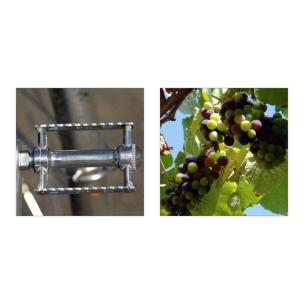
\includegraphics[interpolate=true,width=4.222222in,height=4.222222in]{figure1-img0.png}}%
\end{pgfscope}%
\begin{pgfscope}%
\definecolor{textcolor}{rgb}{0.000000,0.501961,0.000000}%
\pgfsetstrokecolor{textcolor}%
\pgfsetfillcolor{textcolor}%
\pgftext[x=1.630714in,y=4.342430in,,base]{\color{textcolor}\sffamily\fontsize{30.000000}{36.000000}\bfseries\selectfont 100}%
\end{pgfscope}%
\begin{pgfscope}%
\definecolor{textcolor}{rgb}{0.000000,0.000000,0.000000}%
\pgfsetstrokecolor{textcolor}%
\pgfsetfillcolor{textcolor}%
\pgftext[x=3.625851in,y=4.342430in,,base]{\color{textcolor}\sffamily\fontsize{30.000000}{36.000000}\bfseries\selectfont 2}%
\end{pgfscope}%
\begin{pgfscope}%
\definecolor{textcolor}{rgb}{0.000000,0.000000,0.000000}%
\pgfsetstrokecolor{textcolor}%
\pgfsetfillcolor{textcolor}%
\pgftext[x=0.100000in,y=6.072658in,left,base]{\color{textcolor}\sffamily\fontsize{35.000000}{42.000000}\bfseries\selectfont A}%
\end{pgfscope}%
\begin{pgfscope}%
\pgfsetbuttcap%
\pgfsetmiterjoin%
\definecolor{currentfill}{rgb}{1.000000,1.000000,1.000000}%
\pgfsetfillcolor{currentfill}%
\pgfsetlinewidth{0.000000pt}%
\definecolor{currentstroke}{rgb}{0.000000,0.000000,0.000000}%
\pgfsetstrokecolor{currentstroke}%
\pgfsetstrokeopacity{0.000000}%
\pgfsetdash{}{0pt}%
\pgfpathmoveto{\pgfqpoint{5.575543in}{0.764913in}}%
\pgfpathlineto{\pgfqpoint{9.787500in}{0.764913in}}%
\pgfpathlineto{\pgfqpoint{9.787500in}{5.483663in}}%
\pgfpathlineto{\pgfqpoint{5.575543in}{5.483663in}}%
\pgfpathlineto{\pgfqpoint{5.575543in}{0.764913in}}%
\pgfpathclose%
\pgfusepath{fill}%
\end{pgfscope}%
\begin{pgfscope}%
\pgfpathrectangle{\pgfqpoint{5.575543in}{0.764913in}}{\pgfqpoint{4.211957in}{4.718750in}}%
\pgfusepath{clip}%
\pgfsetbuttcap%
\pgfsetroundjoin%
\definecolor{currentfill}{rgb}{0.000000,0.000000,0.000000}%
\pgfsetfillcolor{currentfill}%
\pgfsetfillopacity{0.200000}%
\pgfsetlinewidth{1.003750pt}%
\definecolor{currentstroke}{rgb}{0.000000,0.000000,0.000000}%
\pgfsetstrokecolor{currentstroke}%
\pgfsetstrokeopacity{0.200000}%
\pgfsetdash{}{0pt}%
\pgfsys@defobject{currentmarker}{\pgfqpoint{5.602295in}{1.057000in}}{\pgfqpoint{9.588205in}{2.814391in}}{%
\pgfpathmoveto{\pgfqpoint{5.602295in}{2.814391in}}%
\pgfpathlineto{\pgfqpoint{5.602295in}{1.571145in}}%
\pgfpathlineto{\pgfqpoint{5.629046in}{1.807436in}}%
\pgfpathlineto{\pgfqpoint{5.655797in}{1.704790in}}%
\pgfpathlineto{\pgfqpoint{5.682548in}{1.641220in}}%
\pgfpathlineto{\pgfqpoint{5.709299in}{1.656006in}}%
\pgfpathlineto{\pgfqpoint{5.736050in}{1.567368in}}%
\pgfpathlineto{\pgfqpoint{5.762801in}{1.524279in}}%
\pgfpathlineto{\pgfqpoint{5.789552in}{1.455704in}}%
\pgfpathlineto{\pgfqpoint{5.816303in}{1.457646in}}%
\pgfpathlineto{\pgfqpoint{5.843054in}{1.445922in}}%
\pgfpathlineto{\pgfqpoint{5.869805in}{1.431602in}}%
\pgfpathlineto{\pgfqpoint{5.896556in}{1.444782in}}%
\pgfpathlineto{\pgfqpoint{5.923307in}{1.396025in}}%
\pgfpathlineto{\pgfqpoint{5.950059in}{1.435462in}}%
\pgfpathlineto{\pgfqpoint{5.976810in}{1.404176in}}%
\pgfpathlineto{\pgfqpoint{6.003561in}{1.387166in}}%
\pgfpathlineto{\pgfqpoint{6.030312in}{1.360669in}}%
\pgfpathlineto{\pgfqpoint{6.057063in}{1.350384in}}%
\pgfpathlineto{\pgfqpoint{6.083814in}{1.365284in}}%
\pgfpathlineto{\pgfqpoint{6.110565in}{1.345534in}}%
\pgfpathlineto{\pgfqpoint{6.137316in}{1.345758in}}%
\pgfpathlineto{\pgfqpoint{6.164067in}{1.357509in}}%
\pgfpathlineto{\pgfqpoint{6.190818in}{1.337111in}}%
\pgfpathlineto{\pgfqpoint{6.217569in}{1.344747in}}%
\pgfpathlineto{\pgfqpoint{6.244320in}{1.322974in}}%
\pgfpathlineto{\pgfqpoint{6.271071in}{1.328037in}}%
\pgfpathlineto{\pgfqpoint{6.297822in}{1.310640in}}%
\pgfpathlineto{\pgfqpoint{6.324574in}{1.294195in}}%
\pgfpathlineto{\pgfqpoint{6.351325in}{1.281704in}}%
\pgfpathlineto{\pgfqpoint{6.378076in}{1.284718in}}%
\pgfpathlineto{\pgfqpoint{6.404827in}{1.270208in}}%
\pgfpathlineto{\pgfqpoint{6.431578in}{1.281036in}}%
\pgfpathlineto{\pgfqpoint{6.458329in}{1.267857in}}%
\pgfpathlineto{\pgfqpoint{6.485080in}{1.260527in}}%
\pgfpathlineto{\pgfqpoint{6.511831in}{1.261197in}}%
\pgfpathlineto{\pgfqpoint{6.538582in}{1.262500in}}%
\pgfpathlineto{\pgfqpoint{6.565333in}{1.260745in}}%
\pgfpathlineto{\pgfqpoint{6.592084in}{1.253237in}}%
\pgfpathlineto{\pgfqpoint{6.618835in}{1.249985in}}%
\pgfpathlineto{\pgfqpoint{6.645586in}{1.240439in}}%
\pgfpathlineto{\pgfqpoint{6.672337in}{1.235037in}}%
\pgfpathlineto{\pgfqpoint{6.699089in}{1.227459in}}%
\pgfpathlineto{\pgfqpoint{6.725840in}{1.226447in}}%
\pgfpathlineto{\pgfqpoint{6.752591in}{1.217462in}}%
\pgfpathlineto{\pgfqpoint{6.779342in}{1.211106in}}%
\pgfpathlineto{\pgfqpoint{6.806093in}{1.212586in}}%
\pgfpathlineto{\pgfqpoint{6.832844in}{1.204077in}}%
\pgfpathlineto{\pgfqpoint{6.859595in}{1.203545in}}%
\pgfpathlineto{\pgfqpoint{6.886346in}{1.198751in}}%
\pgfpathlineto{\pgfqpoint{6.913097in}{1.195312in}}%
\pgfpathlineto{\pgfqpoint{6.939848in}{1.195622in}}%
\pgfpathlineto{\pgfqpoint{6.966599in}{1.190955in}}%
\pgfpathlineto{\pgfqpoint{6.993350in}{1.190117in}}%
\pgfpathlineto{\pgfqpoint{7.020101in}{1.178925in}}%
\pgfpathlineto{\pgfqpoint{7.046853in}{1.175897in}}%
\pgfpathlineto{\pgfqpoint{7.073604in}{1.168734in}}%
\pgfpathlineto{\pgfqpoint{7.100355in}{1.169616in}}%
\pgfpathlineto{\pgfqpoint{7.127106in}{1.163492in}}%
\pgfpathlineto{\pgfqpoint{7.153857in}{1.154902in}}%
\pgfpathlineto{\pgfqpoint{7.180608in}{1.156994in}}%
\pgfpathlineto{\pgfqpoint{7.207359in}{1.153157in}}%
\pgfpathlineto{\pgfqpoint{7.234110in}{1.143720in}}%
\pgfpathlineto{\pgfqpoint{7.260861in}{1.147795in}}%
\pgfpathlineto{\pgfqpoint{7.287612in}{1.152113in}}%
\pgfpathlineto{\pgfqpoint{7.314363in}{1.143784in}}%
\pgfpathlineto{\pgfqpoint{7.341114in}{1.141492in}}%
\pgfpathlineto{\pgfqpoint{7.367865in}{1.141413in}}%
\pgfpathlineto{\pgfqpoint{7.394616in}{1.142144in}}%
\pgfpathlineto{\pgfqpoint{7.421368in}{1.142367in}}%
\pgfpathlineto{\pgfqpoint{7.448119in}{1.144088in}}%
\pgfpathlineto{\pgfqpoint{7.474870in}{1.133135in}}%
\pgfpathlineto{\pgfqpoint{7.501621in}{1.138295in}}%
\pgfpathlineto{\pgfqpoint{7.528372in}{1.136004in}}%
\pgfpathlineto{\pgfqpoint{7.555123in}{1.136700in}}%
\pgfpathlineto{\pgfqpoint{7.581874in}{1.135843in}}%
\pgfpathlineto{\pgfqpoint{7.608625in}{1.135374in}}%
\pgfpathlineto{\pgfqpoint{7.635376in}{1.128564in}}%
\pgfpathlineto{\pgfqpoint{7.662127in}{1.126053in}}%
\pgfpathlineto{\pgfqpoint{7.688878in}{1.126708in}}%
\pgfpathlineto{\pgfqpoint{7.715629in}{1.123503in}}%
\pgfpathlineto{\pgfqpoint{7.742380in}{1.125294in}}%
\pgfpathlineto{\pgfqpoint{7.769132in}{1.123121in}}%
\pgfpathlineto{\pgfqpoint{7.795883in}{1.121514in}}%
\pgfpathlineto{\pgfqpoint{7.822634in}{1.122437in}}%
\pgfpathlineto{\pgfqpoint{7.849385in}{1.118388in}}%
\pgfpathlineto{\pgfqpoint{7.876136in}{1.117610in}}%
\pgfpathlineto{\pgfqpoint{7.902887in}{1.108327in}}%
\pgfpathlineto{\pgfqpoint{7.929638in}{1.115435in}}%
\pgfpathlineto{\pgfqpoint{7.956389in}{1.116231in}}%
\pgfpathlineto{\pgfqpoint{7.983140in}{1.116542in}}%
\pgfpathlineto{\pgfqpoint{8.009891in}{1.113259in}}%
\pgfpathlineto{\pgfqpoint{8.036642in}{1.107465in}}%
\pgfpathlineto{\pgfqpoint{8.063393in}{1.115654in}}%
\pgfpathlineto{\pgfqpoint{8.090144in}{1.105690in}}%
\pgfpathlineto{\pgfqpoint{8.116895in}{1.110482in}}%
\pgfpathlineto{\pgfqpoint{8.143647in}{1.104557in}}%
\pgfpathlineto{\pgfqpoint{8.170398in}{1.107675in}}%
\pgfpathlineto{\pgfqpoint{8.197149in}{1.105437in}}%
\pgfpathlineto{\pgfqpoint{8.223900in}{1.098585in}}%
\pgfpathlineto{\pgfqpoint{8.250651in}{1.103602in}}%
\pgfpathlineto{\pgfqpoint{8.277402in}{1.101135in}}%
\pgfpathlineto{\pgfqpoint{8.304153in}{1.097572in}}%
\pgfpathlineto{\pgfqpoint{8.330904in}{1.103818in}}%
\pgfpathlineto{\pgfqpoint{8.357655in}{1.096974in}}%
\pgfpathlineto{\pgfqpoint{8.384406in}{1.089923in}}%
\pgfpathlineto{\pgfqpoint{8.411157in}{1.092333in}}%
\pgfpathlineto{\pgfqpoint{8.437908in}{1.090519in}}%
\pgfpathlineto{\pgfqpoint{8.464659in}{1.084965in}}%
\pgfpathlineto{\pgfqpoint{8.491410in}{1.091097in}}%
\pgfpathlineto{\pgfqpoint{8.518162in}{1.090967in}}%
\pgfpathlineto{\pgfqpoint{8.544913in}{1.081466in}}%
\pgfpathlineto{\pgfqpoint{8.571664in}{1.087853in}}%
\pgfpathlineto{\pgfqpoint{8.598415in}{1.089211in}}%
\pgfpathlineto{\pgfqpoint{8.625166in}{1.085699in}}%
\pgfpathlineto{\pgfqpoint{8.651917in}{1.078772in}}%
\pgfpathlineto{\pgfqpoint{8.678668in}{1.086099in}}%
\pgfpathlineto{\pgfqpoint{8.705419in}{1.080200in}}%
\pgfpathlineto{\pgfqpoint{8.732170in}{1.079880in}}%
\pgfpathlineto{\pgfqpoint{8.758921in}{1.078563in}}%
\pgfpathlineto{\pgfqpoint{8.785672in}{1.072648in}}%
\pgfpathlineto{\pgfqpoint{8.812423in}{1.079245in}}%
\pgfpathlineto{\pgfqpoint{8.839174in}{1.073496in}}%
\pgfpathlineto{\pgfqpoint{8.865926in}{1.079627in}}%
\pgfpathlineto{\pgfqpoint{8.892677in}{1.074758in}}%
\pgfpathlineto{\pgfqpoint{8.919428in}{1.075716in}}%
\pgfpathlineto{\pgfqpoint{8.946179in}{1.075316in}}%
\pgfpathlineto{\pgfqpoint{8.972930in}{1.076225in}}%
\pgfpathlineto{\pgfqpoint{8.999681in}{1.079440in}}%
\pgfpathlineto{\pgfqpoint{9.026432in}{1.067034in}}%
\pgfpathlineto{\pgfqpoint{9.053183in}{1.067283in}}%
\pgfpathlineto{\pgfqpoint{9.079934in}{1.065796in}}%
\pgfpathlineto{\pgfqpoint{9.106685in}{1.062896in}}%
\pgfpathlineto{\pgfqpoint{9.133436in}{1.063192in}}%
\pgfpathlineto{\pgfqpoint{9.160187in}{1.071464in}}%
\pgfpathlineto{\pgfqpoint{9.186938in}{1.066047in}}%
\pgfpathlineto{\pgfqpoint{9.213689in}{1.071205in}}%
\pgfpathlineto{\pgfqpoint{9.240441in}{1.066358in}}%
\pgfpathlineto{\pgfqpoint{9.267192in}{1.061475in}}%
\pgfpathlineto{\pgfqpoint{9.293943in}{1.061670in}}%
\pgfpathlineto{\pgfqpoint{9.320694in}{1.060105in}}%
\pgfpathlineto{\pgfqpoint{9.347445in}{1.063549in}}%
\pgfpathlineto{\pgfqpoint{9.374196in}{1.064701in}}%
\pgfpathlineto{\pgfqpoint{9.400947in}{1.062393in}}%
\pgfpathlineto{\pgfqpoint{9.427698in}{1.065109in}}%
\pgfpathlineto{\pgfqpoint{9.454449in}{1.063792in}}%
\pgfpathlineto{\pgfqpoint{9.481200in}{1.062732in}}%
\pgfpathlineto{\pgfqpoint{9.507951in}{1.060577in}}%
\pgfpathlineto{\pgfqpoint{9.534702in}{1.062668in}}%
\pgfpathlineto{\pgfqpoint{9.561453in}{1.061269in}}%
\pgfpathlineto{\pgfqpoint{9.588205in}{1.057000in}}%
\pgfpathlineto{\pgfqpoint{9.588205in}{1.224453in}}%
\pgfpathlineto{\pgfqpoint{9.588205in}{1.224453in}}%
\pgfpathlineto{\pgfqpoint{9.561453in}{1.222996in}}%
\pgfpathlineto{\pgfqpoint{9.534702in}{1.222359in}}%
\pgfpathlineto{\pgfqpoint{9.507951in}{1.222096in}}%
\pgfpathlineto{\pgfqpoint{9.481200in}{1.228078in}}%
\pgfpathlineto{\pgfqpoint{9.454449in}{1.223129in}}%
\pgfpathlineto{\pgfqpoint{9.427698in}{1.224491in}}%
\pgfpathlineto{\pgfqpoint{9.400947in}{1.226366in}}%
\pgfpathlineto{\pgfqpoint{9.374196in}{1.225894in}}%
\pgfpathlineto{\pgfqpoint{9.347445in}{1.228062in}}%
\pgfpathlineto{\pgfqpoint{9.320694in}{1.218784in}}%
\pgfpathlineto{\pgfqpoint{9.293943in}{1.221912in}}%
\pgfpathlineto{\pgfqpoint{9.267192in}{1.224621in}}%
\pgfpathlineto{\pgfqpoint{9.240441in}{1.223973in}}%
\pgfpathlineto{\pgfqpoint{9.213689in}{1.224672in}}%
\pgfpathlineto{\pgfqpoint{9.186938in}{1.236824in}}%
\pgfpathlineto{\pgfqpoint{9.160187in}{1.234607in}}%
\pgfpathlineto{\pgfqpoint{9.133436in}{1.228281in}}%
\pgfpathlineto{\pgfqpoint{9.106685in}{1.233408in}}%
\pgfpathlineto{\pgfqpoint{9.079934in}{1.236865in}}%
\pgfpathlineto{\pgfqpoint{9.053183in}{1.240026in}}%
\pgfpathlineto{\pgfqpoint{9.026432in}{1.235208in}}%
\pgfpathlineto{\pgfqpoint{8.999681in}{1.238389in}}%
\pgfpathlineto{\pgfqpoint{8.972930in}{1.245151in}}%
\pgfpathlineto{\pgfqpoint{8.946179in}{1.241211in}}%
\pgfpathlineto{\pgfqpoint{8.919428in}{1.240343in}}%
\pgfpathlineto{\pgfqpoint{8.892677in}{1.244949in}}%
\pgfpathlineto{\pgfqpoint{8.865926in}{1.243900in}}%
\pgfpathlineto{\pgfqpoint{8.839174in}{1.244481in}}%
\pgfpathlineto{\pgfqpoint{8.812423in}{1.254058in}}%
\pgfpathlineto{\pgfqpoint{8.785672in}{1.242373in}}%
\pgfpathlineto{\pgfqpoint{8.758921in}{1.255317in}}%
\pgfpathlineto{\pgfqpoint{8.732170in}{1.248950in}}%
\pgfpathlineto{\pgfqpoint{8.705419in}{1.250118in}}%
\pgfpathlineto{\pgfqpoint{8.678668in}{1.261481in}}%
\pgfpathlineto{\pgfqpoint{8.651917in}{1.250954in}}%
\pgfpathlineto{\pgfqpoint{8.625166in}{1.257353in}}%
\pgfpathlineto{\pgfqpoint{8.598415in}{1.265260in}}%
\pgfpathlineto{\pgfqpoint{8.571664in}{1.260597in}}%
\pgfpathlineto{\pgfqpoint{8.544913in}{1.262560in}}%
\pgfpathlineto{\pgfqpoint{8.518162in}{1.277359in}}%
\pgfpathlineto{\pgfqpoint{8.491410in}{1.262640in}}%
\pgfpathlineto{\pgfqpoint{8.464659in}{1.262996in}}%
\pgfpathlineto{\pgfqpoint{8.437908in}{1.265974in}}%
\pgfpathlineto{\pgfqpoint{8.411157in}{1.267231in}}%
\pgfpathlineto{\pgfqpoint{8.384406in}{1.270288in}}%
\pgfpathlineto{\pgfqpoint{8.357655in}{1.274698in}}%
\pgfpathlineto{\pgfqpoint{8.330904in}{1.274556in}}%
\pgfpathlineto{\pgfqpoint{8.304153in}{1.282223in}}%
\pgfpathlineto{\pgfqpoint{8.277402in}{1.291704in}}%
\pgfpathlineto{\pgfqpoint{8.250651in}{1.286020in}}%
\pgfpathlineto{\pgfqpoint{8.223900in}{1.290287in}}%
\pgfpathlineto{\pgfqpoint{8.197149in}{1.294356in}}%
\pgfpathlineto{\pgfqpoint{8.170398in}{1.292529in}}%
\pgfpathlineto{\pgfqpoint{8.143647in}{1.294506in}}%
\pgfpathlineto{\pgfqpoint{8.116895in}{1.300207in}}%
\pgfpathlineto{\pgfqpoint{8.090144in}{1.301776in}}%
\pgfpathlineto{\pgfqpoint{8.063393in}{1.298295in}}%
\pgfpathlineto{\pgfqpoint{8.036642in}{1.297916in}}%
\pgfpathlineto{\pgfqpoint{8.009891in}{1.304523in}}%
\pgfpathlineto{\pgfqpoint{7.983140in}{1.300506in}}%
\pgfpathlineto{\pgfqpoint{7.956389in}{1.300774in}}%
\pgfpathlineto{\pgfqpoint{7.929638in}{1.294790in}}%
\pgfpathlineto{\pgfqpoint{7.902887in}{1.292783in}}%
\pgfpathlineto{\pgfqpoint{7.876136in}{1.294491in}}%
\pgfpathlineto{\pgfqpoint{7.849385in}{1.295236in}}%
\pgfpathlineto{\pgfqpoint{7.822634in}{1.293353in}}%
\pgfpathlineto{\pgfqpoint{7.795883in}{1.291751in}}%
\pgfpathlineto{\pgfqpoint{7.769132in}{1.303296in}}%
\pgfpathlineto{\pgfqpoint{7.742380in}{1.298483in}}%
\pgfpathlineto{\pgfqpoint{7.715629in}{1.304001in}}%
\pgfpathlineto{\pgfqpoint{7.688878in}{1.302333in}}%
\pgfpathlineto{\pgfqpoint{7.662127in}{1.305373in}}%
\pgfpathlineto{\pgfqpoint{7.635376in}{1.304310in}}%
\pgfpathlineto{\pgfqpoint{7.608625in}{1.306740in}}%
\pgfpathlineto{\pgfqpoint{7.581874in}{1.323188in}}%
\pgfpathlineto{\pgfqpoint{7.555123in}{1.312981in}}%
\pgfpathlineto{\pgfqpoint{7.528372in}{1.326136in}}%
\pgfpathlineto{\pgfqpoint{7.501621in}{1.321129in}}%
\pgfpathlineto{\pgfqpoint{7.474870in}{1.322680in}}%
\pgfpathlineto{\pgfqpoint{7.448119in}{1.328351in}}%
\pgfpathlineto{\pgfqpoint{7.421368in}{1.329958in}}%
\pgfpathlineto{\pgfqpoint{7.394616in}{1.323387in}}%
\pgfpathlineto{\pgfqpoint{7.367865in}{1.331161in}}%
\pgfpathlineto{\pgfqpoint{7.341114in}{1.331928in}}%
\pgfpathlineto{\pgfqpoint{7.314363in}{1.331900in}}%
\pgfpathlineto{\pgfqpoint{7.287612in}{1.335537in}}%
\pgfpathlineto{\pgfqpoint{7.260861in}{1.325354in}}%
\pgfpathlineto{\pgfqpoint{7.234110in}{1.347120in}}%
\pgfpathlineto{\pgfqpoint{7.207359in}{1.341507in}}%
\pgfpathlineto{\pgfqpoint{7.180608in}{1.346749in}}%
\pgfpathlineto{\pgfqpoint{7.153857in}{1.354913in}}%
\pgfpathlineto{\pgfqpoint{7.127106in}{1.357387in}}%
\pgfpathlineto{\pgfqpoint{7.100355in}{1.367013in}}%
\pgfpathlineto{\pgfqpoint{7.073604in}{1.371457in}}%
\pgfpathlineto{\pgfqpoint{7.046853in}{1.369569in}}%
\pgfpathlineto{\pgfqpoint{7.020101in}{1.362750in}}%
\pgfpathlineto{\pgfqpoint{6.993350in}{1.376762in}}%
\pgfpathlineto{\pgfqpoint{6.966599in}{1.377985in}}%
\pgfpathlineto{\pgfqpoint{6.939848in}{1.390833in}}%
\pgfpathlineto{\pgfqpoint{6.913097in}{1.393366in}}%
\pgfpathlineto{\pgfqpoint{6.886346in}{1.399222in}}%
\pgfpathlineto{\pgfqpoint{6.859595in}{1.405597in}}%
\pgfpathlineto{\pgfqpoint{6.832844in}{1.404797in}}%
\pgfpathlineto{\pgfqpoint{6.806093in}{1.403348in}}%
\pgfpathlineto{\pgfqpoint{6.779342in}{1.409842in}}%
\pgfpathlineto{\pgfqpoint{6.752591in}{1.427130in}}%
\pgfpathlineto{\pgfqpoint{6.725840in}{1.432066in}}%
\pgfpathlineto{\pgfqpoint{6.699089in}{1.449916in}}%
\pgfpathlineto{\pgfqpoint{6.672337in}{1.455551in}}%
\pgfpathlineto{\pgfqpoint{6.645586in}{1.455465in}}%
\pgfpathlineto{\pgfqpoint{6.618835in}{1.471985in}}%
\pgfpathlineto{\pgfqpoint{6.592084in}{1.458688in}}%
\pgfpathlineto{\pgfqpoint{6.565333in}{1.480235in}}%
\pgfpathlineto{\pgfqpoint{6.538582in}{1.479681in}}%
\pgfpathlineto{\pgfqpoint{6.511831in}{1.493338in}}%
\pgfpathlineto{\pgfqpoint{6.485080in}{1.501652in}}%
\pgfpathlineto{\pgfqpoint{6.458329in}{1.510979in}}%
\pgfpathlineto{\pgfqpoint{6.431578in}{1.532390in}}%
\pgfpathlineto{\pgfqpoint{6.404827in}{1.532219in}}%
\pgfpathlineto{\pgfqpoint{6.378076in}{1.525961in}}%
\pgfpathlineto{\pgfqpoint{6.351325in}{1.534790in}}%
\pgfpathlineto{\pgfqpoint{6.324574in}{1.563205in}}%
\pgfpathlineto{\pgfqpoint{6.297822in}{1.572893in}}%
\pgfpathlineto{\pgfqpoint{6.271071in}{1.602959in}}%
\pgfpathlineto{\pgfqpoint{6.244320in}{1.605947in}}%
\pgfpathlineto{\pgfqpoint{6.217569in}{1.635306in}}%
\pgfpathlineto{\pgfqpoint{6.190818in}{1.641395in}}%
\pgfpathlineto{\pgfqpoint{6.164067in}{1.669098in}}%
\pgfpathlineto{\pgfqpoint{6.137316in}{1.686046in}}%
\pgfpathlineto{\pgfqpoint{6.110565in}{1.684270in}}%
\pgfpathlineto{\pgfqpoint{6.083814in}{1.680374in}}%
\pgfpathlineto{\pgfqpoint{6.057063in}{1.691579in}}%
\pgfpathlineto{\pgfqpoint{6.030312in}{1.719902in}}%
\pgfpathlineto{\pgfqpoint{6.003561in}{1.771752in}}%
\pgfpathlineto{\pgfqpoint{5.976810in}{1.761483in}}%
\pgfpathlineto{\pgfqpoint{5.950059in}{1.791042in}}%
\pgfpathlineto{\pgfqpoint{5.923307in}{1.764587in}}%
\pgfpathlineto{\pgfqpoint{5.896556in}{1.820388in}}%
\pgfpathlineto{\pgfqpoint{5.869805in}{1.840736in}}%
\pgfpathlineto{\pgfqpoint{5.843054in}{1.819878in}}%
\pgfpathlineto{\pgfqpoint{5.816303in}{1.831279in}}%
\pgfpathlineto{\pgfqpoint{5.789552in}{1.829160in}}%
\pgfpathlineto{\pgfqpoint{5.762801in}{1.905181in}}%
\pgfpathlineto{\pgfqpoint{5.736050in}{2.010909in}}%
\pgfpathlineto{\pgfqpoint{5.709299in}{2.071025in}}%
\pgfpathlineto{\pgfqpoint{5.682548in}{2.056647in}}%
\pgfpathlineto{\pgfqpoint{5.655797in}{2.232241in}}%
\pgfpathlineto{\pgfqpoint{5.629046in}{2.520416in}}%
\pgfpathlineto{\pgfqpoint{5.602295in}{2.814391in}}%
\pgfpathlineto{\pgfqpoint{5.602295in}{2.814391in}}%
\pgfpathclose%
\pgfusepath{stroke,fill}%
}%
\begin{pgfscope}%
\pgfsys@transformshift{0.000000in}{0.000000in}%
\pgfsys@useobject{currentmarker}{}%
\end{pgfscope}%
\end{pgfscope}%
\begin{pgfscope}%
\pgfsetbuttcap%
\pgfsetroundjoin%
\definecolor{currentfill}{rgb}{0.000000,0.000000,0.000000}%
\pgfsetfillcolor{currentfill}%
\pgfsetlinewidth{0.803000pt}%
\definecolor{currentstroke}{rgb}{0.000000,0.000000,0.000000}%
\pgfsetstrokecolor{currentstroke}%
\pgfsetdash{}{0pt}%
\pgfsys@defobject{currentmarker}{\pgfqpoint{0.000000in}{-0.048611in}}{\pgfqpoint{0.000000in}{0.000000in}}{%
\pgfpathmoveto{\pgfqpoint{0.000000in}{0.000000in}}%
\pgfpathlineto{\pgfqpoint{0.000000in}{-0.048611in}}%
\pgfusepath{stroke,fill}%
}%
\begin{pgfscope}%
\pgfsys@transformshift{5.575543in}{0.764913in}%
\pgfsys@useobject{currentmarker}{}%
\end{pgfscope}%
\end{pgfscope}%
\begin{pgfscope}%
\definecolor{textcolor}{rgb}{0.000000,0.000000,0.000000}%
\pgfsetstrokecolor{textcolor}%
\pgfsetfillcolor{textcolor}%
\pgftext[x=5.575543in,y=0.667691in,,top]{\color{textcolor}\sffamily\fontsize{20.000000}{24.000000}\selectfont 0}%
\end{pgfscope}%
\begin{pgfscope}%
\pgfsetbuttcap%
\pgfsetroundjoin%
\definecolor{currentfill}{rgb}{0.000000,0.000000,0.000000}%
\pgfsetfillcolor{currentfill}%
\pgfsetlinewidth{0.803000pt}%
\definecolor{currentstroke}{rgb}{0.000000,0.000000,0.000000}%
\pgfsetstrokecolor{currentstroke}%
\pgfsetdash{}{0pt}%
\pgfsys@defobject{currentmarker}{\pgfqpoint{0.000000in}{-0.048611in}}{\pgfqpoint{0.000000in}{0.000000in}}{%
\pgfpathmoveto{\pgfqpoint{0.000000in}{0.000000in}}%
\pgfpathlineto{\pgfqpoint{0.000000in}{-0.048611in}}%
\pgfusepath{stroke,fill}%
}%
\begin{pgfscope}%
\pgfsys@transformshift{6.913097in}{0.764913in}%
\pgfsys@useobject{currentmarker}{}%
\end{pgfscope}%
\end{pgfscope}%
\begin{pgfscope}%
\definecolor{textcolor}{rgb}{0.000000,0.000000,0.000000}%
\pgfsetstrokecolor{textcolor}%
\pgfsetfillcolor{textcolor}%
\pgftext[x=6.913097in,y=0.667691in,,top]{\color{textcolor}\sffamily\fontsize{20.000000}{24.000000}\selectfont 50}%
\end{pgfscope}%
\begin{pgfscope}%
\pgfsetbuttcap%
\pgfsetroundjoin%
\definecolor{currentfill}{rgb}{0.000000,0.000000,0.000000}%
\pgfsetfillcolor{currentfill}%
\pgfsetlinewidth{0.803000pt}%
\definecolor{currentstroke}{rgb}{0.000000,0.000000,0.000000}%
\pgfsetstrokecolor{currentstroke}%
\pgfsetdash{}{0pt}%
\pgfsys@defobject{currentmarker}{\pgfqpoint{0.000000in}{-0.048611in}}{\pgfqpoint{0.000000in}{0.000000in}}{%
\pgfpathmoveto{\pgfqpoint{0.000000in}{0.000000in}}%
\pgfpathlineto{\pgfqpoint{0.000000in}{-0.048611in}}%
\pgfusepath{stroke,fill}%
}%
\begin{pgfscope}%
\pgfsys@transformshift{8.250651in}{0.764913in}%
\pgfsys@useobject{currentmarker}{}%
\end{pgfscope}%
\end{pgfscope}%
\begin{pgfscope}%
\definecolor{textcolor}{rgb}{0.000000,0.000000,0.000000}%
\pgfsetstrokecolor{textcolor}%
\pgfsetfillcolor{textcolor}%
\pgftext[x=8.250651in,y=0.667691in,,top]{\color{textcolor}\sffamily\fontsize{20.000000}{24.000000}\selectfont 100}%
\end{pgfscope}%
\begin{pgfscope}%
\pgfsetbuttcap%
\pgfsetroundjoin%
\definecolor{currentfill}{rgb}{0.000000,0.000000,0.000000}%
\pgfsetfillcolor{currentfill}%
\pgfsetlinewidth{0.803000pt}%
\definecolor{currentstroke}{rgb}{0.000000,0.000000,0.000000}%
\pgfsetstrokecolor{currentstroke}%
\pgfsetdash{}{0pt}%
\pgfsys@defobject{currentmarker}{\pgfqpoint{0.000000in}{-0.048611in}}{\pgfqpoint{0.000000in}{0.000000in}}{%
\pgfpathmoveto{\pgfqpoint{0.000000in}{0.000000in}}%
\pgfpathlineto{\pgfqpoint{0.000000in}{-0.048611in}}%
\pgfusepath{stroke,fill}%
}%
\begin{pgfscope}%
\pgfsys@transformshift{9.588205in}{0.764913in}%
\pgfsys@useobject{currentmarker}{}%
\end{pgfscope}%
\end{pgfscope}%
\begin{pgfscope}%
\definecolor{textcolor}{rgb}{0.000000,0.000000,0.000000}%
\pgfsetstrokecolor{textcolor}%
\pgfsetfillcolor{textcolor}%
\pgftext[x=9.588205in,y=0.667691in,,top]{\color{textcolor}\sffamily\fontsize{20.000000}{24.000000}\selectfont 150}%
\end{pgfscope}%
\begin{pgfscope}%
\definecolor{textcolor}{rgb}{0.000000,0.000000,0.000000}%
\pgfsetstrokecolor{textcolor}%
\pgfsetfillcolor{textcolor}%
\pgftext[x=7.681522in,y=0.356068in,,top]{\color{textcolor}\sffamily\fontsize{20.000000}{24.000000}\selectfont Trial}%
\end{pgfscope}%
\begin{pgfscope}%
\pgfsetbuttcap%
\pgfsetroundjoin%
\definecolor{currentfill}{rgb}{0.000000,0.000000,0.000000}%
\pgfsetfillcolor{currentfill}%
\pgfsetlinewidth{0.803000pt}%
\definecolor{currentstroke}{rgb}{0.000000,0.000000,0.000000}%
\pgfsetstrokecolor{currentstroke}%
\pgfsetdash{}{0pt}%
\pgfsys@defobject{currentmarker}{\pgfqpoint{-0.048611in}{0.000000in}}{\pgfqpoint{-0.000000in}{0.000000in}}{%
\pgfpathmoveto{\pgfqpoint{-0.000000in}{0.000000in}}%
\pgfpathlineto{\pgfqpoint{-0.048611in}{0.000000in}}%
\pgfusepath{stroke,fill}%
}%
\begin{pgfscope}%
\pgfsys@transformshift{5.575543in}{0.764913in}%
\pgfsys@useobject{currentmarker}{}%
\end{pgfscope}%
\end{pgfscope}%
\begin{pgfscope}%
\definecolor{textcolor}{rgb}{0.000000,0.000000,0.000000}%
\pgfsetstrokecolor{textcolor}%
\pgfsetfillcolor{textcolor}%
\pgftext[x=5.342880in, y=0.664894in, left, base]{\color{textcolor}\sffamily\fontsize{20.000000}{24.000000}\selectfont 0}%
\end{pgfscope}%
\begin{pgfscope}%
\pgfsetbuttcap%
\pgfsetroundjoin%
\definecolor{currentfill}{rgb}{0.000000,0.000000,0.000000}%
\pgfsetfillcolor{currentfill}%
\pgfsetlinewidth{0.803000pt}%
\definecolor{currentstroke}{rgb}{0.000000,0.000000,0.000000}%
\pgfsetstrokecolor{currentstroke}%
\pgfsetdash{}{0pt}%
\pgfsys@defobject{currentmarker}{\pgfqpoint{-0.048611in}{0.000000in}}{\pgfqpoint{-0.000000in}{0.000000in}}{%
\pgfpathmoveto{\pgfqpoint{-0.000000in}{0.000000in}}%
\pgfpathlineto{\pgfqpoint{-0.048611in}{0.000000in}}%
\pgfusepath{stroke,fill}%
}%
\begin{pgfscope}%
\pgfsys@transformshift{5.575543in}{1.406920in}%
\pgfsys@useobject{currentmarker}{}%
\end{pgfscope}%
\end{pgfscope}%
\begin{pgfscope}%
\definecolor{textcolor}{rgb}{0.000000,0.000000,0.000000}%
\pgfsetstrokecolor{textcolor}%
\pgfsetfillcolor{textcolor}%
\pgftext[x=5.207438in, y=1.306901in, left, base]{\color{textcolor}\sffamily\fontsize{20.000000}{24.000000}\selectfont 10}%
\end{pgfscope}%
\begin{pgfscope}%
\pgfsetbuttcap%
\pgfsetroundjoin%
\definecolor{currentfill}{rgb}{0.000000,0.000000,0.000000}%
\pgfsetfillcolor{currentfill}%
\pgfsetlinewidth{0.803000pt}%
\definecolor{currentstroke}{rgb}{0.000000,0.000000,0.000000}%
\pgfsetstrokecolor{currentstroke}%
\pgfsetdash{}{0pt}%
\pgfsys@defobject{currentmarker}{\pgfqpoint{-0.048611in}{0.000000in}}{\pgfqpoint{-0.000000in}{0.000000in}}{%
\pgfpathmoveto{\pgfqpoint{-0.000000in}{0.000000in}}%
\pgfpathlineto{\pgfqpoint{-0.048611in}{0.000000in}}%
\pgfusepath{stroke,fill}%
}%
\begin{pgfscope}%
\pgfsys@transformshift{5.575543in}{2.048927in}%
\pgfsys@useobject{currentmarker}{}%
\end{pgfscope}%
\end{pgfscope}%
\begin{pgfscope}%
\definecolor{textcolor}{rgb}{0.000000,0.000000,0.000000}%
\pgfsetstrokecolor{textcolor}%
\pgfsetfillcolor{textcolor}%
\pgftext[x=5.207438in, y=1.948907in, left, base]{\color{textcolor}\sffamily\fontsize{20.000000}{24.000000}\selectfont 20}%
\end{pgfscope}%
\begin{pgfscope}%
\pgfsetbuttcap%
\pgfsetroundjoin%
\definecolor{currentfill}{rgb}{0.000000,0.000000,0.000000}%
\pgfsetfillcolor{currentfill}%
\pgfsetlinewidth{0.803000pt}%
\definecolor{currentstroke}{rgb}{0.000000,0.000000,0.000000}%
\pgfsetstrokecolor{currentstroke}%
\pgfsetdash{}{0pt}%
\pgfsys@defobject{currentmarker}{\pgfqpoint{-0.048611in}{0.000000in}}{\pgfqpoint{-0.000000in}{0.000000in}}{%
\pgfpathmoveto{\pgfqpoint{-0.000000in}{0.000000in}}%
\pgfpathlineto{\pgfqpoint{-0.048611in}{0.000000in}}%
\pgfusepath{stroke,fill}%
}%
\begin{pgfscope}%
\pgfsys@transformshift{5.575543in}{2.690933in}%
\pgfsys@useobject{currentmarker}{}%
\end{pgfscope}%
\end{pgfscope}%
\begin{pgfscope}%
\definecolor{textcolor}{rgb}{0.000000,0.000000,0.000000}%
\pgfsetstrokecolor{textcolor}%
\pgfsetfillcolor{textcolor}%
\pgftext[x=5.207438in, y=2.590914in, left, base]{\color{textcolor}\sffamily\fontsize{20.000000}{24.000000}\selectfont 30}%
\end{pgfscope}%
\begin{pgfscope}%
\pgfsetbuttcap%
\pgfsetroundjoin%
\definecolor{currentfill}{rgb}{0.000000,0.000000,0.000000}%
\pgfsetfillcolor{currentfill}%
\pgfsetlinewidth{0.803000pt}%
\definecolor{currentstroke}{rgb}{0.000000,0.000000,0.000000}%
\pgfsetstrokecolor{currentstroke}%
\pgfsetdash{}{0pt}%
\pgfsys@defobject{currentmarker}{\pgfqpoint{-0.048611in}{0.000000in}}{\pgfqpoint{-0.000000in}{0.000000in}}{%
\pgfpathmoveto{\pgfqpoint{-0.000000in}{0.000000in}}%
\pgfpathlineto{\pgfqpoint{-0.048611in}{0.000000in}}%
\pgfusepath{stroke,fill}%
}%
\begin{pgfscope}%
\pgfsys@transformshift{5.575543in}{3.332940in}%
\pgfsys@useobject{currentmarker}{}%
\end{pgfscope}%
\end{pgfscope}%
\begin{pgfscope}%
\definecolor{textcolor}{rgb}{0.000000,0.000000,0.000000}%
\pgfsetstrokecolor{textcolor}%
\pgfsetfillcolor{textcolor}%
\pgftext[x=5.207438in, y=3.232921in, left, base]{\color{textcolor}\sffamily\fontsize{20.000000}{24.000000}\selectfont 40}%
\end{pgfscope}%
\begin{pgfscope}%
\pgfsetbuttcap%
\pgfsetroundjoin%
\definecolor{currentfill}{rgb}{0.000000,0.000000,0.000000}%
\pgfsetfillcolor{currentfill}%
\pgfsetlinewidth{0.803000pt}%
\definecolor{currentstroke}{rgb}{0.000000,0.000000,0.000000}%
\pgfsetstrokecolor{currentstroke}%
\pgfsetdash{}{0pt}%
\pgfsys@defobject{currentmarker}{\pgfqpoint{-0.048611in}{0.000000in}}{\pgfqpoint{-0.000000in}{0.000000in}}{%
\pgfpathmoveto{\pgfqpoint{-0.000000in}{0.000000in}}%
\pgfpathlineto{\pgfqpoint{-0.048611in}{0.000000in}}%
\pgfusepath{stroke,fill}%
}%
\begin{pgfscope}%
\pgfsys@transformshift{5.575543in}{3.974947in}%
\pgfsys@useobject{currentmarker}{}%
\end{pgfscope}%
\end{pgfscope}%
\begin{pgfscope}%
\definecolor{textcolor}{rgb}{0.000000,0.000000,0.000000}%
\pgfsetstrokecolor{textcolor}%
\pgfsetfillcolor{textcolor}%
\pgftext[x=5.207438in, y=3.874928in, left, base]{\color{textcolor}\sffamily\fontsize{20.000000}{24.000000}\selectfont 50}%
\end{pgfscope}%
\begin{pgfscope}%
\pgfsetbuttcap%
\pgfsetroundjoin%
\definecolor{currentfill}{rgb}{0.000000,0.000000,0.000000}%
\pgfsetfillcolor{currentfill}%
\pgfsetlinewidth{0.803000pt}%
\definecolor{currentstroke}{rgb}{0.000000,0.000000,0.000000}%
\pgfsetstrokecolor{currentstroke}%
\pgfsetdash{}{0pt}%
\pgfsys@defobject{currentmarker}{\pgfqpoint{-0.048611in}{0.000000in}}{\pgfqpoint{-0.000000in}{0.000000in}}{%
\pgfpathmoveto{\pgfqpoint{-0.000000in}{0.000000in}}%
\pgfpathlineto{\pgfqpoint{-0.048611in}{0.000000in}}%
\pgfusepath{stroke,fill}%
}%
\begin{pgfscope}%
\pgfsys@transformshift{5.575543in}{4.616954in}%
\pgfsys@useobject{currentmarker}{}%
\end{pgfscope}%
\end{pgfscope}%
\begin{pgfscope}%
\definecolor{textcolor}{rgb}{0.000000,0.000000,0.000000}%
\pgfsetstrokecolor{textcolor}%
\pgfsetfillcolor{textcolor}%
\pgftext[x=5.207438in, y=4.516935in, left, base]{\color{textcolor}\sffamily\fontsize{20.000000}{24.000000}\selectfont 60}%
\end{pgfscope}%
\begin{pgfscope}%
\pgfsetbuttcap%
\pgfsetroundjoin%
\definecolor{currentfill}{rgb}{0.000000,0.000000,0.000000}%
\pgfsetfillcolor{currentfill}%
\pgfsetlinewidth{0.803000pt}%
\definecolor{currentstroke}{rgb}{0.000000,0.000000,0.000000}%
\pgfsetstrokecolor{currentstroke}%
\pgfsetdash{}{0pt}%
\pgfsys@defobject{currentmarker}{\pgfqpoint{-0.048611in}{0.000000in}}{\pgfqpoint{-0.000000in}{0.000000in}}{%
\pgfpathmoveto{\pgfqpoint{-0.000000in}{0.000000in}}%
\pgfpathlineto{\pgfqpoint{-0.048611in}{0.000000in}}%
\pgfusepath{stroke,fill}%
}%
\begin{pgfscope}%
\pgfsys@transformshift{5.575543in}{5.258961in}%
\pgfsys@useobject{currentmarker}{}%
\end{pgfscope}%
\end{pgfscope}%
\begin{pgfscope}%
\definecolor{textcolor}{rgb}{0.000000,0.000000,0.000000}%
\pgfsetstrokecolor{textcolor}%
\pgfsetfillcolor{textcolor}%
\pgftext[x=5.207438in, y=5.158941in, left, base]{\color{textcolor}\sffamily\fontsize{20.000000}{24.000000}\selectfont 70}%
\end{pgfscope}%
\begin{pgfscope}%
\definecolor{textcolor}{rgb}{0.000000,0.000000,0.000000}%
\pgfsetstrokecolor{textcolor}%
\pgfsetfillcolor{textcolor}%
\pgftext[x=5.151882in,y=3.124288in,,bottom,rotate=90.000000]{\color{textcolor}\sffamily\fontsize{20.000000}{24.000000}\selectfont Cumulative Mean Regret \(\displaystyle \pm\) SE}%
\end{pgfscope}%
\begin{pgfscope}%
\pgfpathrectangle{\pgfqpoint{5.575543in}{0.764913in}}{\pgfqpoint{4.211957in}{4.718750in}}%
\pgfusepath{clip}%
\pgfsetrectcap%
\pgfsetroundjoin%
\pgfsetlinewidth{1.505625pt}%
\definecolor{currentstroke}{rgb}{1.000000,0.709804,0.352941}%
\pgfsetstrokecolor{currentstroke}%
\pgfsetstrokeopacity{0.400000}%
\pgfsetdash{}{0pt}%
\pgfpathmoveto{\pgfqpoint{5.602295in}{0.764913in}}%
\pgfpathlineto{\pgfqpoint{5.629046in}{2.562532in}}%
\pgfpathlineto{\pgfqpoint{5.655797in}{3.118938in}}%
\pgfpathlineto{\pgfqpoint{5.682548in}{2.530432in}}%
\pgfpathlineto{\pgfqpoint{5.709299in}{2.626733in}}%
\pgfpathlineto{\pgfqpoint{5.736050in}{2.637433in}}%
\pgfpathlineto{\pgfqpoint{5.762801in}{2.369930in}}%
\pgfpathlineto{\pgfqpoint{5.789552in}{2.169303in}}%
\pgfpathlineto{\pgfqpoint{5.816303in}{2.013260in}}%
\pgfpathlineto{\pgfqpoint{5.843054in}{1.888425in}}%
\pgfpathlineto{\pgfqpoint{5.869805in}{1.914689in}}%
\pgfpathlineto{\pgfqpoint{5.896556in}{1.915175in}}%
\pgfpathlineto{\pgfqpoint{5.923307in}{1.826694in}}%
\pgfpathlineto{\pgfqpoint{5.950059in}{1.750852in}}%
\pgfpathlineto{\pgfqpoint{5.976810in}{1.685123in}}%
\pgfpathlineto{\pgfqpoint{6.057063in}{1.538888in}}%
\pgfpathlineto{\pgfqpoint{6.083814in}{1.626554in}}%
\pgfpathlineto{\pgfqpoint{6.110565in}{1.695823in}}%
\pgfpathlineto{\pgfqpoint{6.137316in}{1.651494in}}%
\pgfpathlineto{\pgfqpoint{6.164067in}{1.611195in}}%
\pgfpathlineto{\pgfqpoint{6.190818in}{1.574400in}}%
\pgfpathlineto{\pgfqpoint{6.217569in}{1.540671in}}%
\pgfpathlineto{\pgfqpoint{6.244320in}{1.509641in}}%
\pgfpathlineto{\pgfqpoint{6.271071in}{1.480998in}}%
\pgfpathlineto{\pgfqpoint{6.297822in}{1.516299in}}%
\pgfpathlineto{\pgfqpoint{6.351325in}{1.464479in}}%
\pgfpathlineto{\pgfqpoint{6.378076in}{1.449720in}}%
\pgfpathlineto{\pgfqpoint{6.404827in}{1.489759in}}%
\pgfpathlineto{\pgfqpoint{6.458329in}{1.445829in}}%
\pgfpathlineto{\pgfqpoint{6.511831in}{1.406920in}}%
\pgfpathlineto{\pgfqpoint{6.565333in}{1.372217in}}%
\pgfpathlineto{\pgfqpoint{6.592084in}{1.356235in}}%
\pgfpathlineto{\pgfqpoint{6.618835in}{1.360827in}}%
\pgfpathlineto{\pgfqpoint{6.645586in}{1.345929in}}%
\pgfpathlineto{\pgfqpoint{6.672337in}{1.364641in}}%
\pgfpathlineto{\pgfqpoint{6.725840in}{1.336747in}}%
\pgfpathlineto{\pgfqpoint{6.806093in}{1.299454in}}%
\pgfpathlineto{\pgfqpoint{6.859595in}{1.277181in}}%
\pgfpathlineto{\pgfqpoint{6.886346in}{1.271967in}}%
\pgfpathlineto{\pgfqpoint{6.913097in}{1.261826in}}%
\pgfpathlineto{\pgfqpoint{6.939848in}{1.267189in}}%
\pgfpathlineto{\pgfqpoint{6.966599in}{1.282222in}}%
\pgfpathlineto{\pgfqpoint{7.046853in}{1.254006in}}%
\pgfpathlineto{\pgfqpoint{7.127106in}{1.228708in}}%
\pgfpathlineto{\pgfqpoint{7.234110in}{1.198785in}}%
\pgfpathlineto{\pgfqpoint{7.260861in}{1.191899in}}%
\pgfpathlineto{\pgfqpoint{7.287612in}{1.196261in}}%
\pgfpathlineto{\pgfqpoint{7.394616in}{1.170888in}}%
\pgfpathlineto{\pgfqpoint{7.421368in}{1.202222in}}%
\pgfpathlineto{\pgfqpoint{7.528372in}{1.178260in}}%
\pgfpathlineto{\pgfqpoint{7.555123in}{1.172674in}}%
\pgfpathlineto{\pgfqpoint{7.581874in}{1.171517in}}%
\pgfpathlineto{\pgfqpoint{7.635376in}{1.160956in}}%
\pgfpathlineto{\pgfqpoint{7.662127in}{1.160817in}}%
\pgfpathlineto{\pgfqpoint{7.688878in}{1.155806in}}%
\pgfpathlineto{\pgfqpoint{7.715629in}{1.155735in}}%
\pgfpathlineto{\pgfqpoint{7.769132in}{1.146202in}}%
\pgfpathlineto{\pgfqpoint{7.795883in}{1.152438in}}%
\pgfpathlineto{\pgfqpoint{7.822634in}{1.147824in}}%
\pgfpathlineto{\pgfqpoint{7.849385in}{1.147096in}}%
\pgfpathlineto{\pgfqpoint{8.009891in}{1.121897in}}%
\pgfpathlineto{\pgfqpoint{8.170398in}{1.099816in}}%
\pgfpathlineto{\pgfqpoint{8.250651in}{1.091053in}}%
\pgfpathlineto{\pgfqpoint{8.304153in}{1.084658in}}%
\pgfpathlineto{\pgfqpoint{8.330904in}{1.092773in}}%
\pgfpathlineto{\pgfqpoint{8.518162in}{1.071909in}}%
\pgfpathlineto{\pgfqpoint{8.732170in}{1.051096in}}%
\pgfpathlineto{\pgfqpoint{8.758921in}{1.048691in}}%
\pgfpathlineto{\pgfqpoint{8.785672in}{1.060771in}}%
\pgfpathlineto{\pgfqpoint{8.919428in}{1.049450in}}%
\pgfpathlineto{\pgfqpoint{8.946179in}{1.054835in}}%
\pgfpathlineto{\pgfqpoint{8.972930in}{1.075806in}}%
\pgfpathlineto{\pgfqpoint{9.106685in}{1.064516in}}%
\pgfpathlineto{\pgfqpoint{9.133436in}{1.077710in}}%
\pgfpathlineto{\pgfqpoint{9.186938in}{1.073076in}}%
\pgfpathlineto{\pgfqpoint{9.213689in}{1.073171in}}%
\pgfpathlineto{\pgfqpoint{9.240441in}{1.075607in}}%
\pgfpathlineto{\pgfqpoint{9.293943in}{1.071136in}}%
\pgfpathlineto{\pgfqpoint{9.320694in}{1.075369in}}%
\pgfpathlineto{\pgfqpoint{9.427698in}{1.066745in}}%
\pgfpathlineto{\pgfqpoint{9.454449in}{1.070863in}}%
\pgfpathlineto{\pgfqpoint{9.588205in}{1.060664in}}%
\pgfpathlineto{\pgfqpoint{9.588205in}{1.060664in}}%
\pgfusepath{stroke}%
\end{pgfscope}%
\begin{pgfscope}%
\pgfpathrectangle{\pgfqpoint{5.575543in}{0.764913in}}{\pgfqpoint{4.211957in}{4.718750in}}%
\pgfusepath{clip}%
\pgfsetbuttcap%
\pgfsetroundjoin%
\pgfsetlinewidth{1.505625pt}%
\definecolor{currentstroke}{rgb}{1.000000,0.709804,0.352941}%
\pgfsetstrokecolor{currentstroke}%
\pgfsetstrokeopacity{0.400000}%
\pgfsetdash{{6.000000pt}{2.250000pt}}{0.000000pt}%
\pgfpathmoveto{\pgfqpoint{5.602295in}{0.764913in}}%
\pgfpathlineto{\pgfqpoint{5.629046in}{0.764913in}}%
\pgfpathlineto{\pgfqpoint{5.655797in}{0.850514in}}%
\pgfpathlineto{\pgfqpoint{5.682548in}{0.829114in}}%
\pgfpathlineto{\pgfqpoint{5.709299in}{1.856325in}}%
\pgfpathlineto{\pgfqpoint{5.736050in}{1.695823in}}%
\pgfpathlineto{\pgfqpoint{5.762801in}{1.562836in}}%
\pgfpathlineto{\pgfqpoint{5.789552in}{1.463095in}}%
\pgfpathlineto{\pgfqpoint{5.816303in}{1.578122in}}%
\pgfpathlineto{\pgfqpoint{5.843054in}{1.496801in}}%
\pgfpathlineto{\pgfqpoint{5.869805in}{1.617031in}}%
\pgfpathlineto{\pgfqpoint{5.896556in}{1.792124in}}%
\pgfpathlineto{\pgfqpoint{5.923307in}{1.722985in}}%
\pgfpathlineto{\pgfqpoint{5.950059in}{2.035169in}}%
\pgfpathlineto{\pgfqpoint{5.976810in}{2.027526in}}%
\pgfpathlineto{\pgfqpoint{6.003561in}{1.948613in}}%
\pgfpathlineto{\pgfqpoint{6.030312in}{1.916749in}}%
\pgfpathlineto{\pgfqpoint{6.057063in}{1.852758in}}%
\pgfpathlineto{\pgfqpoint{6.083814in}{1.795503in}}%
\pgfpathlineto{\pgfqpoint{6.110565in}{1.743973in}}%
\pgfpathlineto{\pgfqpoint{6.137316in}{1.697352in}}%
\pgfpathlineto{\pgfqpoint{6.164067in}{1.707496in}}%
\pgfpathlineto{\pgfqpoint{6.190818in}{1.666514in}}%
\pgfpathlineto{\pgfqpoint{6.217569in}{1.658373in}}%
\pgfpathlineto{\pgfqpoint{6.244320in}{1.622634in}}%
\pgfpathlineto{\pgfqpoint{6.271071in}{1.589645in}}%
\pgfpathlineto{\pgfqpoint{6.297822in}{1.585255in}}%
\pgfpathlineto{\pgfqpoint{6.351325in}{1.528680in}}%
\pgfpathlineto{\pgfqpoint{6.404827in}{1.479404in}}%
\pgfpathlineto{\pgfqpoint{6.431578in}{1.493190in}}%
\pgfpathlineto{\pgfqpoint{6.485080in}{1.450350in}}%
\pgfpathlineto{\pgfqpoint{6.511831in}{1.430766in}}%
\pgfpathlineto{\pgfqpoint{6.538582in}{1.463987in}}%
\pgfpathlineto{\pgfqpoint{6.565333in}{1.445093in}}%
\pgfpathlineto{\pgfqpoint{6.592084in}{1.471121in}}%
\pgfpathlineto{\pgfqpoint{6.618835in}{1.517213in}}%
\pgfpathlineto{\pgfqpoint{6.672337in}{1.480516in}}%
\pgfpathlineto{\pgfqpoint{6.725840in}{1.447232in}}%
\pgfpathlineto{\pgfqpoint{6.752591in}{1.431725in}}%
\pgfpathlineto{\pgfqpoint{6.779342in}{1.473974in}}%
\pgfpathlineto{\pgfqpoint{6.832844in}{1.443801in}}%
\pgfpathlineto{\pgfqpoint{6.886346in}{1.416091in}}%
\pgfpathlineto{\pgfqpoint{6.966599in}{1.379758in}}%
\pgfpathlineto{\pgfqpoint{6.993350in}{1.402075in}}%
\pgfpathlineto{\pgfqpoint{7.046853in}{1.378905in}}%
\pgfpathlineto{\pgfqpoint{7.073604in}{1.413799in}}%
\pgfpathlineto{\pgfqpoint{7.153857in}{1.380804in}}%
\pgfpathlineto{\pgfqpoint{7.180608in}{1.370539in}}%
\pgfpathlineto{\pgfqpoint{7.234110in}{1.387245in}}%
\pgfpathlineto{\pgfqpoint{7.260861in}{1.400806in}}%
\pgfpathlineto{\pgfqpoint{7.287612in}{1.395885in}}%
\pgfpathlineto{\pgfqpoint{7.367865in}{1.367633in}}%
\pgfpathlineto{\pgfqpoint{7.394616in}{1.399367in}}%
\pgfpathlineto{\pgfqpoint{7.421368in}{1.422737in}}%
\pgfpathlineto{\pgfqpoint{7.448119in}{1.413340in}}%
\pgfpathlineto{\pgfqpoint{7.474870in}{1.410537in}}%
\pgfpathlineto{\pgfqpoint{7.501621in}{1.463987in}}%
\pgfpathlineto{\pgfqpoint{7.528372in}{1.454411in}}%
\pgfpathlineto{\pgfqpoint{7.555123in}{1.450299in}}%
\pgfpathlineto{\pgfqpoint{7.608625in}{1.432262in}}%
\pgfpathlineto{\pgfqpoint{7.635376in}{1.431933in}}%
\pgfpathlineto{\pgfqpoint{7.662127in}{1.423382in}}%
\pgfpathlineto{\pgfqpoint{7.688878in}{1.439427in}}%
\pgfpathlineto{\pgfqpoint{7.715629in}{1.430995in}}%
\pgfpathlineto{\pgfqpoint{7.742380in}{1.456854in}}%
\pgfpathlineto{\pgfqpoint{7.769132in}{1.480516in}}%
\pgfpathlineto{\pgfqpoint{7.795883in}{1.471894in}}%
\pgfpathlineto{\pgfqpoint{7.822634in}{1.491756in}}%
\pgfpathlineto{\pgfqpoint{7.902887in}{1.466693in}}%
\pgfpathlineto{\pgfqpoint{7.929638in}{1.479875in}}%
\pgfpathlineto{\pgfqpoint{7.956389in}{1.471842in}}%
\pgfpathlineto{\pgfqpoint{7.983140in}{1.507501in}}%
\pgfpathlineto{\pgfqpoint{8.036642in}{1.491358in}}%
\pgfpathlineto{\pgfqpoint{8.063393in}{1.491830in}}%
\pgfpathlineto{\pgfqpoint{8.090144in}{1.488195in}}%
\pgfpathlineto{\pgfqpoint{8.116895in}{1.480582in}}%
\pgfpathlineto{\pgfqpoint{8.143647in}{1.498540in}}%
\pgfpathlineto{\pgfqpoint{8.170398in}{1.490976in}}%
\pgfpathlineto{\pgfqpoint{8.197149in}{1.486843in}}%
\pgfpathlineto{\pgfqpoint{8.330904in}{1.451798in}}%
\pgfpathlineto{\pgfqpoint{8.411157in}{1.432358in}}%
\pgfpathlineto{\pgfqpoint{8.437908in}{1.432720in}}%
\pgfpathlineto{\pgfqpoint{8.464659in}{1.426537in}}%
\pgfpathlineto{\pgfqpoint{8.491410in}{1.435192in}}%
\pgfpathlineto{\pgfqpoint{8.571664in}{1.417238in}}%
\pgfpathlineto{\pgfqpoint{8.598415in}{1.439872in}}%
\pgfpathlineto{\pgfqpoint{8.625166in}{1.433952in}}%
\pgfpathlineto{\pgfqpoint{8.651917in}{1.445440in}}%
\pgfpathlineto{\pgfqpoint{8.678668in}{1.439574in}}%
\pgfpathlineto{\pgfqpoint{8.705419in}{1.437100in}}%
\pgfpathlineto{\pgfqpoint{8.785672in}{1.420295in}}%
\pgfpathlineto{\pgfqpoint{8.812423in}{1.427082in}}%
\pgfpathlineto{\pgfqpoint{8.839174in}{1.432179in}}%
\pgfpathlineto{\pgfqpoint{8.919428in}{1.416165in}}%
\pgfpathlineto{\pgfqpoint{8.946179in}{1.415072in}}%
\pgfpathlineto{\pgfqpoint{8.972930in}{1.409953in}}%
\pgfpathlineto{\pgfqpoint{8.999681in}{1.419961in}}%
\pgfpathlineto{\pgfqpoint{9.160187in}{1.390630in}}%
\pgfpathlineto{\pgfqpoint{9.213689in}{1.381428in}}%
\pgfpathlineto{\pgfqpoint{9.240441in}{1.383489in}}%
\pgfpathlineto{\pgfqpoint{9.267192in}{1.379007in}}%
\pgfpathlineto{\pgfqpoint{9.293943in}{1.383364in}}%
\pgfpathlineto{\pgfqpoint{9.320694in}{1.378947in}}%
\pgfpathlineto{\pgfqpoint{9.347445in}{1.405554in}}%
\pgfpathlineto{\pgfqpoint{9.454449in}{1.387881in}}%
\pgfpathlineto{\pgfqpoint{9.481200in}{1.397246in}}%
\pgfpathlineto{\pgfqpoint{9.534702in}{1.388701in}}%
\pgfpathlineto{\pgfqpoint{9.561453in}{1.395717in}}%
\pgfpathlineto{\pgfqpoint{9.588205in}{1.391512in}}%
\pgfpathlineto{\pgfqpoint{9.588205in}{1.391512in}}%
\pgfusepath{stroke}%
\end{pgfscope}%
\begin{pgfscope}%
\pgfpathrectangle{\pgfqpoint{5.575543in}{0.764913in}}{\pgfqpoint{4.211957in}{4.718750in}}%
\pgfusepath{clip}%
\pgfsetbuttcap%
\pgfsetroundjoin%
\pgfsetlinewidth{1.505625pt}%
\definecolor{currentstroke}{rgb}{1.000000,0.709804,0.352941}%
\pgfsetstrokecolor{currentstroke}%
\pgfsetstrokeopacity{0.400000}%
\pgfsetdash{{1.500000pt}{1.500000pt}}{0.000000pt}%
\pgfpathmoveto{\pgfqpoint{5.602295in}{0.764913in}}%
\pgfpathlineto{\pgfqpoint{5.629046in}{1.085916in}}%
\pgfpathlineto{\pgfqpoint{5.655797in}{2.583932in}}%
\pgfpathlineto{\pgfqpoint{5.682548in}{2.129178in}}%
\pgfpathlineto{\pgfqpoint{5.709299in}{1.856325in}}%
\pgfpathlineto{\pgfqpoint{5.736050in}{1.674423in}}%
\pgfpathlineto{\pgfqpoint{5.762801in}{1.544493in}}%
\pgfpathlineto{\pgfqpoint{5.789552in}{1.703848in}}%
\pgfpathlineto{\pgfqpoint{5.816303in}{1.599522in}}%
\pgfpathlineto{\pgfqpoint{5.843054in}{1.644462in}}%
\pgfpathlineto{\pgfqpoint{5.869805in}{1.564503in}}%
\pgfpathlineto{\pgfqpoint{5.896556in}{1.497871in}}%
\pgfpathlineto{\pgfqpoint{5.923307in}{1.441489in}}%
\pgfpathlineto{\pgfqpoint{5.950059in}{1.393163in}}%
\pgfpathlineto{\pgfqpoint{5.976810in}{1.351279in}}%
\pgfpathlineto{\pgfqpoint{6.003561in}{1.314631in}}%
\pgfpathlineto{\pgfqpoint{6.030312in}{1.282295in}}%
\pgfpathlineto{\pgfqpoint{6.057063in}{1.253552in}}%
\pgfpathlineto{\pgfqpoint{6.083814in}{1.227834in}}%
\pgfpathlineto{\pgfqpoint{6.110565in}{1.204688in}}%
\pgfpathlineto{\pgfqpoint{6.137316in}{1.183746in}}%
\pgfpathlineto{\pgfqpoint{6.164067in}{1.223072in}}%
\pgfpathlineto{\pgfqpoint{6.217569in}{1.184893in}}%
\pgfpathlineto{\pgfqpoint{6.244320in}{1.188638in}}%
\pgfpathlineto{\pgfqpoint{6.297822in}{1.157251in}}%
\pgfpathlineto{\pgfqpoint{6.351325in}{1.130193in}}%
\pgfpathlineto{\pgfqpoint{6.404827in}{1.106626in}}%
\pgfpathlineto{\pgfqpoint{6.458329in}{1.085916in}}%
\pgfpathlineto{\pgfqpoint{6.485080in}{1.076475in}}%
\pgfpathlineto{\pgfqpoint{6.511831in}{1.093254in}}%
\pgfpathlineto{\pgfqpoint{6.592084in}{1.067332in}}%
\pgfpathlineto{\pgfqpoint{6.672337in}{1.045204in}}%
\pgfpathlineto{\pgfqpoint{6.699089in}{1.078274in}}%
\pgfpathlineto{\pgfqpoint{6.779342in}{1.057383in}}%
\pgfpathlineto{\pgfqpoint{6.806093in}{1.051025in}}%
\pgfpathlineto{\pgfqpoint{6.832844in}{1.076355in}}%
\pgfpathlineto{\pgfqpoint{6.939848in}{1.051928in}}%
\pgfpathlineto{\pgfqpoint{7.046853in}{1.031054in}}%
\pgfpathlineto{\pgfqpoint{7.153857in}{1.013011in}}%
\pgfpathlineto{\pgfqpoint{7.180608in}{1.029206in}}%
\pgfpathlineto{\pgfqpoint{7.207359in}{1.040660in}}%
\pgfpathlineto{\pgfqpoint{7.341114in}{1.019770in}}%
\pgfpathlineto{\pgfqpoint{7.367865in}{1.036089in}}%
\pgfpathlineto{\pgfqpoint{7.501621in}{1.017257in}}%
\pgfpathlineto{\pgfqpoint{7.581874in}{1.007164in}}%
\pgfpathlineto{\pgfqpoint{7.608625in}{1.005666in}}%
\pgfpathlineto{\pgfqpoint{7.635376in}{1.010877in}}%
\pgfpathlineto{\pgfqpoint{7.795883in}{0.993096in}}%
\pgfpathlineto{\pgfqpoint{7.849385in}{0.987727in}}%
\pgfpathlineto{\pgfqpoint{7.876136in}{0.998574in}}%
\pgfpathlineto{\pgfqpoint{7.956389in}{0.991419in}}%
\pgfpathlineto{\pgfqpoint{8.090144in}{0.979371in}}%
\pgfpathlineto{\pgfqpoint{8.116895in}{0.983871in}}%
\pgfpathlineto{\pgfqpoint{8.223900in}{0.975024in}}%
\pgfpathlineto{\pgfqpoint{8.250651in}{0.979343in}}%
\pgfpathlineto{\pgfqpoint{8.277402in}{0.977220in}}%
\pgfpathlineto{\pgfqpoint{8.304153in}{0.982062in}}%
\pgfpathlineto{\pgfqpoint{8.357655in}{0.977886in}}%
\pgfpathlineto{\pgfqpoint{8.384406in}{0.980750in}}%
\pgfpathlineto{\pgfqpoint{8.625166in}{0.963710in}}%
\pgfpathlineto{\pgfqpoint{8.732170in}{0.956971in}}%
\pgfpathlineto{\pgfqpoint{8.758921in}{0.961831in}}%
\pgfpathlineto{\pgfqpoint{8.812423in}{0.958576in}}%
\pgfpathlineto{\pgfqpoint{8.839174in}{0.960146in}}%
\pgfpathlineto{\pgfqpoint{8.946179in}{0.953948in}}%
\pgfpathlineto{\pgfqpoint{8.972930in}{0.954988in}}%
\pgfpathlineto{\pgfqpoint{9.053183in}{0.950601in}}%
\pgfpathlineto{\pgfqpoint{9.079934in}{0.954575in}}%
\pgfpathlineto{\pgfqpoint{9.240441in}{0.946268in}}%
\pgfpathlineto{\pgfqpoint{9.267192in}{0.959376in}}%
\pgfpathlineto{\pgfqpoint{9.427698in}{0.951273in}}%
\pgfpathlineto{\pgfqpoint{9.454449in}{0.959729in}}%
\pgfpathlineto{\pgfqpoint{9.481200in}{0.960593in}}%
\pgfpathlineto{\pgfqpoint{9.507951in}{0.959262in}}%
\pgfpathlineto{\pgfqpoint{9.534702in}{0.960985in}}%
\pgfpathlineto{\pgfqpoint{9.588205in}{0.958371in}}%
\pgfpathlineto{\pgfqpoint{9.588205in}{0.958371in}}%
\pgfusepath{stroke}%
\end{pgfscope}%
\begin{pgfscope}%
\pgfpathrectangle{\pgfqpoint{5.575543in}{0.764913in}}{\pgfqpoint{4.211957in}{4.718750in}}%
\pgfusepath{clip}%
\pgfsetbuttcap%
\pgfsetroundjoin%
\pgfsetlinewidth{1.505625pt}%
\definecolor{currentstroke}{rgb}{1.000000,0.709804,0.352941}%
\pgfsetstrokecolor{currentstroke}%
\pgfsetstrokeopacity{0.400000}%
\pgfsetdash{{4.500000pt}{1.875000pt}{2.250000pt}{1.875000pt}}{0.000000pt}%
\pgfpathmoveto{\pgfqpoint{5.602295in}{5.258961in}}%
\pgfpathlineto{\pgfqpoint{5.629046in}{3.011937in}}%
\pgfpathlineto{\pgfqpoint{5.655797in}{2.262929in}}%
\pgfpathlineto{\pgfqpoint{5.682548in}{1.888425in}}%
\pgfpathlineto{\pgfqpoint{5.709299in}{1.663723in}}%
\pgfpathlineto{\pgfqpoint{5.736050in}{1.513921in}}%
\pgfpathlineto{\pgfqpoint{5.762801in}{1.406920in}}%
\pgfpathlineto{\pgfqpoint{5.789552in}{1.567422in}}%
\pgfpathlineto{\pgfqpoint{5.816303in}{1.478254in}}%
\pgfpathlineto{\pgfqpoint{5.843054in}{1.406920in}}%
\pgfpathlineto{\pgfqpoint{5.869805in}{1.348556in}}%
\pgfpathlineto{\pgfqpoint{5.896556in}{1.299919in}}%
\pgfpathlineto{\pgfqpoint{5.923307in}{1.258764in}}%
\pgfpathlineto{\pgfqpoint{5.976810in}{1.197198in}}%
\pgfpathlineto{\pgfqpoint{6.003561in}{1.170180in}}%
\pgfpathlineto{\pgfqpoint{6.030312in}{1.146341in}}%
\pgfpathlineto{\pgfqpoint{6.057063in}{1.125150in}}%
\pgfpathlineto{\pgfqpoint{6.083814in}{1.146738in}}%
\pgfpathlineto{\pgfqpoint{6.110565in}{1.127647in}}%
\pgfpathlineto{\pgfqpoint{6.137316in}{1.140946in}}%
\pgfpathlineto{\pgfqpoint{6.164067in}{1.208481in}}%
\pgfpathlineto{\pgfqpoint{6.217569in}{1.171517in}}%
\pgfpathlineto{\pgfqpoint{6.271071in}{1.140240in}}%
\pgfpathlineto{\pgfqpoint{6.324574in}{1.113431in}}%
\pgfpathlineto{\pgfqpoint{6.378076in}{1.090197in}}%
\pgfpathlineto{\pgfqpoint{6.404827in}{1.079703in}}%
\pgfpathlineto{\pgfqpoint{6.431578in}{1.105979in}}%
\pgfpathlineto{\pgfqpoint{6.458329in}{1.120935in}}%
\pgfpathlineto{\pgfqpoint{6.485080in}{1.119905in}}%
\pgfpathlineto{\pgfqpoint{6.511831in}{1.151951in}}%
\pgfpathlineto{\pgfqpoint{6.538582in}{1.159034in}}%
\pgfpathlineto{\pgfqpoint{6.565333in}{1.148382in}}%
\pgfpathlineto{\pgfqpoint{6.592084in}{1.163633in}}%
\pgfpathlineto{\pgfqpoint{6.618835in}{1.217610in}}%
\pgfpathlineto{\pgfqpoint{6.672337in}{1.195527in}}%
\pgfpathlineto{\pgfqpoint{6.699089in}{1.191389in}}%
\pgfpathlineto{\pgfqpoint{6.725840in}{1.181471in}}%
\pgfpathlineto{\pgfqpoint{6.752591in}{1.183677in}}%
\pgfpathlineto{\pgfqpoint{6.832844in}{1.156947in}}%
\pgfpathlineto{\pgfqpoint{6.913097in}{1.133425in}}%
\pgfpathlineto{\pgfqpoint{6.993350in}{1.112566in}}%
\pgfpathlineto{\pgfqpoint{7.100355in}{1.088169in}}%
\pgfpathlineto{\pgfqpoint{7.153857in}{1.077211in}}%
\pgfpathlineto{\pgfqpoint{7.180608in}{1.082706in}}%
\pgfpathlineto{\pgfqpoint{7.234110in}{1.072455in}}%
\pgfpathlineto{\pgfqpoint{7.260861in}{1.100183in}}%
\pgfpathlineto{\pgfqpoint{7.287612in}{1.125039in}}%
\pgfpathlineto{\pgfqpoint{7.341114in}{1.114126in}}%
\pgfpathlineto{\pgfqpoint{7.367865in}{1.160658in}}%
\pgfpathlineto{\pgfqpoint{7.474870in}{1.138362in}}%
\pgfpathlineto{\pgfqpoint{7.501621in}{1.133175in}}%
\pgfpathlineto{\pgfqpoint{7.528372in}{1.168586in}}%
\pgfpathlineto{\pgfqpoint{7.581874in}{1.157821in}}%
\pgfpathlineto{\pgfqpoint{7.608625in}{1.170391in}}%
\pgfpathlineto{\pgfqpoint{7.742380in}{1.145362in}}%
\pgfpathlineto{\pgfqpoint{7.769132in}{1.140722in}}%
\pgfpathlineto{\pgfqpoint{7.795883in}{1.140062in}}%
\pgfpathlineto{\pgfqpoint{7.822634in}{1.135596in}}%
\pgfpathlineto{\pgfqpoint{7.849385in}{1.161447in}}%
\pgfpathlineto{\pgfqpoint{7.902887in}{1.152331in}}%
\pgfpathlineto{\pgfqpoint{7.929638in}{1.161790in}}%
\pgfpathlineto{\pgfqpoint{8.009891in}{1.148706in}}%
\pgfpathlineto{\pgfqpoint{8.036642in}{1.157793in}}%
\pgfpathlineto{\pgfqpoint{8.090144in}{1.150800in}}%
\pgfpathlineto{\pgfqpoint{8.170398in}{1.138865in}}%
\pgfpathlineto{\pgfqpoint{8.197149in}{1.173701in}}%
\pgfpathlineto{\pgfqpoint{8.223900in}{1.173463in}}%
\pgfpathlineto{\pgfqpoint{8.250651in}{1.182217in}}%
\pgfpathlineto{\pgfqpoint{8.304153in}{1.174035in}}%
\pgfpathlineto{\pgfqpoint{8.330904in}{1.176919in}}%
\pgfpathlineto{\pgfqpoint{8.464659in}{1.157845in}}%
\pgfpathlineto{\pgfqpoint{8.491410in}{1.167787in}}%
\pgfpathlineto{\pgfqpoint{8.518162in}{1.179883in}}%
\pgfpathlineto{\pgfqpoint{8.705419in}{1.155056in}}%
\pgfpathlineto{\pgfqpoint{8.732170in}{1.153926in}}%
\pgfpathlineto{\pgfqpoint{8.892677in}{1.135102in}}%
\pgfpathlineto{\pgfqpoint{8.919428in}{1.139845in}}%
\pgfpathlineto{\pgfqpoint{9.133436in}{1.117293in}}%
\pgfpathlineto{\pgfqpoint{9.374196in}{1.094959in}}%
\pgfpathlineto{\pgfqpoint{9.400947in}{1.092651in}}%
\pgfpathlineto{\pgfqpoint{9.427698in}{1.101967in}}%
\pgfpathlineto{\pgfqpoint{9.454449in}{1.099642in}}%
\pgfpathlineto{\pgfqpoint{9.481200in}{1.113619in}}%
\pgfpathlineto{\pgfqpoint{9.588205in}{1.105605in}}%
\pgfpathlineto{\pgfqpoint{9.588205in}{1.105605in}}%
\pgfusepath{stroke}%
\end{pgfscope}%
\begin{pgfscope}%
\pgfpathrectangle{\pgfqpoint{5.575543in}{0.764913in}}{\pgfqpoint{4.211957in}{4.718750in}}%
\pgfusepath{clip}%
\pgfsetbuttcap%
\pgfsetroundjoin%
\pgfsetlinewidth{1.505625pt}%
\definecolor{currentstroke}{rgb}{1.000000,0.709804,0.352941}%
\pgfsetstrokecolor{currentstroke}%
\pgfsetstrokeopacity{0.400000}%
\pgfsetdash{{7.500000pt}{1.500000pt}{1.500000pt}{1.500000pt}}{0.000000pt}%
\pgfpathmoveto{\pgfqpoint{5.602295in}{0.764913in}}%
\pgfpathlineto{\pgfqpoint{5.629046in}{3.429241in}}%
\pgfpathlineto{\pgfqpoint{5.655797in}{2.541132in}}%
\pgfpathlineto{\pgfqpoint{5.682548in}{2.097077in}}%
\pgfpathlineto{\pgfqpoint{5.709299in}{1.830644in}}%
\pgfpathlineto{\pgfqpoint{5.736050in}{1.974026in}}%
\pgfpathlineto{\pgfqpoint{5.762801in}{1.856325in}}%
\pgfpathlineto{\pgfqpoint{5.789552in}{1.824224in}}%
\pgfpathlineto{\pgfqpoint{5.816303in}{1.899125in}}%
\pgfpathlineto{\pgfqpoint{5.869805in}{2.072272in}}%
\pgfpathlineto{\pgfqpoint{5.896556in}{1.963326in}}%
\pgfpathlineto{\pgfqpoint{5.923307in}{1.935341in}}%
\pgfpathlineto{\pgfqpoint{5.950059in}{2.172742in}}%
\pgfpathlineto{\pgfqpoint{5.976810in}{2.352810in}}%
\pgfpathlineto{\pgfqpoint{6.003561in}{2.337830in}}%
\pgfpathlineto{\pgfqpoint{6.030312in}{2.313282in}}%
\pgfpathlineto{\pgfqpoint{6.057063in}{2.334263in}}%
\pgfpathlineto{\pgfqpoint{6.083814in}{2.251666in}}%
\pgfpathlineto{\pgfqpoint{6.110565in}{2.177328in}}%
\pgfpathlineto{\pgfqpoint{6.137316in}{2.110070in}}%
\pgfpathlineto{\pgfqpoint{6.164067in}{2.066436in}}%
\pgfpathlineto{\pgfqpoint{6.190818in}{2.009848in}}%
\pgfpathlineto{\pgfqpoint{6.217569in}{1.984726in}}%
\pgfpathlineto{\pgfqpoint{6.244320in}{1.994998in}}%
\pgfpathlineto{\pgfqpoint{6.271071in}{1.947687in}}%
\pgfpathlineto{\pgfqpoint{6.297822in}{1.903881in}}%
\pgfpathlineto{\pgfqpoint{6.324574in}{1.954919in}}%
\pgfpathlineto{\pgfqpoint{6.351325in}{1.944877in}}%
\pgfpathlineto{\pgfqpoint{6.378076in}{1.944066in}}%
\pgfpathlineto{\pgfqpoint{6.404827in}{1.990939in}}%
\pgfpathlineto{\pgfqpoint{6.431578in}{1.986732in}}%
\pgfpathlineto{\pgfqpoint{6.458329in}{1.986671in}}%
\pgfpathlineto{\pgfqpoint{6.485080in}{2.026268in}}%
\pgfpathlineto{\pgfqpoint{6.511831in}{2.010406in}}%
\pgfpathlineto{\pgfqpoint{6.565333in}{1.943082in}}%
\pgfpathlineto{\pgfqpoint{6.618835in}{1.882663in}}%
\pgfpathlineto{\pgfqpoint{6.645586in}{1.952626in}}%
\pgfpathlineto{\pgfqpoint{6.672337in}{1.995687in}}%
\pgfpathlineto{\pgfqpoint{6.725840in}{1.938442in}}%
\pgfpathlineto{\pgfqpoint{6.752591in}{1.911771in}}%
\pgfpathlineto{\pgfqpoint{6.779342in}{1.924805in}}%
\pgfpathlineto{\pgfqpoint{6.806093in}{1.899590in}}%
\pgfpathlineto{\pgfqpoint{6.832844in}{1.890474in}}%
\pgfpathlineto{\pgfqpoint{6.859595in}{1.867025in}}%
\pgfpathlineto{\pgfqpoint{6.886346in}{1.894321in}}%
\pgfpathlineto{\pgfqpoint{6.913097in}{1.871733in}}%
\pgfpathlineto{\pgfqpoint{6.939848in}{1.925561in}}%
\pgfpathlineto{\pgfqpoint{6.993350in}{1.881763in}}%
\pgfpathlineto{\pgfqpoint{7.020101in}{1.872969in}}%
\pgfpathlineto{\pgfqpoint{7.046853in}{1.947373in}}%
\pgfpathlineto{\pgfqpoint{7.073604in}{1.991605in}}%
\pgfpathlineto{\pgfqpoint{7.100355in}{1.970084in}}%
\pgfpathlineto{\pgfqpoint{7.127106in}{1.964802in}}%
\pgfpathlineto{\pgfqpoint{7.180608in}{1.924805in}}%
\pgfpathlineto{\pgfqpoint{7.207359in}{1.911053in}}%
\pgfpathlineto{\pgfqpoint{7.234110in}{1.892567in}}%
\pgfpathlineto{\pgfqpoint{7.260861in}{1.899125in}}%
\pgfpathlineto{\pgfqpoint{7.287612in}{1.881403in}}%
\pgfpathlineto{\pgfqpoint{7.314363in}{1.878054in}}%
\pgfpathlineto{\pgfqpoint{7.341114in}{1.886479in}}%
\pgfpathlineto{\pgfqpoint{7.367865in}{1.918609in}}%
\pgfpathlineto{\pgfqpoint{7.394616in}{1.908252in}}%
\pgfpathlineto{\pgfqpoint{7.421368in}{1.891682in}}%
\pgfpathlineto{\pgfqpoint{7.448119in}{1.879253in}}%
\pgfpathlineto{\pgfqpoint{7.474870in}{1.863558in}}%
\pgfpathlineto{\pgfqpoint{7.501621in}{1.857216in}}%
\pgfpathlineto{\pgfqpoint{7.528372in}{1.866878in}}%
\pgfpathlineto{\pgfqpoint{7.608625in}{1.823380in}}%
\pgfpathlineto{\pgfqpoint{7.635376in}{1.809633in}}%
\pgfpathlineto{\pgfqpoint{7.662127in}{1.812701in}}%
\pgfpathlineto{\pgfqpoint{7.742380in}{1.776272in}}%
\pgfpathlineto{\pgfqpoint{7.822634in}{1.740152in}}%
\pgfpathlineto{\pgfqpoint{7.876136in}{1.717472in}}%
\pgfpathlineto{\pgfqpoint{7.902887in}{1.710951in}}%
\pgfpathlineto{\pgfqpoint{7.929638in}{1.733760in}}%
\pgfpathlineto{\pgfqpoint{7.956389in}{1.722874in}}%
\pgfpathlineto{\pgfqpoint{7.983140in}{1.765730in}}%
\pgfpathlineto{\pgfqpoint{8.009891in}{1.799179in}}%
\pgfpathlineto{\pgfqpoint{8.036642in}{1.788635in}}%
\pgfpathlineto{\pgfqpoint{8.063393in}{1.784530in}}%
\pgfpathlineto{\pgfqpoint{8.116895in}{1.853621in}}%
\pgfpathlineto{\pgfqpoint{8.223900in}{1.809633in}}%
\pgfpathlineto{\pgfqpoint{8.250651in}{1.799186in}}%
\pgfpathlineto{\pgfqpoint{8.277402in}{1.811193in}}%
\pgfpathlineto{\pgfqpoint{8.384406in}{1.771335in}}%
\pgfpathlineto{\pgfqpoint{8.464659in}{1.743379in}}%
\pgfpathlineto{\pgfqpoint{8.491410in}{1.736758in}}%
\pgfpathlineto{\pgfqpoint{8.544913in}{1.719247in}}%
\pgfpathlineto{\pgfqpoint{8.571664in}{1.719325in}}%
\pgfpathlineto{\pgfqpoint{8.598415in}{1.710879in}}%
\pgfpathlineto{\pgfqpoint{8.625166in}{1.712718in}}%
\pgfpathlineto{\pgfqpoint{8.758921in}{1.672894in}}%
\pgfpathlineto{\pgfqpoint{8.865926in}{1.643366in}}%
\pgfpathlineto{\pgfqpoint{8.892677in}{1.648190in}}%
\pgfpathlineto{\pgfqpoint{9.026432in}{1.613955in}}%
\pgfpathlineto{\pgfqpoint{9.186938in}{1.576219in}}%
\pgfpathlineto{\pgfqpoint{9.240441in}{1.564376in}}%
\pgfpathlineto{\pgfqpoint{9.267192in}{1.572074in}}%
\pgfpathlineto{\pgfqpoint{9.320694in}{1.560543in}}%
\pgfpathlineto{\pgfqpoint{9.347445in}{1.563096in}}%
\pgfpathlineto{\pgfqpoint{9.454449in}{1.541077in}}%
\pgfpathlineto{\pgfqpoint{9.481200in}{1.548073in}}%
\pgfpathlineto{\pgfqpoint{9.561453in}{1.537906in}}%
\pgfpathlineto{\pgfqpoint{9.588205in}{1.532753in}}%
\pgfpathlineto{\pgfqpoint{9.588205in}{1.532753in}}%
\pgfusepath{stroke}%
\end{pgfscope}%
\begin{pgfscope}%
\pgfpathrectangle{\pgfqpoint{5.575543in}{0.764913in}}{\pgfqpoint{4.211957in}{4.718750in}}%
\pgfusepath{clip}%
\pgfsetbuttcap%
\pgfsetroundjoin%
\pgfsetlinewidth{1.505625pt}%
\definecolor{currentstroke}{rgb}{1.000000,0.709804,0.352941}%
\pgfsetstrokecolor{currentstroke}%
\pgfsetstrokeopacity{0.400000}%
\pgfsetdash{{4.500000pt}{1.875000pt}{1.875000pt}{1.875000pt}{1.875000pt}{1.875000pt}}{0.000000pt}%
\pgfpathmoveto{\pgfqpoint{5.602295in}{4.937957in}}%
\pgfpathlineto{\pgfqpoint{5.629046in}{3.557643in}}%
\pgfpathlineto{\pgfqpoint{5.655797in}{2.626733in}}%
\pgfpathlineto{\pgfqpoint{5.682548in}{2.273629in}}%
\pgfpathlineto{\pgfqpoint{5.709299in}{2.357090in}}%
\pgfpathlineto{\pgfqpoint{5.736050in}{2.091727in}}%
\pgfpathlineto{\pgfqpoint{5.762801in}{1.902182in}}%
\pgfpathlineto{\pgfqpoint{5.789552in}{1.840274in}}%
\pgfpathlineto{\pgfqpoint{5.816303in}{1.720790in}}%
\pgfpathlineto{\pgfqpoint{5.843054in}{1.753604in}}%
\pgfpathlineto{\pgfqpoint{5.869805in}{1.663723in}}%
\pgfpathlineto{\pgfqpoint{5.896556in}{1.588822in}}%
\pgfpathlineto{\pgfqpoint{5.923307in}{1.525444in}}%
\pgfpathlineto{\pgfqpoint{5.950059in}{1.471121in}}%
\pgfpathlineto{\pgfqpoint{5.976810in}{1.424040in}}%
\pgfpathlineto{\pgfqpoint{6.003561in}{1.382845in}}%
\pgfpathlineto{\pgfqpoint{6.030312in}{1.346496in}}%
\pgfpathlineto{\pgfqpoint{6.057063in}{1.314186in}}%
\pgfpathlineto{\pgfqpoint{6.083814in}{1.285276in}}%
\pgfpathlineto{\pgfqpoint{6.110565in}{1.265678in}}%
\pgfpathlineto{\pgfqpoint{6.137316in}{1.321319in}}%
\pgfpathlineto{\pgfqpoint{6.164067in}{1.296028in}}%
\pgfpathlineto{\pgfqpoint{6.217569in}{1.251768in}}%
\pgfpathlineto{\pgfqpoint{6.271071in}{1.214318in}}%
\pgfpathlineto{\pgfqpoint{6.297822in}{1.240474in}}%
\pgfpathlineto{\pgfqpoint{6.351325in}{1.207676in}}%
\pgfpathlineto{\pgfqpoint{6.404827in}{1.179111in}}%
\pgfpathlineto{\pgfqpoint{6.458329in}{1.154008in}}%
\pgfpathlineto{\pgfqpoint{6.485080in}{1.142564in}}%
\pgfpathlineto{\pgfqpoint{6.511831in}{1.195975in}}%
\pgfpathlineto{\pgfqpoint{6.565333in}{1.172674in}}%
\pgfpathlineto{\pgfqpoint{6.592084in}{1.161944in}}%
\pgfpathlineto{\pgfqpoint{6.618835in}{1.181394in}}%
\pgfpathlineto{\pgfqpoint{6.672337in}{1.161078in}}%
\pgfpathlineto{\pgfqpoint{6.699089in}{1.186803in}}%
\pgfpathlineto{\pgfqpoint{6.779342in}{1.158677in}}%
\pgfpathlineto{\pgfqpoint{6.859595in}{1.134067in}}%
\pgfpathlineto{\pgfqpoint{6.939848in}{1.112352in}}%
\pgfpathlineto{\pgfqpoint{6.966599in}{1.105671in}}%
\pgfpathlineto{\pgfqpoint{6.993350in}{1.105298in}}%
\pgfpathlineto{\pgfqpoint{7.100355in}{1.081411in}}%
\pgfpathlineto{\pgfqpoint{7.153857in}{1.070682in}}%
\pgfpathlineto{\pgfqpoint{7.180608in}{1.080566in}}%
\pgfpathlineto{\pgfqpoint{7.287612in}{1.060838in}}%
\pgfpathlineto{\pgfqpoint{7.314363in}{1.056285in}}%
\pgfpathlineto{\pgfqpoint{7.341114in}{1.055762in}}%
\pgfpathlineto{\pgfqpoint{7.448119in}{1.039142in}}%
\pgfpathlineto{\pgfqpoint{7.474870in}{1.040705in}}%
\pgfpathlineto{\pgfqpoint{7.501621in}{1.050249in}}%
\pgfpathlineto{\pgfqpoint{7.662127in}{1.028300in}}%
\pgfpathlineto{\pgfqpoint{7.822634in}{1.009487in}}%
\pgfpathlineto{\pgfqpoint{7.902887in}{1.001053in}}%
\pgfpathlineto{\pgfqpoint{7.929638in}{0.999829in}}%
\pgfpathlineto{\pgfqpoint{7.956389in}{1.001518in}}%
\pgfpathlineto{\pgfqpoint{7.983140in}{0.998889in}}%
\pgfpathlineto{\pgfqpoint{8.009891in}{1.004784in}}%
\pgfpathlineto{\pgfqpoint{8.116895in}{0.995360in}}%
\pgfpathlineto{\pgfqpoint{8.143647in}{1.013022in}}%
\pgfpathlineto{\pgfqpoint{8.357655in}{0.993937in}}%
\pgfpathlineto{\pgfqpoint{8.571664in}{0.977578in}}%
\pgfpathlineto{\pgfqpoint{8.598415in}{0.978537in}}%
\pgfpathlineto{\pgfqpoint{8.625166in}{0.976663in}}%
\pgfpathlineto{\pgfqpoint{8.651917in}{0.977613in}}%
\pgfpathlineto{\pgfqpoint{8.839174in}{0.965409in}}%
\pgfpathlineto{\pgfqpoint{8.865926in}{0.973696in}}%
\pgfpathlineto{\pgfqpoint{9.106685in}{0.959461in}}%
\pgfpathlineto{\pgfqpoint{9.213689in}{0.954211in}}%
\pgfpathlineto{\pgfqpoint{9.561453in}{0.937695in}}%
\pgfpathlineto{\pgfqpoint{9.588205in}{0.936543in}}%
\pgfpathlineto{\pgfqpoint{9.588205in}{0.936543in}}%
\pgfusepath{stroke}%
\end{pgfscope}%
\begin{pgfscope}%
\pgfpathrectangle{\pgfqpoint{5.575543in}{0.764913in}}{\pgfqpoint{4.211957in}{4.718750in}}%
\pgfusepath{clip}%
\pgfsetbuttcap%
\pgfsetroundjoin%
\pgfsetlinewidth{1.505625pt}%
\definecolor{currentstroke}{rgb}{1.000000,0.709804,0.352941}%
\pgfsetstrokecolor{currentstroke}%
\pgfsetstrokeopacity{0.400000}%
\pgfsetdash{{6.000000pt}{1.500000pt}{6.000000pt}{1.500000pt}{1.500000pt}{1.500000pt}}{0.000000pt}%
\pgfpathmoveto{\pgfqpoint{5.602295in}{2.690933in}}%
\pgfpathlineto{\pgfqpoint{5.629046in}{1.952626in}}%
\pgfpathlineto{\pgfqpoint{5.655797in}{1.556721in}}%
\pgfpathlineto{\pgfqpoint{5.682548in}{1.390870in}}%
\pgfpathlineto{\pgfqpoint{5.709299in}{1.265678in}}%
\pgfpathlineto{\pgfqpoint{5.736050in}{1.299919in}}%
\pgfpathlineto{\pgfqpoint{5.762801in}{1.223489in}}%
\pgfpathlineto{\pgfqpoint{5.789552in}{1.166167in}}%
\pgfpathlineto{\pgfqpoint{5.816303in}{1.121584in}}%
\pgfpathlineto{\pgfqpoint{5.843054in}{1.085916in}}%
\pgfpathlineto{\pgfqpoint{5.869805in}{1.056734in}}%
\pgfpathlineto{\pgfqpoint{5.896556in}{1.187568in}}%
\pgfpathlineto{\pgfqpoint{5.923307in}{1.155056in}}%
\pgfpathlineto{\pgfqpoint{5.950059in}{1.127188in}}%
\pgfpathlineto{\pgfqpoint{5.976810in}{1.103037in}}%
\pgfpathlineto{\pgfqpoint{6.003561in}{1.081904in}}%
\pgfpathlineto{\pgfqpoint{6.030312in}{1.063257in}}%
\pgfpathlineto{\pgfqpoint{6.057063in}{1.239285in}}%
\pgfpathlineto{\pgfqpoint{6.083814in}{1.214318in}}%
\pgfpathlineto{\pgfqpoint{6.110565in}{1.191848in}}%
\pgfpathlineto{\pgfqpoint{6.164067in}{1.153035in}}%
\pgfpathlineto{\pgfqpoint{6.190818in}{1.152908in}}%
\pgfpathlineto{\pgfqpoint{6.217569in}{1.142092in}}%
\pgfpathlineto{\pgfqpoint{6.271071in}{1.113078in}}%
\pgfpathlineto{\pgfqpoint{6.297822in}{1.100183in}}%
\pgfpathlineto{\pgfqpoint{6.324574in}{1.120310in}}%
\pgfpathlineto{\pgfqpoint{6.351325in}{1.108055in}}%
\pgfpathlineto{\pgfqpoint{6.378076in}{1.152257in}}%
\pgfpathlineto{\pgfqpoint{6.404827in}{1.139762in}}%
\pgfpathlineto{\pgfqpoint{6.431578in}{1.166167in}}%
\pgfpathlineto{\pgfqpoint{6.485080in}{1.142564in}}%
\pgfpathlineto{\pgfqpoint{6.511831in}{1.131774in}}%
\pgfpathlineto{\pgfqpoint{6.538582in}{1.130500in}}%
\pgfpathlineto{\pgfqpoint{6.618835in}{1.102378in}}%
\pgfpathlineto{\pgfqpoint{6.645586in}{1.093942in}}%
\pgfpathlineto{\pgfqpoint{6.672337in}{1.157946in}}%
\pgfpathlineto{\pgfqpoint{6.725840in}{1.139666in}}%
\pgfpathlineto{\pgfqpoint{6.752591in}{1.161790in}}%
\pgfpathlineto{\pgfqpoint{6.779342in}{1.197198in}}%
\pgfpathlineto{\pgfqpoint{6.806093in}{1.203152in}}%
\pgfpathlineto{\pgfqpoint{6.832844in}{1.237539in}}%
\pgfpathlineto{\pgfqpoint{6.859595in}{1.285206in}}%
\pgfpathlineto{\pgfqpoint{6.939848in}{1.254601in}}%
\pgfpathlineto{\pgfqpoint{6.966599in}{1.262468in}}%
\pgfpathlineto{\pgfqpoint{7.046853in}{1.235329in}}%
\pgfpathlineto{\pgfqpoint{7.127106in}{1.210997in}}%
\pgfpathlineto{\pgfqpoint{7.153857in}{1.214318in}}%
\pgfpathlineto{\pgfqpoint{7.180608in}{1.206828in}}%
\pgfpathlineto{\pgfqpoint{7.207359in}{1.203793in}}%
\pgfpathlineto{\pgfqpoint{7.314363in}{1.176785in}}%
\pgfpathlineto{\pgfqpoint{7.341114in}{1.170545in}}%
\pgfpathlineto{\pgfqpoint{7.367865in}{1.174073in}}%
\pgfpathlineto{\pgfqpoint{7.474870in}{1.151021in}}%
\pgfpathlineto{\pgfqpoint{7.608625in}{1.125620in}}%
\pgfpathlineto{\pgfqpoint{7.635376in}{1.120935in}}%
\pgfpathlineto{\pgfqpoint{7.662127in}{1.127071in}}%
\pgfpathlineto{\pgfqpoint{7.795883in}{1.105254in}}%
\pgfpathlineto{\pgfqpoint{7.849385in}{1.098757in}}%
\pgfpathlineto{\pgfqpoint{7.902887in}{1.091082in}}%
\pgfpathlineto{\pgfqpoint{7.929638in}{1.100508in}}%
\pgfpathlineto{\pgfqpoint{8.090144in}{1.079087in}}%
\pgfpathlineto{\pgfqpoint{8.143647in}{1.072541in}}%
\pgfpathlineto{\pgfqpoint{8.170398in}{1.077312in}}%
\pgfpathlineto{\pgfqpoint{8.357655in}{1.056285in}}%
\pgfpathlineto{\pgfqpoint{8.518162in}{1.040976in}}%
\pgfpathlineto{\pgfqpoint{8.678668in}{1.026697in}}%
\pgfpathlineto{\pgfqpoint{8.705419in}{1.027203in}}%
\pgfpathlineto{\pgfqpoint{8.785672in}{1.020646in}}%
\pgfpathlineto{\pgfqpoint{8.812423in}{1.021716in}}%
\pgfpathlineto{\pgfqpoint{8.892677in}{1.015503in}}%
\pgfpathlineto{\pgfqpoint{8.919428in}{1.027879in}}%
\pgfpathlineto{\pgfqpoint{8.946179in}{1.025792in}}%
\pgfpathlineto{\pgfqpoint{8.972930in}{1.038903in}}%
\pgfpathlineto{\pgfqpoint{9.240441in}{1.018904in}}%
\pgfpathlineto{\pgfqpoint{9.507951in}{1.001626in}}%
\pgfpathlineto{\pgfqpoint{9.534702in}{1.006099in}}%
\pgfpathlineto{\pgfqpoint{9.588205in}{1.002884in}}%
\pgfpathlineto{\pgfqpoint{9.588205in}{1.002884in}}%
\pgfusepath{stroke}%
\end{pgfscope}%
\begin{pgfscope}%
\pgfpathrectangle{\pgfqpoint{5.575543in}{0.764913in}}{\pgfqpoint{4.211957in}{4.718750in}}%
\pgfusepath{clip}%
\pgfsetbuttcap%
\pgfsetroundjoin%
\pgfsetlinewidth{1.505625pt}%
\definecolor{currentstroke}{rgb}{1.000000,0.709804,0.352941}%
\pgfsetstrokecolor{currentstroke}%
\pgfsetstrokeopacity{0.400000}%
\pgfsetdash{{4.500000pt}{1.875000pt}{4.500000pt}{1.875000pt}{1.875000pt}{1.875000pt}}{0.000000pt}%
\pgfpathmoveto{\pgfqpoint{5.602295in}{0.764913in}}%
\pgfpathlineto{\pgfqpoint{5.629046in}{2.819335in}}%
\pgfpathlineto{\pgfqpoint{5.655797in}{2.134528in}}%
\pgfpathlineto{\pgfqpoint{5.682548in}{1.792124in}}%
\pgfpathlineto{\pgfqpoint{5.709299in}{1.586682in}}%
\pgfpathlineto{\pgfqpoint{5.736050in}{1.449720in}}%
\pgfpathlineto{\pgfqpoint{5.762801in}{1.608693in}}%
\pgfpathlineto{\pgfqpoint{5.789552in}{1.503221in}}%
\pgfpathlineto{\pgfqpoint{5.816303in}{1.421187in}}%
\pgfpathlineto{\pgfqpoint{5.843054in}{1.451860in}}%
\pgfpathlineto{\pgfqpoint{5.869805in}{1.389411in}}%
\pgfpathlineto{\pgfqpoint{5.896556in}{1.497871in}}%
\pgfpathlineto{\pgfqpoint{5.923307in}{1.466182in}}%
\pgfpathlineto{\pgfqpoint{5.950059in}{1.416091in}}%
\pgfpathlineto{\pgfqpoint{5.976810in}{1.590962in}}%
\pgfpathlineto{\pgfqpoint{6.003561in}{1.539334in}}%
\pgfpathlineto{\pgfqpoint{6.030312in}{1.493780in}}%
\pgfpathlineto{\pgfqpoint{6.057063in}{1.453287in}}%
\pgfpathlineto{\pgfqpoint{6.083814in}{1.417057in}}%
\pgfpathlineto{\pgfqpoint{6.110565in}{1.458280in}}%
\pgfpathlineto{\pgfqpoint{6.137316in}{1.541436in}}%
\pgfpathlineto{\pgfqpoint{6.164067in}{1.506139in}}%
\pgfpathlineto{\pgfqpoint{6.190818in}{1.512991in}}%
\pgfpathlineto{\pgfqpoint{6.217569in}{1.481821in}}%
\pgfpathlineto{\pgfqpoint{6.244320in}{1.584114in}}%
\pgfpathlineto{\pgfqpoint{6.271071in}{1.587176in}}%
\pgfpathlineto{\pgfqpoint{6.297822in}{1.580499in}}%
\pgfpathlineto{\pgfqpoint{6.351325in}{1.524252in}}%
\pgfpathlineto{\pgfqpoint{6.404827in}{1.475263in}}%
\pgfpathlineto{\pgfqpoint{6.458329in}{1.432211in}}%
\pgfpathlineto{\pgfqpoint{6.511831in}{1.394080in}}%
\pgfpathlineto{\pgfqpoint{6.538582in}{1.380170in}}%
\pgfpathlineto{\pgfqpoint{6.592084in}{1.347788in}}%
\pgfpathlineto{\pgfqpoint{6.645586in}{1.318644in}}%
\pgfpathlineto{\pgfqpoint{6.699089in}{1.292276in}}%
\pgfpathlineto{\pgfqpoint{6.832844in}{1.237539in}}%
\pgfpathlineto{\pgfqpoint{6.859595in}{1.233043in}}%
\pgfpathlineto{\pgfqpoint{6.939848in}{1.205506in}}%
\pgfpathlineto{\pgfqpoint{7.020101in}{1.181029in}}%
\pgfpathlineto{\pgfqpoint{7.127106in}{1.152331in}}%
\pgfpathlineto{\pgfqpoint{7.153857in}{1.145765in}}%
\pgfpathlineto{\pgfqpoint{7.180608in}{1.152257in}}%
\pgfpathlineto{\pgfqpoint{7.207359in}{1.145907in}}%
\pgfpathlineto{\pgfqpoint{7.234110in}{1.154259in}}%
\pgfpathlineto{\pgfqpoint{7.341114in}{1.130662in}}%
\pgfpathlineto{\pgfqpoint{7.474870in}{1.104905in}}%
\pgfpathlineto{\pgfqpoint{7.501621in}{1.118908in}}%
\pgfpathlineto{\pgfqpoint{7.581874in}{1.104749in}}%
\pgfpathlineto{\pgfqpoint{7.608625in}{1.155186in}}%
\pgfpathlineto{\pgfqpoint{7.742380in}{1.131095in}}%
\pgfpathlineto{\pgfqpoint{7.795883in}{1.122271in}}%
\pgfpathlineto{\pgfqpoint{7.822634in}{1.133303in}}%
\pgfpathlineto{\pgfqpoint{7.849385in}{1.128969in}}%
\pgfpathlineto{\pgfqpoint{7.876136in}{1.132201in}}%
\pgfpathlineto{\pgfqpoint{7.929638in}{1.123853in}}%
\pgfpathlineto{\pgfqpoint{7.956389in}{1.133526in}}%
\pgfpathlineto{\pgfqpoint{7.983140in}{1.129430in}}%
\pgfpathlineto{\pgfqpoint{8.009891in}{1.129658in}}%
\pgfpathlineto{\pgfqpoint{8.116895in}{1.114300in}}%
\pgfpathlineto{\pgfqpoint{8.143647in}{1.128048in}}%
\pgfpathlineto{\pgfqpoint{8.330904in}{1.103369in}}%
\pgfpathlineto{\pgfqpoint{8.384406in}{1.096922in}}%
\pgfpathlineto{\pgfqpoint{8.411157in}{1.132553in}}%
\pgfpathlineto{\pgfqpoint{8.491410in}{1.122434in}}%
\pgfpathlineto{\pgfqpoint{8.518162in}{1.130273in}}%
\pgfpathlineto{\pgfqpoint{8.571664in}{1.123749in}}%
\pgfpathlineto{\pgfqpoint{8.598415in}{1.154662in}}%
\pgfpathlineto{\pgfqpoint{8.678668in}{1.144583in}}%
\pgfpathlineto{\pgfqpoint{8.705419in}{1.144630in}}%
\pgfpathlineto{\pgfqpoint{8.839174in}{1.129068in}}%
\pgfpathlineto{\pgfqpoint{8.865926in}{1.133415in}}%
\pgfpathlineto{\pgfqpoint{8.892677in}{1.142351in}}%
\pgfpathlineto{\pgfqpoint{8.919428in}{1.142927in}}%
\pgfpathlineto{\pgfqpoint{9.053183in}{1.128388in}}%
\pgfpathlineto{\pgfqpoint{9.079934in}{1.128554in}}%
\pgfpathlineto{\pgfqpoint{9.320694in}{1.105177in}}%
\pgfpathlineto{\pgfqpoint{9.374196in}{1.100384in}}%
\pgfpathlineto{\pgfqpoint{9.400947in}{1.102977in}}%
\pgfpathlineto{\pgfqpoint{9.507951in}{1.094215in}}%
\pgfpathlineto{\pgfqpoint{9.534702in}{1.105003in}}%
\pgfpathlineto{\pgfqpoint{9.561453in}{1.117801in}}%
\pgfpathlineto{\pgfqpoint{9.588205in}{1.115449in}}%
\pgfpathlineto{\pgfqpoint{9.588205in}{1.115449in}}%
\pgfusepath{stroke}%
\end{pgfscope}%
\begin{pgfscope}%
\pgfpathrectangle{\pgfqpoint{5.575543in}{0.764913in}}{\pgfqpoint{4.211957in}{4.718750in}}%
\pgfusepath{clip}%
\pgfsetbuttcap%
\pgfsetroundjoin%
\pgfsetlinewidth{1.505625pt}%
\definecolor{currentstroke}{rgb}{1.000000,0.709804,0.352941}%
\pgfsetstrokecolor{currentstroke}%
\pgfsetstrokeopacity{0.400000}%
\pgfsetdash{{6.000000pt}{1.500000pt}{1.500000pt}{1.500000pt}{1.500000pt}{1.500000pt}}{0.000000pt}%
\pgfpathmoveto{\pgfqpoint{5.602295in}{3.140338in}}%
\pgfpathlineto{\pgfqpoint{5.629046in}{2.658833in}}%
\pgfpathlineto{\pgfqpoint{5.655797in}{2.498331in}}%
\pgfpathlineto{\pgfqpoint{5.682548in}{2.498331in}}%
\pgfpathlineto{\pgfqpoint{5.709299in}{2.151648in}}%
\pgfpathlineto{\pgfqpoint{5.736050in}{1.920525in}}%
\pgfpathlineto{\pgfqpoint{5.762801in}{1.755438in}}%
\pgfpathlineto{\pgfqpoint{5.789552in}{2.129178in}}%
\pgfpathlineto{\pgfqpoint{5.816303in}{2.170195in}}%
\pgfpathlineto{\pgfqpoint{5.843054in}{2.029666in}}%
\pgfpathlineto{\pgfqpoint{5.869805in}{2.043090in}}%
\pgfpathlineto{\pgfqpoint{5.896556in}{2.113127in}}%
\pgfpathlineto{\pgfqpoint{5.923307in}{2.009419in}}%
\pgfpathlineto{\pgfqpoint{5.976810in}{1.852045in}}%
\pgfpathlineto{\pgfqpoint{6.003561in}{1.804162in}}%
\pgfpathlineto{\pgfqpoint{6.030312in}{1.765688in}}%
\pgfpathlineto{\pgfqpoint{6.057063in}{1.710090in}}%
\pgfpathlineto{\pgfqpoint{6.083814in}{1.660344in}}%
\pgfpathlineto{\pgfqpoint{6.110565in}{1.615572in}}%
\pgfpathlineto{\pgfqpoint{6.137316in}{1.575064in}}%
\pgfpathlineto{\pgfqpoint{6.164067in}{1.538239in}}%
\pgfpathlineto{\pgfqpoint{6.190818in}{1.504617in}}%
\pgfpathlineto{\pgfqpoint{6.217569in}{1.575447in}}%
\pgfpathlineto{\pgfqpoint{6.244320in}{1.543025in}}%
\pgfpathlineto{\pgfqpoint{6.297822in}{1.485387in}}%
\pgfpathlineto{\pgfqpoint{6.324574in}{1.459656in}}%
\pgfpathlineto{\pgfqpoint{6.351325in}{1.446769in}}%
\pgfpathlineto{\pgfqpoint{6.378076in}{1.490381in}}%
\pgfpathlineto{\pgfqpoint{6.404827in}{1.479404in}}%
\pgfpathlineto{\pgfqpoint{6.431578in}{1.457077in}}%
\pgfpathlineto{\pgfqpoint{6.458329in}{1.447775in}}%
\pgfpathlineto{\pgfqpoint{6.485080in}{1.463568in}}%
\pgfpathlineto{\pgfqpoint{6.511831in}{1.461949in}}%
\pgfpathlineto{\pgfqpoint{6.538582in}{1.474687in}}%
\pgfpathlineto{\pgfqpoint{6.565333in}{1.533586in}}%
\pgfpathlineto{\pgfqpoint{6.592084in}{1.513358in}}%
\pgfpathlineto{\pgfqpoint{6.618835in}{1.507336in}}%
\pgfpathlineto{\pgfqpoint{6.645586in}{1.488776in}}%
\pgfpathlineto{\pgfqpoint{6.672337in}{1.493043in}}%
\pgfpathlineto{\pgfqpoint{6.699089in}{1.475706in}}%
\pgfpathlineto{\pgfqpoint{6.725840in}{1.466641in}}%
\pgfpathlineto{\pgfqpoint{6.779342in}{1.435453in}}%
\pgfpathlineto{\pgfqpoint{6.806093in}{1.450186in}}%
\pgfpathlineto{\pgfqpoint{6.859595in}{1.421633in}}%
\pgfpathlineto{\pgfqpoint{6.886346in}{1.408230in}}%
\pgfpathlineto{\pgfqpoint{6.913097in}{1.405636in}}%
\pgfpathlineto{\pgfqpoint{6.993350in}{1.369369in}}%
\pgfpathlineto{\pgfqpoint{7.046853in}{1.347388in}}%
\pgfpathlineto{\pgfqpoint{7.073604in}{1.348451in}}%
\pgfpathlineto{\pgfqpoint{7.153857in}{1.318780in}}%
\pgfpathlineto{\pgfqpoint{7.234110in}{1.291980in}}%
\pgfpathlineto{\pgfqpoint{7.314363in}{1.267654in}}%
\pgfpathlineto{\pgfqpoint{7.341114in}{1.279491in}}%
\pgfpathlineto{\pgfqpoint{7.367865in}{1.281393in}}%
\pgfpathlineto{\pgfqpoint{7.394616in}{1.287960in}}%
\pgfpathlineto{\pgfqpoint{7.474870in}{1.265859in}}%
\pgfpathlineto{\pgfqpoint{7.501621in}{1.267818in}}%
\pgfpathlineto{\pgfqpoint{7.608625in}{1.241350in}}%
\pgfpathlineto{\pgfqpoint{7.635376in}{1.235162in}}%
\pgfpathlineto{\pgfqpoint{7.688878in}{1.224882in}}%
\pgfpathlineto{\pgfqpoint{7.795883in}{1.202715in}}%
\pgfpathlineto{\pgfqpoint{7.822634in}{1.228075in}}%
\pgfpathlineto{\pgfqpoint{7.849385in}{1.222626in}}%
\pgfpathlineto{\pgfqpoint{7.876136in}{1.235220in}}%
\pgfpathlineto{\pgfqpoint{7.956389in}{1.219367in}}%
\pgfpathlineto{\pgfqpoint{7.983140in}{1.228585in}}%
\pgfpathlineto{\pgfqpoint{8.036642in}{1.218505in}}%
\pgfpathlineto{\pgfqpoint{8.063393in}{1.229505in}}%
\pgfpathlineto{\pgfqpoint{8.170398in}{1.210347in}}%
\pgfpathlineto{\pgfqpoint{8.197149in}{1.212352in}}%
\pgfpathlineto{\pgfqpoint{8.304153in}{1.194806in}}%
\pgfpathlineto{\pgfqpoint{8.330904in}{1.202475in}}%
\pgfpathlineto{\pgfqpoint{8.491410in}{1.178389in}}%
\pgfpathlineto{\pgfqpoint{8.598415in}{1.164889in}}%
\pgfpathlineto{\pgfqpoint{8.625166in}{1.187849in}}%
\pgfpathlineto{\pgfqpoint{8.651917in}{1.184171in}}%
\pgfpathlineto{\pgfqpoint{8.678668in}{1.186645in}}%
\pgfpathlineto{\pgfqpoint{8.865926in}{1.162644in}}%
\pgfpathlineto{\pgfqpoint{9.026432in}{1.144145in}}%
\pgfpathlineto{\pgfqpoint{9.053183in}{1.156043in}}%
\pgfpathlineto{\pgfqpoint{9.079934in}{1.153058in}}%
\pgfpathlineto{\pgfqpoint{9.106685in}{1.158872in}}%
\pgfpathlineto{\pgfqpoint{9.160187in}{1.152992in}}%
\pgfpathlineto{\pgfqpoint{9.186938in}{1.161055in}}%
\pgfpathlineto{\pgfqpoint{9.267192in}{1.152443in}}%
\pgfpathlineto{\pgfqpoint{9.293943in}{1.156122in}}%
\pgfpathlineto{\pgfqpoint{9.320694in}{1.153327in}}%
\pgfpathlineto{\pgfqpoint{9.347445in}{1.177437in}}%
\pgfpathlineto{\pgfqpoint{9.588205in}{1.152685in}}%
\pgfpathlineto{\pgfqpoint{9.588205in}{1.152685in}}%
\pgfusepath{stroke}%
\end{pgfscope}%
\begin{pgfscope}%
\pgfpathrectangle{\pgfqpoint{5.575543in}{0.764913in}}{\pgfqpoint{4.211957in}{4.718750in}}%
\pgfusepath{clip}%
\pgfsetbuttcap%
\pgfsetroundjoin%
\pgfsetlinewidth{1.505625pt}%
\definecolor{currentstroke}{rgb}{1.000000,0.709804,0.352941}%
\pgfsetstrokecolor{currentstroke}%
\pgfsetstrokeopacity{0.400000}%
\pgfsetdash{{4.500000pt}{1.875000pt}{1.875000pt}{1.875000pt}{1.875000pt}{1.875000pt}{1.875000pt}{1.875000pt}}{0.000000pt}%
\pgfpathmoveto{\pgfqpoint{5.602295in}{0.764913in}}%
\pgfpathlineto{\pgfqpoint{5.629046in}{3.365041in}}%
\pgfpathlineto{\pgfqpoint{5.655797in}{2.498331in}}%
\pgfpathlineto{\pgfqpoint{5.682548in}{2.064977in}}%
\pgfpathlineto{\pgfqpoint{5.709299in}{1.946206in}}%
\pgfpathlineto{\pgfqpoint{5.736050in}{2.091727in}}%
\pgfpathlineto{\pgfqpoint{5.762801in}{1.902182in}}%
\pgfpathlineto{\pgfqpoint{5.789552in}{1.760024in}}%
\pgfpathlineto{\pgfqpoint{5.816303in}{1.649456in}}%
\pgfpathlineto{\pgfqpoint{5.843054in}{1.612362in}}%
\pgfpathlineto{\pgfqpoint{5.869805in}{1.570340in}}%
\pgfpathlineto{\pgfqpoint{5.896556in}{1.647672in}}%
\pgfpathlineto{\pgfqpoint{5.923307in}{1.579768in}}%
\pgfpathlineto{\pgfqpoint{5.950059in}{1.521564in}}%
\pgfpathlineto{\pgfqpoint{5.976810in}{1.471121in}}%
\pgfpathlineto{\pgfqpoint{6.003561in}{1.426983in}}%
\pgfpathlineto{\pgfqpoint{6.030312in}{1.388037in}}%
\pgfpathlineto{\pgfqpoint{6.057063in}{1.353419in}}%
\pgfpathlineto{\pgfqpoint{6.083814in}{1.362993in}}%
\pgfpathlineto{\pgfqpoint{6.110565in}{1.333089in}}%
\pgfpathlineto{\pgfqpoint{6.137316in}{1.306033in}}%
\pgfpathlineto{\pgfqpoint{6.164067in}{1.281437in}}%
\pgfpathlineto{\pgfqpoint{6.190818in}{1.258979in}}%
\pgfpathlineto{\pgfqpoint{6.217569in}{1.278518in}}%
\pgfpathlineto{\pgfqpoint{6.271071in}{1.239010in}}%
\pgfpathlineto{\pgfqpoint{6.324574in}{1.205146in}}%
\pgfpathlineto{\pgfqpoint{6.378076in}{1.175797in}}%
\pgfpathlineto{\pgfqpoint{6.404827in}{1.191537in}}%
\pgfpathlineto{\pgfqpoint{6.458329in}{1.165681in}}%
\pgfpathlineto{\pgfqpoint{6.511831in}{1.142780in}}%
\pgfpathlineto{\pgfqpoint{6.538582in}{1.135850in}}%
\pgfpathlineto{\pgfqpoint{6.618835in}{1.107317in}}%
\pgfpathlineto{\pgfqpoint{6.699089in}{1.082859in}}%
\pgfpathlineto{\pgfqpoint{6.725840in}{1.075465in}}%
\pgfpathlineto{\pgfqpoint{6.752591in}{1.082998in}}%
\pgfpathlineto{\pgfqpoint{6.832844in}{1.062695in}}%
\pgfpathlineto{\pgfqpoint{6.939848in}{1.039339in}}%
\pgfpathlineto{\pgfqpoint{7.046853in}{1.019381in}}%
\pgfpathlineto{\pgfqpoint{7.180608in}{0.998176in}}%
\pgfpathlineto{\pgfqpoint{7.314363in}{0.980232in}}%
\pgfpathlineto{\pgfqpoint{7.474870in}{0.962036in}}%
\pgfpathlineto{\pgfqpoint{7.662127in}{0.944346in}}%
\pgfpathlineto{\pgfqpoint{7.822634in}{0.931529in}}%
\pgfpathlineto{\pgfqpoint{7.849385in}{0.939388in}}%
\pgfpathlineto{\pgfqpoint{7.929638in}{0.933440in}}%
\pgfpathlineto{\pgfqpoint{7.956389in}{0.945973in}}%
\pgfpathlineto{\pgfqpoint{8.197149in}{0.929345in}}%
\pgfpathlineto{\pgfqpoint{8.304153in}{0.924156in}}%
\pgfpathlineto{\pgfqpoint{8.544913in}{0.911244in}}%
\pgfpathlineto{\pgfqpoint{8.571664in}{0.915670in}}%
\pgfpathlineto{\pgfqpoint{8.758921in}{0.906802in}}%
\pgfpathlineto{\pgfqpoint{8.785672in}{0.915250in}}%
\pgfpathlineto{\pgfqpoint{8.812423in}{0.914007in}}%
\pgfpathlineto{\pgfqpoint{8.839174in}{0.915416in}}%
\pgfpathlineto{\pgfqpoint{8.865926in}{0.920978in}}%
\pgfpathlineto{\pgfqpoint{8.892677in}{0.919720in}}%
\pgfpathlineto{\pgfqpoint{8.919428in}{0.929780in}}%
\pgfpathlineto{\pgfqpoint{9.213689in}{0.916918in}}%
\pgfpathlineto{\pgfqpoint{9.240441in}{0.915808in}}%
\pgfpathlineto{\pgfqpoint{9.267192in}{0.917506in}}%
\pgfpathlineto{\pgfqpoint{9.481200in}{0.909145in}}%
\pgfpathlineto{\pgfqpoint{9.507951in}{0.914715in}}%
\pgfpathlineto{\pgfqpoint{9.534702in}{0.913702in}}%
\pgfpathlineto{\pgfqpoint{9.561453in}{0.918736in}}%
\pgfpathlineto{\pgfqpoint{9.588205in}{0.917711in}}%
\pgfpathlineto{\pgfqpoint{9.588205in}{0.917711in}}%
\pgfusepath{stroke}%
\end{pgfscope}%
\begin{pgfscope}%
\pgfpathrectangle{\pgfqpoint{5.575543in}{0.764913in}}{\pgfqpoint{4.211957in}{4.718750in}}%
\pgfusepath{clip}%
\pgfsetbuttcap%
\pgfsetroundjoin%
\pgfsetlinewidth{1.505625pt}%
\definecolor{currentstroke}{rgb}{1.000000,0.709804,0.352941}%
\pgfsetstrokecolor{currentstroke}%
\pgfsetstrokeopacity{0.400000}%
\pgfsetdash{{6.000000pt}{1.500000pt}{6.000000pt}{1.500000pt}{6.000000pt}{1.500000pt}{1.500000pt}{1.500000pt}}{0.000000pt}%
\pgfpathmoveto{\pgfqpoint{5.602295in}{1.920525in}}%
\pgfpathlineto{\pgfqpoint{5.629046in}{2.979837in}}%
\pgfpathlineto{\pgfqpoint{5.655797in}{2.241529in}}%
\pgfpathlineto{\pgfqpoint{5.682548in}{1.872375in}}%
\pgfpathlineto{\pgfqpoint{5.709299in}{1.650882in}}%
\pgfpathlineto{\pgfqpoint{5.736050in}{1.503221in}}%
\pgfpathlineto{\pgfqpoint{5.762801in}{1.755438in}}%
\pgfpathlineto{\pgfqpoint{5.789552in}{1.631622in}}%
\pgfpathlineto{\pgfqpoint{5.816303in}{1.563855in}}%
\pgfpathlineto{\pgfqpoint{5.843054in}{1.760024in}}%
\pgfpathlineto{\pgfqpoint{5.869805in}{2.019745in}}%
\pgfpathlineto{\pgfqpoint{5.896556in}{1.915175in}}%
\pgfpathlineto{\pgfqpoint{5.923307in}{1.974849in}}%
\pgfpathlineto{\pgfqpoint{5.950059in}{2.071855in}}%
\pgfpathlineto{\pgfqpoint{5.976810in}{1.984726in}}%
\pgfpathlineto{\pgfqpoint{6.003561in}{2.000776in}}%
\pgfpathlineto{\pgfqpoint{6.030312in}{1.950737in}}%
\pgfpathlineto{\pgfqpoint{6.057063in}{2.006126in}}%
\pgfpathlineto{\pgfqpoint{6.083814in}{1.940799in}}%
\pgfpathlineto{\pgfqpoint{6.110565in}{1.882005in}}%
\pgfpathlineto{\pgfqpoint{6.137316in}{1.944983in}}%
\pgfpathlineto{\pgfqpoint{6.164067in}{1.891343in}}%
\pgfpathlineto{\pgfqpoint{6.190818in}{1.842368in}}%
\pgfpathlineto{\pgfqpoint{6.217569in}{1.829574in}}%
\pgfpathlineto{\pgfqpoint{6.244320in}{1.786988in}}%
\pgfpathlineto{\pgfqpoint{6.271071in}{1.747677in}}%
\pgfpathlineto{\pgfqpoint{6.324574in}{1.677480in}}%
\pgfpathlineto{\pgfqpoint{6.378076in}{1.616642in}}%
\pgfpathlineto{\pgfqpoint{6.404827in}{1.589167in}}%
\pgfpathlineto{\pgfqpoint{6.431578in}{1.625603in}}%
\pgfpathlineto{\pgfqpoint{6.458329in}{1.599522in}}%
\pgfpathlineto{\pgfqpoint{6.485080in}{1.593857in}}%
\pgfpathlineto{\pgfqpoint{6.511831in}{1.612362in}}%
\pgfpathlineto{\pgfqpoint{6.538582in}{1.588822in}}%
\pgfpathlineto{\pgfqpoint{6.565333in}{1.576965in}}%
\pgfpathlineto{\pgfqpoint{6.592084in}{1.558974in}}%
\pgfpathlineto{\pgfqpoint{6.618835in}{1.550137in}}%
\pgfpathlineto{\pgfqpoint{6.645586in}{1.530506in}}%
\pgfpathlineto{\pgfqpoint{6.672337in}{1.555678in}}%
\pgfpathlineto{\pgfqpoint{6.725840in}{1.518898in}}%
\pgfpathlineto{\pgfqpoint{6.752591in}{1.530944in}}%
\pgfpathlineto{\pgfqpoint{6.806093in}{1.497638in}}%
\pgfpathlineto{\pgfqpoint{6.859595in}{1.467108in}}%
\pgfpathlineto{\pgfqpoint{6.939848in}{1.425802in}}%
\pgfpathlineto{\pgfqpoint{7.020101in}{1.389086in}}%
\pgfpathlineto{\pgfqpoint{7.073604in}{1.367941in}}%
\pgfpathlineto{\pgfqpoint{7.153857in}{1.337278in}}%
\pgfpathlineto{\pgfqpoint{7.234110in}{1.309583in}}%
\pgfpathlineto{\pgfqpoint{7.260861in}{1.306033in}}%
\pgfpathlineto{\pgfqpoint{7.367865in}{1.273727in}}%
\pgfpathlineto{\pgfqpoint{7.448119in}{1.251921in}}%
\pgfpathlineto{\pgfqpoint{7.474870in}{1.257721in}}%
\pgfpathlineto{\pgfqpoint{7.528372in}{1.244220in}}%
\pgfpathlineto{\pgfqpoint{7.555123in}{1.254226in}}%
\pgfpathlineto{\pgfqpoint{7.662127in}{1.229133in}}%
\pgfpathlineto{\pgfqpoint{7.795883in}{1.201168in}}%
\pgfpathlineto{\pgfqpoint{7.929638in}{1.176381in}}%
\pgfpathlineto{\pgfqpoint{7.956389in}{1.197005in}}%
\pgfpathlineto{\pgfqpoint{7.983140in}{1.207184in}}%
\pgfpathlineto{\pgfqpoint{8.009891in}{1.202324in}}%
\pgfpathlineto{\pgfqpoint{8.036642in}{1.205246in}}%
\pgfpathlineto{\pgfqpoint{8.116895in}{1.191341in}}%
\pgfpathlineto{\pgfqpoint{8.143647in}{1.199605in}}%
\pgfpathlineto{\pgfqpoint{8.170398in}{1.201742in}}%
\pgfpathlineto{\pgfqpoint{8.330904in}{1.176296in}}%
\pgfpathlineto{\pgfqpoint{8.357655in}{1.190860in}}%
\pgfpathlineto{\pgfqpoint{8.544913in}{1.163998in}}%
\pgfpathlineto{\pgfqpoint{8.571664in}{1.163874in}}%
\pgfpathlineto{\pgfqpoint{8.625166in}{1.156875in}}%
\pgfpathlineto{\pgfqpoint{8.651917in}{1.166865in}}%
\pgfpathlineto{\pgfqpoint{8.839174in}{1.143802in}}%
\pgfpathlineto{\pgfqpoint{8.865926in}{1.154293in}}%
\pgfpathlineto{\pgfqpoint{9.053183in}{1.133326in}}%
\pgfpathlineto{\pgfqpoint{9.079934in}{1.132964in}}%
\pgfpathlineto{\pgfqpoint{9.320694in}{1.109304in}}%
\pgfpathlineto{\pgfqpoint{9.347445in}{1.113236in}}%
\pgfpathlineto{\pgfqpoint{9.427698in}{1.105979in}}%
\pgfpathlineto{\pgfqpoint{9.454449in}{1.106284in}}%
\pgfpathlineto{\pgfqpoint{9.588205in}{1.094905in}}%
\pgfpathlineto{\pgfqpoint{9.588205in}{1.094905in}}%
\pgfusepath{stroke}%
\end{pgfscope}%
\begin{pgfscope}%
\pgfpathrectangle{\pgfqpoint{5.575543in}{0.764913in}}{\pgfqpoint{4.211957in}{4.718750in}}%
\pgfusepath{clip}%
\pgfsetbuttcap%
\pgfsetroundjoin%
\pgfsetlinewidth{1.505625pt}%
\definecolor{currentstroke}{rgb}{1.000000,0.709804,0.352941}%
\pgfsetstrokecolor{currentstroke}%
\pgfsetstrokeopacity{0.400000}%
\pgfsetdash{{4.500000pt}{1.875000pt}{4.500000pt}{1.875000pt}{1.875000pt}{1.875000pt}{1.875000pt}{1.875000pt}}{0.000000pt}%
\pgfpathmoveto{\pgfqpoint{5.602295in}{0.764913in}}%
\pgfpathlineto{\pgfqpoint{5.629046in}{1.888425in}}%
\pgfpathlineto{\pgfqpoint{5.655797in}{2.113127in}}%
\pgfpathlineto{\pgfqpoint{5.682548in}{2.498331in}}%
\pgfpathlineto{\pgfqpoint{5.709299in}{2.986257in}}%
\pgfpathlineto{\pgfqpoint{5.736050in}{2.616033in}}%
\pgfpathlineto{\pgfqpoint{5.762801in}{2.443302in}}%
\pgfpathlineto{\pgfqpoint{5.789552in}{2.233504in}}%
\pgfpathlineto{\pgfqpoint{5.816303in}{2.070327in}}%
\pgfpathlineto{\pgfqpoint{5.843054in}{2.010406in}}%
\pgfpathlineto{\pgfqpoint{5.869805in}{1.897180in}}%
\pgfpathlineto{\pgfqpoint{5.896556in}{1.802824in}}%
\pgfpathlineto{\pgfqpoint{5.923307in}{1.722985in}}%
\pgfpathlineto{\pgfqpoint{5.950059in}{1.957211in}}%
\pgfpathlineto{\pgfqpoint{5.976810in}{1.877725in}}%
\pgfpathlineto{\pgfqpoint{6.003561in}{1.808174in}}%
\pgfpathlineto{\pgfqpoint{6.030312in}{1.746806in}}%
\pgfpathlineto{\pgfqpoint{6.057063in}{1.692256in}}%
\pgfpathlineto{\pgfqpoint{6.083814in}{1.643449in}}%
\pgfpathlineto{\pgfqpoint{6.110565in}{1.599522in}}%
\pgfpathlineto{\pgfqpoint{6.137316in}{1.559779in}}%
\pgfpathlineto{\pgfqpoint{6.164067in}{1.523648in}}%
\pgfpathlineto{\pgfqpoint{6.190818in}{1.512991in}}%
\pgfpathlineto{\pgfqpoint{6.217569in}{1.519271in}}%
\pgfpathlineto{\pgfqpoint{6.244320in}{1.561001in}}%
\pgfpathlineto{\pgfqpoint{6.271071in}{1.688415in}}%
\pgfpathlineto{\pgfqpoint{6.324574in}{1.622451in}}%
\pgfpathlineto{\pgfqpoint{6.378076in}{1.565282in}}%
\pgfpathlineto{\pgfqpoint{6.404827in}{1.539463in}}%
\pgfpathlineto{\pgfqpoint{6.431578in}{1.543346in}}%
\pgfpathlineto{\pgfqpoint{6.458329in}{1.519757in}}%
\pgfpathlineto{\pgfqpoint{6.485080in}{1.516439in}}%
\pgfpathlineto{\pgfqpoint{6.538582in}{1.474687in}}%
\pgfpathlineto{\pgfqpoint{6.565333in}{1.472856in}}%
\pgfpathlineto{\pgfqpoint{6.592084in}{1.504910in}}%
\pgfpathlineto{\pgfqpoint{6.699089in}{1.435963in}}%
\pgfpathlineto{\pgfqpoint{6.725840in}{1.441260in}}%
\pgfpathlineto{\pgfqpoint{6.779342in}{1.411200in}}%
\pgfpathlineto{\pgfqpoint{6.832844in}{1.383698in}}%
\pgfpathlineto{\pgfqpoint{6.913097in}{1.346571in}}%
\pgfpathlineto{\pgfqpoint{6.993350in}{1.313647in}}%
\pgfpathlineto{\pgfqpoint{7.073604in}{1.284251in}}%
\pgfpathlineto{\pgfqpoint{7.153857in}{1.257844in}}%
\pgfpathlineto{\pgfqpoint{7.234110in}{1.233992in}}%
\pgfpathlineto{\pgfqpoint{7.314363in}{1.213330in}}%
\pgfpathlineto{\pgfqpoint{7.341114in}{1.218209in}}%
\pgfpathlineto{\pgfqpoint{7.367865in}{1.242106in}}%
\pgfpathlineto{\pgfqpoint{7.474870in}{1.215222in}}%
\pgfpathlineto{\pgfqpoint{7.501621in}{1.208968in}}%
\pgfpathlineto{\pgfqpoint{7.528372in}{1.220474in}}%
\pgfpathlineto{\pgfqpoint{7.555123in}{1.214318in}}%
\pgfpathlineto{\pgfqpoint{7.581874in}{1.213462in}}%
\pgfpathlineto{\pgfqpoint{7.688878in}{1.190750in}}%
\pgfpathlineto{\pgfqpoint{7.715629in}{1.187033in}}%
\pgfpathlineto{\pgfqpoint{7.742380in}{1.199258in}}%
\pgfpathlineto{\pgfqpoint{7.876136in}{1.174006in}}%
\pgfpathlineto{\pgfqpoint{7.902887in}{1.177421in}}%
\pgfpathlineto{\pgfqpoint{8.063393in}{1.150807in}}%
\pgfpathlineto{\pgfqpoint{8.223900in}{1.127420in}}%
\pgfpathlineto{\pgfqpoint{8.411157in}{1.103481in}}%
\pgfpathlineto{\pgfqpoint{8.571664in}{1.085343in}}%
\pgfpathlineto{\pgfqpoint{8.598415in}{1.097279in}}%
\pgfpathlineto{\pgfqpoint{8.812423in}{1.075305in}}%
\pgfpathlineto{\pgfqpoint{8.839174in}{1.080654in}}%
\pgfpathlineto{\pgfqpoint{8.999681in}{1.065854in}}%
\pgfpathlineto{\pgfqpoint{9.026432in}{1.069493in}}%
\pgfpathlineto{\pgfqpoint{9.133436in}{1.060333in}}%
\pgfpathlineto{\pgfqpoint{9.160187in}{1.065315in}}%
\pgfpathlineto{\pgfqpoint{9.186938in}{1.063090in}}%
\pgfpathlineto{\pgfqpoint{9.213689in}{1.063729in}}%
\pgfpathlineto{\pgfqpoint{9.293943in}{1.058204in}}%
\pgfpathlineto{\pgfqpoint{9.320694in}{1.069866in}}%
\pgfpathlineto{\pgfqpoint{9.400947in}{1.063469in}}%
\pgfpathlineto{\pgfqpoint{9.427698in}{1.082796in}}%
\pgfpathlineto{\pgfqpoint{9.588205in}{1.070080in}}%
\pgfpathlineto{\pgfqpoint{9.588205in}{1.070080in}}%
\pgfusepath{stroke}%
\end{pgfscope}%
\begin{pgfscope}%
\pgfpathrectangle{\pgfqpoint{5.575543in}{0.764913in}}{\pgfqpoint{4.211957in}{4.718750in}}%
\pgfusepath{clip}%
\pgfsetbuttcap%
\pgfsetroundjoin%
\pgfsetlinewidth{1.505625pt}%
\definecolor{currentstroke}{rgb}{1.000000,0.709804,0.352941}%
\pgfsetstrokecolor{currentstroke}%
\pgfsetstrokeopacity{0.400000}%
\pgfsetdash{{6.000000pt}{1.500000pt}{6.000000pt}{1.500000pt}{1.500000pt}{1.500000pt}{1.500000pt}{1.500000pt}}{0.000000pt}%
\pgfpathmoveto{\pgfqpoint{5.602295in}{1.406920in}}%
\pgfpathlineto{\pgfqpoint{5.629046in}{1.085916in}}%
\pgfpathlineto{\pgfqpoint{5.655797in}{0.978915in}}%
\pgfpathlineto{\pgfqpoint{5.682548in}{1.567422in}}%
\pgfpathlineto{\pgfqpoint{5.709299in}{2.280049in}}%
\pgfpathlineto{\pgfqpoint{5.736050in}{2.027526in}}%
\pgfpathlineto{\pgfqpoint{5.762801in}{1.938868in}}%
\pgfpathlineto{\pgfqpoint{5.789552in}{1.792124in}}%
\pgfpathlineto{\pgfqpoint{5.816303in}{1.906258in}}%
\pgfpathlineto{\pgfqpoint{5.843054in}{1.804964in}}%
\pgfpathlineto{\pgfqpoint{5.869805in}{2.148146in}}%
\pgfpathlineto{\pgfqpoint{5.896556in}{2.434131in}}%
\pgfpathlineto{\pgfqpoint{5.923307in}{2.453885in}}%
\pgfpathlineto{\pgfqpoint{5.976810in}{2.237249in}}%
\pgfpathlineto{\pgfqpoint{6.003561in}{2.249554in}}%
\pgfpathlineto{\pgfqpoint{6.030312in}{2.215093in}}%
\pgfpathlineto{\pgfqpoint{6.057063in}{2.134528in}}%
\pgfpathlineto{\pgfqpoint{6.083814in}{2.271940in}}%
\pgfpathlineto{\pgfqpoint{6.110565in}{2.196588in}}%
\pgfpathlineto{\pgfqpoint{6.137316in}{2.128413in}}%
\pgfpathlineto{\pgfqpoint{6.164067in}{2.107291in}}%
\pgfpathlineto{\pgfqpoint{6.190818in}{2.048927in}}%
\pgfpathlineto{\pgfqpoint{6.217569in}{2.073002in}}%
\pgfpathlineto{\pgfqpoint{6.244320in}{2.020678in}}%
\pgfpathlineto{\pgfqpoint{6.271071in}{2.041519in}}%
\pgfpathlineto{\pgfqpoint{6.297822in}{2.006126in}}%
\pgfpathlineto{\pgfqpoint{6.324574in}{1.961797in}}%
\pgfpathlineto{\pgfqpoint{6.378076in}{1.882005in}}%
\pgfpathlineto{\pgfqpoint{6.404827in}{1.870822in}}%
\pgfpathlineto{\pgfqpoint{6.458329in}{1.803797in}}%
\pgfpathlineto{\pgfqpoint{6.511831in}{1.744432in}}%
\pgfpathlineto{\pgfqpoint{6.565333in}{1.691485in}}%
\pgfpathlineto{\pgfqpoint{6.618835in}{1.643969in}}%
\pgfpathlineto{\pgfqpoint{6.645586in}{1.621992in}}%
\pgfpathlineto{\pgfqpoint{6.672337in}{1.613615in}}%
\pgfpathlineto{\pgfqpoint{6.725840in}{1.574140in}}%
\pgfpathlineto{\pgfqpoint{6.779342in}{1.538175in}}%
\pgfpathlineto{\pgfqpoint{6.806093in}{1.528343in}}%
\pgfpathlineto{\pgfqpoint{6.832844in}{1.533955in}}%
\pgfpathlineto{\pgfqpoint{6.859595in}{1.517934in}}%
\pgfpathlineto{\pgfqpoint{6.886346in}{1.510427in}}%
\pgfpathlineto{\pgfqpoint{6.913097in}{1.509641in}}%
\pgfpathlineto{\pgfqpoint{6.993350in}{1.467487in}}%
\pgfpathlineto{\pgfqpoint{7.073604in}{1.429849in}}%
\pgfpathlineto{\pgfqpoint{7.100355in}{1.451973in}}%
\pgfpathlineto{\pgfqpoint{7.180608in}{1.417620in}}%
\pgfpathlineto{\pgfqpoint{7.207359in}{1.421654in}}%
\pgfpathlineto{\pgfqpoint{7.287612in}{1.390870in}}%
\pgfpathlineto{\pgfqpoint{7.314363in}{1.381240in}}%
\pgfpathlineto{\pgfqpoint{7.341114in}{1.386492in}}%
\pgfpathlineto{\pgfqpoint{7.448119in}{1.350974in}}%
\pgfpathlineto{\pgfqpoint{7.555123in}{1.319295in}}%
\pgfpathlineto{\pgfqpoint{7.608625in}{1.304706in}}%
\pgfpathlineto{\pgfqpoint{7.635376in}{1.316872in}}%
\pgfpathlineto{\pgfqpoint{7.662127in}{1.326257in}}%
\pgfpathlineto{\pgfqpoint{7.688878in}{1.323215in}}%
\pgfpathlineto{\pgfqpoint{7.795883in}{1.296309in}}%
\pgfpathlineto{\pgfqpoint{7.822634in}{1.315969in}}%
\pgfpathlineto{\pgfqpoint{7.929638in}{1.290921in}}%
\pgfpathlineto{\pgfqpoint{7.956389in}{1.307373in}}%
\pgfpathlineto{\pgfqpoint{8.090144in}{1.278518in}}%
\pgfpathlineto{\pgfqpoint{8.223900in}{1.252579in}}%
\pgfpathlineto{\pgfqpoint{8.250651in}{1.254764in}}%
\pgfpathlineto{\pgfqpoint{8.277402in}{1.263263in}}%
\pgfpathlineto{\pgfqpoint{8.437908in}{1.235318in}}%
\pgfpathlineto{\pgfqpoint{8.598415in}{1.210341in}}%
\pgfpathlineto{\pgfqpoint{8.785672in}{1.184357in}}%
\pgfpathlineto{\pgfqpoint{8.972930in}{1.161239in}}%
\pgfpathlineto{\pgfqpoint{9.026432in}{1.175001in}}%
\pgfpathlineto{\pgfqpoint{9.053183in}{1.181230in}}%
\pgfpathlineto{\pgfqpoint{9.240441in}{1.159958in}}%
\pgfpathlineto{\pgfqpoint{9.267192in}{1.161748in}}%
\pgfpathlineto{\pgfqpoint{9.427698in}{1.145213in}}%
\pgfpathlineto{\pgfqpoint{9.454449in}{1.164728in}}%
\pgfpathlineto{\pgfqpoint{9.481200in}{1.161990in}}%
\pgfpathlineto{\pgfqpoint{9.507951in}{1.174575in}}%
\pgfpathlineto{\pgfqpoint{9.534702in}{1.171807in}}%
\pgfpathlineto{\pgfqpoint{9.561453in}{1.171230in}}%
\pgfpathlineto{\pgfqpoint{9.588205in}{1.168949in}}%
\pgfpathlineto{\pgfqpoint{9.588205in}{1.168949in}}%
\pgfusepath{stroke}%
\end{pgfscope}%
\begin{pgfscope}%
\pgfpathrectangle{\pgfqpoint{5.575543in}{0.764913in}}{\pgfqpoint{4.211957in}{4.718750in}}%
\pgfusepath{clip}%
\pgfsetbuttcap%
\pgfsetroundjoin%
\pgfsetlinewidth{1.505625pt}%
\definecolor{currentstroke}{rgb}{1.000000,0.709804,0.352941}%
\pgfsetstrokecolor{currentstroke}%
\pgfsetstrokeopacity{0.400000}%
\pgfsetdash{{4.500000pt}{1.875000pt}{4.500000pt}{1.875000pt}{4.500000pt}{1.875000pt}{1.875000pt}{1.875000pt}}{0.000000pt}%
\pgfpathmoveto{\pgfqpoint{5.602295in}{2.113127in}}%
\pgfpathlineto{\pgfqpoint{5.629046in}{2.562532in}}%
\pgfpathlineto{\pgfqpoint{5.655797in}{2.177328in}}%
\pgfpathlineto{\pgfqpoint{5.682548in}{1.824224in}}%
\pgfpathlineto{\pgfqpoint{5.709299in}{1.946206in}}%
\pgfpathlineto{\pgfqpoint{5.736050in}{1.899125in}}%
\pgfpathlineto{\pgfqpoint{5.762801in}{1.737095in}}%
\pgfpathlineto{\pgfqpoint{5.789552in}{1.647672in}}%
\pgfpathlineto{\pgfqpoint{5.816303in}{1.549588in}}%
\pgfpathlineto{\pgfqpoint{5.843054in}{1.471121in}}%
\pgfpathlineto{\pgfqpoint{5.869805in}{1.406920in}}%
\pgfpathlineto{\pgfqpoint{5.896556in}{1.353419in}}%
\pgfpathlineto{\pgfqpoint{5.923307in}{1.308150in}}%
\pgfpathlineto{\pgfqpoint{5.950059in}{1.269347in}}%
\pgfpathlineto{\pgfqpoint{5.976810in}{1.235718in}}%
\pgfpathlineto{\pgfqpoint{6.003561in}{1.226355in}}%
\pgfpathlineto{\pgfqpoint{6.030312in}{1.199212in}}%
\pgfpathlineto{\pgfqpoint{6.057063in}{1.175084in}}%
\pgfpathlineto{\pgfqpoint{6.083814in}{1.153496in}}%
\pgfpathlineto{\pgfqpoint{6.110565in}{1.256048in}}%
\pgfpathlineto{\pgfqpoint{6.137316in}{1.312147in}}%
\pgfpathlineto{\pgfqpoint{6.164067in}{1.354392in}}%
\pgfpathlineto{\pgfqpoint{6.217569in}{1.305269in}}%
\pgfpathlineto{\pgfqpoint{6.271071in}{1.263703in}}%
\pgfpathlineto{\pgfqpoint{6.297822in}{1.245229in}}%
\pgfpathlineto{\pgfqpoint{6.324574in}{1.351891in}}%
\pgfpathlineto{\pgfqpoint{6.351325in}{1.331650in}}%
\pgfpathlineto{\pgfqpoint{6.378076in}{1.325599in}}%
\pgfpathlineto{\pgfqpoint{6.431578in}{1.290556in}}%
\pgfpathlineto{\pgfqpoint{6.485080in}{1.259636in}}%
\pgfpathlineto{\pgfqpoint{6.511831in}{1.295027in}}%
\pgfpathlineto{\pgfqpoint{6.565333in}{1.266372in}}%
\pgfpathlineto{\pgfqpoint{6.618835in}{1.240657in}}%
\pgfpathlineto{\pgfqpoint{6.672337in}{1.217450in}}%
\pgfpathlineto{\pgfqpoint{6.725840in}{1.196401in}}%
\pgfpathlineto{\pgfqpoint{6.752591in}{1.193890in}}%
\pgfpathlineto{\pgfqpoint{6.832844in}{1.166509in}}%
\pgfpathlineto{\pgfqpoint{6.859595in}{1.200943in}}%
\pgfpathlineto{\pgfqpoint{6.886346in}{1.231351in}}%
\pgfpathlineto{\pgfqpoint{6.939848in}{1.213059in}}%
\pgfpathlineto{\pgfqpoint{6.966599in}{1.218022in}}%
\pgfpathlineto{\pgfqpoint{6.993350in}{1.247024in}}%
\pgfpathlineto{\pgfqpoint{7.020101in}{1.238096in}}%
\pgfpathlineto{\pgfqpoint{7.046853in}{1.251671in}}%
\pgfpathlineto{\pgfqpoint{7.127106in}{1.226494in}}%
\pgfpathlineto{\pgfqpoint{7.153857in}{1.218670in}}%
\pgfpathlineto{\pgfqpoint{7.180608in}{1.221808in}}%
\pgfpathlineto{\pgfqpoint{7.207359in}{1.233262in}}%
\pgfpathlineto{\pgfqpoint{7.234110in}{1.266093in}}%
\pgfpathlineto{\pgfqpoint{7.260861in}{1.258137in}}%
\pgfpathlineto{\pgfqpoint{7.287612in}{1.309616in}}%
\pgfpathlineto{\pgfqpoint{7.314363in}{1.315064in}}%
\pgfpathlineto{\pgfqpoint{7.341114in}{1.312564in}}%
\pgfpathlineto{\pgfqpoint{7.367865in}{1.322597in}}%
\pgfpathlineto{\pgfqpoint{7.421368in}{1.306432in}}%
\pgfpathlineto{\pgfqpoint{7.448119in}{1.352808in}}%
\pgfpathlineto{\pgfqpoint{7.528372in}{1.328648in}}%
\pgfpathlineto{\pgfqpoint{7.555123in}{1.327970in}}%
\pgfpathlineto{\pgfqpoint{7.581874in}{1.320463in}}%
\pgfpathlineto{\pgfqpoint{7.608625in}{1.352011in}}%
\pgfpathlineto{\pgfqpoint{7.635376in}{1.380239in}}%
\pgfpathlineto{\pgfqpoint{7.662127in}{1.375643in}}%
\pgfpathlineto{\pgfqpoint{7.688878in}{1.367912in}}%
\pgfpathlineto{\pgfqpoint{7.715629in}{1.426983in}}%
\pgfpathlineto{\pgfqpoint{7.742380in}{1.434661in}}%
\pgfpathlineto{\pgfqpoint{7.769132in}{1.426493in}}%
\pgfpathlineto{\pgfqpoint{7.795883in}{1.432445in}}%
\pgfpathlineto{\pgfqpoint{7.849385in}{1.416739in}}%
\pgfpathlineto{\pgfqpoint{7.876136in}{1.442006in}}%
\pgfpathlineto{\pgfqpoint{7.902887in}{1.434224in}}%
\pgfpathlineto{\pgfqpoint{7.929638in}{1.430995in}}%
\pgfpathlineto{\pgfqpoint{7.956389in}{1.434331in}}%
\pgfpathlineto{\pgfqpoint{7.983140in}{1.463274in}}%
\pgfpathlineto{\pgfqpoint{8.009891in}{1.455599in}}%
\pgfpathlineto{\pgfqpoint{8.036642in}{1.476005in}}%
\pgfpathlineto{\pgfqpoint{8.063393in}{1.468359in}}%
\pgfpathlineto{\pgfqpoint{8.090144in}{1.477950in}}%
\pgfpathlineto{\pgfqpoint{8.223900in}{1.441938in}}%
\pgfpathlineto{\pgfqpoint{8.250651in}{1.435168in}}%
\pgfpathlineto{\pgfqpoint{8.277402in}{1.469849in}}%
\pgfpathlineto{\pgfqpoint{8.357655in}{1.449515in}}%
\pgfpathlineto{\pgfqpoint{8.384406in}{1.460115in}}%
\pgfpathlineto{\pgfqpoint{8.491410in}{1.434603in}}%
\pgfpathlineto{\pgfqpoint{8.518162in}{1.464700in}}%
\pgfpathlineto{\pgfqpoint{8.625166in}{1.440147in}}%
\pgfpathlineto{\pgfqpoint{8.651917in}{1.434833in}}%
\pgfpathlineto{\pgfqpoint{8.678668in}{1.434593in}}%
\pgfpathlineto{\pgfqpoint{8.705419in}{1.428869in}}%
\pgfpathlineto{\pgfqpoint{8.732170in}{1.430859in}}%
\pgfpathlineto{\pgfqpoint{8.758921in}{1.452777in}}%
\pgfpathlineto{\pgfqpoint{8.839174in}{1.435863in}}%
\pgfpathlineto{\pgfqpoint{8.865926in}{1.436671in}}%
\pgfpathlineto{\pgfqpoint{8.892677in}{1.443162in}}%
\pgfpathlineto{\pgfqpoint{8.919428in}{1.437736in}}%
\pgfpathlineto{\pgfqpoint{8.946179in}{1.443096in}}%
\pgfpathlineto{\pgfqpoint{8.999681in}{1.432500in}}%
\pgfpathlineto{\pgfqpoint{9.026432in}{1.462162in}}%
\pgfpathlineto{\pgfqpoint{9.160187in}{1.436146in}}%
\pgfpathlineto{\pgfqpoint{9.186938in}{1.445440in}}%
\pgfpathlineto{\pgfqpoint{9.213689in}{1.445629in}}%
\pgfpathlineto{\pgfqpoint{9.267192in}{1.435764in}}%
\pgfpathlineto{\pgfqpoint{9.293943in}{1.442946in}}%
\pgfpathlineto{\pgfqpoint{9.320694in}{1.438103in}}%
\pgfpathlineto{\pgfqpoint{9.347445in}{1.453363in}}%
\pgfpathlineto{\pgfqpoint{9.454449in}{1.434371in}}%
\pgfpathlineto{\pgfqpoint{9.481200in}{1.435942in}}%
\pgfpathlineto{\pgfqpoint{9.507951in}{1.434434in}}%
\pgfpathlineto{\pgfqpoint{9.534702in}{1.429911in}}%
\pgfpathlineto{\pgfqpoint{9.561453in}{1.429756in}}%
\pgfpathlineto{\pgfqpoint{9.588205in}{1.425324in}}%
\pgfpathlineto{\pgfqpoint{9.588205in}{1.425324in}}%
\pgfusepath{stroke}%
\end{pgfscope}%
\begin{pgfscope}%
\pgfpathrectangle{\pgfqpoint{5.575543in}{0.764913in}}{\pgfqpoint{4.211957in}{4.718750in}}%
\pgfusepath{clip}%
\pgfsetbuttcap%
\pgfsetroundjoin%
\pgfsetlinewidth{1.505625pt}%
\definecolor{currentstroke}{rgb}{1.000000,0.709804,0.352941}%
\pgfsetstrokecolor{currentstroke}%
\pgfsetstrokeopacity{0.400000}%
\pgfsetdash{{6.000000pt}{1.500000pt}{1.500000pt}{1.500000pt}{1.500000pt}{1.500000pt}{1.500000pt}{1.500000pt}}{0.000000pt}%
\pgfpathmoveto{\pgfqpoint{5.602295in}{0.764913in}}%
\pgfpathlineto{\pgfqpoint{5.789552in}{0.764913in}}%
\pgfpathlineto{\pgfqpoint{5.816303in}{0.772046in}}%
\pgfpathlineto{\pgfqpoint{5.976810in}{0.769193in}}%
\pgfpathlineto{\pgfqpoint{6.003561in}{0.788988in}}%
\pgfpathlineto{\pgfqpoint{6.137316in}{0.783256in}}%
\pgfpathlineto{\pgfqpoint{6.190818in}{0.781661in}}%
\pgfpathlineto{\pgfqpoint{6.217569in}{0.797013in}}%
\pgfpathlineto{\pgfqpoint{6.244320in}{0.795729in}}%
\pgfpathlineto{\pgfqpoint{6.271071in}{0.826644in}}%
\pgfpathlineto{\pgfqpoint{6.404827in}{0.816688in}}%
\pgfpathlineto{\pgfqpoint{6.431578in}{0.851183in}}%
\pgfpathlineto{\pgfqpoint{6.538582in}{0.841597in}}%
\pgfpathlineto{\pgfqpoint{6.565333in}{0.858611in}}%
\pgfpathlineto{\pgfqpoint{6.672337in}{0.849470in}}%
\pgfpathlineto{\pgfqpoint{6.699089in}{0.859685in}}%
\pgfpathlineto{\pgfqpoint{6.832844in}{0.849603in}}%
\pgfpathlineto{\pgfqpoint{6.859595in}{0.873252in}}%
\pgfpathlineto{\pgfqpoint{7.020101in}{0.861214in}}%
\pgfpathlineto{\pgfqpoint{7.073604in}{0.857775in}}%
\pgfpathlineto{\pgfqpoint{7.100355in}{0.869662in}}%
\pgfpathlineto{\pgfqpoint{7.287612in}{0.858205in}}%
\pgfpathlineto{\pgfqpoint{7.528372in}{0.846703in}}%
\pgfpathlineto{\pgfqpoint{7.555123in}{0.857744in}}%
\pgfpathlineto{\pgfqpoint{7.742380in}{0.849721in}}%
\pgfpathlineto{\pgfqpoint{7.769132in}{0.899578in}}%
\pgfpathlineto{\pgfqpoint{7.956389in}{0.889708in}}%
\pgfpathlineto{\pgfqpoint{8.116895in}{0.881826in}}%
\pgfpathlineto{\pgfqpoint{8.143647in}{0.900671in}}%
\pgfpathlineto{\pgfqpoint{8.277402in}{0.893950in}}%
\pgfpathlineto{\pgfqpoint{8.304153in}{0.905903in}}%
\pgfpathlineto{\pgfqpoint{8.598415in}{0.892178in}}%
\pgfpathlineto{\pgfqpoint{8.651917in}{0.889965in}}%
\pgfpathlineto{\pgfqpoint{8.678668in}{0.894421in}}%
\pgfpathlineto{\pgfqpoint{8.785672in}{0.890104in}}%
\pgfpathlineto{\pgfqpoint{8.812423in}{0.892253in}}%
\pgfpathlineto{\pgfqpoint{8.865926in}{0.890183in}}%
\pgfpathlineto{\pgfqpoint{8.892677in}{0.903669in}}%
\pgfpathlineto{\pgfqpoint{8.999681in}{0.900336in}}%
\pgfpathlineto{\pgfqpoint{9.026432in}{0.904761in}}%
\pgfpathlineto{\pgfqpoint{9.267192in}{0.896571in}}%
\pgfpathlineto{\pgfqpoint{9.320694in}{0.894690in}}%
\pgfpathlineto{\pgfqpoint{9.347445in}{0.900144in}}%
\pgfpathlineto{\pgfqpoint{9.400947in}{0.903191in}}%
\pgfpathlineto{\pgfqpoint{9.427698in}{0.902231in}}%
\pgfpathlineto{\pgfqpoint{9.454449in}{0.910582in}}%
\pgfpathlineto{\pgfqpoint{9.481200in}{0.922776in}}%
\pgfpathlineto{\pgfqpoint{9.507951in}{0.921702in}}%
\pgfpathlineto{\pgfqpoint{9.534702in}{0.924981in}}%
\pgfpathlineto{\pgfqpoint{9.588205in}{0.922847in}}%
\pgfpathlineto{\pgfqpoint{9.588205in}{0.922847in}}%
\pgfusepath{stroke}%
\end{pgfscope}%
\begin{pgfscope}%
\pgfpathrectangle{\pgfqpoint{5.575543in}{0.764913in}}{\pgfqpoint{4.211957in}{4.718750in}}%
\pgfusepath{clip}%
\pgfsetbuttcap%
\pgfsetroundjoin%
\pgfsetlinewidth{1.505625pt}%
\definecolor{currentstroke}{rgb}{1.000000,0.709804,0.352941}%
\pgfsetstrokecolor{currentstroke}%
\pgfsetstrokeopacity{0.400000}%
\pgfsetdash{{4.500000pt}{1.875000pt}{1.875000pt}{1.875000pt}{1.875000pt}{1.875000pt}{1.875000pt}{1.875000pt}{1.875000pt}{1.875000pt}}{0.000000pt}%
\pgfpathmoveto{\pgfqpoint{5.602295in}{4.552753in}}%
\pgfpathlineto{\pgfqpoint{5.629046in}{2.658833in}}%
\pgfpathlineto{\pgfqpoint{5.655797in}{2.027526in}}%
\pgfpathlineto{\pgfqpoint{5.682548in}{1.888425in}}%
\pgfpathlineto{\pgfqpoint{5.709299in}{1.894845in}}%
\pgfpathlineto{\pgfqpoint{5.736050in}{1.931225in}}%
\pgfpathlineto{\pgfqpoint{5.762801in}{1.764609in}}%
\pgfpathlineto{\pgfqpoint{5.789552in}{1.639647in}}%
\pgfpathlineto{\pgfqpoint{5.816303in}{1.542455in}}%
\pgfpathlineto{\pgfqpoint{5.843054in}{1.464700in}}%
\pgfpathlineto{\pgfqpoint{5.869805in}{1.401083in}}%
\pgfpathlineto{\pgfqpoint{5.896556in}{1.348069in}}%
\pgfpathlineto{\pgfqpoint{5.923307in}{1.303211in}}%
\pgfpathlineto{\pgfqpoint{5.950059in}{1.466535in}}%
\pgfpathlineto{\pgfqpoint{5.976810in}{1.419760in}}%
\pgfpathlineto{\pgfqpoint{6.003561in}{1.491183in}}%
\pgfpathlineto{\pgfqpoint{6.030312in}{1.448461in}}%
\pgfpathlineto{\pgfqpoint{6.057063in}{1.410487in}}%
\pgfpathlineto{\pgfqpoint{6.083814in}{1.376509in}}%
\pgfpathlineto{\pgfqpoint{6.110565in}{1.345929in}}%
\pgfpathlineto{\pgfqpoint{6.137316in}{1.437492in}}%
\pgfpathlineto{\pgfqpoint{6.164067in}{1.406920in}}%
\pgfpathlineto{\pgfqpoint{6.190818in}{1.549278in}}%
\pgfpathlineto{\pgfqpoint{6.217569in}{1.554046in}}%
\pgfpathlineto{\pgfqpoint{6.244320in}{1.522481in}}%
\pgfpathlineto{\pgfqpoint{6.297822in}{1.466365in}}%
\pgfpathlineto{\pgfqpoint{6.351325in}{1.417989in}}%
\pgfpathlineto{\pgfqpoint{6.378076in}{1.396220in}}%
\pgfpathlineto{\pgfqpoint{6.404827in}{1.475263in}}%
\pgfpathlineto{\pgfqpoint{6.458329in}{1.432211in}}%
\pgfpathlineto{\pgfqpoint{6.511831in}{1.394080in}}%
\pgfpathlineto{\pgfqpoint{6.538582in}{1.394436in}}%
\pgfpathlineto{\pgfqpoint{6.592084in}{1.361304in}}%
\pgfpathlineto{\pgfqpoint{6.645586in}{1.331484in}}%
\pgfpathlineto{\pgfqpoint{6.699089in}{1.304504in}}%
\pgfpathlineto{\pgfqpoint{6.752591in}{1.279978in}}%
\pgfpathlineto{\pgfqpoint{6.779342in}{1.285652in}}%
\pgfpathlineto{\pgfqpoint{6.806093in}{1.277123in}}%
\pgfpathlineto{\pgfqpoint{6.832844in}{1.316766in}}%
\pgfpathlineto{\pgfqpoint{6.859595in}{1.373482in}}%
\pgfpathlineto{\pgfqpoint{6.939848in}{1.337684in}}%
\pgfpathlineto{\pgfqpoint{7.046853in}{1.297195in}}%
\pgfpathlineto{\pgfqpoint{7.073604in}{1.333548in}}%
\pgfpathlineto{\pgfqpoint{7.100355in}{1.323572in}}%
\pgfpathlineto{\pgfqpoint{7.127106in}{1.352681in}}%
\pgfpathlineto{\pgfqpoint{7.207359in}{1.323775in}}%
\pgfpathlineto{\pgfqpoint{7.234110in}{1.314761in}}%
\pgfpathlineto{\pgfqpoint{7.260861in}{1.310109in}}%
\pgfpathlineto{\pgfqpoint{7.341114in}{1.285328in}}%
\pgfpathlineto{\pgfqpoint{7.367865in}{1.299599in}}%
\pgfpathlineto{\pgfqpoint{7.474870in}{1.269476in}}%
\pgfpathlineto{\pgfqpoint{7.581874in}{1.242566in}}%
\pgfpathlineto{\pgfqpoint{7.608625in}{1.248952in}}%
\pgfpathlineto{\pgfqpoint{7.742380in}{1.219073in}}%
\pgfpathlineto{\pgfqpoint{7.769132in}{1.234674in}}%
\pgfpathlineto{\pgfqpoint{7.795883in}{1.229014in}}%
\pgfpathlineto{\pgfqpoint{7.822634in}{1.247182in}}%
\pgfpathlineto{\pgfqpoint{7.849385in}{1.246796in}}%
\pgfpathlineto{\pgfqpoint{7.983140in}{1.220025in}}%
\pgfpathlineto{\pgfqpoint{8.143647in}{1.191580in}}%
\pgfpathlineto{\pgfqpoint{8.197149in}{1.182873in}}%
\pgfpathlineto{\pgfqpoint{8.223900in}{1.187730in}}%
\pgfpathlineto{\pgfqpoint{8.304153in}{1.175294in}}%
\pgfpathlineto{\pgfqpoint{8.330904in}{1.178166in}}%
\pgfpathlineto{\pgfqpoint{8.437908in}{1.162717in}}%
\pgfpathlineto{\pgfqpoint{8.464659in}{1.162601in}}%
\pgfpathlineto{\pgfqpoint{8.544913in}{1.151852in}}%
\pgfpathlineto{\pgfqpoint{8.571664in}{1.154130in}}%
\pgfpathlineto{\pgfqpoint{8.598415in}{1.150685in}}%
\pgfpathlineto{\pgfqpoint{8.625166in}{1.160254in}}%
\pgfpathlineto{\pgfqpoint{8.678668in}{1.153438in}}%
\pgfpathlineto{\pgfqpoint{8.705419in}{1.152861in}}%
\pgfpathlineto{\pgfqpoint{8.732170in}{1.153926in}}%
\pgfpathlineto{\pgfqpoint{8.812423in}{1.144281in}}%
\pgfpathlineto{\pgfqpoint{8.839174in}{1.183270in}}%
\pgfpathlineto{\pgfqpoint{9.053183in}{1.157525in}}%
\pgfpathlineto{\pgfqpoint{9.133436in}{1.148669in}}%
\pgfpathlineto{\pgfqpoint{9.160187in}{1.168323in}}%
\pgfpathlineto{\pgfqpoint{9.186938in}{1.167237in}}%
\pgfpathlineto{\pgfqpoint{9.427698in}{1.142092in}}%
\pgfpathlineto{\pgfqpoint{9.454449in}{1.149674in}}%
\pgfpathlineto{\pgfqpoint{9.481200in}{1.147039in}}%
\pgfpathlineto{\pgfqpoint{9.534702in}{1.150985in}}%
\pgfpathlineto{\pgfqpoint{9.588205in}{1.145837in}}%
\pgfpathlineto{\pgfqpoint{9.588205in}{1.145837in}}%
\pgfusepath{stroke}%
\end{pgfscope}%
\begin{pgfscope}%
\pgfpathrectangle{\pgfqpoint{5.575543in}{0.764913in}}{\pgfqpoint{4.211957in}{4.718750in}}%
\pgfusepath{clip}%
\pgfsetbuttcap%
\pgfsetroundjoin%
\pgfsetlinewidth{1.505625pt}%
\definecolor{currentstroke}{rgb}{1.000000,0.709804,0.352941}%
\pgfsetstrokecolor{currentstroke}%
\pgfsetstrokeopacity{0.400000}%
\pgfsetdash{{6.000000pt}{1.500000pt}{6.000000pt}{1.500000pt}{6.000000pt}{1.500000pt}{6.000000pt}{1.500000pt}{1.500000pt}{1.500000pt}}{0.000000pt}%
\pgfpathmoveto{\pgfqpoint{5.602295in}{1.471121in}}%
\pgfpathlineto{\pgfqpoint{5.629046in}{1.182217in}}%
\pgfpathlineto{\pgfqpoint{5.655797in}{2.241529in}}%
\pgfpathlineto{\pgfqpoint{5.682548in}{2.225479in}}%
\pgfpathlineto{\pgfqpoint{5.709299in}{1.933365in}}%
\pgfpathlineto{\pgfqpoint{5.736050in}{2.487631in}}%
\pgfpathlineto{\pgfqpoint{5.762801in}{2.241529in}}%
\pgfpathlineto{\pgfqpoint{5.789552in}{2.056952in}}%
\pgfpathlineto{\pgfqpoint{5.816303in}{2.348530in}}%
\pgfpathlineto{\pgfqpoint{5.843054in}{2.703774in}}%
\pgfpathlineto{\pgfqpoint{5.869805in}{2.930227in}}%
\pgfpathlineto{\pgfqpoint{5.896556in}{2.749784in}}%
\pgfpathlineto{\pgfqpoint{5.923307in}{2.848966in}}%
\pgfpathlineto{\pgfqpoint{5.950059in}{2.700105in}}%
\pgfpathlineto{\pgfqpoint{5.976810in}{2.686653in}}%
\pgfpathlineto{\pgfqpoint{6.003561in}{2.566545in}}%
\pgfpathlineto{\pgfqpoint{6.030312in}{2.736252in}}%
\pgfpathlineto{\pgfqpoint{6.057063in}{2.626733in}}%
\pgfpathlineto{\pgfqpoint{6.083814in}{2.528742in}}%
\pgfpathlineto{\pgfqpoint{6.110565in}{2.649203in}}%
\pgfpathlineto{\pgfqpoint{6.137316in}{2.574761in}}%
\pgfpathlineto{\pgfqpoint{6.164067in}{2.492495in}}%
\pgfpathlineto{\pgfqpoint{6.190818in}{2.417383in}}%
\pgfpathlineto{\pgfqpoint{6.217569in}{2.471581in}}%
\pgfpathlineto{\pgfqpoint{6.244320in}{2.403314in}}%
\pgfpathlineto{\pgfqpoint{6.271071in}{2.340299in}}%
\pgfpathlineto{\pgfqpoint{6.297822in}{2.281951in}}%
\pgfpathlineto{\pgfqpoint{6.324574in}{2.227771in}}%
\pgfpathlineto{\pgfqpoint{6.351325in}{2.177328in}}%
\pgfpathlineto{\pgfqpoint{6.404827in}{2.086204in}}%
\pgfpathlineto{\pgfqpoint{6.458329in}{2.006126in}}%
\pgfpathlineto{\pgfqpoint{6.511831in}{1.935200in}}%
\pgfpathlineto{\pgfqpoint{6.538582in}{1.902692in}}%
\pgfpathlineto{\pgfqpoint{6.565333in}{1.889293in}}%
\pgfpathlineto{\pgfqpoint{6.592084in}{1.891804in}}%
\pgfpathlineto{\pgfqpoint{6.645586in}{1.835459in}}%
\pgfpathlineto{\pgfqpoint{6.699089in}{1.784481in}}%
\pgfpathlineto{\pgfqpoint{6.725840in}{1.760770in}}%
\pgfpathlineto{\pgfqpoint{6.752591in}{1.743973in}}%
\pgfpathlineto{\pgfqpoint{6.806093in}{1.701406in}}%
\pgfpathlineto{\pgfqpoint{6.859595in}{1.662385in}}%
\pgfpathlineto{\pgfqpoint{6.886346in}{1.644069in}}%
\pgfpathlineto{\pgfqpoint{6.913097in}{1.639326in}}%
\pgfpathlineto{\pgfqpoint{6.966599in}{1.605695in}}%
\pgfpathlineto{\pgfqpoint{7.046853in}{1.559834in}}%
\pgfpathlineto{\pgfqpoint{7.127106in}{1.518718in}}%
\pgfpathlineto{\pgfqpoint{7.153857in}{1.505941in}}%
\pgfpathlineto{\pgfqpoint{7.180608in}{1.526761in}}%
\pgfpathlineto{\pgfqpoint{7.260861in}{1.490483in}}%
\pgfpathlineto{\pgfqpoint{7.341114in}{1.457502in}}%
\pgfpathlineto{\pgfqpoint{7.394616in}{1.437132in}}%
\pgfpathlineto{\pgfqpoint{7.421368in}{1.438555in}}%
\pgfpathlineto{\pgfqpoint{7.448119in}{1.428932in}}%
\pgfpathlineto{\pgfqpoint{7.474870in}{1.424100in}}%
\pgfpathlineto{\pgfqpoint{7.501621in}{1.414945in}}%
\pgfpathlineto{\pgfqpoint{7.528372in}{1.426268in}}%
\pgfpathlineto{\pgfqpoint{7.635376in}{1.391912in}}%
\pgfpathlineto{\pgfqpoint{7.662127in}{1.398689in}}%
\pgfpathlineto{\pgfqpoint{7.742380in}{1.376008in}}%
\pgfpathlineto{\pgfqpoint{7.769132in}{1.377951in}}%
\pgfpathlineto{\pgfqpoint{7.822634in}{1.363355in}}%
\pgfpathlineto{\pgfqpoint{7.849385in}{1.369155in}}%
\pgfpathlineto{\pgfqpoint{7.983140in}{1.335586in}}%
\pgfpathlineto{\pgfqpoint{8.009891in}{1.350480in}}%
\pgfpathlineto{\pgfqpoint{8.063393in}{1.337887in}}%
\pgfpathlineto{\pgfqpoint{8.090144in}{1.344085in}}%
\pgfpathlineto{\pgfqpoint{8.170398in}{1.326173in}}%
\pgfpathlineto{\pgfqpoint{8.197149in}{1.345340in}}%
\pgfpathlineto{\pgfqpoint{8.304153in}{1.322578in}}%
\pgfpathlineto{\pgfqpoint{8.330904in}{1.325890in}}%
\pgfpathlineto{\pgfqpoint{8.464659in}{1.299919in}}%
\pgfpathlineto{\pgfqpoint{8.491410in}{1.307379in}}%
\pgfpathlineto{\pgfqpoint{8.598415in}{1.288177in}}%
\pgfpathlineto{\pgfqpoint{8.625166in}{1.299919in}}%
\pgfpathlineto{\pgfqpoint{8.705419in}{1.286201in}}%
\pgfpathlineto{\pgfqpoint{8.732170in}{1.287224in}}%
\pgfpathlineto{\pgfqpoint{8.785672in}{1.279589in}}%
\pgfpathlineto{\pgfqpoint{8.812423in}{1.282233in}}%
\pgfpathlineto{\pgfqpoint{8.839174in}{1.280623in}}%
\pgfpathlineto{\pgfqpoint{8.946179in}{1.264252in}}%
\pgfpathlineto{\pgfqpoint{8.972930in}{1.271441in}}%
\pgfpathlineto{\pgfqpoint{9.133436in}{1.248590in}}%
\pgfpathlineto{\pgfqpoint{9.160187in}{1.251688in}}%
\pgfpathlineto{\pgfqpoint{9.267192in}{1.237579in}}%
\pgfpathlineto{\pgfqpoint{9.293943in}{1.239259in}}%
\pgfpathlineto{\pgfqpoint{9.320694in}{1.245042in}}%
\pgfpathlineto{\pgfqpoint{9.427698in}{1.231706in}}%
\pgfpathlineto{\pgfqpoint{9.454449in}{1.247968in}}%
\pgfpathlineto{\pgfqpoint{9.588205in}{1.231866in}}%
\pgfpathlineto{\pgfqpoint{9.588205in}{1.231866in}}%
\pgfusepath{stroke}%
\end{pgfscope}%
\begin{pgfscope}%
\pgfpathrectangle{\pgfqpoint{5.575543in}{0.764913in}}{\pgfqpoint{4.211957in}{4.718750in}}%
\pgfusepath{clip}%
\pgfsetbuttcap%
\pgfsetroundjoin%
\pgfsetlinewidth{1.505625pt}%
\definecolor{currentstroke}{rgb}{1.000000,0.709804,0.352941}%
\pgfsetstrokecolor{currentstroke}%
\pgfsetstrokeopacity{0.400000}%
\pgfsetdash{{4.500000pt}{1.875000pt}{4.500000pt}{1.875000pt}{1.875000pt}{1.875000pt}{1.875000pt}{1.875000pt}{1.875000pt}{1.875000pt}}{0.000000pt}%
\pgfpathmoveto{\pgfqpoint{5.602295in}{1.278518in}}%
\pgfpathlineto{\pgfqpoint{5.629046in}{1.021716in}}%
\pgfpathlineto{\pgfqpoint{5.655797in}{0.936115in}}%
\pgfpathlineto{\pgfqpoint{5.682548in}{1.342719in}}%
\pgfpathlineto{\pgfqpoint{5.709299in}{1.227158in}}%
\pgfpathlineto{\pgfqpoint{5.736050in}{1.267818in}}%
\pgfpathlineto{\pgfqpoint{5.762801in}{1.195975in}}%
\pgfpathlineto{\pgfqpoint{5.789552in}{1.230368in}}%
\pgfpathlineto{\pgfqpoint{5.816303in}{1.178651in}}%
\pgfpathlineto{\pgfqpoint{5.843054in}{1.445440in}}%
\pgfpathlineto{\pgfqpoint{5.869805in}{1.383574in}}%
\pgfpathlineto{\pgfqpoint{5.896556in}{1.529971in}}%
\pgfpathlineto{\pgfqpoint{5.950059in}{1.425263in}}%
\pgfpathlineto{\pgfqpoint{5.976810in}{1.543881in}}%
\pgfpathlineto{\pgfqpoint{6.003561in}{1.603534in}}%
\pgfpathlineto{\pgfqpoint{6.030312in}{1.554204in}}%
\pgfpathlineto{\pgfqpoint{6.057063in}{1.510354in}}%
\pgfpathlineto{\pgfqpoint{6.083814in}{1.471121in}}%
\pgfpathlineto{\pgfqpoint{6.110565in}{1.519271in}}%
\pgfpathlineto{\pgfqpoint{6.137316in}{1.697352in}}%
\pgfpathlineto{\pgfqpoint{6.164067in}{1.757105in}}%
\pgfpathlineto{\pgfqpoint{6.190818in}{1.713967in}}%
\pgfpathlineto{\pgfqpoint{6.217569in}{1.714548in}}%
\pgfpathlineto{\pgfqpoint{6.244320in}{1.676563in}}%
\pgfpathlineto{\pgfqpoint{6.271071in}{1.641499in}}%
\pgfpathlineto{\pgfqpoint{6.297822in}{1.642322in}}%
\pgfpathlineto{\pgfqpoint{6.351325in}{1.581811in}}%
\pgfpathlineto{\pgfqpoint{6.378076in}{1.610222in}}%
\pgfpathlineto{\pgfqpoint{6.404827in}{1.591238in}}%
\pgfpathlineto{\pgfqpoint{6.458329in}{1.541158in}}%
\pgfpathlineto{\pgfqpoint{6.511831in}{1.496801in}}%
\pgfpathlineto{\pgfqpoint{6.538582in}{1.480037in}}%
\pgfpathlineto{\pgfqpoint{6.592084in}{1.442399in}}%
\pgfpathlineto{\pgfqpoint{6.618835in}{1.443136in}}%
\pgfpathlineto{\pgfqpoint{6.645586in}{1.426180in}}%
\pgfpathlineto{\pgfqpoint{6.672337in}{1.436671in}}%
\pgfpathlineto{\pgfqpoint{6.725840in}{1.405427in}}%
\pgfpathlineto{\pgfqpoint{6.779342in}{1.376960in}}%
\pgfpathlineto{\pgfqpoint{6.806093in}{1.452977in}}%
\pgfpathlineto{\pgfqpoint{6.859595in}{1.424308in}}%
\pgfpathlineto{\pgfqpoint{6.939848in}{1.385520in}}%
\pgfpathlineto{\pgfqpoint{6.966599in}{1.373585in}}%
\pgfpathlineto{\pgfqpoint{6.993350in}{1.369369in}}%
\pgfpathlineto{\pgfqpoint{7.073604in}{1.336987in}}%
\pgfpathlineto{\pgfqpoint{7.100355in}{1.326951in}}%
\pgfpathlineto{\pgfqpoint{7.127106in}{1.323902in}}%
\pgfpathlineto{\pgfqpoint{7.180608in}{1.305269in}}%
\pgfpathlineto{\pgfqpoint{7.207359in}{1.316407in}}%
\pgfpathlineto{\pgfqpoint{7.287612in}{1.290556in}}%
\pgfpathlineto{\pgfqpoint{7.314363in}{1.282469in}}%
\pgfpathlineto{\pgfqpoint{7.341114in}{1.293110in}}%
\pgfpathlineto{\pgfqpoint{7.421368in}{1.270144in}}%
\pgfpathlineto{\pgfqpoint{7.448119in}{1.326210in}}%
\pgfpathlineto{\pgfqpoint{7.501621in}{1.310619in}}%
\pgfpathlineto{\pgfqpoint{7.528372in}{1.327768in}}%
\pgfpathlineto{\pgfqpoint{7.555123in}{1.350527in}}%
\pgfpathlineto{\pgfqpoint{7.662127in}{1.320496in}}%
\pgfpathlineto{\pgfqpoint{7.715629in}{1.306606in}}%
\pgfpathlineto{\pgfqpoint{7.742380in}{1.303882in}}%
\pgfpathlineto{\pgfqpoint{7.876136in}{1.272546in}}%
\pgfpathlineto{\pgfqpoint{7.902887in}{1.270401in}}%
\pgfpathlineto{\pgfqpoint{7.929638in}{1.264657in}}%
\pgfpathlineto{\pgfqpoint{7.956389in}{1.266255in}}%
\pgfpathlineto{\pgfqpoint{7.983140in}{1.279945in}}%
\pgfpathlineto{\pgfqpoint{8.116895in}{1.252838in}}%
\pgfpathlineto{\pgfqpoint{8.143647in}{1.247756in}}%
\pgfpathlineto{\pgfqpoint{8.170398in}{1.276533in}}%
\pgfpathlineto{\pgfqpoint{8.197149in}{1.271312in}}%
\pgfpathlineto{\pgfqpoint{8.223900in}{1.308349in}}%
\pgfpathlineto{\pgfqpoint{8.304153in}{1.292366in}}%
\pgfpathlineto{\pgfqpoint{8.330904in}{1.295971in}}%
\pgfpathlineto{\pgfqpoint{8.384406in}{1.285856in}}%
\pgfpathlineto{\pgfqpoint{8.411157in}{1.288209in}}%
\pgfpathlineto{\pgfqpoint{8.491410in}{1.273807in}}%
\pgfpathlineto{\pgfqpoint{8.518162in}{1.277351in}}%
\pgfpathlineto{\pgfqpoint{8.678668in}{1.250846in}}%
\pgfpathlineto{\pgfqpoint{8.785672in}{1.234648in}}%
\pgfpathlineto{\pgfqpoint{8.812423in}{1.238725in}}%
\pgfpathlineto{\pgfqpoint{8.839174in}{1.234841in}}%
\pgfpathlineto{\pgfqpoint{8.865926in}{1.234152in}}%
\pgfpathlineto{\pgfqpoint{8.892677in}{1.237099in}}%
\pgfpathlineto{\pgfqpoint{9.026432in}{1.218797in}}%
\pgfpathlineto{\pgfqpoint{9.053183in}{1.222219in}}%
\pgfpathlineto{\pgfqpoint{9.133436in}{1.211904in}}%
\pgfpathlineto{\pgfqpoint{9.160187in}{1.217672in}}%
\pgfpathlineto{\pgfqpoint{9.240441in}{1.207757in}}%
\pgfpathlineto{\pgfqpoint{9.267192in}{1.213853in}}%
\pgfpathlineto{\pgfqpoint{9.427698in}{1.195147in}}%
\pgfpathlineto{\pgfqpoint{9.454449in}{1.206348in}}%
\pgfpathlineto{\pgfqpoint{9.534702in}{1.197400in}}%
\pgfpathlineto{\pgfqpoint{9.561453in}{1.199668in}}%
\pgfpathlineto{\pgfqpoint{9.588205in}{1.196770in}}%
\pgfpathlineto{\pgfqpoint{9.588205in}{1.196770in}}%
\pgfusepath{stroke}%
\end{pgfscope}%
\begin{pgfscope}%
\pgfpathrectangle{\pgfqpoint{5.575543in}{0.764913in}}{\pgfqpoint{4.211957in}{4.718750in}}%
\pgfusepath{clip}%
\pgfsetbuttcap%
\pgfsetroundjoin%
\pgfsetlinewidth{1.505625pt}%
\definecolor{currentstroke}{rgb}{1.000000,0.709804,0.352941}%
\pgfsetstrokecolor{currentstroke}%
\pgfsetstrokeopacity{0.400000}%
\pgfsetdash{{6.000000pt}{1.500000pt}{6.000000pt}{1.500000pt}{6.000000pt}{1.500000pt}{1.500000pt}{1.500000pt}{1.500000pt}{1.500000pt}}{0.000000pt}%
\pgfpathmoveto{\pgfqpoint{5.602295in}{4.360151in}}%
\pgfpathlineto{\pgfqpoint{5.629046in}{2.947736in}}%
\pgfpathlineto{\pgfqpoint{5.655797in}{2.220128in}}%
\pgfpathlineto{\pgfqpoint{5.682548in}{1.856325in}}%
\pgfpathlineto{\pgfqpoint{5.709299in}{1.638042in}}%
\pgfpathlineto{\pgfqpoint{5.736050in}{1.492521in}}%
\pgfpathlineto{\pgfqpoint{5.762801in}{1.388577in}}%
\pgfpathlineto{\pgfqpoint{5.789552in}{1.310619in}}%
\pgfpathlineto{\pgfqpoint{5.816303in}{1.249985in}}%
\pgfpathlineto{\pgfqpoint{5.843054in}{1.201478in}}%
\pgfpathlineto{\pgfqpoint{5.869805in}{1.161790in}}%
\pgfpathlineto{\pgfqpoint{5.896556in}{1.128717in}}%
\pgfpathlineto{\pgfqpoint{5.923307in}{1.100732in}}%
\pgfpathlineto{\pgfqpoint{5.950059in}{1.214318in}}%
\pgfpathlineto{\pgfqpoint{5.976810in}{1.235718in}}%
\pgfpathlineto{\pgfqpoint{6.003561in}{1.298581in}}%
\pgfpathlineto{\pgfqpoint{6.030312in}{1.267189in}}%
\pgfpathlineto{\pgfqpoint{6.057063in}{1.239285in}}%
\pgfpathlineto{\pgfqpoint{6.083814in}{1.214318in}}%
\pgfpathlineto{\pgfqpoint{6.110565in}{1.191848in}}%
\pgfpathlineto{\pgfqpoint{6.164067in}{1.153035in}}%
\pgfpathlineto{\pgfqpoint{6.217569in}{1.120692in}}%
\pgfpathlineto{\pgfqpoint{6.244320in}{1.173229in}}%
\pgfpathlineto{\pgfqpoint{6.297822in}{1.142984in}}%
\pgfpathlineto{\pgfqpoint{6.351325in}{1.119124in}}%
\pgfpathlineto{\pgfqpoint{6.378076in}{1.122297in}}%
\pgfpathlineto{\pgfqpoint{6.404827in}{1.110768in}}%
\pgfpathlineto{\pgfqpoint{6.431578in}{1.180211in}}%
\pgfpathlineto{\pgfqpoint{6.458329in}{1.187081in}}%
\pgfpathlineto{\pgfqpoint{6.511831in}{1.162957in}}%
\pgfpathlineto{\pgfqpoint{6.565333in}{1.141441in}}%
\pgfpathlineto{\pgfqpoint{6.645586in}{1.113202in}}%
\pgfpathlineto{\pgfqpoint{6.699089in}{1.096617in}}%
\pgfpathlineto{\pgfqpoint{6.725840in}{1.097861in}}%
\pgfpathlineto{\pgfqpoint{6.806093in}{1.076147in}}%
\pgfpathlineto{\pgfqpoint{6.859595in}{1.063179in}}%
\pgfpathlineto{\pgfqpoint{6.886346in}{1.059712in}}%
\pgfpathlineto{\pgfqpoint{6.913097in}{1.053816in}}%
\pgfpathlineto{\pgfqpoint{6.939848in}{1.054446in}}%
\pgfpathlineto{\pgfqpoint{7.046853in}{1.033389in}}%
\pgfpathlineto{\pgfqpoint{7.100355in}{1.023968in}}%
\pgfpathlineto{\pgfqpoint{7.127106in}{1.021716in}}%
\pgfpathlineto{\pgfqpoint{7.260861in}{1.001335in}}%
\pgfpathlineto{\pgfqpoint{7.394616in}{0.983951in}}%
\pgfpathlineto{\pgfqpoint{7.474870in}{0.974696in}}%
\pgfpathlineto{\pgfqpoint{7.501621in}{0.978915in}}%
\pgfpathlineto{\pgfqpoint{7.581874in}{0.970355in}}%
\pgfpathlineto{\pgfqpoint{7.608625in}{0.980323in}}%
\pgfpathlineto{\pgfqpoint{7.795883in}{0.962156in}}%
\pgfpathlineto{\pgfqpoint{7.929638in}{0.950949in}}%
\pgfpathlineto{\pgfqpoint{7.956389in}{0.953187in}}%
\pgfpathlineto{\pgfqpoint{8.036642in}{0.947048in}}%
\pgfpathlineto{\pgfqpoint{8.063393in}{0.954754in}}%
\pgfpathlineto{\pgfqpoint{8.304153in}{0.938003in}}%
\pgfpathlineto{\pgfqpoint{8.357655in}{0.934674in}}%
\pgfpathlineto{\pgfqpoint{8.384406in}{0.941006in}}%
\pgfpathlineto{\pgfqpoint{8.411157in}{0.942373in}}%
\pgfpathlineto{\pgfqpoint{8.571664in}{0.932867in}}%
\pgfpathlineto{\pgfqpoint{8.625166in}{0.931046in}}%
\pgfpathlineto{\pgfqpoint{8.946179in}{0.915224in}}%
\pgfpathlineto{\pgfqpoint{9.133436in}{0.907313in}}%
\pgfpathlineto{\pgfqpoint{9.160187in}{0.912479in}}%
\pgfpathlineto{\pgfqpoint{9.186938in}{0.911386in}}%
\pgfpathlineto{\pgfqpoint{9.213689in}{0.919278in}}%
\pgfpathlineto{\pgfqpoint{9.588205in}{0.904871in}}%
\pgfpathlineto{\pgfqpoint{9.588205in}{0.904871in}}%
\pgfusepath{stroke}%
\end{pgfscope}%
\begin{pgfscope}%
\pgfpathrectangle{\pgfqpoint{5.575543in}{0.764913in}}{\pgfqpoint{4.211957in}{4.718750in}}%
\pgfusepath{clip}%
\pgfsetbuttcap%
\pgfsetroundjoin%
\pgfsetlinewidth{1.505625pt}%
\definecolor{currentstroke}{rgb}{1.000000,0.709804,0.352941}%
\pgfsetstrokecolor{currentstroke}%
\pgfsetstrokeopacity{0.400000}%
\pgfsetdash{{4.500000pt}{1.875000pt}{4.500000pt}{1.875000pt}{4.500000pt}{1.875000pt}{1.875000pt}{1.875000pt}{1.875000pt}{1.875000pt}}{0.000000pt}%
\pgfpathmoveto{\pgfqpoint{5.602295in}{0.764913in}}%
\pgfpathlineto{\pgfqpoint{5.629046in}{0.764913in}}%
\pgfpathlineto{\pgfqpoint{5.655797in}{0.850514in}}%
\pgfpathlineto{\pgfqpoint{5.682548in}{1.856325in}}%
\pgfpathlineto{\pgfqpoint{5.709299in}{1.638042in}}%
\pgfpathlineto{\pgfqpoint{5.736050in}{1.492521in}}%
\pgfpathlineto{\pgfqpoint{5.762801in}{1.764609in}}%
\pgfpathlineto{\pgfqpoint{5.789552in}{1.639647in}}%
\pgfpathlineto{\pgfqpoint{5.816303in}{1.542455in}}%
\pgfpathlineto{\pgfqpoint{5.843054in}{1.464700in}}%
\pgfpathlineto{\pgfqpoint{5.869805in}{1.401083in}}%
\pgfpathlineto{\pgfqpoint{5.896556in}{1.348069in}}%
\pgfpathlineto{\pgfqpoint{5.923307in}{1.303211in}}%
\pgfpathlineto{\pgfqpoint{5.950059in}{1.448192in}}%
\pgfpathlineto{\pgfqpoint{5.976810in}{1.501081in}}%
\pgfpathlineto{\pgfqpoint{6.003561in}{1.511246in}}%
\pgfpathlineto{\pgfqpoint{6.030312in}{1.614628in}}%
\pgfpathlineto{\pgfqpoint{6.057063in}{1.624489in}}%
\pgfpathlineto{\pgfqpoint{6.083814in}{1.663723in}}%
\pgfpathlineto{\pgfqpoint{6.110565in}{1.618782in}}%
\pgfpathlineto{\pgfqpoint{6.137316in}{1.730980in}}%
\pgfpathlineto{\pgfqpoint{6.164067in}{1.803797in}}%
\pgfpathlineto{\pgfqpoint{6.190818in}{1.900986in}}%
\pgfpathlineto{\pgfqpoint{6.217569in}{1.869700in}}%
\pgfpathlineto{\pgfqpoint{6.244320in}{1.825508in}}%
\pgfpathlineto{\pgfqpoint{6.271071in}{1.784716in}}%
\pgfpathlineto{\pgfqpoint{6.297822in}{1.746946in}}%
\pgfpathlineto{\pgfqpoint{6.324574in}{1.730216in}}%
\pgfpathlineto{\pgfqpoint{6.351325in}{1.763344in}}%
\pgfpathlineto{\pgfqpoint{6.378076in}{1.787844in}}%
\pgfpathlineto{\pgfqpoint{6.404827in}{1.920525in}}%
\pgfpathlineto{\pgfqpoint{6.431578in}{1.936575in}}%
\pgfpathlineto{\pgfqpoint{6.458329in}{1.901071in}}%
\pgfpathlineto{\pgfqpoint{6.485080in}{1.920525in}}%
\pgfpathlineto{\pgfqpoint{6.538582in}{1.856325in}}%
\pgfpathlineto{\pgfqpoint{6.565333in}{1.878882in}}%
\pgfpathlineto{\pgfqpoint{6.592084in}{1.849567in}}%
\pgfpathlineto{\pgfqpoint{6.618835in}{1.935341in}}%
\pgfpathlineto{\pgfqpoint{6.672337in}{1.878247in}}%
\pgfpathlineto{\pgfqpoint{6.699089in}{1.851739in}}%
\pgfpathlineto{\pgfqpoint{6.725840in}{1.827957in}}%
\pgfpathlineto{\pgfqpoint{6.752591in}{1.828602in}}%
\pgfpathlineto{\pgfqpoint{6.779342in}{1.804964in}}%
\pgfpathlineto{\pgfqpoint{6.806093in}{1.807476in}}%
\pgfpathlineto{\pgfqpoint{6.832844in}{1.823541in}}%
\pgfpathlineto{\pgfqpoint{6.859595in}{1.901800in}}%
\pgfpathlineto{\pgfqpoint{6.886346in}{1.886460in}}%
\pgfpathlineto{\pgfqpoint{6.913097in}{1.880721in}}%
\pgfpathlineto{\pgfqpoint{6.939848in}{1.910455in}}%
\pgfpathlineto{\pgfqpoint{6.993350in}{1.867227in}}%
\pgfpathlineto{\pgfqpoint{7.046853in}{1.827142in}}%
\pgfpathlineto{\pgfqpoint{7.073604in}{1.808174in}}%
\pgfpathlineto{\pgfqpoint{7.100355in}{1.856325in}}%
\pgfpathlineto{\pgfqpoint{7.127106in}{1.889532in}}%
\pgfpathlineto{\pgfqpoint{7.153857in}{1.872647in}}%
\pgfpathlineto{\pgfqpoint{7.180608in}{1.862745in}}%
\pgfpathlineto{\pgfqpoint{7.207359in}{1.844747in}}%
\pgfpathlineto{\pgfqpoint{7.234110in}{1.835615in}}%
\pgfpathlineto{\pgfqpoint{7.287612in}{1.802155in}}%
\pgfpathlineto{\pgfqpoint{7.314363in}{1.814841in}}%
\pgfpathlineto{\pgfqpoint{7.341114in}{1.859243in}}%
\pgfpathlineto{\pgfqpoint{7.394616in}{1.827057in}}%
\pgfpathlineto{\pgfqpoint{7.421368in}{1.848881in}}%
\pgfpathlineto{\pgfqpoint{7.474870in}{1.860846in}}%
\pgfpathlineto{\pgfqpoint{7.555123in}{1.816416in}}%
\pgfpathlineto{\pgfqpoint{7.581874in}{1.820372in}}%
\pgfpathlineto{\pgfqpoint{7.608625in}{1.815777in}}%
\pgfpathlineto{\pgfqpoint{7.715629in}{1.764036in}}%
\pgfpathlineto{\pgfqpoint{7.742380in}{1.815902in}}%
\pgfpathlineto{\pgfqpoint{7.795883in}{1.790577in}}%
\pgfpathlineto{\pgfqpoint{7.822634in}{1.792888in}}%
\pgfpathlineto{\pgfqpoint{7.849385in}{1.804964in}}%
\pgfpathlineto{\pgfqpoint{7.876136in}{1.839901in}}%
\pgfpathlineto{\pgfqpoint{7.902887in}{1.840828in}}%
\pgfpathlineto{\pgfqpoint{7.929638in}{1.828602in}}%
\pgfpathlineto{\pgfqpoint{7.956389in}{1.863538in}}%
\pgfpathlineto{\pgfqpoint{8.063393in}{1.816285in}}%
\pgfpathlineto{\pgfqpoint{8.090144in}{1.846763in}}%
\pgfpathlineto{\pgfqpoint{8.197149in}{1.802606in}}%
\pgfpathlineto{\pgfqpoint{8.250651in}{1.781852in}}%
\pgfpathlineto{\pgfqpoint{8.277402in}{1.778775in}}%
\pgfpathlineto{\pgfqpoint{8.304153in}{1.768835in}}%
\pgfpathlineto{\pgfqpoint{8.330904in}{1.763452in}}%
\pgfpathlineto{\pgfqpoint{8.411157in}{1.735191in}}%
\pgfpathlineto{\pgfqpoint{8.437908in}{1.775924in}}%
\pgfpathlineto{\pgfqpoint{8.464659in}{1.766563in}}%
\pgfpathlineto{\pgfqpoint{8.491410in}{1.767975in}}%
\pgfpathlineto{\pgfqpoint{8.518162in}{1.776366in}}%
\pgfpathlineto{\pgfqpoint{8.544913in}{1.798486in}}%
\pgfpathlineto{\pgfqpoint{8.571664in}{1.789258in}}%
\pgfpathlineto{\pgfqpoint{8.598415in}{1.813714in}}%
\pgfpathlineto{\pgfqpoint{8.625166in}{1.804514in}}%
\pgfpathlineto{\pgfqpoint{8.651917in}{1.807197in}}%
\pgfpathlineto{\pgfqpoint{8.678668in}{1.798212in}}%
\pgfpathlineto{\pgfqpoint{8.705419in}{1.797611in}}%
\pgfpathlineto{\pgfqpoint{8.732170in}{1.794300in}}%
\pgfpathlineto{\pgfqpoint{8.865926in}{1.752455in}}%
\pgfpathlineto{\pgfqpoint{8.892677in}{1.786946in}}%
\pgfpathlineto{\pgfqpoint{8.972930in}{1.762804in}}%
\pgfpathlineto{\pgfqpoint{8.999681in}{1.765541in}}%
\pgfpathlineto{\pgfqpoint{9.079934in}{1.742626in}}%
\pgfpathlineto{\pgfqpoint{9.106685in}{1.740569in}}%
\pgfpathlineto{\pgfqpoint{9.133436in}{1.733233in}}%
\pgfpathlineto{\pgfqpoint{9.160187in}{1.735110in}}%
\pgfpathlineto{\pgfqpoint{9.186938in}{1.727923in}}%
\pgfpathlineto{\pgfqpoint{9.213689in}{1.735004in}}%
\pgfpathlineto{\pgfqpoint{9.240441in}{1.727923in}}%
\pgfpathlineto{\pgfqpoint{9.267192in}{1.733506in}}%
\pgfpathlineto{\pgfqpoint{9.293943in}{1.740856in}}%
\pgfpathlineto{\pgfqpoint{9.320694in}{1.733885in}}%
\pgfpathlineto{\pgfqpoint{9.347445in}{1.752511in}}%
\pgfpathlineto{\pgfqpoint{9.374196in}{1.745556in}}%
\pgfpathlineto{\pgfqpoint{9.400947in}{1.754412in}}%
\pgfpathlineto{\pgfqpoint{9.427698in}{1.770278in}}%
\pgfpathlineto{\pgfqpoint{9.454449in}{1.763344in}}%
\pgfpathlineto{\pgfqpoint{9.481200in}{1.771896in}}%
\pgfpathlineto{\pgfqpoint{9.534702in}{1.759156in}}%
\pgfpathlineto{\pgfqpoint{9.561453in}{1.778767in}}%
\pgfpathlineto{\pgfqpoint{9.588205in}{1.772008in}}%
\pgfpathlineto{\pgfqpoint{9.588205in}{1.772008in}}%
\pgfusepath{stroke}%
\end{pgfscope}%
\begin{pgfscope}%
\pgfpathrectangle{\pgfqpoint{5.575543in}{0.764913in}}{\pgfqpoint{4.211957in}{4.718750in}}%
\pgfusepath{clip}%
\pgfsetbuttcap%
\pgfsetroundjoin%
\pgfsetlinewidth{1.505625pt}%
\definecolor{currentstroke}{rgb}{1.000000,0.709804,0.352941}%
\pgfsetstrokecolor{currentstroke}%
\pgfsetstrokeopacity{0.400000}%
\pgfsetdash{{6.000000pt}{1.500000pt}{6.000000pt}{1.500000pt}{1.500000pt}{1.500000pt}{1.500000pt}{1.500000pt}{1.500000pt}{1.500000pt}}{0.000000pt}%
\pgfpathmoveto{\pgfqpoint{5.602295in}{4.552753in}}%
\pgfpathlineto{\pgfqpoint{5.629046in}{3.011937in}}%
\pgfpathlineto{\pgfqpoint{5.655797in}{2.904936in}}%
\pgfpathlineto{\pgfqpoint{5.709299in}{2.190168in}}%
\pgfpathlineto{\pgfqpoint{5.736050in}{1.952626in}}%
\pgfpathlineto{\pgfqpoint{5.762801in}{1.975554in}}%
\pgfpathlineto{\pgfqpoint{5.789552in}{1.944601in}}%
\pgfpathlineto{\pgfqpoint{5.816303in}{2.098861in}}%
\pgfpathlineto{\pgfqpoint{5.843054in}{1.965466in}}%
\pgfpathlineto{\pgfqpoint{5.869805in}{1.961380in}}%
\pgfpathlineto{\pgfqpoint{5.896556in}{1.861675in}}%
\pgfpathlineto{\pgfqpoint{5.923307in}{1.777308in}}%
\pgfpathlineto{\pgfqpoint{5.950059in}{1.704994in}}%
\pgfpathlineto{\pgfqpoint{5.976810in}{1.642322in}}%
\pgfpathlineto{\pgfqpoint{6.003561in}{1.643660in}}%
\pgfpathlineto{\pgfqpoint{6.030312in}{1.591969in}}%
\pgfpathlineto{\pgfqpoint{6.057063in}{1.546021in}}%
\pgfpathlineto{\pgfqpoint{6.083814in}{1.673860in}}%
\pgfpathlineto{\pgfqpoint{6.110565in}{1.782494in}}%
\pgfpathlineto{\pgfqpoint{6.137316in}{1.734038in}}%
\pgfpathlineto{\pgfqpoint{6.164067in}{1.707496in}}%
\pgfpathlineto{\pgfqpoint{6.190818in}{1.666514in}}%
\pgfpathlineto{\pgfqpoint{6.217569in}{1.628947in}}%
\pgfpathlineto{\pgfqpoint{6.244320in}{1.594386in}}%
\pgfpathlineto{\pgfqpoint{6.297822in}{1.532943in}}%
\pgfpathlineto{\pgfqpoint{6.324574in}{1.535321in}}%
\pgfpathlineto{\pgfqpoint{6.378076in}{1.483961in}}%
\pgfpathlineto{\pgfqpoint{6.404827in}{1.471121in}}%
\pgfpathlineto{\pgfqpoint{6.458329in}{1.428320in}}%
\pgfpathlineto{\pgfqpoint{6.485080in}{1.408808in}}%
\pgfpathlineto{\pgfqpoint{6.511831in}{1.441772in}}%
\pgfpathlineto{\pgfqpoint{6.538582in}{1.422970in}}%
\pgfpathlineto{\pgfqpoint{6.565333in}{1.422536in}}%
\pgfpathlineto{\pgfqpoint{6.618835in}{1.388812in}}%
\pgfpathlineto{\pgfqpoint{6.645586in}{1.373215in}}%
\pgfpathlineto{\pgfqpoint{6.672337in}{1.377168in}}%
\pgfpathlineto{\pgfqpoint{6.725840in}{1.348691in}}%
\pgfpathlineto{\pgfqpoint{6.779342in}{1.322746in}}%
\pgfpathlineto{\pgfqpoint{6.806093in}{1.318993in}}%
\pgfpathlineto{\pgfqpoint{6.886346in}{1.285070in}}%
\pgfpathlineto{\pgfqpoint{6.966599in}{1.255061in}}%
\pgfpathlineto{\pgfqpoint{6.993350in}{1.277307in}}%
\pgfpathlineto{\pgfqpoint{7.020101in}{1.267818in}}%
\pgfpathlineto{\pgfqpoint{7.046853in}{1.261009in}}%
\pgfpathlineto{\pgfqpoint{7.127106in}{1.235349in}}%
\pgfpathlineto{\pgfqpoint{7.153857in}{1.227376in}}%
\pgfpathlineto{\pgfqpoint{7.180608in}{1.251768in}}%
\pgfpathlineto{\pgfqpoint{7.260861in}{1.228585in}}%
\pgfpathlineto{\pgfqpoint{7.287612in}{1.249428in}}%
\pgfpathlineto{\pgfqpoint{7.314363in}{1.241973in}}%
\pgfpathlineto{\pgfqpoint{7.341114in}{1.244473in}}%
\pgfpathlineto{\pgfqpoint{7.448119in}{1.217069in}}%
\pgfpathlineto{\pgfqpoint{7.474870in}{1.242349in}}%
\pgfpathlineto{\pgfqpoint{7.501621in}{1.235718in}}%
\pgfpathlineto{\pgfqpoint{7.528372in}{1.231028in}}%
\pgfpathlineto{\pgfqpoint{7.581874in}{1.218598in}}%
\pgfpathlineto{\pgfqpoint{7.608625in}{1.222765in}}%
\pgfpathlineto{\pgfqpoint{7.688878in}{1.205378in}}%
\pgfpathlineto{\pgfqpoint{7.715629in}{1.215923in}}%
\pgfpathlineto{\pgfqpoint{7.822634in}{1.194446in}}%
\pgfpathlineto{\pgfqpoint{7.849385in}{1.206765in}}%
\pgfpathlineto{\pgfqpoint{7.929638in}{1.191702in}}%
\pgfpathlineto{\pgfqpoint{7.983140in}{1.183644in}}%
\pgfpathlineto{\pgfqpoint{8.009891in}{1.207263in}}%
\pgfpathlineto{\pgfqpoint{8.036642in}{1.210131in}}%
\pgfpathlineto{\pgfqpoint{8.197149in}{1.182873in}}%
\pgfpathlineto{\pgfqpoint{8.250651in}{1.174513in}}%
\pgfpathlineto{\pgfqpoint{8.277402in}{1.182535in}}%
\pgfpathlineto{\pgfqpoint{8.330904in}{1.174426in}}%
\pgfpathlineto{\pgfqpoint{8.357655in}{1.181600in}}%
\pgfpathlineto{\pgfqpoint{8.384406in}{1.177632in}}%
\pgfpathlineto{\pgfqpoint{8.411157in}{1.182217in}}%
\pgfpathlineto{\pgfqpoint{8.491410in}{1.170732in}}%
\pgfpathlineto{\pgfqpoint{8.518162in}{1.189805in}}%
\pgfpathlineto{\pgfqpoint{8.651917in}{1.173006in}}%
\pgfpathlineto{\pgfqpoint{8.678668in}{1.189966in}}%
\pgfpathlineto{\pgfqpoint{8.705419in}{1.186333in}}%
\pgfpathlineto{\pgfqpoint{8.732170in}{1.190923in}}%
\pgfpathlineto{\pgfqpoint{8.758921in}{1.211081in}}%
\pgfpathlineto{\pgfqpoint{8.785672in}{1.207363in}}%
\pgfpathlineto{\pgfqpoint{8.812423in}{1.213787in}}%
\pgfpathlineto{\pgfqpoint{8.839174in}{1.210108in}}%
\pgfpathlineto{\pgfqpoint{8.865926in}{1.218493in}}%
\pgfpathlineto{\pgfqpoint{8.892677in}{1.217424in}}%
\pgfpathlineto{\pgfqpoint{9.106685in}{1.189999in}}%
\pgfpathlineto{\pgfqpoint{9.133436in}{1.186803in}}%
\pgfpathlineto{\pgfqpoint{9.160187in}{1.193716in}}%
\pgfpathlineto{\pgfqpoint{9.374196in}{1.169558in}}%
\pgfpathlineto{\pgfqpoint{9.400947in}{1.191870in}}%
\pgfpathlineto{\pgfqpoint{9.561453in}{1.174677in}}%
\pgfpathlineto{\pgfqpoint{9.588205in}{1.179221in}}%
\pgfpathlineto{\pgfqpoint{9.588205in}{1.179221in}}%
\pgfusepath{stroke}%
\end{pgfscope}%
\begin{pgfscope}%
\pgfpathrectangle{\pgfqpoint{5.575543in}{0.764913in}}{\pgfqpoint{4.211957in}{4.718750in}}%
\pgfusepath{clip}%
\pgfsetbuttcap%
\pgfsetroundjoin%
\pgfsetlinewidth{1.505625pt}%
\definecolor{currentstroke}{rgb}{1.000000,0.709804,0.352941}%
\pgfsetstrokecolor{currentstroke}%
\pgfsetstrokeopacity{0.400000}%
\pgfsetdash{{4.500000pt}{1.875000pt}{4.500000pt}{1.875000pt}{4.500000pt}{1.875000pt}{4.500000pt}{1.875000pt}{1.875000pt}{1.875000pt}}{0.000000pt}%
\pgfpathmoveto{\pgfqpoint{5.602295in}{0.764913in}}%
\pgfpathlineto{\pgfqpoint{5.629046in}{0.764913in}}%
\pgfpathlineto{\pgfqpoint{5.655797in}{0.871914in}}%
\pgfpathlineto{\pgfqpoint{5.682548in}{0.845164in}}%
\pgfpathlineto{\pgfqpoint{5.709299in}{0.854794in}}%
\pgfpathlineto{\pgfqpoint{5.736050in}{0.839814in}}%
\pgfpathlineto{\pgfqpoint{5.762801in}{0.838285in}}%
\pgfpathlineto{\pgfqpoint{5.789552in}{0.829114in}}%
\pgfpathlineto{\pgfqpoint{5.816303in}{0.928981in}}%
\pgfpathlineto{\pgfqpoint{5.843054in}{0.976775in}}%
\pgfpathlineto{\pgfqpoint{5.869805in}{0.957515in}}%
\pgfpathlineto{\pgfqpoint{5.896556in}{0.941465in}}%
\pgfpathlineto{\pgfqpoint{5.923307in}{0.927884in}}%
\pgfpathlineto{\pgfqpoint{5.976810in}{0.906155in}}%
\pgfpathlineto{\pgfqpoint{6.030312in}{0.889538in}}%
\pgfpathlineto{\pgfqpoint{6.057063in}{1.007449in}}%
\pgfpathlineto{\pgfqpoint{6.110565in}{0.983195in}}%
\pgfpathlineto{\pgfqpoint{6.137316in}{0.985030in}}%
\pgfpathlineto{\pgfqpoint{6.164067in}{1.112180in}}%
\pgfpathlineto{\pgfqpoint{6.190818in}{1.147326in}}%
\pgfpathlineto{\pgfqpoint{6.244320in}{1.119301in}}%
\pgfpathlineto{\pgfqpoint{6.271071in}{1.157525in}}%
\pgfpathlineto{\pgfqpoint{6.324574in}{1.129481in}}%
\pgfpathlineto{\pgfqpoint{6.378076in}{1.105177in}}%
\pgfpathlineto{\pgfqpoint{6.404827in}{1.094200in}}%
\pgfpathlineto{\pgfqpoint{6.431578in}{1.122029in}}%
\pgfpathlineto{\pgfqpoint{6.485080in}{1.101022in}}%
\pgfpathlineto{\pgfqpoint{6.511831in}{1.091419in}}%
\pgfpathlineto{\pgfqpoint{6.538582in}{1.178651in}}%
\pgfpathlineto{\pgfqpoint{6.592084in}{1.156875in}}%
\pgfpathlineto{\pgfqpoint{6.618835in}{1.146825in}}%
\pgfpathlineto{\pgfqpoint{6.645586in}{1.146907in}}%
\pgfpathlineto{\pgfqpoint{6.699089in}{1.128717in}}%
\pgfpathlineto{\pgfqpoint{6.725840in}{1.127722in}}%
\pgfpathlineto{\pgfqpoint{6.752591in}{1.135526in}}%
\pgfpathlineto{\pgfqpoint{6.832844in}{1.111870in}}%
\pgfpathlineto{\pgfqpoint{6.859595in}{1.104642in}}%
\pgfpathlineto{\pgfqpoint{6.886346in}{1.106880in}}%
\pgfpathlineto{\pgfqpoint{6.913097in}{1.130857in}}%
\pgfpathlineto{\pgfqpoint{6.939848in}{1.200471in}}%
\pgfpathlineto{\pgfqpoint{6.966599in}{1.248887in}}%
\pgfpathlineto{\pgfqpoint{6.993350in}{1.239756in}}%
\pgfpathlineto{\pgfqpoint{7.020101in}{1.258307in}}%
\pgfpathlineto{\pgfqpoint{7.046853in}{1.257507in}}%
\pgfpathlineto{\pgfqpoint{7.127106in}{1.232028in}}%
\pgfpathlineto{\pgfqpoint{7.234110in}{1.201892in}}%
\pgfpathlineto{\pgfqpoint{7.260861in}{1.225527in}}%
\pgfpathlineto{\pgfqpoint{7.287612in}{1.218330in}}%
\pgfpathlineto{\pgfqpoint{7.341114in}{1.248364in}}%
\pgfpathlineto{\pgfqpoint{7.367865in}{1.297683in}}%
\pgfpathlineto{\pgfqpoint{7.474870in}{1.267668in}}%
\pgfpathlineto{\pgfqpoint{7.501621in}{1.260685in}}%
\pgfpathlineto{\pgfqpoint{7.528372in}{1.263568in}}%
\pgfpathlineto{\pgfqpoint{7.635376in}{1.237664in}}%
\pgfpathlineto{\pgfqpoint{7.662127in}{1.247241in}}%
\pgfpathlineto{\pgfqpoint{7.769132in}{1.223713in}}%
\pgfpathlineto{\pgfqpoint{7.795883in}{1.266142in}}%
\pgfpathlineto{\pgfqpoint{7.876136in}{1.248658in}}%
\pgfpathlineto{\pgfqpoint{7.902887in}{1.247525in}}%
\pgfpathlineto{\pgfqpoint{7.956389in}{1.238123in}}%
\pgfpathlineto{\pgfqpoint{7.983140in}{1.232865in}}%
\pgfpathlineto{\pgfqpoint{8.009891in}{1.250298in}}%
\pgfpathlineto{\pgfqpoint{8.036642in}{1.245022in}}%
\pgfpathlineto{\pgfqpoint{8.063393in}{1.250905in}}%
\pgfpathlineto{\pgfqpoint{8.090144in}{1.245735in}}%
\pgfpathlineto{\pgfqpoint{8.116895in}{1.244729in}}%
\pgfpathlineto{\pgfqpoint{8.143647in}{1.247756in}}%
\pgfpathlineto{\pgfqpoint{8.223900in}{1.233124in}}%
\pgfpathlineto{\pgfqpoint{8.250651in}{1.241282in}}%
\pgfpathlineto{\pgfqpoint{8.357655in}{1.222960in}}%
\pgfpathlineto{\pgfqpoint{8.384406in}{1.225935in}}%
\pgfpathlineto{\pgfqpoint{8.464659in}{1.214318in}}%
\pgfpathlineto{\pgfqpoint{8.625166in}{1.190665in}}%
\pgfpathlineto{\pgfqpoint{8.651917in}{1.203711in}}%
\pgfpathlineto{\pgfqpoint{8.678668in}{1.207676in}}%
\pgfpathlineto{\pgfqpoint{8.705419in}{1.203892in}}%
\pgfpathlineto{\pgfqpoint{8.732170in}{1.216494in}}%
\pgfpathlineto{\pgfqpoint{8.919428in}{1.191206in}}%
\pgfpathlineto{\pgfqpoint{9.026432in}{1.177987in}}%
\pgfpathlineto{\pgfqpoint{9.053183in}{1.184193in}}%
\pgfpathlineto{\pgfqpoint{9.079934in}{1.194715in}}%
\pgfpathlineto{\pgfqpoint{9.133436in}{1.188251in}}%
\pgfpathlineto{\pgfqpoint{9.160187in}{1.209527in}}%
\pgfpathlineto{\pgfqpoint{9.347445in}{1.187454in}}%
\pgfpathlineto{\pgfqpoint{9.374196in}{1.188999in}}%
\pgfpathlineto{\pgfqpoint{9.588205in}{1.166381in}}%
\pgfpathlineto{\pgfqpoint{9.588205in}{1.166381in}}%
\pgfusepath{stroke}%
\end{pgfscope}%
\begin{pgfscope}%
\pgfpathrectangle{\pgfqpoint{5.575543in}{0.764913in}}{\pgfqpoint{4.211957in}{4.718750in}}%
\pgfusepath{clip}%
\pgfsetbuttcap%
\pgfsetroundjoin%
\pgfsetlinewidth{1.505625pt}%
\definecolor{currentstroke}{rgb}{1.000000,0.709804,0.352941}%
\pgfsetstrokecolor{currentstroke}%
\pgfsetstrokeopacity{0.400000}%
\pgfsetdash{{6.000000pt}{1.500000pt}{1.500000pt}{1.500000pt}{1.500000pt}{1.500000pt}{1.500000pt}{1.500000pt}{1.500000pt}{1.500000pt}}{0.000000pt}%
\pgfpathmoveto{\pgfqpoint{5.602295in}{4.616954in}}%
\pgfpathlineto{\pgfqpoint{5.629046in}{3.140338in}}%
\pgfpathlineto{\pgfqpoint{5.655797in}{2.690933in}}%
\pgfpathlineto{\pgfqpoint{5.682548in}{2.434131in}}%
\pgfpathlineto{\pgfqpoint{5.709299in}{3.127498in}}%
\pgfpathlineto{\pgfqpoint{5.736050in}{3.343640in}}%
\pgfpathlineto{\pgfqpoint{5.762801in}{3.066966in}}%
\pgfpathlineto{\pgfqpoint{5.789552in}{2.867485in}}%
\pgfpathlineto{\pgfqpoint{5.816303in}{3.097538in}}%
\pgfpathlineto{\pgfqpoint{5.843054in}{2.864275in}}%
\pgfpathlineto{\pgfqpoint{5.869805in}{2.673424in}}%
\pgfpathlineto{\pgfqpoint{5.896556in}{2.514382in}}%
\pgfpathlineto{\pgfqpoint{5.923307in}{2.379807in}}%
\pgfpathlineto{\pgfqpoint{5.950059in}{2.314901in}}%
\pgfpathlineto{\pgfqpoint{5.976810in}{2.275769in}}%
\pgfpathlineto{\pgfqpoint{6.003561in}{2.181341in}}%
\pgfpathlineto{\pgfqpoint{6.030312in}{2.098021in}}%
\pgfpathlineto{\pgfqpoint{6.057063in}{2.023960in}}%
\pgfpathlineto{\pgfqpoint{6.083814in}{1.957694in}}%
\pgfpathlineto{\pgfqpoint{6.110565in}{1.898055in}}%
\pgfpathlineto{\pgfqpoint{6.137316in}{1.914411in}}%
\pgfpathlineto{\pgfqpoint{6.164067in}{1.914689in}}%
\pgfpathlineto{\pgfqpoint{6.190818in}{1.864699in}}%
\pgfpathlineto{\pgfqpoint{6.217569in}{1.818874in}}%
\pgfpathlineto{\pgfqpoint{6.244320in}{1.776716in}}%
\pgfpathlineto{\pgfqpoint{6.271071in}{1.737800in}}%
\pgfpathlineto{\pgfqpoint{6.324574in}{1.668308in}}%
\pgfpathlineto{\pgfqpoint{6.351325in}{1.641584in}}%
\pgfpathlineto{\pgfqpoint{6.404827in}{1.585025in}}%
\pgfpathlineto{\pgfqpoint{6.458329in}{1.535321in}}%
\pgfpathlineto{\pgfqpoint{6.511831in}{1.491298in}}%
\pgfpathlineto{\pgfqpoint{6.538582in}{1.480037in}}%
\pgfpathlineto{\pgfqpoint{6.565333in}{1.568289in}}%
\pgfpathlineto{\pgfqpoint{6.618835in}{1.527090in}}%
\pgfpathlineto{\pgfqpoint{6.672337in}{1.489911in}}%
\pgfpathlineto{\pgfqpoint{6.806093in}{1.412503in}}%
\pgfpathlineto{\pgfqpoint{6.832844in}{1.412384in}}%
\pgfpathlineto{\pgfqpoint{6.913097in}{1.373536in}}%
\pgfpathlineto{\pgfqpoint{6.993350in}{1.339085in}}%
\pgfpathlineto{\pgfqpoint{7.046853in}{1.318206in}}%
\pgfpathlineto{\pgfqpoint{7.073604in}{1.322083in}}%
\pgfpathlineto{\pgfqpoint{7.153857in}{1.293753in}}%
\pgfpathlineto{\pgfqpoint{7.234110in}{1.268164in}}%
\pgfpathlineto{\pgfqpoint{7.341114in}{1.237664in}}%
\pgfpathlineto{\pgfqpoint{7.367865in}{1.256479in}}%
\pgfpathlineto{\pgfqpoint{7.394616in}{1.249251in}}%
\pgfpathlineto{\pgfqpoint{7.421368in}{1.289684in}}%
\pgfpathlineto{\pgfqpoint{7.528372in}{1.260929in}}%
\pgfpathlineto{\pgfqpoint{7.608625in}{1.241350in}}%
\pgfpathlineto{\pgfqpoint{7.635376in}{1.256840in}}%
\pgfpathlineto{\pgfqpoint{7.769132in}{1.226845in}}%
\pgfpathlineto{\pgfqpoint{7.795883in}{1.244484in}}%
\pgfpathlineto{\pgfqpoint{7.849385in}{1.233200in}}%
\pgfpathlineto{\pgfqpoint{7.876136in}{1.235967in}}%
\pgfpathlineto{\pgfqpoint{7.902887in}{1.252691in}}%
\pgfpathlineto{\pgfqpoint{8.036642in}{1.226181in}}%
\pgfpathlineto{\pgfqpoint{8.197149in}{1.197940in}}%
\pgfpathlineto{\pgfqpoint{8.223900in}{1.200051in}}%
\pgfpathlineto{\pgfqpoint{8.384406in}{1.175186in}}%
\pgfpathlineto{\pgfqpoint{8.571664in}{1.149544in}}%
\pgfpathlineto{\pgfqpoint{8.758921in}{1.126919in}}%
\pgfpathlineto{\pgfqpoint{8.839174in}{1.118017in}}%
\pgfpathlineto{\pgfqpoint{8.865926in}{1.118278in}}%
\pgfpathlineto{\pgfqpoint{8.919428in}{1.112624in}}%
\pgfpathlineto{\pgfqpoint{8.946179in}{1.129226in}}%
\pgfpathlineto{\pgfqpoint{8.999681in}{1.123534in}}%
\pgfpathlineto{\pgfqpoint{9.026432in}{1.144145in}}%
\pgfpathlineto{\pgfqpoint{9.213689in}{1.124626in}}%
\pgfpathlineto{\pgfqpoint{9.240441in}{1.140745in}}%
\pgfpathlineto{\pgfqpoint{9.267192in}{1.138021in}}%
\pgfpathlineto{\pgfqpoint{9.293943in}{1.138108in}}%
\pgfpathlineto{\pgfqpoint{9.320694in}{1.135443in}}%
\pgfpathlineto{\pgfqpoint{9.347445in}{1.139645in}}%
\pgfpathlineto{\pgfqpoint{9.588205in}{1.117161in}}%
\pgfpathlineto{\pgfqpoint{9.588205in}{1.117161in}}%
\pgfusepath{stroke}%
\end{pgfscope}%
\begin{pgfscope}%
\pgfpathrectangle{\pgfqpoint{5.575543in}{0.764913in}}{\pgfqpoint{4.211957in}{4.718750in}}%
\pgfusepath{clip}%
\pgfsetbuttcap%
\pgfsetroundjoin%
\pgfsetlinewidth{1.505625pt}%
\definecolor{currentstroke}{rgb}{1.000000,0.709804,0.352941}%
\pgfsetstrokecolor{currentstroke}%
\pgfsetstrokeopacity{0.400000}%
\pgfsetdash{{4.500000pt}{1.875000pt}{1.875000pt}{1.875000pt}{1.875000pt}{1.875000pt}{1.875000pt}{1.875000pt}{1.875000pt}{1.875000pt}{1.875000pt}{1.875000pt}}{0.000000pt}%
\pgfpathmoveto{\pgfqpoint{5.602295in}{3.268740in}}%
\pgfpathlineto{\pgfqpoint{5.629046in}{2.016826in}}%
\pgfpathlineto{\pgfqpoint{5.655797in}{1.599522in}}%
\pgfpathlineto{\pgfqpoint{5.682548in}{1.390870in}}%
\pgfpathlineto{\pgfqpoint{5.709299in}{1.406920in}}%
\pgfpathlineto{\pgfqpoint{5.736050in}{1.299919in}}%
\pgfpathlineto{\pgfqpoint{5.762801in}{1.223489in}}%
\pgfpathlineto{\pgfqpoint{5.789552in}{1.166167in}}%
\pgfpathlineto{\pgfqpoint{5.816303in}{1.121584in}}%
\pgfpathlineto{\pgfqpoint{5.843054in}{1.085916in}}%
\pgfpathlineto{\pgfqpoint{5.869805in}{1.056734in}}%
\pgfpathlineto{\pgfqpoint{5.896556in}{1.182217in}}%
\pgfpathlineto{\pgfqpoint{5.923307in}{1.150117in}}%
\pgfpathlineto{\pgfqpoint{5.950059in}{1.191389in}}%
\pgfpathlineto{\pgfqpoint{5.976810in}{1.218598in}}%
\pgfpathlineto{\pgfqpoint{6.003561in}{1.190243in}}%
\pgfpathlineto{\pgfqpoint{6.030312in}{1.165223in}}%
\pgfpathlineto{\pgfqpoint{6.057063in}{1.142984in}}%
\pgfpathlineto{\pgfqpoint{6.083814in}{1.143359in}}%
\pgfpathlineto{\pgfqpoint{6.137316in}{1.107317in}}%
\pgfpathlineto{\pgfqpoint{6.190818in}{1.077542in}}%
\pgfpathlineto{\pgfqpoint{6.244320in}{1.052532in}}%
\pgfpathlineto{\pgfqpoint{6.297822in}{1.031227in}}%
\pgfpathlineto{\pgfqpoint{6.351325in}{1.012861in}}%
\pgfpathlineto{\pgfqpoint{6.378076in}{1.043116in}}%
\pgfpathlineto{\pgfqpoint{6.404827in}{1.038284in}}%
\pgfpathlineto{\pgfqpoint{6.431578in}{1.109992in}}%
\pgfpathlineto{\pgfqpoint{6.485080in}{1.089693in}}%
\pgfpathlineto{\pgfqpoint{6.565333in}{1.063359in}}%
\pgfpathlineto{\pgfqpoint{6.645586in}{1.040976in}}%
\pgfpathlineto{\pgfqpoint{6.725840in}{1.021716in}}%
\pgfpathlineto{\pgfqpoint{6.779342in}{1.011729in}}%
\pgfpathlineto{\pgfqpoint{6.886346in}{0.991581in}}%
\pgfpathlineto{\pgfqpoint{6.993350in}{0.974474in}}%
\pgfpathlineto{\pgfqpoint{7.127106in}{0.956408in}}%
\pgfpathlineto{\pgfqpoint{7.287612in}{0.938456in}}%
\pgfpathlineto{\pgfqpoint{7.448119in}{0.923580in}}%
\pgfpathlineto{\pgfqpoint{7.474870in}{0.921346in}}%
\pgfpathlineto{\pgfqpoint{7.501621in}{0.928981in}}%
\pgfpathlineto{\pgfqpoint{7.688878in}{0.914444in}}%
\pgfpathlineto{\pgfqpoint{7.715629in}{0.920600in}}%
\pgfpathlineto{\pgfqpoint{7.929638in}{0.906446in}}%
\pgfpathlineto{\pgfqpoint{8.197149in}{0.892004in}}%
\pgfpathlineto{\pgfqpoint{8.411157in}{0.882412in}}%
\pgfpathlineto{\pgfqpoint{8.437908in}{0.897514in}}%
\pgfpathlineto{\pgfqpoint{8.464659in}{0.896287in}}%
\pgfpathlineto{\pgfqpoint{8.491410in}{0.900971in}}%
\pgfpathlineto{\pgfqpoint{8.571664in}{0.897327in}}%
\pgfpathlineto{\pgfqpoint{8.598415in}{0.900700in}}%
\pgfpathlineto{\pgfqpoint{8.785672in}{0.893849in}}%
\pgfpathlineto{\pgfqpoint{9.160187in}{0.880378in}}%
\pgfpathlineto{\pgfqpoint{9.267192in}{0.877497in}}%
\pgfpathlineto{\pgfqpoint{9.293943in}{0.880382in}}%
\pgfpathlineto{\pgfqpoint{9.320694in}{0.879557in}}%
\pgfpathlineto{\pgfqpoint{9.347445in}{0.880565in}}%
\pgfpathlineto{\pgfqpoint{9.481200in}{0.876605in}}%
\pgfpathlineto{\pgfqpoint{9.507951in}{0.878029in}}%
\pgfpathlineto{\pgfqpoint{9.588205in}{0.875766in}}%
\pgfpathlineto{\pgfqpoint{9.588205in}{0.875766in}}%
\pgfusepath{stroke}%
\end{pgfscope}%
\begin{pgfscope}%
\pgfpathrectangle{\pgfqpoint{5.575543in}{0.764913in}}{\pgfqpoint{4.211957in}{4.718750in}}%
\pgfusepath{clip}%
\pgfsetbuttcap%
\pgfsetroundjoin%
\pgfsetlinewidth{1.505625pt}%
\definecolor{currentstroke}{rgb}{1.000000,0.709804,0.352941}%
\pgfsetstrokecolor{currentstroke}%
\pgfsetstrokeopacity{0.400000}%
\pgfsetdash{{6.000000pt}{1.500000pt}{6.000000pt}{1.500000pt}{6.000000pt}{1.500000pt}{6.000000pt}{1.500000pt}{6.000000pt}{1.500000pt}{1.500000pt}{1.500000pt}}{0.000000pt}%
\pgfpathmoveto{\pgfqpoint{5.602295in}{0.829114in}}%
\pgfpathlineto{\pgfqpoint{5.629046in}{2.626733in}}%
\pgfpathlineto{\pgfqpoint{5.682548in}{1.888425in}}%
\pgfpathlineto{\pgfqpoint{5.709299in}{1.663723in}}%
\pgfpathlineto{\pgfqpoint{5.736050in}{1.513921in}}%
\pgfpathlineto{\pgfqpoint{5.762801in}{1.406920in}}%
\pgfpathlineto{\pgfqpoint{5.789552in}{1.326669in}}%
\pgfpathlineto{\pgfqpoint{5.816303in}{1.264252in}}%
\pgfpathlineto{\pgfqpoint{5.843054in}{1.214318in}}%
\pgfpathlineto{\pgfqpoint{5.869805in}{1.173463in}}%
\pgfpathlineto{\pgfqpoint{5.896556in}{1.139417in}}%
\pgfpathlineto{\pgfqpoint{5.923307in}{1.110609in}}%
\pgfpathlineto{\pgfqpoint{5.950059in}{1.085916in}}%
\pgfpathlineto{\pgfqpoint{5.976810in}{1.064516in}}%
\pgfpathlineto{\pgfqpoint{6.003561in}{1.045791in}}%
\pgfpathlineto{\pgfqpoint{6.030312in}{1.029269in}}%
\pgfpathlineto{\pgfqpoint{6.083814in}{1.001442in}}%
\pgfpathlineto{\pgfqpoint{6.137316in}{0.978915in}}%
\pgfpathlineto{\pgfqpoint{6.190818in}{0.960306in}}%
\pgfpathlineto{\pgfqpoint{6.217569in}{0.952165in}}%
\pgfpathlineto{\pgfqpoint{6.244320in}{0.960083in}}%
\pgfpathlineto{\pgfqpoint{6.271071in}{0.977269in}}%
\pgfpathlineto{\pgfqpoint{6.297822in}{1.014582in}}%
\pgfpathlineto{\pgfqpoint{6.351325in}{0.997364in}}%
\pgfpathlineto{\pgfqpoint{6.431578in}{0.975572in}}%
\pgfpathlineto{\pgfqpoint{6.511831in}{0.957515in}}%
\pgfpathlineto{\pgfqpoint{6.538582in}{0.952165in}}%
\pgfpathlineto{\pgfqpoint{6.565333in}{0.987013in}}%
\pgfpathlineto{\pgfqpoint{6.592084in}{1.031853in}}%
\pgfpathlineto{\pgfqpoint{6.618835in}{1.048055in}}%
\pgfpathlineto{\pgfqpoint{6.699089in}{1.027830in}}%
\pgfpathlineto{\pgfqpoint{6.779342in}{1.010302in}}%
\pgfpathlineto{\pgfqpoint{6.886346in}{0.990271in}}%
\pgfpathlineto{\pgfqpoint{6.913097in}{0.985763in}}%
\pgfpathlineto{\pgfqpoint{6.939848in}{1.004092in}}%
\pgfpathlineto{\pgfqpoint{6.966599in}{1.011839in}}%
\pgfpathlineto{\pgfqpoint{7.073604in}{0.994201in}}%
\pgfpathlineto{\pgfqpoint{7.207359in}{0.975407in}}%
\pgfpathlineto{\pgfqpoint{7.260861in}{0.968725in}}%
\pgfpathlineto{\pgfqpoint{7.287612in}{0.973565in}}%
\pgfpathlineto{\pgfqpoint{7.394616in}{0.961292in}}%
\pgfpathlineto{\pgfqpoint{7.421368in}{0.982637in}}%
\pgfpathlineto{\pgfqpoint{7.581874in}{0.965219in}}%
\pgfpathlineto{\pgfqpoint{7.662127in}{0.957515in}}%
\pgfpathlineto{\pgfqpoint{7.688878in}{0.956702in}}%
\pgfpathlineto{\pgfqpoint{7.849385in}{0.943164in}}%
\pgfpathlineto{\pgfqpoint{7.876136in}{0.954529in}}%
\pgfpathlineto{\pgfqpoint{7.929638in}{0.950220in}}%
\pgfpathlineto{\pgfqpoint{7.956389in}{0.969778in}}%
\pgfpathlineto{\pgfqpoint{8.170398in}{0.952882in}}%
\pgfpathlineto{\pgfqpoint{8.250651in}{0.947885in}}%
\pgfpathlineto{\pgfqpoint{8.330904in}{0.942556in}}%
\pgfpathlineto{\pgfqpoint{8.357655in}{0.943934in}}%
\pgfpathlineto{\pgfqpoint{8.384406in}{0.942229in}}%
\pgfpathlineto{\pgfqpoint{8.411157in}{0.944190in}}%
\pgfpathlineto{\pgfqpoint{8.678668in}{0.928735in}}%
\pgfpathlineto{\pgfqpoint{8.705419in}{0.935017in}}%
\pgfpathlineto{\pgfqpoint{8.972930in}{0.921623in}}%
\pgfpathlineto{\pgfqpoint{8.999681in}{0.922405in}}%
\pgfpathlineto{\pgfqpoint{9.026432in}{0.921184in}}%
\pgfpathlineto{\pgfqpoint{9.079934in}{0.930071in}}%
\pgfpathlineto{\pgfqpoint{9.293943in}{0.920565in}}%
\pgfpathlineto{\pgfqpoint{9.320694in}{0.928625in}}%
\pgfpathlineto{\pgfqpoint{9.347445in}{0.927464in}}%
\pgfpathlineto{\pgfqpoint{9.374196in}{0.938978in}}%
\pgfpathlineto{\pgfqpoint{9.427698in}{0.936561in}}%
\pgfpathlineto{\pgfqpoint{9.454449in}{0.942018in}}%
\pgfpathlineto{\pgfqpoint{9.588205in}{0.936115in}}%
\pgfpathlineto{\pgfqpoint{9.588205in}{0.936115in}}%
\pgfusepath{stroke}%
\end{pgfscope}%
\begin{pgfscope}%
\pgfpathrectangle{\pgfqpoint{5.575543in}{0.764913in}}{\pgfqpoint{4.211957in}{4.718750in}}%
\pgfusepath{clip}%
\pgfsetrectcap%
\pgfsetroundjoin%
\pgfsetlinewidth{1.505625pt}%
\definecolor{currentstroke}{rgb}{0.000000,0.000000,0.000000}%
\pgfsetstrokecolor{currentstroke}%
\pgfsetdash{}{0pt}%
\pgfpathmoveto{\pgfqpoint{5.602295in}{2.161920in}}%
\pgfpathlineto{\pgfqpoint{5.629046in}{2.185032in}}%
\pgfpathlineto{\pgfqpoint{5.655797in}{1.982158in}}%
\pgfpathlineto{\pgfqpoint{5.682548in}{1.851831in}}%
\pgfpathlineto{\pgfqpoint{5.709299in}{1.853757in}}%
\pgfpathlineto{\pgfqpoint{5.736050in}{1.791268in}}%
\pgfpathlineto{\pgfqpoint{5.762801in}{1.705545in}}%
\pgfpathlineto{\pgfqpoint{5.789552in}{1.648314in}}%
\pgfpathlineto{\pgfqpoint{5.843054in}{1.622377in}}%
\pgfpathlineto{\pgfqpoint{5.869805in}{1.623335in}}%
\pgfpathlineto{\pgfqpoint{5.896556in}{1.620922in}}%
\pgfpathlineto{\pgfqpoint{5.923307in}{1.581151in}}%
\pgfpathlineto{\pgfqpoint{5.950059in}{1.596954in}}%
\pgfpathlineto{\pgfqpoint{5.976810in}{1.586168in}}%
\pgfpathlineto{\pgfqpoint{6.057063in}{1.524621in}}%
\pgfpathlineto{\pgfqpoint{6.083814in}{1.512344in}}%
\pgfpathlineto{\pgfqpoint{6.110565in}{1.505404in}}%
\pgfpathlineto{\pgfqpoint{6.137316in}{1.510375in}}%
\pgfpathlineto{\pgfqpoint{6.164067in}{1.506373in}}%
\pgfpathlineto{\pgfqpoint{6.190818in}{1.491776in}}%
\pgfpathlineto{\pgfqpoint{6.217569in}{1.484924in}}%
\pgfpathlineto{\pgfqpoint{6.244320in}{1.470710in}}%
\pgfpathlineto{\pgfqpoint{6.271071in}{1.458379in}}%
\pgfpathlineto{\pgfqpoint{6.297822in}{1.442492in}}%
\pgfpathlineto{\pgfqpoint{6.324574in}{1.430216in}}%
\pgfpathlineto{\pgfqpoint{6.351325in}{1.411790in}}%
\pgfpathlineto{\pgfqpoint{6.378076in}{1.404181in}}%
\pgfpathlineto{\pgfqpoint{6.431578in}{1.404512in}}%
\pgfpathlineto{\pgfqpoint{6.458329in}{1.388866in}}%
\pgfpathlineto{\pgfqpoint{6.485080in}{1.378974in}}%
\pgfpathlineto{\pgfqpoint{6.511831in}{1.373976in}}%
\pgfpathlineto{\pgfqpoint{6.538582in}{1.366830in}}%
\pgfpathlineto{\pgfqpoint{6.565333in}{1.364929in}}%
\pgfpathlineto{\pgfqpoint{6.592084in}{1.357384in}}%
\pgfpathlineto{\pgfqpoint{6.618835in}{1.356547in}}%
\pgfpathlineto{\pgfqpoint{6.645586in}{1.346058in}}%
\pgfpathlineto{\pgfqpoint{6.672337in}{1.343909in}}%
\pgfpathlineto{\pgfqpoint{6.725840in}{1.322593in}}%
\pgfpathlineto{\pgfqpoint{6.779342in}{1.309620in}}%
\pgfpathlineto{\pgfqpoint{6.806093in}{1.304869in}}%
\pgfpathlineto{\pgfqpoint{6.832844in}{1.301959in}}%
\pgfpathlineto{\pgfqpoint{6.859595in}{1.302754in}}%
\pgfpathlineto{\pgfqpoint{6.913097in}{1.289458in}}%
\pgfpathlineto{\pgfqpoint{6.939848in}{1.289093in}}%
\pgfpathlineto{\pgfqpoint{6.993350in}{1.278906in}}%
\pgfpathlineto{\pgfqpoint{7.020101in}{1.270957in}}%
\pgfpathlineto{\pgfqpoint{7.046853in}{1.266846in}}%
\pgfpathlineto{\pgfqpoint{7.073604in}{1.265220in}}%
\pgfpathlineto{\pgfqpoint{7.127106in}{1.257044in}}%
\pgfpathlineto{\pgfqpoint{7.153857in}{1.249226in}}%
\pgfpathlineto{\pgfqpoint{7.180608in}{1.246889in}}%
\pgfpathlineto{\pgfqpoint{7.260861in}{1.235759in}}%
\pgfpathlineto{\pgfqpoint{7.287612in}{1.234060in}}%
\pgfpathlineto{\pgfqpoint{7.314363in}{1.230003in}}%
\pgfpathlineto{\pgfqpoint{7.341114in}{1.230582in}}%
\pgfpathlineto{\pgfqpoint{7.367865in}{1.235360in}}%
\pgfpathlineto{\pgfqpoint{7.394616in}{1.230897in}}%
\pgfpathlineto{\pgfqpoint{7.421368in}{1.231736in}}%
\pgfpathlineto{\pgfqpoint{7.448119in}{1.230753in}}%
\pgfpathlineto{\pgfqpoint{7.474870in}{1.227483in}}%
\pgfpathlineto{\pgfqpoint{7.528372in}{1.225469in}}%
\pgfpathlineto{\pgfqpoint{7.555123in}{1.222091in}}%
\pgfpathlineto{\pgfqpoint{7.581874in}{1.217091in}}%
\pgfpathlineto{\pgfqpoint{7.608625in}{1.217460in}}%
\pgfpathlineto{\pgfqpoint{7.662127in}{1.212935in}}%
\pgfpathlineto{\pgfqpoint{7.688878in}{1.208564in}}%
\pgfpathlineto{\pgfqpoint{7.715629in}{1.206903in}}%
\pgfpathlineto{\pgfqpoint{7.769132in}{1.206050in}}%
\pgfpathlineto{\pgfqpoint{7.795883in}{1.204726in}}%
\pgfpathlineto{\pgfqpoint{7.876136in}{1.204583in}}%
\pgfpathlineto{\pgfqpoint{7.929638in}{1.200398in}}%
\pgfpathlineto{\pgfqpoint{8.009891in}{1.205146in}}%
\pgfpathlineto{\pgfqpoint{8.063393in}{1.200069in}}%
\pgfpathlineto{\pgfqpoint{8.090144in}{1.200303in}}%
\pgfpathlineto{\pgfqpoint{8.116895in}{1.197964in}}%
\pgfpathlineto{\pgfqpoint{8.143647in}{1.197599in}}%
\pgfpathlineto{\pgfqpoint{8.197149in}{1.193643in}}%
\pgfpathlineto{\pgfqpoint{8.357655in}{1.181008in}}%
\pgfpathlineto{\pgfqpoint{8.411157in}{1.177081in}}%
\pgfpathlineto{\pgfqpoint{8.437908in}{1.176181in}}%
\pgfpathlineto{\pgfqpoint{8.464659in}{1.172516in}}%
\pgfpathlineto{\pgfqpoint{8.491410in}{1.171156in}}%
\pgfpathlineto{\pgfqpoint{8.518162in}{1.171945in}}%
\pgfpathlineto{\pgfqpoint{8.571664in}{1.166924in}}%
\pgfpathlineto{\pgfqpoint{8.598415in}{1.168184in}}%
\pgfpathlineto{\pgfqpoint{8.678668in}{1.164640in}}%
\pgfpathlineto{\pgfqpoint{8.732170in}{1.160955in}}%
\pgfpathlineto{\pgfqpoint{8.785672in}{1.157693in}}%
\pgfpathlineto{\pgfqpoint{8.839174in}{1.155737in}}%
\pgfpathlineto{\pgfqpoint{8.865926in}{1.155065in}}%
\pgfpathlineto{\pgfqpoint{8.892677in}{1.155999in}}%
\pgfpathlineto{\pgfqpoint{8.999681in}{1.150498in}}%
\pgfpathlineto{\pgfqpoint{9.053183in}{1.149584in}}%
\pgfpathlineto{\pgfqpoint{9.133436in}{1.143301in}}%
\pgfpathlineto{\pgfqpoint{9.160187in}{1.144329in}}%
\pgfpathlineto{\pgfqpoint{9.240441in}{1.139639in}}%
\pgfpathlineto{\pgfqpoint{9.320694in}{1.137552in}}%
\pgfpathlineto{\pgfqpoint{9.347445in}{1.140228in}}%
\pgfpathlineto{\pgfqpoint{9.400947in}{1.137690in}}%
\pgfpathlineto{\pgfqpoint{9.427698in}{1.137348in}}%
\pgfpathlineto{\pgfqpoint{9.481200in}{1.139405in}}%
\pgfpathlineto{\pgfqpoint{9.588205in}{1.135291in}}%
\pgfpathlineto{\pgfqpoint{9.588205in}{1.135291in}}%
\pgfusepath{stroke}%
\end{pgfscope}%
\begin{pgfscope}%
\pgfsetrectcap%
\pgfsetmiterjoin%
\pgfsetlinewidth{0.803000pt}%
\definecolor{currentstroke}{rgb}{0.000000,0.000000,0.000000}%
\pgfsetstrokecolor{currentstroke}%
\pgfsetdash{}{0pt}%
\pgfpathmoveto{\pgfqpoint{5.575543in}{0.764913in}}%
\pgfpathlineto{\pgfqpoint{5.575543in}{5.483663in}}%
\pgfusepath{stroke}%
\end{pgfscope}%
\begin{pgfscope}%
\pgfsetrectcap%
\pgfsetmiterjoin%
\pgfsetlinewidth{0.803000pt}%
\definecolor{currentstroke}{rgb}{0.000000,0.000000,0.000000}%
\pgfsetstrokecolor{currentstroke}%
\pgfsetdash{}{0pt}%
\pgfpathmoveto{\pgfqpoint{5.575543in}{0.764913in}}%
\pgfpathlineto{\pgfqpoint{9.787500in}{0.764913in}}%
\pgfusepath{stroke}%
\end{pgfscope}%
\begin{pgfscope}%
\definecolor{textcolor}{rgb}{0.000000,0.000000,0.000000}%
\pgfsetstrokecolor{textcolor}%
\pgfsetfillcolor{textcolor}%
\pgftext[x=5.154348in,y=5.955538in,left,base]{\color{textcolor}\sffamily\fontsize{35.000000}{42.000000}\bfseries\selectfont B}%
\end{pgfscope}%
\begin{pgfscope}%
\pgfsetbuttcap%
\pgfsetmiterjoin%
\definecolor{currentfill}{rgb}{1.000000,1.000000,1.000000}%
\pgfsetfillcolor{currentfill}%
\pgfsetlinewidth{0.000000pt}%
\definecolor{currentstroke}{rgb}{0.000000,0.000000,0.000000}%
\pgfsetstrokecolor{currentstroke}%
\pgfsetstrokeopacity{0.000000}%
\pgfsetdash{}{0pt}%
\pgfpathmoveto{\pgfqpoint{10.629891in}{0.764913in}}%
\pgfpathlineto{\pgfqpoint{14.841848in}{0.764913in}}%
\pgfpathlineto{\pgfqpoint{14.841848in}{5.483663in}}%
\pgfpathlineto{\pgfqpoint{10.629891in}{5.483663in}}%
\pgfpathlineto{\pgfqpoint{10.629891in}{0.764913in}}%
\pgfpathclose%
\pgfusepath{fill}%
\end{pgfscope}%
\begin{pgfscope}%
\pgfpathrectangle{\pgfqpoint{10.629891in}{0.764913in}}{\pgfqpoint{4.211957in}{4.718750in}}%
\pgfusepath{clip}%
\pgfsetbuttcap%
\pgfsetroundjoin%
\definecolor{currentfill}{rgb}{0.000000,0.000000,0.000000}%
\pgfsetfillcolor{currentfill}%
\pgfsetlinewidth{2.032594pt}%
\definecolor{currentstroke}{rgb}{0.000000,0.000000,0.000000}%
\pgfsetstrokecolor{currentstroke}%
\pgfsetdash{}{0pt}%
\pgfpathmoveto{\pgfqpoint{10.893139in}{1.128346in}}%
\pgfpathcurveto{\pgfqpoint{10.905603in}{1.128346in}}{\pgfqpoint{10.917558in}{1.133298in}}{\pgfqpoint{10.926372in}{1.142112in}}%
\pgfpathcurveto{\pgfqpoint{10.935186in}{1.150926in}}{\pgfqpoint{10.940138in}{1.162881in}}{\pgfqpoint{10.940138in}{1.175346in}}%
\pgfpathcurveto{\pgfqpoint{10.940138in}{1.187810in}}{\pgfqpoint{10.935186in}{1.199766in}}{\pgfqpoint{10.926372in}{1.208579in}}%
\pgfpathcurveto{\pgfqpoint{10.917558in}{1.217393in}}{\pgfqpoint{10.905603in}{1.222345in}}{\pgfqpoint{10.893139in}{1.222345in}}%
\pgfpathcurveto{\pgfqpoint{10.880674in}{1.222345in}}{\pgfqpoint{10.868719in}{1.217393in}}{\pgfqpoint{10.859905in}{1.208579in}}%
\pgfpathcurveto{\pgfqpoint{10.851091in}{1.199766in}}{\pgfqpoint{10.846139in}{1.187810in}}{\pgfqpoint{10.846139in}{1.175346in}}%
\pgfpathcurveto{\pgfqpoint{10.846139in}{1.162881in}}{\pgfqpoint{10.851091in}{1.150926in}}{\pgfqpoint{10.859905in}{1.142112in}}%
\pgfpathcurveto{\pgfqpoint{10.868719in}{1.133298in}}{\pgfqpoint{10.880674in}{1.128346in}}{\pgfqpoint{10.893139in}{1.128346in}}%
\pgfpathlineto{\pgfqpoint{10.893139in}{1.128346in}}%
\pgfpathclose%
\pgfusepath{stroke,fill}%
\end{pgfscope}%
\begin{pgfscope}%
\pgfpathrectangle{\pgfqpoint{10.629891in}{0.764913in}}{\pgfqpoint{4.211957in}{4.718750in}}%
\pgfusepath{clip}%
\pgfsetbuttcap%
\pgfsetroundjoin%
\definecolor{currentfill}{rgb}{0.000000,0.000000,0.000000}%
\pgfsetfillcolor{currentfill}%
\pgfsetlinewidth{2.032594pt}%
\definecolor{currentstroke}{rgb}{0.000000,0.000000,0.000000}%
\pgfsetstrokecolor{currentstroke}%
\pgfsetdash{}{0pt}%
\pgfpathmoveto{\pgfqpoint{11.419633in}{1.427202in}}%
\pgfpathcurveto{\pgfqpoint{11.432098in}{1.427202in}}{\pgfqpoint{11.444053in}{1.432154in}}{\pgfqpoint{11.452867in}{1.440968in}}%
\pgfpathcurveto{\pgfqpoint{11.461680in}{1.449781in}}{\pgfqpoint{11.466632in}{1.461737in}}{\pgfqpoint{11.466632in}{1.474201in}}%
\pgfpathcurveto{\pgfqpoint{11.466632in}{1.486666in}}{\pgfqpoint{11.461680in}{1.498621in}}{\pgfqpoint{11.452867in}{1.507435in}}%
\pgfpathcurveto{\pgfqpoint{11.444053in}{1.516248in}}{\pgfqpoint{11.432098in}{1.521201in}}{\pgfqpoint{11.419633in}{1.521201in}}%
\pgfpathcurveto{\pgfqpoint{11.407169in}{1.521201in}}{\pgfqpoint{11.395213in}{1.516248in}}{\pgfqpoint{11.386400in}{1.507435in}}%
\pgfpathcurveto{\pgfqpoint{11.377586in}{1.498621in}}{\pgfqpoint{11.372634in}{1.486666in}}{\pgfqpoint{11.372634in}{1.474201in}}%
\pgfpathcurveto{\pgfqpoint{11.372634in}{1.461737in}}{\pgfqpoint{11.377586in}{1.449781in}}{\pgfqpoint{11.386400in}{1.440968in}}%
\pgfpathcurveto{\pgfqpoint{11.395213in}{1.432154in}}{\pgfqpoint{11.407169in}{1.427202in}}{\pgfqpoint{11.419633in}{1.427202in}}%
\pgfpathlineto{\pgfqpoint{11.419633in}{1.427202in}}%
\pgfpathclose%
\pgfusepath{stroke,fill}%
\end{pgfscope}%
\begin{pgfscope}%
\pgfpathrectangle{\pgfqpoint{10.629891in}{0.764913in}}{\pgfqpoint{4.211957in}{4.718750in}}%
\pgfusepath{clip}%
\pgfsetbuttcap%
\pgfsetroundjoin%
\definecolor{currentfill}{rgb}{0.000000,0.000000,0.000000}%
\pgfsetfillcolor{currentfill}%
\pgfsetlinewidth{2.032594pt}%
\definecolor{currentstroke}{rgb}{0.000000,0.000000,0.000000}%
\pgfsetstrokecolor{currentstroke}%
\pgfsetdash{}{0pt}%
\pgfpathmoveto{\pgfqpoint{11.946128in}{1.793156in}}%
\pgfpathcurveto{\pgfqpoint{11.958592in}{1.793156in}}{\pgfqpoint{11.970548in}{1.798108in}}{\pgfqpoint{11.979361in}{1.806922in}}%
\pgfpathcurveto{\pgfqpoint{11.988175in}{1.815736in}}{\pgfqpoint{11.993127in}{1.827691in}}{\pgfqpoint{11.993127in}{1.840155in}}%
\pgfpathcurveto{\pgfqpoint{11.993127in}{1.852620in}}{\pgfqpoint{11.988175in}{1.864575in}}{\pgfqpoint{11.979361in}{1.873389in}}%
\pgfpathcurveto{\pgfqpoint{11.970548in}{1.882203in}}{\pgfqpoint{11.958592in}{1.887155in}}{\pgfqpoint{11.946128in}{1.887155in}}%
\pgfpathcurveto{\pgfqpoint{11.933663in}{1.887155in}}{\pgfqpoint{11.921708in}{1.882203in}}{\pgfqpoint{11.912894in}{1.873389in}}%
\pgfpathcurveto{\pgfqpoint{11.904081in}{1.864575in}}{\pgfqpoint{11.899128in}{1.852620in}}{\pgfqpoint{11.899128in}{1.840155in}}%
\pgfpathcurveto{\pgfqpoint{11.899128in}{1.827691in}}{\pgfqpoint{11.904081in}{1.815736in}}{\pgfqpoint{11.912894in}{1.806922in}}%
\pgfpathcurveto{\pgfqpoint{11.921708in}{1.798108in}}{\pgfqpoint{11.933663in}{1.793156in}}{\pgfqpoint{11.946128in}{1.793156in}}%
\pgfpathlineto{\pgfqpoint{11.946128in}{1.793156in}}%
\pgfpathclose%
\pgfusepath{stroke,fill}%
\end{pgfscope}%
\begin{pgfscope}%
\pgfpathrectangle{\pgfqpoint{10.629891in}{0.764913in}}{\pgfqpoint{4.211957in}{4.718750in}}%
\pgfusepath{clip}%
\pgfsetbuttcap%
\pgfsetroundjoin%
\definecolor{currentfill}{rgb}{0.000000,0.000000,0.000000}%
\pgfsetfillcolor{currentfill}%
\pgfsetlinewidth{2.032594pt}%
\definecolor{currentstroke}{rgb}{0.000000,0.000000,0.000000}%
\pgfsetstrokecolor{currentstroke}%
\pgfsetdash{}{0pt}%
\pgfpathmoveto{\pgfqpoint{12.472622in}{2.206038in}}%
\pgfpathcurveto{\pgfqpoint{12.485087in}{2.206038in}}{\pgfqpoint{12.497042in}{2.210990in}}{\pgfqpoint{12.505856in}{2.219804in}}%
\pgfpathcurveto{\pgfqpoint{12.514669in}{2.228617in}}{\pgfqpoint{12.519622in}{2.240573in}}{\pgfqpoint{12.519622in}{2.253037in}}%
\pgfpathcurveto{\pgfqpoint{12.519622in}{2.265502in}}{\pgfqpoint{12.514669in}{2.277457in}}{\pgfqpoint{12.505856in}{2.286271in}}%
\pgfpathcurveto{\pgfqpoint{12.497042in}{2.295084in}}{\pgfqpoint{12.485087in}{2.300037in}}{\pgfqpoint{12.472622in}{2.300037in}}%
\pgfpathcurveto{\pgfqpoint{12.460158in}{2.300037in}}{\pgfqpoint{12.448202in}{2.295084in}}{\pgfqpoint{12.439389in}{2.286271in}}%
\pgfpathcurveto{\pgfqpoint{12.430575in}{2.277457in}}{\pgfqpoint{12.425623in}{2.265502in}}{\pgfqpoint{12.425623in}{2.253037in}}%
\pgfpathcurveto{\pgfqpoint{12.425623in}{2.240573in}}{\pgfqpoint{12.430575in}{2.228617in}}{\pgfqpoint{12.439389in}{2.219804in}}%
\pgfpathcurveto{\pgfqpoint{12.448202in}{2.210990in}}{\pgfqpoint{12.460158in}{2.206038in}}{\pgfqpoint{12.472622in}{2.206038in}}%
\pgfpathlineto{\pgfqpoint{12.472622in}{2.206038in}}%
\pgfpathclose%
\pgfusepath{stroke,fill}%
\end{pgfscope}%
\begin{pgfscope}%
\pgfpathrectangle{\pgfqpoint{10.629891in}{0.764913in}}{\pgfqpoint{4.211957in}{4.718750in}}%
\pgfusepath{clip}%
\pgfsetbuttcap%
\pgfsetroundjoin%
\definecolor{currentfill}{rgb}{0.000000,0.000000,0.000000}%
\pgfsetfillcolor{currentfill}%
\pgfsetlinewidth{2.032594pt}%
\definecolor{currentstroke}{rgb}{0.000000,0.000000,0.000000}%
\pgfsetstrokecolor{currentstroke}%
\pgfsetdash{}{0pt}%
\pgfpathmoveto{\pgfqpoint{12.999117in}{3.303324in}}%
\pgfpathcurveto{\pgfqpoint{13.011581in}{3.303324in}}{\pgfqpoint{13.023537in}{3.308276in}}{\pgfqpoint{13.032350in}{3.317090in}}%
\pgfpathcurveto{\pgfqpoint{13.041164in}{3.325904in}}{\pgfqpoint{13.046116in}{3.337859in}}{\pgfqpoint{13.046116in}{3.350323in}}%
\pgfpathcurveto{\pgfqpoint{13.046116in}{3.362788in}}{\pgfqpoint{13.041164in}{3.374743in}}{\pgfqpoint{13.032350in}{3.383557in}}%
\pgfpathcurveto{\pgfqpoint{13.023537in}{3.392371in}}{\pgfqpoint{13.011581in}{3.397323in}}{\pgfqpoint{12.999117in}{3.397323in}}%
\pgfpathcurveto{\pgfqpoint{12.986652in}{3.397323in}}{\pgfqpoint{12.974697in}{3.392371in}}{\pgfqpoint{12.965883in}{3.383557in}}%
\pgfpathcurveto{\pgfqpoint{12.957070in}{3.374743in}}{\pgfqpoint{12.952118in}{3.362788in}}{\pgfqpoint{12.952118in}{3.350323in}}%
\pgfpathcurveto{\pgfqpoint{12.952118in}{3.337859in}}{\pgfqpoint{12.957070in}{3.325904in}}{\pgfqpoint{12.965883in}{3.317090in}}%
\pgfpathcurveto{\pgfqpoint{12.974697in}{3.308276in}}{\pgfqpoint{12.986652in}{3.303324in}}{\pgfqpoint{12.999117in}{3.303324in}}%
\pgfpathlineto{\pgfqpoint{12.999117in}{3.303324in}}%
\pgfpathclose%
\pgfusepath{stroke,fill}%
\end{pgfscope}%
\begin{pgfscope}%
\pgfpathrectangle{\pgfqpoint{10.629891in}{0.764913in}}{\pgfqpoint{4.211957in}{4.718750in}}%
\pgfusepath{clip}%
\pgfsetbuttcap%
\pgfsetroundjoin%
\definecolor{currentfill}{rgb}{0.000000,0.000000,0.000000}%
\pgfsetfillcolor{currentfill}%
\pgfsetlinewidth{2.032594pt}%
\definecolor{currentstroke}{rgb}{0.000000,0.000000,0.000000}%
\pgfsetstrokecolor{currentstroke}%
\pgfsetdash{}{0pt}%
\pgfpathmoveto{\pgfqpoint{13.525611in}{4.193469in}}%
\pgfpathcurveto{\pgfqpoint{13.538076in}{4.193469in}}{\pgfqpoint{13.550031in}{4.198422in}}{\pgfqpoint{13.558845in}{4.207235in}}%
\pgfpathcurveto{\pgfqpoint{13.567659in}{4.216049in}}{\pgfqpoint{13.572611in}{4.228004in}}{\pgfqpoint{13.572611in}{4.240469in}}%
\pgfpathcurveto{\pgfqpoint{13.572611in}{4.252933in}}{\pgfqpoint{13.567659in}{4.264889in}}{\pgfqpoint{13.558845in}{4.273702in}}%
\pgfpathcurveto{\pgfqpoint{13.550031in}{4.282516in}}{\pgfqpoint{13.538076in}{4.287468in}}{\pgfqpoint{13.525611in}{4.287468in}}%
\pgfpathcurveto{\pgfqpoint{13.513147in}{4.287468in}}{\pgfqpoint{13.501192in}{4.282516in}}{\pgfqpoint{13.492378in}{4.273702in}}%
\pgfpathcurveto{\pgfqpoint{13.483564in}{4.264889in}}{\pgfqpoint{13.478612in}{4.252933in}}{\pgfqpoint{13.478612in}{4.240469in}}%
\pgfpathcurveto{\pgfqpoint{13.478612in}{4.228004in}}{\pgfqpoint{13.483564in}{4.216049in}}{\pgfqpoint{13.492378in}{4.207235in}}%
\pgfpathcurveto{\pgfqpoint{13.501192in}{4.198422in}}{\pgfqpoint{13.513147in}{4.193469in}}{\pgfqpoint{13.525611in}{4.193469in}}%
\pgfpathlineto{\pgfqpoint{13.525611in}{4.193469in}}%
\pgfpathclose%
\pgfusepath{stroke,fill}%
\end{pgfscope}%
\begin{pgfscope}%
\pgfpathrectangle{\pgfqpoint{10.629891in}{0.764913in}}{\pgfqpoint{4.211957in}{4.718750in}}%
\pgfusepath{clip}%
\pgfsetbuttcap%
\pgfsetroundjoin%
\definecolor{currentfill}{rgb}{0.000000,0.000000,0.000000}%
\pgfsetfillcolor{currentfill}%
\pgfsetlinewidth{2.032594pt}%
\definecolor{currentstroke}{rgb}{0.000000,0.000000,0.000000}%
\pgfsetstrokecolor{currentstroke}%
\pgfsetdash{}{0pt}%
\pgfpathmoveto{\pgfqpoint{14.052106in}{4.952752in}}%
\pgfpathcurveto{\pgfqpoint{14.064570in}{4.952752in}}{\pgfqpoint{14.076526in}{4.957704in}}{\pgfqpoint{14.085339in}{4.966518in}}%
\pgfpathcurveto{\pgfqpoint{14.094153in}{4.975332in}}{\pgfqpoint{14.099105in}{4.987287in}}{\pgfqpoint{14.099105in}{4.999751in}}%
\pgfpathcurveto{\pgfqpoint{14.099105in}{5.012216in}}{\pgfqpoint{14.094153in}{5.024171in}}{\pgfqpoint{14.085339in}{5.032985in}}%
\pgfpathcurveto{\pgfqpoint{14.076526in}{5.041799in}}{\pgfqpoint{14.064570in}{5.046751in}}{\pgfqpoint{14.052106in}{5.046751in}}%
\pgfpathcurveto{\pgfqpoint{14.039642in}{5.046751in}}{\pgfqpoint{14.027686in}{5.041799in}}{\pgfqpoint{14.018872in}{5.032985in}}%
\pgfpathcurveto{\pgfqpoint{14.010059in}{5.024171in}}{\pgfqpoint{14.005107in}{5.012216in}}{\pgfqpoint{14.005107in}{4.999751in}}%
\pgfpathcurveto{\pgfqpoint{14.005107in}{4.987287in}}{\pgfqpoint{14.010059in}{4.975332in}}{\pgfqpoint{14.018872in}{4.966518in}}%
\pgfpathcurveto{\pgfqpoint{14.027686in}{4.957704in}}{\pgfqpoint{14.039642in}{4.952752in}}{\pgfqpoint{14.052106in}{4.952752in}}%
\pgfpathlineto{\pgfqpoint{14.052106in}{4.952752in}}%
\pgfpathclose%
\pgfusepath{stroke,fill}%
\end{pgfscope}%
\begin{pgfscope}%
\pgfpathrectangle{\pgfqpoint{10.629891in}{0.764913in}}{\pgfqpoint{4.211957in}{4.718750in}}%
\pgfusepath{clip}%
\pgfsetbuttcap%
\pgfsetroundjoin%
\definecolor{currentfill}{rgb}{0.000000,0.000000,0.000000}%
\pgfsetfillcolor{currentfill}%
\pgfsetlinewidth{2.032594pt}%
\definecolor{currentstroke}{rgb}{0.000000,0.000000,0.000000}%
\pgfsetstrokecolor{currentstroke}%
\pgfsetdash{}{0pt}%
\pgfpathmoveto{\pgfqpoint{14.578601in}{4.999017in}}%
\pgfpathcurveto{\pgfqpoint{14.591065in}{4.999017in}}{\pgfqpoint{14.603020in}{5.003969in}}{\pgfqpoint{14.611834in}{5.012783in}}%
\pgfpathcurveto{\pgfqpoint{14.620648in}{5.021596in}}{\pgfqpoint{14.625600in}{5.033552in}}{\pgfqpoint{14.625600in}{5.046016in}}%
\pgfpathcurveto{\pgfqpoint{14.625600in}{5.058480in}}{\pgfqpoint{14.620648in}{5.070436in}}{\pgfqpoint{14.611834in}{5.079250in}}%
\pgfpathcurveto{\pgfqpoint{14.603020in}{5.088063in}}{\pgfqpoint{14.591065in}{5.093015in}}{\pgfqpoint{14.578601in}{5.093015in}}%
\pgfpathcurveto{\pgfqpoint{14.566136in}{5.093015in}}{\pgfqpoint{14.554181in}{5.088063in}}{\pgfqpoint{14.545367in}{5.079250in}}%
\pgfpathcurveto{\pgfqpoint{14.536553in}{5.070436in}}{\pgfqpoint{14.531601in}{5.058480in}}{\pgfqpoint{14.531601in}{5.046016in}}%
\pgfpathcurveto{\pgfqpoint{14.531601in}{5.033552in}}{\pgfqpoint{14.536553in}{5.021596in}}{\pgfqpoint{14.545367in}{5.012783in}}%
\pgfpathcurveto{\pgfqpoint{14.554181in}{5.003969in}}{\pgfqpoint{14.566136in}{4.999017in}}{\pgfqpoint{14.578601in}{4.999017in}}%
\pgfpathlineto{\pgfqpoint{14.578601in}{4.999017in}}%
\pgfpathclose%
\pgfusepath{stroke,fill}%
\end{pgfscope}%
\begin{pgfscope}%
\pgfsetbuttcap%
\pgfsetroundjoin%
\definecolor{currentfill}{rgb}{0.000000,0.000000,0.000000}%
\pgfsetfillcolor{currentfill}%
\pgfsetlinewidth{0.803000pt}%
\definecolor{currentstroke}{rgb}{0.000000,0.000000,0.000000}%
\pgfsetstrokecolor{currentstroke}%
\pgfsetdash{}{0pt}%
\pgfsys@defobject{currentmarker}{\pgfqpoint{0.000000in}{-0.048611in}}{\pgfqpoint{0.000000in}{0.000000in}}{%
\pgfpathmoveto{\pgfqpoint{0.000000in}{0.000000in}}%
\pgfpathlineto{\pgfqpoint{0.000000in}{-0.048611in}}%
\pgfusepath{stroke,fill}%
}%
\begin{pgfscope}%
\pgfsys@transformshift{10.893139in}{0.764913in}%
\pgfsys@useobject{currentmarker}{}%
\end{pgfscope}%
\end{pgfscope}%
\begin{pgfscope}%
\definecolor{textcolor}{rgb}{0.000000,0.000000,0.000000}%
\pgfsetstrokecolor{textcolor}%
\pgfsetfillcolor{textcolor}%
\pgftext[x=10.893139in,y=0.667691in,,top]{\color{textcolor}\sffamily\fontsize{20.000000}{24.000000}\selectfont -66}%
\end{pgfscope}%
\begin{pgfscope}%
\pgfsetbuttcap%
\pgfsetroundjoin%
\definecolor{currentfill}{rgb}{0.000000,0.000000,0.000000}%
\pgfsetfillcolor{currentfill}%
\pgfsetlinewidth{0.803000pt}%
\definecolor{currentstroke}{rgb}{0.000000,0.000000,0.000000}%
\pgfsetstrokecolor{currentstroke}%
\pgfsetdash{}{0pt}%
\pgfsys@defobject{currentmarker}{\pgfqpoint{0.000000in}{-0.048611in}}{\pgfqpoint{0.000000in}{0.000000in}}{%
\pgfpathmoveto{\pgfqpoint{0.000000in}{0.000000in}}%
\pgfpathlineto{\pgfqpoint{0.000000in}{-0.048611in}}%
\pgfusepath{stroke,fill}%
}%
\begin{pgfscope}%
\pgfsys@transformshift{11.419633in}{0.764913in}%
\pgfsys@useobject{currentmarker}{}%
\end{pgfscope}%
\end{pgfscope}%
\begin{pgfscope}%
\definecolor{textcolor}{rgb}{0.000000,0.000000,0.000000}%
\pgfsetstrokecolor{textcolor}%
\pgfsetfillcolor{textcolor}%
\pgftext[x=11.419633in,y=0.667691in,,top]{\color{textcolor}\sffamily\fontsize{20.000000}{24.000000}\selectfont -48}%
\end{pgfscope}%
\begin{pgfscope}%
\pgfsetbuttcap%
\pgfsetroundjoin%
\definecolor{currentfill}{rgb}{0.000000,0.000000,0.000000}%
\pgfsetfillcolor{currentfill}%
\pgfsetlinewidth{0.803000pt}%
\definecolor{currentstroke}{rgb}{0.000000,0.000000,0.000000}%
\pgfsetstrokecolor{currentstroke}%
\pgfsetdash{}{0pt}%
\pgfsys@defobject{currentmarker}{\pgfqpoint{0.000000in}{-0.048611in}}{\pgfqpoint{0.000000in}{0.000000in}}{%
\pgfpathmoveto{\pgfqpoint{0.000000in}{0.000000in}}%
\pgfpathlineto{\pgfqpoint{0.000000in}{-0.048611in}}%
\pgfusepath{stroke,fill}%
}%
\begin{pgfscope}%
\pgfsys@transformshift{11.946128in}{0.764913in}%
\pgfsys@useobject{currentmarker}{}%
\end{pgfscope}%
\end{pgfscope}%
\begin{pgfscope}%
\definecolor{textcolor}{rgb}{0.000000,0.000000,0.000000}%
\pgfsetstrokecolor{textcolor}%
\pgfsetfillcolor{textcolor}%
\pgftext[x=11.946128in,y=0.667691in,,top]{\color{textcolor}\sffamily\fontsize{20.000000}{24.000000}\selectfont -30}%
\end{pgfscope}%
\begin{pgfscope}%
\pgfsetbuttcap%
\pgfsetroundjoin%
\definecolor{currentfill}{rgb}{0.000000,0.000000,0.000000}%
\pgfsetfillcolor{currentfill}%
\pgfsetlinewidth{0.803000pt}%
\definecolor{currentstroke}{rgb}{0.000000,0.000000,0.000000}%
\pgfsetstrokecolor{currentstroke}%
\pgfsetdash{}{0pt}%
\pgfsys@defobject{currentmarker}{\pgfqpoint{0.000000in}{-0.048611in}}{\pgfqpoint{0.000000in}{0.000000in}}{%
\pgfpathmoveto{\pgfqpoint{0.000000in}{0.000000in}}%
\pgfpathlineto{\pgfqpoint{0.000000in}{-0.048611in}}%
\pgfusepath{stroke,fill}%
}%
\begin{pgfscope}%
\pgfsys@transformshift{12.472622in}{0.764913in}%
\pgfsys@useobject{currentmarker}{}%
\end{pgfscope}%
\end{pgfscope}%
\begin{pgfscope}%
\definecolor{textcolor}{rgb}{0.000000,0.000000,0.000000}%
\pgfsetstrokecolor{textcolor}%
\pgfsetfillcolor{textcolor}%
\pgftext[x=12.472622in,y=0.667691in,,top]{\color{textcolor}\sffamily\fontsize{20.000000}{24.000000}\selectfont -12}%
\end{pgfscope}%
\begin{pgfscope}%
\pgfsetbuttcap%
\pgfsetroundjoin%
\definecolor{currentfill}{rgb}{0.000000,0.000000,0.000000}%
\pgfsetfillcolor{currentfill}%
\pgfsetlinewidth{0.803000pt}%
\definecolor{currentstroke}{rgb}{0.000000,0.000000,0.000000}%
\pgfsetstrokecolor{currentstroke}%
\pgfsetdash{}{0pt}%
\pgfsys@defobject{currentmarker}{\pgfqpoint{0.000000in}{-0.048611in}}{\pgfqpoint{0.000000in}{0.000000in}}{%
\pgfpathmoveto{\pgfqpoint{0.000000in}{0.000000in}}%
\pgfpathlineto{\pgfqpoint{0.000000in}{-0.048611in}}%
\pgfusepath{stroke,fill}%
}%
\begin{pgfscope}%
\pgfsys@transformshift{12.999117in}{0.764913in}%
\pgfsys@useobject{currentmarker}{}%
\end{pgfscope}%
\end{pgfscope}%
\begin{pgfscope}%
\definecolor{textcolor}{rgb}{0.000000,0.000000,0.000000}%
\pgfsetstrokecolor{textcolor}%
\pgfsetfillcolor{textcolor}%
\pgftext[x=12.999117in,y=0.667691in,,top]{\color{textcolor}\sffamily\fontsize{20.000000}{24.000000}\selectfont 6}%
\end{pgfscope}%
\begin{pgfscope}%
\pgfsetbuttcap%
\pgfsetroundjoin%
\definecolor{currentfill}{rgb}{0.000000,0.000000,0.000000}%
\pgfsetfillcolor{currentfill}%
\pgfsetlinewidth{0.803000pt}%
\definecolor{currentstroke}{rgb}{0.000000,0.000000,0.000000}%
\pgfsetstrokecolor{currentstroke}%
\pgfsetdash{}{0pt}%
\pgfsys@defobject{currentmarker}{\pgfqpoint{0.000000in}{-0.048611in}}{\pgfqpoint{0.000000in}{0.000000in}}{%
\pgfpathmoveto{\pgfqpoint{0.000000in}{0.000000in}}%
\pgfpathlineto{\pgfqpoint{0.000000in}{-0.048611in}}%
\pgfusepath{stroke,fill}%
}%
\begin{pgfscope}%
\pgfsys@transformshift{13.525611in}{0.764913in}%
\pgfsys@useobject{currentmarker}{}%
\end{pgfscope}%
\end{pgfscope}%
\begin{pgfscope}%
\definecolor{textcolor}{rgb}{0.000000,0.000000,0.000000}%
\pgfsetstrokecolor{textcolor}%
\pgfsetfillcolor{textcolor}%
\pgftext[x=13.525611in,y=0.667691in,,top]{\color{textcolor}\sffamily\fontsize{20.000000}{24.000000}\selectfont 24}%
\end{pgfscope}%
\begin{pgfscope}%
\pgfsetbuttcap%
\pgfsetroundjoin%
\definecolor{currentfill}{rgb}{0.000000,0.000000,0.000000}%
\pgfsetfillcolor{currentfill}%
\pgfsetlinewidth{0.803000pt}%
\definecolor{currentstroke}{rgb}{0.000000,0.000000,0.000000}%
\pgfsetstrokecolor{currentstroke}%
\pgfsetdash{}{0pt}%
\pgfsys@defobject{currentmarker}{\pgfqpoint{0.000000in}{-0.048611in}}{\pgfqpoint{0.000000in}{0.000000in}}{%
\pgfpathmoveto{\pgfqpoint{0.000000in}{0.000000in}}%
\pgfpathlineto{\pgfqpoint{0.000000in}{-0.048611in}}%
\pgfusepath{stroke,fill}%
}%
\begin{pgfscope}%
\pgfsys@transformshift{14.052106in}{0.764913in}%
\pgfsys@useobject{currentmarker}{}%
\end{pgfscope}%
\end{pgfscope}%
\begin{pgfscope}%
\definecolor{textcolor}{rgb}{0.000000,0.000000,0.000000}%
\pgfsetstrokecolor{textcolor}%
\pgfsetfillcolor{textcolor}%
\pgftext[x=14.052106in,y=0.667691in,,top]{\color{textcolor}\sffamily\fontsize{20.000000}{24.000000}\selectfont 42}%
\end{pgfscope}%
\begin{pgfscope}%
\pgfsetbuttcap%
\pgfsetroundjoin%
\definecolor{currentfill}{rgb}{0.000000,0.000000,0.000000}%
\pgfsetfillcolor{currentfill}%
\pgfsetlinewidth{0.803000pt}%
\definecolor{currentstroke}{rgb}{0.000000,0.000000,0.000000}%
\pgfsetstrokecolor{currentstroke}%
\pgfsetdash{}{0pt}%
\pgfsys@defobject{currentmarker}{\pgfqpoint{0.000000in}{-0.048611in}}{\pgfqpoint{0.000000in}{0.000000in}}{%
\pgfpathmoveto{\pgfqpoint{0.000000in}{0.000000in}}%
\pgfpathlineto{\pgfqpoint{0.000000in}{-0.048611in}}%
\pgfusepath{stroke,fill}%
}%
\begin{pgfscope}%
\pgfsys@transformshift{14.578601in}{0.764913in}%
\pgfsys@useobject{currentmarker}{}%
\end{pgfscope}%
\end{pgfscope}%
\begin{pgfscope}%
\definecolor{textcolor}{rgb}{0.000000,0.000000,0.000000}%
\pgfsetstrokecolor{textcolor}%
\pgfsetfillcolor{textcolor}%
\pgftext[x=14.578601in,y=0.667691in,,top]{\color{textcolor}\sffamily\fontsize{20.000000}{24.000000}\selectfont 60}%
\end{pgfscope}%
\begin{pgfscope}%
\definecolor{textcolor}{rgb}{0.000000,0.000000,0.000000}%
\pgfsetstrokecolor{textcolor}%
\pgfsetfillcolor{textcolor}%
\pgftext[x=12.735870in,y=0.356068in,,top]{\color{textcolor}\sffamily\fontsize{20.000000}{24.000000}\selectfont Left - Right Reward Difference }%
\end{pgfscope}%
\begin{pgfscope}%
\pgfsetbuttcap%
\pgfsetroundjoin%
\definecolor{currentfill}{rgb}{0.000000,0.000000,0.000000}%
\pgfsetfillcolor{currentfill}%
\pgfsetlinewidth{0.803000pt}%
\definecolor{currentstroke}{rgb}{0.000000,0.000000,0.000000}%
\pgfsetstrokecolor{currentstroke}%
\pgfsetdash{}{0pt}%
\pgfsys@defobject{currentmarker}{\pgfqpoint{-0.048611in}{0.000000in}}{\pgfqpoint{-0.000000in}{0.000000in}}{%
\pgfpathmoveto{\pgfqpoint{-0.000000in}{0.000000in}}%
\pgfpathlineto{\pgfqpoint{-0.048611in}{0.000000in}}%
\pgfusepath{stroke,fill}%
}%
\begin{pgfscope}%
\pgfsys@transformshift{10.629891in}{1.693197in}%
\pgfsys@useobject{currentmarker}{}%
\end{pgfscope}%
\end{pgfscope}%
\begin{pgfscope}%
\definecolor{textcolor}{rgb}{0.000000,0.000000,0.000000}%
\pgfsetstrokecolor{textcolor}%
\pgfsetfillcolor{textcolor}%
\pgftext[x=10.186540in, y=1.593178in, left, base]{\color{textcolor}\sffamily\fontsize{20.000000}{24.000000}\selectfont 0.2}%
\end{pgfscope}%
\begin{pgfscope}%
\pgfsetbuttcap%
\pgfsetroundjoin%
\definecolor{currentfill}{rgb}{0.000000,0.000000,0.000000}%
\pgfsetfillcolor{currentfill}%
\pgfsetlinewidth{0.803000pt}%
\definecolor{currentstroke}{rgb}{0.000000,0.000000,0.000000}%
\pgfsetstrokecolor{currentstroke}%
\pgfsetdash{}{0pt}%
\pgfsys@defobject{currentmarker}{\pgfqpoint{-0.048611in}{0.000000in}}{\pgfqpoint{-0.000000in}{0.000000in}}{%
\pgfpathmoveto{\pgfqpoint{-0.000000in}{0.000000in}}%
\pgfpathlineto{\pgfqpoint{-0.048611in}{0.000000in}}%
\pgfusepath{stroke,fill}%
}%
\begin{pgfscope}%
\pgfsys@transformshift{10.629891in}{2.672917in}%
\pgfsys@useobject{currentmarker}{}%
\end{pgfscope}%
\end{pgfscope}%
\begin{pgfscope}%
\definecolor{textcolor}{rgb}{0.000000,0.000000,0.000000}%
\pgfsetstrokecolor{textcolor}%
\pgfsetfillcolor{textcolor}%
\pgftext[x=10.186540in, y=2.572898in, left, base]{\color{textcolor}\sffamily\fontsize{20.000000}{24.000000}\selectfont 0.4}%
\end{pgfscope}%
\begin{pgfscope}%
\pgfsetbuttcap%
\pgfsetroundjoin%
\definecolor{currentfill}{rgb}{0.000000,0.000000,0.000000}%
\pgfsetfillcolor{currentfill}%
\pgfsetlinewidth{0.803000pt}%
\definecolor{currentstroke}{rgb}{0.000000,0.000000,0.000000}%
\pgfsetstrokecolor{currentstroke}%
\pgfsetdash{}{0pt}%
\pgfsys@defobject{currentmarker}{\pgfqpoint{-0.048611in}{0.000000in}}{\pgfqpoint{-0.000000in}{0.000000in}}{%
\pgfpathmoveto{\pgfqpoint{-0.000000in}{0.000000in}}%
\pgfpathlineto{\pgfqpoint{-0.048611in}{0.000000in}}%
\pgfusepath{stroke,fill}%
}%
\begin{pgfscope}%
\pgfsys@transformshift{10.629891in}{3.652637in}%
\pgfsys@useobject{currentmarker}{}%
\end{pgfscope}%
\end{pgfscope}%
\begin{pgfscope}%
\definecolor{textcolor}{rgb}{0.000000,0.000000,0.000000}%
\pgfsetstrokecolor{textcolor}%
\pgfsetfillcolor{textcolor}%
\pgftext[x=10.186540in, y=3.552618in, left, base]{\color{textcolor}\sffamily\fontsize{20.000000}{24.000000}\selectfont 0.6}%
\end{pgfscope}%
\begin{pgfscope}%
\pgfsetbuttcap%
\pgfsetroundjoin%
\definecolor{currentfill}{rgb}{0.000000,0.000000,0.000000}%
\pgfsetfillcolor{currentfill}%
\pgfsetlinewidth{0.803000pt}%
\definecolor{currentstroke}{rgb}{0.000000,0.000000,0.000000}%
\pgfsetstrokecolor{currentstroke}%
\pgfsetdash{}{0pt}%
\pgfsys@defobject{currentmarker}{\pgfqpoint{-0.048611in}{0.000000in}}{\pgfqpoint{-0.000000in}{0.000000in}}{%
\pgfpathmoveto{\pgfqpoint{-0.000000in}{0.000000in}}%
\pgfpathlineto{\pgfqpoint{-0.048611in}{0.000000in}}%
\pgfusepath{stroke,fill}%
}%
\begin{pgfscope}%
\pgfsys@transformshift{10.629891in}{4.632357in}%
\pgfsys@useobject{currentmarker}{}%
\end{pgfscope}%
\end{pgfscope}%
\begin{pgfscope}%
\definecolor{textcolor}{rgb}{0.000000,0.000000,0.000000}%
\pgfsetstrokecolor{textcolor}%
\pgfsetfillcolor{textcolor}%
\pgftext[x=10.186540in, y=4.532337in, left, base]{\color{textcolor}\sffamily\fontsize{20.000000}{24.000000}\selectfont 0.8}%
\end{pgfscope}%
\begin{pgfscope}%
\definecolor{textcolor}{rgb}{0.000000,0.000000,0.000000}%
\pgfsetstrokecolor{textcolor}%
\pgfsetfillcolor{textcolor}%
\pgftext[x=10.130985in,y=3.124288in,,bottom,rotate=90.000000]{\color{textcolor}\sffamily\fontsize{20.000000}{24.000000}\selectfont p(Left)}%
\end{pgfscope}%
\begin{pgfscope}%
\pgfpathrectangle{\pgfqpoint{10.629891in}{0.764913in}}{\pgfqpoint{4.211957in}{4.718750in}}%
\pgfusepath{clip}%
\pgfsetrectcap%
\pgfsetroundjoin%
\pgfsetlinewidth{2.710125pt}%
\definecolor{currentstroke}{rgb}{0.000000,0.000000,0.000000}%
\pgfsetstrokecolor{currentstroke}%
\pgfsetdash{}{0pt}%
\pgfpathmoveto{\pgfqpoint{10.893139in}{1.175346in}}%
\pgfpathlineto{\pgfqpoint{11.419633in}{1.474201in}}%
\pgfpathlineto{\pgfqpoint{11.946128in}{1.840155in}}%
\pgfpathlineto{\pgfqpoint{12.472622in}{2.253037in}}%
\pgfpathlineto{\pgfqpoint{12.999117in}{3.350323in}}%
\pgfpathlineto{\pgfqpoint{13.525611in}{4.240469in}}%
\pgfpathlineto{\pgfqpoint{14.052106in}{4.999751in}}%
\pgfpathlineto{\pgfqpoint{14.578601in}{5.046016in}}%
\pgfusepath{stroke}%
\end{pgfscope}%
\begin{pgfscope}%
\pgfpathrectangle{\pgfqpoint{10.629891in}{0.764913in}}{\pgfqpoint{4.211957in}{4.718750in}}%
\pgfusepath{clip}%
\pgfsetrectcap%
\pgfsetroundjoin%
\pgfsetlinewidth{2.710125pt}%
\definecolor{currentstroke}{rgb}{0.000000,0.000000,0.000000}%
\pgfsetstrokecolor{currentstroke}%
\pgfsetdash{}{0pt}%
\pgfpathmoveto{\pgfqpoint{10.893139in}{0.979402in}}%
\pgfpathlineto{\pgfqpoint{10.893139in}{1.413278in}}%
\pgfusepath{stroke}%
\end{pgfscope}%
\begin{pgfscope}%
\pgfpathrectangle{\pgfqpoint{10.629891in}{0.764913in}}{\pgfqpoint{4.211957in}{4.718750in}}%
\pgfusepath{clip}%
\pgfsetrectcap%
\pgfsetroundjoin%
\pgfsetlinewidth{2.710125pt}%
\definecolor{currentstroke}{rgb}{0.000000,0.000000,0.000000}%
\pgfsetstrokecolor{currentstroke}%
\pgfsetdash{}{0pt}%
\pgfpathmoveto{\pgfqpoint{11.419633in}{1.220627in}}%
\pgfpathlineto{\pgfqpoint{11.419633in}{1.796933in}}%
\pgfusepath{stroke}%
\end{pgfscope}%
\begin{pgfscope}%
\pgfpathrectangle{\pgfqpoint{10.629891in}{0.764913in}}{\pgfqpoint{4.211957in}{4.718750in}}%
\pgfusepath{clip}%
\pgfsetrectcap%
\pgfsetroundjoin%
\pgfsetlinewidth{2.710125pt}%
\definecolor{currentstroke}{rgb}{0.000000,0.000000,0.000000}%
\pgfsetstrokecolor{currentstroke}%
\pgfsetdash{}{0pt}%
\pgfpathmoveto{\pgfqpoint{11.946128in}{1.546240in}}%
\pgfpathlineto{\pgfqpoint{11.946128in}{2.104680in}}%
\pgfusepath{stroke}%
\end{pgfscope}%
\begin{pgfscope}%
\pgfpathrectangle{\pgfqpoint{10.629891in}{0.764913in}}{\pgfqpoint{4.211957in}{4.718750in}}%
\pgfusepath{clip}%
\pgfsetrectcap%
\pgfsetroundjoin%
\pgfsetlinewidth{2.710125pt}%
\definecolor{currentstroke}{rgb}{0.000000,0.000000,0.000000}%
\pgfsetstrokecolor{currentstroke}%
\pgfsetdash{}{0pt}%
\pgfpathmoveto{\pgfqpoint{12.472622in}{2.000759in}}%
\pgfpathlineto{\pgfqpoint{12.472622in}{2.490969in}}%
\pgfusepath{stroke}%
\end{pgfscope}%
\begin{pgfscope}%
\pgfpathrectangle{\pgfqpoint{10.629891in}{0.764913in}}{\pgfqpoint{4.211957in}{4.718750in}}%
\pgfusepath{clip}%
\pgfsetrectcap%
\pgfsetroundjoin%
\pgfsetlinewidth{2.710125pt}%
\definecolor{currentstroke}{rgb}{0.000000,0.000000,0.000000}%
\pgfsetstrokecolor{currentstroke}%
\pgfsetdash{}{0pt}%
\pgfpathmoveto{\pgfqpoint{12.999117in}{3.227159in}}%
\pgfpathlineto{\pgfqpoint{12.999117in}{3.479087in}}%
\pgfusepath{stroke}%
\end{pgfscope}%
\begin{pgfscope}%
\pgfpathrectangle{\pgfqpoint{10.629891in}{0.764913in}}{\pgfqpoint{4.211957in}{4.718750in}}%
\pgfusepath{clip}%
\pgfsetrectcap%
\pgfsetroundjoin%
\pgfsetlinewidth{2.710125pt}%
\definecolor{currentstroke}{rgb}{0.000000,0.000000,0.000000}%
\pgfsetstrokecolor{currentstroke}%
\pgfsetdash{}{0pt}%
\pgfpathmoveto{\pgfqpoint{13.525611in}{3.973789in}}%
\pgfpathlineto{\pgfqpoint{13.525611in}{4.514790in}}%
\pgfusepath{stroke}%
\end{pgfscope}%
\begin{pgfscope}%
\pgfpathrectangle{\pgfqpoint{10.629891in}{0.764913in}}{\pgfqpoint{4.211957in}{4.718750in}}%
\pgfusepath{clip}%
\pgfsetrectcap%
\pgfsetroundjoin%
\pgfsetlinewidth{2.710125pt}%
\definecolor{currentstroke}{rgb}{0.000000,0.000000,0.000000}%
\pgfsetstrokecolor{currentstroke}%
\pgfsetdash{}{0pt}%
\pgfpathmoveto{\pgfqpoint{14.052106in}{4.705836in}}%
\pgfpathlineto{\pgfqpoint{14.052106in}{5.269174in}}%
\pgfusepath{stroke}%
\end{pgfscope}%
\begin{pgfscope}%
\pgfpathrectangle{\pgfqpoint{10.629891in}{0.764913in}}{\pgfqpoint{4.211957in}{4.718750in}}%
\pgfusepath{clip}%
\pgfsetrectcap%
\pgfsetroundjoin%
\pgfsetlinewidth{2.710125pt}%
\definecolor{currentstroke}{rgb}{0.000000,0.000000,0.000000}%
\pgfsetstrokecolor{currentstroke}%
\pgfsetdash{}{0pt}%
\pgfpathmoveto{\pgfqpoint{14.578601in}{4.850072in}}%
\pgfpathlineto{\pgfqpoint{14.578601in}{5.241960in}}%
\pgfusepath{stroke}%
\end{pgfscope}%
\begin{pgfscope}%
\pgfsetrectcap%
\pgfsetmiterjoin%
\pgfsetlinewidth{0.803000pt}%
\definecolor{currentstroke}{rgb}{0.000000,0.000000,0.000000}%
\pgfsetstrokecolor{currentstroke}%
\pgfsetdash{}{0pt}%
\pgfpathmoveto{\pgfqpoint{10.629891in}{0.764913in}}%
\pgfpathlineto{\pgfqpoint{10.629891in}{5.483663in}}%
\pgfusepath{stroke}%
\end{pgfscope}%
\begin{pgfscope}%
\pgfsetrectcap%
\pgfsetmiterjoin%
\pgfsetlinewidth{0.803000pt}%
\definecolor{currentstroke}{rgb}{0.000000,0.000000,0.000000}%
\pgfsetstrokecolor{currentstroke}%
\pgfsetdash{}{0pt}%
\pgfpathmoveto{\pgfqpoint{10.629891in}{0.764913in}}%
\pgfpathlineto{\pgfqpoint{14.841848in}{0.764913in}}%
\pgfusepath{stroke}%
\end{pgfscope}%
\begin{pgfscope}%
\definecolor{textcolor}{rgb}{0.000000,0.000000,0.000000}%
\pgfsetstrokecolor{textcolor}%
\pgfsetfillcolor{textcolor}%
\pgftext[x=10.208696in,y=5.955538in,left,base]{\color{textcolor}\sffamily\fontsize{35.000000}{42.000000}\bfseries\selectfont C}%
\end{pgfscope}%
\begin{pgfscope}%
\pgfsetbuttcap%
\pgfsetmiterjoin%
\definecolor{currentfill}{rgb}{1.000000,1.000000,1.000000}%
\pgfsetfillcolor{currentfill}%
\pgfsetlinewidth{0.000000pt}%
\definecolor{currentstroke}{rgb}{0.000000,0.000000,0.000000}%
\pgfsetstrokecolor{currentstroke}%
\pgfsetstrokeopacity{0.000000}%
\pgfsetdash{}{0pt}%
\pgfpathmoveto{\pgfqpoint{15.684239in}{0.764913in}}%
\pgfpathlineto{\pgfqpoint{19.896196in}{0.764913in}}%
\pgfpathlineto{\pgfqpoint{19.896196in}{5.483663in}}%
\pgfpathlineto{\pgfqpoint{15.684239in}{5.483663in}}%
\pgfpathlineto{\pgfqpoint{15.684239in}{0.764913in}}%
\pgfpathclose%
\pgfusepath{fill}%
\end{pgfscope}%
\begin{pgfscope}%
\pgfpathrectangle{\pgfqpoint{15.684239in}{0.764913in}}{\pgfqpoint{4.211957in}{4.718750in}}%
\pgfusepath{clip}%
\pgfsetbuttcap%
\pgfsetmiterjoin%
\definecolor{currentfill}{rgb}{1.000000,0.709804,0.352941}%
\pgfsetfillcolor{currentfill}%
\pgfsetlinewidth{0.000000pt}%
\definecolor{currentstroke}{rgb}{0.000000,0.000000,0.000000}%
\pgfsetstrokecolor{currentstroke}%
\pgfsetstrokeopacity{0.000000}%
\pgfsetdash{}{0pt}%
\pgfpathmoveto{\pgfqpoint{15.875692in}{0.764913in}}%
\pgfpathlineto{\pgfqpoint{16.969706in}{0.764913in}}%
\pgfpathlineto{\pgfqpoint{16.969706in}{5.256745in}}%
\pgfpathlineto{\pgfqpoint{15.875692in}{5.256745in}}%
\pgfpathlineto{\pgfqpoint{15.875692in}{0.764913in}}%
\pgfpathclose%
\pgfusepath{fill}%
\end{pgfscope}%
\begin{pgfscope}%
\pgfpathrectangle{\pgfqpoint{15.684239in}{0.764913in}}{\pgfqpoint{4.211957in}{4.718750in}}%
\pgfusepath{clip}%
\pgfsetbuttcap%
\pgfsetmiterjoin%
\definecolor{currentfill}{rgb}{1.000000,0.709804,0.352941}%
\pgfsetfillcolor{currentfill}%
\pgfsetlinewidth{0.000000pt}%
\definecolor{currentstroke}{rgb}{0.000000,0.000000,0.000000}%
\pgfsetstrokecolor{currentstroke}%
\pgfsetstrokeopacity{0.000000}%
\pgfsetdash{}{0pt}%
\pgfpathmoveto{\pgfqpoint{17.243210in}{0.764913in}}%
\pgfpathlineto{\pgfqpoint{18.337225in}{0.764913in}}%
\pgfpathlineto{\pgfqpoint{18.337225in}{0.718391in}}%
\pgfpathlineto{\pgfqpoint{17.243210in}{0.718391in}}%
\pgfpathlineto{\pgfqpoint{17.243210in}{0.764913in}}%
\pgfpathclose%
\pgfusepath{fill}%
\end{pgfscope}%
\begin{pgfscope}%
\pgfpathrectangle{\pgfqpoint{15.684239in}{0.764913in}}{\pgfqpoint{4.211957in}{4.718750in}}%
\pgfusepath{clip}%
\pgfsetbuttcap%
\pgfsetmiterjoin%
\definecolor{currentfill}{rgb}{1.000000,0.709804,0.352941}%
\pgfsetfillcolor{currentfill}%
\pgfsetlinewidth{0.000000pt}%
\definecolor{currentstroke}{rgb}{0.000000,0.000000,0.000000}%
\pgfsetstrokecolor{currentstroke}%
\pgfsetstrokeopacity{0.000000}%
\pgfsetdash{}{0pt}%
\pgfpathmoveto{\pgfqpoint{18.610728in}{0.764913in}}%
\pgfpathlineto{\pgfqpoint{19.704743in}{0.764913in}}%
\pgfpathlineto{\pgfqpoint{19.704743in}{2.054700in}}%
\pgfpathlineto{\pgfqpoint{18.610728in}{2.054700in}}%
\pgfpathlineto{\pgfqpoint{18.610728in}{0.764913in}}%
\pgfpathclose%
\pgfusepath{fill}%
\end{pgfscope}%
\begin{pgfscope}%
\pgfsetbuttcap%
\pgfsetroundjoin%
\definecolor{currentfill}{rgb}{0.000000,0.000000,0.000000}%
\pgfsetfillcolor{currentfill}%
\pgfsetlinewidth{0.803000pt}%
\definecolor{currentstroke}{rgb}{0.000000,0.000000,0.000000}%
\pgfsetstrokecolor{currentstroke}%
\pgfsetdash{}{0pt}%
\pgfsys@defobject{currentmarker}{\pgfqpoint{0.000000in}{-0.048611in}}{\pgfqpoint{0.000000in}{0.000000in}}{%
\pgfpathmoveto{\pgfqpoint{0.000000in}{0.000000in}}%
\pgfpathlineto{\pgfqpoint{0.000000in}{-0.048611in}}%
\pgfusepath{stroke,fill}%
}%
\begin{pgfscope}%
\pgfsys@transformshift{16.422699in}{0.764913in}%
\pgfsys@useobject{currentmarker}{}%
\end{pgfscope}%
\end{pgfscope}%
\begin{pgfscope}%
\definecolor{textcolor}{rgb}{0.000000,0.000000,0.000000}%
\pgfsetstrokecolor{textcolor}%
\pgfsetfillcolor{textcolor}%
\pgftext[x=15.964512in, y=0.467652in, left, base]{\color{textcolor}\sffamily\fontsize{20.000000}{24.000000}\selectfont Reward }%
\end{pgfscope}%
\begin{pgfscope}%
\definecolor{textcolor}{rgb}{0.000000,0.000000,0.000000}%
\pgfsetstrokecolor{textcolor}%
\pgfsetfillcolor{textcolor}%
\pgftext[x=15.857375in, y=0.171577in, left, base]{\color{textcolor}\sffamily\fontsize{20.000000}{24.000000}\selectfont Difference}%
\end{pgfscope}%
\begin{pgfscope}%
\pgfsetbuttcap%
\pgfsetroundjoin%
\definecolor{currentfill}{rgb}{0.000000,0.000000,0.000000}%
\pgfsetfillcolor{currentfill}%
\pgfsetlinewidth{0.803000pt}%
\definecolor{currentstroke}{rgb}{0.000000,0.000000,0.000000}%
\pgfsetstrokecolor{currentstroke}%
\pgfsetdash{}{0pt}%
\pgfsys@defobject{currentmarker}{\pgfqpoint{0.000000in}{-0.048611in}}{\pgfqpoint{0.000000in}{0.000000in}}{%
\pgfpathmoveto{\pgfqpoint{0.000000in}{0.000000in}}%
\pgfpathlineto{\pgfqpoint{0.000000in}{-0.048611in}}%
\pgfusepath{stroke,fill}%
}%
\begin{pgfscope}%
\pgfsys@transformshift{17.790217in}{0.764913in}%
\pgfsys@useobject{currentmarker}{}%
\end{pgfscope}%
\end{pgfscope}%
\begin{pgfscope}%
\definecolor{textcolor}{rgb}{0.000000,0.000000,0.000000}%
\pgfsetstrokecolor{textcolor}%
\pgfsetfillcolor{textcolor}%
\pgftext[x=17.790217in,y=0.667691in,,top]{\color{textcolor}\sffamily\fontsize{20.000000}{24.000000}\selectfont Trial}%
\end{pgfscope}%
\begin{pgfscope}%
\pgfsetbuttcap%
\pgfsetroundjoin%
\definecolor{currentfill}{rgb}{0.000000,0.000000,0.000000}%
\pgfsetfillcolor{currentfill}%
\pgfsetlinewidth{0.803000pt}%
\definecolor{currentstroke}{rgb}{0.000000,0.000000,0.000000}%
\pgfsetstrokecolor{currentstroke}%
\pgfsetdash{}{0pt}%
\pgfsys@defobject{currentmarker}{\pgfqpoint{0.000000in}{-0.048611in}}{\pgfqpoint{0.000000in}{0.000000in}}{%
\pgfpathmoveto{\pgfqpoint{0.000000in}{0.000000in}}%
\pgfpathlineto{\pgfqpoint{0.000000in}{-0.048611in}}%
\pgfusepath{stroke,fill}%
}%
\begin{pgfscope}%
\pgfsys@transformshift{19.157736in}{0.764913in}%
\pgfsys@useobject{currentmarker}{}%
\end{pgfscope}%
\end{pgfscope}%
\begin{pgfscope}%
\definecolor{textcolor}{rgb}{0.000000,0.000000,0.000000}%
\pgfsetstrokecolor{textcolor}%
\pgfsetfillcolor{textcolor}%
\pgftext[x=18.699549in, y=0.467652in, left, base]{\color{textcolor}\sffamily\fontsize{20.000000}{24.000000}\selectfont Reward }%
\end{pgfscope}%
\begin{pgfscope}%
\definecolor{textcolor}{rgb}{0.000000,0.000000,0.000000}%
\pgfsetstrokecolor{textcolor}%
\pgfsetfillcolor{textcolor}%
\pgftext[x=18.183771in, y=0.171577in, left, base]{\color{textcolor}\sffamily\fontsize{20.000000}{24.000000}\selectfont Difference x Trial}%
\end{pgfscope}%
\begin{pgfscope}%
\pgfsetbuttcap%
\pgfsetroundjoin%
\definecolor{currentfill}{rgb}{0.000000,0.000000,0.000000}%
\pgfsetfillcolor{currentfill}%
\pgfsetlinewidth{0.803000pt}%
\definecolor{currentstroke}{rgb}{0.000000,0.000000,0.000000}%
\pgfsetstrokecolor{currentstroke}%
\pgfsetdash{}{0pt}%
\pgfsys@defobject{currentmarker}{\pgfqpoint{-0.048611in}{0.000000in}}{\pgfqpoint{-0.000000in}{0.000000in}}{%
\pgfpathmoveto{\pgfqpoint{-0.000000in}{0.000000in}}%
\pgfpathlineto{\pgfqpoint{-0.048611in}{0.000000in}}%
\pgfusepath{stroke,fill}%
}%
\begin{pgfscope}%
\pgfsys@transformshift{15.684239in}{0.764913in}%
\pgfsys@useobject{currentmarker}{}%
\end{pgfscope}%
\end{pgfscope}%
\begin{pgfscope}%
\definecolor{textcolor}{rgb}{0.000000,0.000000,0.000000}%
\pgfsetstrokecolor{textcolor}%
\pgfsetfillcolor{textcolor}%
\pgftext[x=15.105446in, y=0.664894in, left, base]{\color{textcolor}\sffamily\fontsize{20.000000}{24.000000}\selectfont 0.00}%
\end{pgfscope}%
\begin{pgfscope}%
\pgfsetbuttcap%
\pgfsetroundjoin%
\definecolor{currentfill}{rgb}{0.000000,0.000000,0.000000}%
\pgfsetfillcolor{currentfill}%
\pgfsetlinewidth{0.803000pt}%
\definecolor{currentstroke}{rgb}{0.000000,0.000000,0.000000}%
\pgfsetstrokecolor{currentstroke}%
\pgfsetdash{}{0pt}%
\pgfsys@defobject{currentmarker}{\pgfqpoint{-0.048611in}{0.000000in}}{\pgfqpoint{-0.000000in}{0.000000in}}{%
\pgfpathmoveto{\pgfqpoint{-0.000000in}{0.000000in}}%
\pgfpathlineto{\pgfqpoint{-0.048611in}{0.000000in}}%
\pgfusepath{stroke,fill}%
}%
\begin{pgfscope}%
\pgfsys@transformshift{15.684239in}{1.427504in}%
\pgfsys@useobject{currentmarker}{}%
\end{pgfscope}%
\end{pgfscope}%
\begin{pgfscope}%
\definecolor{textcolor}{rgb}{0.000000,0.000000,0.000000}%
\pgfsetstrokecolor{textcolor}%
\pgfsetfillcolor{textcolor}%
\pgftext[x=15.105446in, y=1.327485in, left, base]{\color{textcolor}\sffamily\fontsize{20.000000}{24.000000}\selectfont 0.25}%
\end{pgfscope}%
\begin{pgfscope}%
\pgfsetbuttcap%
\pgfsetroundjoin%
\definecolor{currentfill}{rgb}{0.000000,0.000000,0.000000}%
\pgfsetfillcolor{currentfill}%
\pgfsetlinewidth{0.803000pt}%
\definecolor{currentstroke}{rgb}{0.000000,0.000000,0.000000}%
\pgfsetstrokecolor{currentstroke}%
\pgfsetdash{}{0pt}%
\pgfsys@defobject{currentmarker}{\pgfqpoint{-0.048611in}{0.000000in}}{\pgfqpoint{-0.000000in}{0.000000in}}{%
\pgfpathmoveto{\pgfqpoint{-0.000000in}{0.000000in}}%
\pgfpathlineto{\pgfqpoint{-0.048611in}{0.000000in}}%
\pgfusepath{stroke,fill}%
}%
\begin{pgfscope}%
\pgfsys@transformshift{15.684239in}{2.090096in}%
\pgfsys@useobject{currentmarker}{}%
\end{pgfscope}%
\end{pgfscope}%
\begin{pgfscope}%
\definecolor{textcolor}{rgb}{0.000000,0.000000,0.000000}%
\pgfsetstrokecolor{textcolor}%
\pgfsetfillcolor{textcolor}%
\pgftext[x=15.105446in, y=1.990077in, left, base]{\color{textcolor}\sffamily\fontsize{20.000000}{24.000000}\selectfont 0.50}%
\end{pgfscope}%
\begin{pgfscope}%
\pgfsetbuttcap%
\pgfsetroundjoin%
\definecolor{currentfill}{rgb}{0.000000,0.000000,0.000000}%
\pgfsetfillcolor{currentfill}%
\pgfsetlinewidth{0.803000pt}%
\definecolor{currentstroke}{rgb}{0.000000,0.000000,0.000000}%
\pgfsetstrokecolor{currentstroke}%
\pgfsetdash{}{0pt}%
\pgfsys@defobject{currentmarker}{\pgfqpoint{-0.048611in}{0.000000in}}{\pgfqpoint{-0.000000in}{0.000000in}}{%
\pgfpathmoveto{\pgfqpoint{-0.000000in}{0.000000in}}%
\pgfpathlineto{\pgfqpoint{-0.048611in}{0.000000in}}%
\pgfusepath{stroke,fill}%
}%
\begin{pgfscope}%
\pgfsys@transformshift{15.684239in}{2.752687in}%
\pgfsys@useobject{currentmarker}{}%
\end{pgfscope}%
\end{pgfscope}%
\begin{pgfscope}%
\definecolor{textcolor}{rgb}{0.000000,0.000000,0.000000}%
\pgfsetstrokecolor{textcolor}%
\pgfsetfillcolor{textcolor}%
\pgftext[x=15.105446in, y=2.652668in, left, base]{\color{textcolor}\sffamily\fontsize{20.000000}{24.000000}\selectfont 0.75}%
\end{pgfscope}%
\begin{pgfscope}%
\pgfsetbuttcap%
\pgfsetroundjoin%
\definecolor{currentfill}{rgb}{0.000000,0.000000,0.000000}%
\pgfsetfillcolor{currentfill}%
\pgfsetlinewidth{0.803000pt}%
\definecolor{currentstroke}{rgb}{0.000000,0.000000,0.000000}%
\pgfsetstrokecolor{currentstroke}%
\pgfsetdash{}{0pt}%
\pgfsys@defobject{currentmarker}{\pgfqpoint{-0.048611in}{0.000000in}}{\pgfqpoint{-0.000000in}{0.000000in}}{%
\pgfpathmoveto{\pgfqpoint{-0.000000in}{0.000000in}}%
\pgfpathlineto{\pgfqpoint{-0.048611in}{0.000000in}}%
\pgfusepath{stroke,fill}%
}%
\begin{pgfscope}%
\pgfsys@transformshift{15.684239in}{3.415279in}%
\pgfsys@useobject{currentmarker}{}%
\end{pgfscope}%
\end{pgfscope}%
\begin{pgfscope}%
\definecolor{textcolor}{rgb}{0.000000,0.000000,0.000000}%
\pgfsetstrokecolor{textcolor}%
\pgfsetfillcolor{textcolor}%
\pgftext[x=15.105446in, y=3.315259in, left, base]{\color{textcolor}\sffamily\fontsize{20.000000}{24.000000}\selectfont 1.00}%
\end{pgfscope}%
\begin{pgfscope}%
\pgfsetbuttcap%
\pgfsetroundjoin%
\definecolor{currentfill}{rgb}{0.000000,0.000000,0.000000}%
\pgfsetfillcolor{currentfill}%
\pgfsetlinewidth{0.803000pt}%
\definecolor{currentstroke}{rgb}{0.000000,0.000000,0.000000}%
\pgfsetstrokecolor{currentstroke}%
\pgfsetdash{}{0pt}%
\pgfsys@defobject{currentmarker}{\pgfqpoint{-0.048611in}{0.000000in}}{\pgfqpoint{-0.000000in}{0.000000in}}{%
\pgfpathmoveto{\pgfqpoint{-0.000000in}{0.000000in}}%
\pgfpathlineto{\pgfqpoint{-0.048611in}{0.000000in}}%
\pgfusepath{stroke,fill}%
}%
\begin{pgfscope}%
\pgfsys@transformshift{15.684239in}{4.077870in}%
\pgfsys@useobject{currentmarker}{}%
\end{pgfscope}%
\end{pgfscope}%
\begin{pgfscope}%
\definecolor{textcolor}{rgb}{0.000000,0.000000,0.000000}%
\pgfsetstrokecolor{textcolor}%
\pgfsetfillcolor{textcolor}%
\pgftext[x=15.105446in, y=3.977851in, left, base]{\color{textcolor}\sffamily\fontsize{20.000000}{24.000000}\selectfont 1.25}%
\end{pgfscope}%
\begin{pgfscope}%
\pgfsetbuttcap%
\pgfsetroundjoin%
\definecolor{currentfill}{rgb}{0.000000,0.000000,0.000000}%
\pgfsetfillcolor{currentfill}%
\pgfsetlinewidth{0.803000pt}%
\definecolor{currentstroke}{rgb}{0.000000,0.000000,0.000000}%
\pgfsetstrokecolor{currentstroke}%
\pgfsetdash{}{0pt}%
\pgfsys@defobject{currentmarker}{\pgfqpoint{-0.048611in}{0.000000in}}{\pgfqpoint{-0.000000in}{0.000000in}}{%
\pgfpathmoveto{\pgfqpoint{-0.000000in}{0.000000in}}%
\pgfpathlineto{\pgfqpoint{-0.048611in}{0.000000in}}%
\pgfusepath{stroke,fill}%
}%
\begin{pgfscope}%
\pgfsys@transformshift{15.684239in}{4.740461in}%
\pgfsys@useobject{currentmarker}{}%
\end{pgfscope}%
\end{pgfscope}%
\begin{pgfscope}%
\definecolor{textcolor}{rgb}{0.000000,0.000000,0.000000}%
\pgfsetstrokecolor{textcolor}%
\pgfsetfillcolor{textcolor}%
\pgftext[x=15.105446in, y=4.640442in, left, base]{\color{textcolor}\sffamily\fontsize{20.000000}{24.000000}\selectfont 1.50}%
\end{pgfscope}%
\begin{pgfscope}%
\pgfsetbuttcap%
\pgfsetroundjoin%
\definecolor{currentfill}{rgb}{0.000000,0.000000,0.000000}%
\pgfsetfillcolor{currentfill}%
\pgfsetlinewidth{0.803000pt}%
\definecolor{currentstroke}{rgb}{0.000000,0.000000,0.000000}%
\pgfsetstrokecolor{currentstroke}%
\pgfsetdash{}{0pt}%
\pgfsys@defobject{currentmarker}{\pgfqpoint{-0.048611in}{0.000000in}}{\pgfqpoint{-0.000000in}{0.000000in}}{%
\pgfpathmoveto{\pgfqpoint{-0.000000in}{0.000000in}}%
\pgfpathlineto{\pgfqpoint{-0.048611in}{0.000000in}}%
\pgfusepath{stroke,fill}%
}%
\begin{pgfscope}%
\pgfsys@transformshift{15.684239in}{5.403053in}%
\pgfsys@useobject{currentmarker}{}%
\end{pgfscope}%
\end{pgfscope}%
\begin{pgfscope}%
\definecolor{textcolor}{rgb}{0.000000,0.000000,0.000000}%
\pgfsetstrokecolor{textcolor}%
\pgfsetfillcolor{textcolor}%
\pgftext[x=15.105446in, y=5.303033in, left, base]{\color{textcolor}\sffamily\fontsize{20.000000}{24.000000}\selectfont 1.75}%
\end{pgfscope}%
\begin{pgfscope}%
\definecolor{textcolor}{rgb}{0.000000,0.000000,0.000000}%
\pgfsetstrokecolor{textcolor}%
\pgfsetfillcolor{textcolor}%
\pgftext[x=14.966558in,y=3.124288in,,bottom]{\color{textcolor}\sffamily\fontsize{30.000000}{36.000000}\selectfont \(\displaystyle \hat{\beta}\)}%
\end{pgfscope}%
\begin{pgfscope}%
\pgfpathrectangle{\pgfqpoint{15.684239in}{0.764913in}}{\pgfqpoint{4.211957in}{4.718750in}}%
\pgfusepath{clip}%
\pgfsetrectcap%
\pgfsetroundjoin%
\pgfsetlinewidth{1.505625pt}%
\definecolor{currentstroke}{rgb}{0.000000,0.000000,0.000000}%
\pgfsetstrokecolor{currentstroke}%
\pgfsetdash{}{0pt}%
\pgfpathmoveto{\pgfqpoint{16.422699in}{5.497552in}}%
\pgfpathlineto{\pgfqpoint{16.422699in}{4.822141in}}%
\pgfusepath{stroke}%
\end{pgfscope}%
\begin{pgfscope}%
\pgfpathrectangle{\pgfqpoint{15.684239in}{0.764913in}}{\pgfqpoint{4.211957in}{4.718750in}}%
\pgfusepath{clip}%
\pgfsetrectcap%
\pgfsetroundjoin%
\pgfsetlinewidth{1.505625pt}%
\definecolor{currentstroke}{rgb}{0.000000,0.000000,0.000000}%
\pgfsetstrokecolor{currentstroke}%
\pgfsetdash{}{0pt}%
\pgfpathmoveto{\pgfqpoint{17.790217in}{0.841442in}}%
\pgfpathlineto{\pgfqpoint{17.790217in}{0.751024in}}%
\pgfusepath{stroke}%
\end{pgfscope}%
\begin{pgfscope}%
\pgfpathrectangle{\pgfqpoint{15.684239in}{0.764913in}}{\pgfqpoint{4.211957in}{4.718750in}}%
\pgfusepath{clip}%
\pgfsetrectcap%
\pgfsetroundjoin%
\pgfsetlinewidth{1.505625pt}%
\definecolor{currentstroke}{rgb}{0.000000,0.000000,0.000000}%
\pgfsetstrokecolor{currentstroke}%
\pgfsetdash{}{0pt}%
\pgfpathmoveto{\pgfqpoint{19.157736in}{2.195738in}}%
\pgfpathlineto{\pgfqpoint{19.157736in}{1.913662in}}%
\pgfusepath{stroke}%
\end{pgfscope}%
\begin{pgfscope}%
\pgfsetrectcap%
\pgfsetmiterjoin%
\pgfsetlinewidth{0.803000pt}%
\definecolor{currentstroke}{rgb}{0.000000,0.000000,0.000000}%
\pgfsetstrokecolor{currentstroke}%
\pgfsetdash{}{0pt}%
\pgfpathmoveto{\pgfqpoint{15.684239in}{0.764913in}}%
\pgfpathlineto{\pgfqpoint{15.684239in}{5.483663in}}%
\pgfusepath{stroke}%
\end{pgfscope}%
\begin{pgfscope}%
\pgfsetrectcap%
\pgfsetmiterjoin%
\pgfsetlinewidth{0.803000pt}%
\definecolor{currentstroke}{rgb}{0.000000,0.000000,0.000000}%
\pgfsetstrokecolor{currentstroke}%
\pgfsetdash{}{0pt}%
\pgfpathmoveto{\pgfqpoint{15.684239in}{0.764913in}}%
\pgfpathlineto{\pgfqpoint{19.896196in}{0.764913in}}%
\pgfusepath{stroke}%
\end{pgfscope}%
\begin{pgfscope}%
\definecolor{textcolor}{rgb}{0.000000,0.000000,0.000000}%
\pgfsetstrokecolor{textcolor}%
\pgfsetfillcolor{textcolor}%
\pgftext[x=16.422699in,y=5.482564in,,base]{\color{textcolor}\sffamily\fontsize{20.000000}{24.000000}\bfseries\selectfont ***}%
\end{pgfscope}%
\begin{pgfscope}%
\definecolor{textcolor}{rgb}{0.000000,0.000000,0.000000}%
\pgfsetstrokecolor{textcolor}%
\pgfsetfillcolor{textcolor}%
\pgftext[x=19.157736in,y=2.355132in,,base]{\color{textcolor}\sffamily\fontsize{20.000000}{24.000000}\bfseries\selectfont ***}%
\end{pgfscope}%
\begin{pgfscope}%
\definecolor{textcolor}{rgb}{0.000000,0.000000,0.000000}%
\pgfsetstrokecolor{textcolor}%
\pgfsetfillcolor{textcolor}%
\pgftext[x=19.157736in,y=4.872980in,,base]{\color{textcolor}\sffamily\fontsize{20.000000}{24.000000}\itshape\selectfont *** p \(\displaystyle <\) .001}%
\end{pgfscope}%
\begin{pgfscope}%
\definecolor{textcolor}{rgb}{0.000000,0.000000,0.000000}%
\pgfsetstrokecolor{textcolor}%
\pgfsetfillcolor{textcolor}%
\pgftext[x=15.263043in,y=5.955538in,left,base]{\color{textcolor}\sffamily\fontsize{35.000000}{42.000000}\bfseries\selectfont D}%
\end{pgfscope}%
\end{pgfpicture}%
\makeatother%
\endgroup%
}
\caption{Design \& Behavioural Analyses. \textbf{A)} An example of a trial outcome. The bike pedal, which is highly rewarding because it is mostly metallic/artificial, is chosen over the grapes. \textbf{B)} Participant performance over trials. Regret is computed as the difference between the most rewarding option and the option picked by the participant. The shaded black line represents the mean and its standard error, and the pink lines show individual participants' learning curves. \textbf{C)} Probability of choosing the option on the left for different reward differences between the two options with standard error bars. \textbf{D)} Standardised coefficients with standard error bars from a mixed-effects logistic regression model predicting participant choice as a function of trial number and reward differences between the two options. \vspace{-0.5cm}}
\label{fig:Figure1}
\end{figure*}

We find that people discover the underlying relationship within a few dozen trials. To gain insights into their decision-making processes, we carried out several model-based analyses. We first compared participant behaviour to various models of decision-making, including a linear model, a Gaussian Processes regression model, and two heuristic decision-making strategies. This analysis revealed that while the linear model explained participant behaviour best overall, people seemed to change their strategies as they progressed through the task. We then probed which feature-based representations our participants utilised. We found that while performance was best explained by the originally extracted latent features, it could be further improved by using additional pixel-based representations extracted from a pre-trained convolutional neural network. Taken together, our results provide an initial step towards understanding human decision-making in naturalistic domains.


\section{Methods}

\subsection{Participants}
We recruited 25 participants (7 female, $M_{\text{age}} = 24.55$, $SD_{\text{age}} = 3.86$) through Prolific. All participants had a Prolific Score of 89 or above. Participants were given 7€ per hour as a base rate, and a bonus of up to 10€ was offered depending on their performance. Participants took 15 minutes to complete the task on average. 

\subsection{Design}
Participants were asked to complete a two-alternative forced-choice task with $150$ consecutive trials. At the beginning of the experiment, they were instructed that each image was associated with a reward in a non-random way, and they were asked to choose the images that gave the most rewards.

In each trial, participants were presented with a fixation cross (for $500$ ms), followed by a pair of images. They had unlimited time to choose one of the two images by using the left and right arrow buttons on the keyboard. They were then shown the reward associated for both the chosen and the unchosen option, in green and white respectively (for $2000$ ms). The order of trials was randomised across participants.

\subsection{Stimuli \& Reward Function}

$300$ images were sampled from the THINGS database, which is a systematically curated image dataset of real-world objects \citep{hebart_things_2019}. Hebart and colleagues also trained an image embedding model on similarity judgements of humans on the THINGS database in order to extract latent dimensions with continuous loadings that capture participants' mental representations of these objects \citep{hebart_revealing_2020}. They extracted $49$ latent dimensions, which were validated to be semantically meaningful by further behavioural testing. These latent dimensions include, for example, how metallic, food-related, or colourful an object is (see the original paper for the entire list of latent dimensions).

We normalised the loadings of the first latent dimension, which describes how metallic/artificial an object is, to compute the reward function as follows: $$ r_n = \dfrac{w_n - \min(\mathbf{w})}{\max(\mathbf{w}) - \min (\mathbf{w})} \times 100 $$ where $r_n$ is the reward for stimulus $n$ and $\mathbf{w} = [w_1, \ldots, w_{N} ]$ is the vector of first dimension loadings for the sampled stimuli. Crucially, the existence of these latent dimensions was unknown to the participants. An example trial from our experiment is displayed in Figure \ref{fig:Figure1}A.


\section{Behavioural Analyses}

\begin{figure*}[th]
\centering
\resizebox{\textwidth}{!}{%% Creator: Matplotlib, PGF backend
%%
%% To include the figure in your LaTeX document, write
%%   \input{<filename>.pgf}
%%
%% Make sure the required packages are loaded in your preamble
%%   \usepackage{pgf}
%%
%% Also ensure that all the required font packages are loaded; for instance,
%% the lmodern package is sometimes necessary when using math font.
%%   \usepackage{lmodern}
%%
%% Figures using additional raster images can only be included by \input if
%% they are in the same directory as the main LaTeX file. For loading figures
%% from other directories you can use the `import` package
%%   \usepackage{import}
%%
%% and then include the figures with
%%   \import{<path to file>}{<filename>.pgf}
%%
%% Matplotlib used the following preamble
%%
\begingroup%
\makeatletter%
\begin{pgfpicture}%
\pgfpathrectangle{\pgfpointorigin}{\pgfqpoint{20.528205in}{6.295507in}}%
\pgfusepath{use as bounding box, clip}%
\begin{pgfscope}%
\pgfsetbuttcap%
\pgfsetmiterjoin%
\pgfsetlinewidth{0.000000pt}%
\definecolor{currentstroke}{rgb}{1.000000,1.000000,1.000000}%
\pgfsetstrokecolor{currentstroke}%
\pgfsetstrokeopacity{0.000000}%
\pgfsetdash{}{0pt}%
\pgfpathmoveto{\pgfqpoint{0.000000in}{0.000000in}}%
\pgfpathlineto{\pgfqpoint{20.528205in}{0.000000in}}%
\pgfpathlineto{\pgfqpoint{20.528205in}{6.295507in}}%
\pgfpathlineto{\pgfqpoint{0.000000in}{6.295507in}}%
\pgfpathlineto{\pgfqpoint{0.000000in}{0.000000in}}%
\pgfpathclose%
\pgfusepath{}%
\end{pgfscope}%
\begin{pgfscope}%
\pgfsetbuttcap%
\pgfsetmiterjoin%
\definecolor{currentfill}{rgb}{1.000000,1.000000,1.000000}%
\pgfsetfillcolor{currentfill}%
\pgfsetlinewidth{0.000000pt}%
\definecolor{currentstroke}{rgb}{0.000000,0.000000,0.000000}%
\pgfsetstrokecolor{currentstroke}%
\pgfsetstrokeopacity{0.000000}%
\pgfsetdash{}{0pt}%
\pgfpathmoveto{\pgfqpoint{1.050612in}{0.764913in}}%
\pgfpathlineto{\pgfqpoint{5.262569in}{0.764913in}}%
\pgfpathlineto{\pgfqpoint{5.262569in}{5.483663in}}%
\pgfpathlineto{\pgfqpoint{1.050612in}{5.483663in}}%
\pgfpathlineto{\pgfqpoint{1.050612in}{0.764913in}}%
\pgfpathclose%
\pgfusepath{fill}%
\end{pgfscope}%
\begin{pgfscope}%
\pgfpathrectangle{\pgfqpoint{1.050612in}{0.764913in}}{\pgfqpoint{4.211957in}{4.718750in}}%
\pgfusepath{clip}%
\pgfsetbuttcap%
\pgfsetroundjoin%
\definecolor{currentfill}{rgb}{0.000000,0.000000,0.000000}%
\pgfsetfillcolor{currentfill}%
\pgfsetlinewidth{0.481800pt}%
\definecolor{currentstroke}{rgb}{1.000000,1.000000,1.000000}%
\pgfsetstrokecolor{currentstroke}%
\pgfsetdash{}{0pt}%
\pgfsys@defobject{currentmarker}{\pgfqpoint{-0.041667in}{-0.041667in}}{\pgfqpoint{0.041667in}{0.041667in}}{%
\pgfpathmoveto{\pgfqpoint{0.000000in}{-0.041667in}}%
\pgfpathcurveto{\pgfqpoint{0.011050in}{-0.041667in}}{\pgfqpoint{0.021649in}{-0.037276in}}{\pgfqpoint{0.029463in}{-0.029463in}}%
\pgfpathcurveto{\pgfqpoint{0.037276in}{-0.021649in}}{\pgfqpoint{0.041667in}{-0.011050in}}{\pgfqpoint{0.041667in}{0.000000in}}%
\pgfpathcurveto{\pgfqpoint{0.041667in}{0.011050in}}{\pgfqpoint{0.037276in}{0.021649in}}{\pgfqpoint{0.029463in}{0.029463in}}%
\pgfpathcurveto{\pgfqpoint{0.021649in}{0.037276in}}{\pgfqpoint{0.011050in}{0.041667in}}{\pgfqpoint{0.000000in}{0.041667in}}%
\pgfpathcurveto{\pgfqpoint{-0.011050in}{0.041667in}}{\pgfqpoint{-0.021649in}{0.037276in}}{\pgfqpoint{-0.029463in}{0.029463in}}%
\pgfpathcurveto{\pgfqpoint{-0.037276in}{0.021649in}}{\pgfqpoint{-0.041667in}{0.011050in}}{\pgfqpoint{-0.041667in}{0.000000in}}%
\pgfpathcurveto{\pgfqpoint{-0.041667in}{-0.011050in}}{\pgfqpoint{-0.037276in}{-0.021649in}}{\pgfqpoint{-0.029463in}{-0.029463in}}%
\pgfpathcurveto{\pgfqpoint{-0.021649in}{-0.037276in}}{\pgfqpoint{-0.011050in}{-0.041667in}}{\pgfqpoint{0.000000in}{-0.041667in}}%
\pgfpathlineto{\pgfqpoint{0.000000in}{-0.041667in}}%
\pgfpathclose%
\pgfusepath{stroke,fill}%
}%
\begin{pgfscope}%
\pgfsys@transformshift{1.320209in}{0.979402in}%
\pgfsys@useobject{currentmarker}{}%
\end{pgfscope}%
\begin{pgfscope}%
\pgfsys@transformshift{1.398352in}{4.991594in}%
\pgfsys@useobject{currentmarker}{}%
\end{pgfscope}%
\begin{pgfscope}%
\pgfsys@transformshift{1.476496in}{4.118318in}%
\pgfsys@useobject{currentmarker}{}%
\end{pgfscope}%
\begin{pgfscope}%
\pgfsys@transformshift{1.554640in}{4.024624in}%
\pgfsys@useobject{currentmarker}{}%
\end{pgfscope}%
\begin{pgfscope}%
\pgfsys@transformshift{1.632784in}{5.251225in}%
\pgfsys@useobject{currentmarker}{}%
\end{pgfscope}%
\begin{pgfscope}%
\pgfsys@transformshift{1.710928in}{5.035530in}%
\pgfsys@useobject{currentmarker}{}%
\end{pgfscope}%
\begin{pgfscope}%
\pgfsys@transformshift{1.789072in}{5.267984in}%
\pgfsys@useobject{currentmarker}{}%
\end{pgfscope}%
\begin{pgfscope}%
\pgfsys@transformshift{1.867216in}{5.081374in}%
\pgfsys@useobject{currentmarker}{}%
\end{pgfscope}%
\begin{pgfscope}%
\pgfsys@transformshift{1.945360in}{5.221475in}%
\pgfsys@useobject{currentmarker}{}%
\end{pgfscope}%
\begin{pgfscope}%
\pgfsys@transformshift{2.023504in}{4.641313in}%
\pgfsys@useobject{currentmarker}{}%
\end{pgfscope}%
\begin{pgfscope}%
\pgfsys@transformshift{2.101648in}{4.214226in}%
\pgfsys@useobject{currentmarker}{}%
\end{pgfscope}%
\begin{pgfscope}%
\pgfsys@transformshift{2.179792in}{5.246359in}%
\pgfsys@useobject{currentmarker}{}%
\end{pgfscope}%
\begin{pgfscope}%
\pgfsys@transformshift{2.257935in}{4.968767in}%
\pgfsys@useobject{currentmarker}{}%
\end{pgfscope}%
\begin{pgfscope}%
\pgfsys@transformshift{2.336079in}{4.962253in}%
\pgfsys@useobject{currentmarker}{}%
\end{pgfscope}%
\begin{pgfscope}%
\pgfsys@transformshift{2.414223in}{5.268675in}%
\pgfsys@useobject{currentmarker}{}%
\end{pgfscope}%
\begin{pgfscope}%
\pgfsys@transformshift{2.492367in}{5.030769in}%
\pgfsys@useobject{currentmarker}{}%
\end{pgfscope}%
\begin{pgfscope}%
\pgfsys@transformshift{2.570511in}{5.230430in}%
\pgfsys@useobject{currentmarker}{}%
\end{pgfscope}%
\begin{pgfscope}%
\pgfsys@transformshift{2.648655in}{5.264659in}%
\pgfsys@useobject{currentmarker}{}%
\end{pgfscope}%
\begin{pgfscope}%
\pgfsys@transformshift{2.726799in}{5.214479in}%
\pgfsys@useobject{currentmarker}{}%
\end{pgfscope}%
\begin{pgfscope}%
\pgfsys@transformshift{2.804943in}{5.264220in}%
\pgfsys@useobject{currentmarker}{}%
\end{pgfscope}%
\begin{pgfscope}%
\pgfsys@transformshift{2.883087in}{5.226529in}%
\pgfsys@useobject{currentmarker}{}%
\end{pgfscope}%
\begin{pgfscope}%
\pgfsys@transformshift{2.961231in}{5.256544in}%
\pgfsys@useobject{currentmarker}{}%
\end{pgfscope}%
\begin{pgfscope}%
\pgfsys@transformshift{3.039374in}{5.258097in}%
\pgfsys@useobject{currentmarker}{}%
\end{pgfscope}%
\begin{pgfscope}%
\pgfsys@transformshift{3.117518in}{5.009603in}%
\pgfsys@useobject{currentmarker}{}%
\end{pgfscope}%
\begin{pgfscope}%
\pgfsys@transformshift{3.195662in}{5.203259in}%
\pgfsys@useobject{currentmarker}{}%
\end{pgfscope}%
\begin{pgfscope}%
\pgfsys@transformshift{3.273806in}{5.181974in}%
\pgfsys@useobject{currentmarker}{}%
\end{pgfscope}%
\begin{pgfscope}%
\pgfsys@transformshift{3.351950in}{5.108882in}%
\pgfsys@useobject{currentmarker}{}%
\end{pgfscope}%
\begin{pgfscope}%
\pgfsys@transformshift{3.430094in}{5.236494in}%
\pgfsys@useobject{currentmarker}{}%
\end{pgfscope}%
\begin{pgfscope}%
\pgfsys@transformshift{3.508238in}{5.241957in}%
\pgfsys@useobject{currentmarker}{}%
\end{pgfscope}%
\begin{pgfscope}%
\pgfsys@transformshift{3.586382in}{5.185769in}%
\pgfsys@useobject{currentmarker}{}%
\end{pgfscope}%
\begin{pgfscope}%
\pgfsys@transformshift{3.664526in}{5.231249in}%
\pgfsys@useobject{currentmarker}{}%
\end{pgfscope}%
\begin{pgfscope}%
\pgfsys@transformshift{3.742670in}{5.194379in}%
\pgfsys@useobject{currentmarker}{}%
\end{pgfscope}%
\begin{pgfscope}%
\pgfsys@transformshift{3.820814in}{5.207669in}%
\pgfsys@useobject{currentmarker}{}%
\end{pgfscope}%
\begin{pgfscope}%
\pgfsys@transformshift{3.898957in}{5.261832in}%
\pgfsys@useobject{currentmarker}{}%
\end{pgfscope}%
\begin{pgfscope}%
\pgfsys@transformshift{3.977101in}{5.233977in}%
\pgfsys@useobject{currentmarker}{}%
\end{pgfscope}%
\begin{pgfscope}%
\pgfsys@transformshift{4.055245in}{5.264337in}%
\pgfsys@useobject{currentmarker}{}%
\end{pgfscope}%
\begin{pgfscope}%
\pgfsys@transformshift{4.133389in}{5.233675in}%
\pgfsys@useobject{currentmarker}{}%
\end{pgfscope}%
\begin{pgfscope}%
\pgfsys@transformshift{4.211533in}{5.266320in}%
\pgfsys@useobject{currentmarker}{}%
\end{pgfscope}%
\begin{pgfscope}%
\pgfsys@transformshift{4.289677in}{4.729538in}%
\pgfsys@useobject{currentmarker}{}%
\end{pgfscope}%
\begin{pgfscope}%
\pgfsys@transformshift{4.367821in}{5.242358in}%
\pgfsys@useobject{currentmarker}{}%
\end{pgfscope}%
\begin{pgfscope}%
\pgfsys@transformshift{4.445965in}{5.079793in}%
\pgfsys@useobject{currentmarker}{}%
\end{pgfscope}%
\begin{pgfscope}%
\pgfsys@transformshift{4.524109in}{5.268715in}%
\pgfsys@useobject{currentmarker}{}%
\end{pgfscope}%
\begin{pgfscope}%
\pgfsys@transformshift{4.602253in}{5.268809in}%
\pgfsys@useobject{currentmarker}{}%
\end{pgfscope}%
\begin{pgfscope}%
\pgfsys@transformshift{4.680397in}{5.260804in}%
\pgfsys@useobject{currentmarker}{}%
\end{pgfscope}%
\begin{pgfscope}%
\pgfsys@transformshift{4.758540in}{4.673112in}%
\pgfsys@useobject{currentmarker}{}%
\end{pgfscope}%
\begin{pgfscope}%
\pgfsys@transformshift{4.836684in}{5.269027in}%
\pgfsys@useobject{currentmarker}{}%
\end{pgfscope}%
\begin{pgfscope}%
\pgfsys@transformshift{4.914828in}{5.265258in}%
\pgfsys@useobject{currentmarker}{}%
\end{pgfscope}%
\begin{pgfscope}%
\pgfsys@transformshift{4.992972in}{5.260336in}%
\pgfsys@useobject{currentmarker}{}%
\end{pgfscope}%
\begin{pgfscope}%
\pgfsys@transformshift{5.071116in}{5.236207in}%
\pgfsys@useobject{currentmarker}{}%
\end{pgfscope}%
\end{pgfscope}%
\begin{pgfscope}%
\pgfsetbuttcap%
\pgfsetroundjoin%
\definecolor{currentfill}{rgb}{0.000000,0.000000,0.000000}%
\pgfsetfillcolor{currentfill}%
\pgfsetlinewidth{0.803000pt}%
\definecolor{currentstroke}{rgb}{0.000000,0.000000,0.000000}%
\pgfsetstrokecolor{currentstroke}%
\pgfsetdash{}{0pt}%
\pgfsys@defobject{currentmarker}{\pgfqpoint{0.000000in}{-0.048611in}}{\pgfqpoint{0.000000in}{0.000000in}}{%
\pgfpathmoveto{\pgfqpoint{0.000000in}{0.000000in}}%
\pgfpathlineto{\pgfqpoint{0.000000in}{-0.048611in}}%
\pgfusepath{stroke,fill}%
}%
\begin{pgfscope}%
\pgfsys@transformshift{1.242065in}{0.764913in}%
\pgfsys@useobject{currentmarker}{}%
\end{pgfscope}%
\end{pgfscope}%
\begin{pgfscope}%
\definecolor{textcolor}{rgb}{0.000000,0.000000,0.000000}%
\pgfsetstrokecolor{textcolor}%
\pgfsetfillcolor{textcolor}%
\pgftext[x=1.242065in,y=0.667691in,,top]{\color{textcolor}\sffamily\fontsize{20.000000}{24.000000}\selectfont 0}%
\end{pgfscope}%
\begin{pgfscope}%
\pgfsetbuttcap%
\pgfsetroundjoin%
\definecolor{currentfill}{rgb}{0.000000,0.000000,0.000000}%
\pgfsetfillcolor{currentfill}%
\pgfsetlinewidth{0.803000pt}%
\definecolor{currentstroke}{rgb}{0.000000,0.000000,0.000000}%
\pgfsetstrokecolor{currentstroke}%
\pgfsetdash{}{0pt}%
\pgfsys@defobject{currentmarker}{\pgfqpoint{0.000000in}{-0.048611in}}{\pgfqpoint{0.000000in}{0.000000in}}{%
\pgfpathmoveto{\pgfqpoint{0.000000in}{0.000000in}}%
\pgfpathlineto{\pgfqpoint{0.000000in}{-0.048611in}}%
\pgfusepath{stroke,fill}%
}%
\begin{pgfscope}%
\pgfsys@transformshift{2.804943in}{0.764913in}%
\pgfsys@useobject{currentmarker}{}%
\end{pgfscope}%
\end{pgfscope}%
\begin{pgfscope}%
\definecolor{textcolor}{rgb}{0.000000,0.000000,0.000000}%
\pgfsetstrokecolor{textcolor}%
\pgfsetfillcolor{textcolor}%
\pgftext[x=2.804943in,y=0.667691in,,top]{\color{textcolor}\sffamily\fontsize{20.000000}{24.000000}\selectfont 20}%
\end{pgfscope}%
\begin{pgfscope}%
\pgfsetbuttcap%
\pgfsetroundjoin%
\definecolor{currentfill}{rgb}{0.000000,0.000000,0.000000}%
\pgfsetfillcolor{currentfill}%
\pgfsetlinewidth{0.803000pt}%
\definecolor{currentstroke}{rgb}{0.000000,0.000000,0.000000}%
\pgfsetstrokecolor{currentstroke}%
\pgfsetdash{}{0pt}%
\pgfsys@defobject{currentmarker}{\pgfqpoint{0.000000in}{-0.048611in}}{\pgfqpoint{0.000000in}{0.000000in}}{%
\pgfpathmoveto{\pgfqpoint{0.000000in}{0.000000in}}%
\pgfpathlineto{\pgfqpoint{0.000000in}{-0.048611in}}%
\pgfusepath{stroke,fill}%
}%
\begin{pgfscope}%
\pgfsys@transformshift{4.367821in}{0.764913in}%
\pgfsys@useobject{currentmarker}{}%
\end{pgfscope}%
\end{pgfscope}%
\begin{pgfscope}%
\definecolor{textcolor}{rgb}{0.000000,0.000000,0.000000}%
\pgfsetstrokecolor{textcolor}%
\pgfsetfillcolor{textcolor}%
\pgftext[x=4.367821in,y=0.667691in,,top]{\color{textcolor}\sffamily\fontsize{20.000000}{24.000000}\selectfont 40}%
\end{pgfscope}%
\begin{pgfscope}%
\definecolor{textcolor}{rgb}{0.000000,0.000000,0.000000}%
\pgfsetstrokecolor{textcolor}%
\pgfsetfillcolor{textcolor}%
\pgftext[x=3.156590in,y=0.356068in,,top]{\color{textcolor}\sffamily\fontsize{20.000000}{24.000000}\selectfont Feature No}%
\end{pgfscope}%
\begin{pgfscope}%
\pgfsetbuttcap%
\pgfsetroundjoin%
\definecolor{currentfill}{rgb}{0.000000,0.000000,0.000000}%
\pgfsetfillcolor{currentfill}%
\pgfsetlinewidth{0.803000pt}%
\definecolor{currentstroke}{rgb}{0.000000,0.000000,0.000000}%
\pgfsetstrokecolor{currentstroke}%
\pgfsetdash{}{0pt}%
\pgfsys@defobject{currentmarker}{\pgfqpoint{-0.048611in}{0.000000in}}{\pgfqpoint{-0.000000in}{0.000000in}}{%
\pgfpathmoveto{\pgfqpoint{-0.000000in}{0.000000in}}%
\pgfpathlineto{\pgfqpoint{-0.048611in}{0.000000in}}%
\pgfusepath{stroke,fill}%
}%
\begin{pgfscope}%
\pgfsys@transformshift{1.050612in}{1.368370in}%
\pgfsys@useobject{currentmarker}{}%
\end{pgfscope}%
\end{pgfscope}%
\begin{pgfscope}%
\definecolor{textcolor}{rgb}{0.000000,0.000000,0.000000}%
\pgfsetstrokecolor{textcolor}%
\pgfsetfillcolor{textcolor}%
\pgftext[x=0.411623in, y=1.268350in, left, base]{\color{textcolor}\sffamily\fontsize{20.000000}{24.000000}\selectfont 2000}%
\end{pgfscope}%
\begin{pgfscope}%
\pgfsetbuttcap%
\pgfsetroundjoin%
\definecolor{currentfill}{rgb}{0.000000,0.000000,0.000000}%
\pgfsetfillcolor{currentfill}%
\pgfsetlinewidth{0.803000pt}%
\definecolor{currentstroke}{rgb}{0.000000,0.000000,0.000000}%
\pgfsetstrokecolor{currentstroke}%
\pgfsetdash{}{0pt}%
\pgfsys@defobject{currentmarker}{\pgfqpoint{-0.048611in}{0.000000in}}{\pgfqpoint{-0.000000in}{0.000000in}}{%
\pgfpathmoveto{\pgfqpoint{-0.000000in}{0.000000in}}%
\pgfpathlineto{\pgfqpoint{-0.048611in}{0.000000in}}%
\pgfusepath{stroke,fill}%
}%
\begin{pgfscope}%
\pgfsys@transformshift{1.050612in}{2.019261in}%
\pgfsys@useobject{currentmarker}{}%
\end{pgfscope}%
\end{pgfscope}%
\begin{pgfscope}%
\definecolor{textcolor}{rgb}{0.000000,0.000000,0.000000}%
\pgfsetstrokecolor{textcolor}%
\pgfsetfillcolor{textcolor}%
\pgftext[x=0.411623in, y=1.919242in, left, base]{\color{textcolor}\sffamily\fontsize{20.000000}{24.000000}\selectfont 2100}%
\end{pgfscope}%
\begin{pgfscope}%
\pgfsetbuttcap%
\pgfsetroundjoin%
\definecolor{currentfill}{rgb}{0.000000,0.000000,0.000000}%
\pgfsetfillcolor{currentfill}%
\pgfsetlinewidth{0.803000pt}%
\definecolor{currentstroke}{rgb}{0.000000,0.000000,0.000000}%
\pgfsetstrokecolor{currentstroke}%
\pgfsetdash{}{0pt}%
\pgfsys@defobject{currentmarker}{\pgfqpoint{-0.048611in}{0.000000in}}{\pgfqpoint{-0.000000in}{0.000000in}}{%
\pgfpathmoveto{\pgfqpoint{-0.000000in}{0.000000in}}%
\pgfpathlineto{\pgfqpoint{-0.048611in}{0.000000in}}%
\pgfusepath{stroke,fill}%
}%
\begin{pgfscope}%
\pgfsys@transformshift{1.050612in}{2.670152in}%
\pgfsys@useobject{currentmarker}{}%
\end{pgfscope}%
\end{pgfscope}%
\begin{pgfscope}%
\definecolor{textcolor}{rgb}{0.000000,0.000000,0.000000}%
\pgfsetstrokecolor{textcolor}%
\pgfsetfillcolor{textcolor}%
\pgftext[x=0.411623in, y=2.570133in, left, base]{\color{textcolor}\sffamily\fontsize{20.000000}{24.000000}\selectfont 2200}%
\end{pgfscope}%
\begin{pgfscope}%
\pgfsetbuttcap%
\pgfsetroundjoin%
\definecolor{currentfill}{rgb}{0.000000,0.000000,0.000000}%
\pgfsetfillcolor{currentfill}%
\pgfsetlinewidth{0.803000pt}%
\definecolor{currentstroke}{rgb}{0.000000,0.000000,0.000000}%
\pgfsetstrokecolor{currentstroke}%
\pgfsetdash{}{0pt}%
\pgfsys@defobject{currentmarker}{\pgfqpoint{-0.048611in}{0.000000in}}{\pgfqpoint{-0.000000in}{0.000000in}}{%
\pgfpathmoveto{\pgfqpoint{-0.000000in}{0.000000in}}%
\pgfpathlineto{\pgfqpoint{-0.048611in}{0.000000in}}%
\pgfusepath{stroke,fill}%
}%
\begin{pgfscope}%
\pgfsys@transformshift{1.050612in}{3.321044in}%
\pgfsys@useobject{currentmarker}{}%
\end{pgfscope}%
\end{pgfscope}%
\begin{pgfscope}%
\definecolor{textcolor}{rgb}{0.000000,0.000000,0.000000}%
\pgfsetstrokecolor{textcolor}%
\pgfsetfillcolor{textcolor}%
\pgftext[x=0.411623in, y=3.221025in, left, base]{\color{textcolor}\sffamily\fontsize{20.000000}{24.000000}\selectfont 2300}%
\end{pgfscope}%
\begin{pgfscope}%
\pgfsetbuttcap%
\pgfsetroundjoin%
\definecolor{currentfill}{rgb}{0.000000,0.000000,0.000000}%
\pgfsetfillcolor{currentfill}%
\pgfsetlinewidth{0.803000pt}%
\definecolor{currentstroke}{rgb}{0.000000,0.000000,0.000000}%
\pgfsetstrokecolor{currentstroke}%
\pgfsetdash{}{0pt}%
\pgfsys@defobject{currentmarker}{\pgfqpoint{-0.048611in}{0.000000in}}{\pgfqpoint{-0.000000in}{0.000000in}}{%
\pgfpathmoveto{\pgfqpoint{-0.000000in}{0.000000in}}%
\pgfpathlineto{\pgfqpoint{-0.048611in}{0.000000in}}%
\pgfusepath{stroke,fill}%
}%
\begin{pgfscope}%
\pgfsys@transformshift{1.050612in}{3.971935in}%
\pgfsys@useobject{currentmarker}{}%
\end{pgfscope}%
\end{pgfscope}%
\begin{pgfscope}%
\definecolor{textcolor}{rgb}{0.000000,0.000000,0.000000}%
\pgfsetstrokecolor{textcolor}%
\pgfsetfillcolor{textcolor}%
\pgftext[x=0.411623in, y=3.871916in, left, base]{\color{textcolor}\sffamily\fontsize{20.000000}{24.000000}\selectfont 2400}%
\end{pgfscope}%
\begin{pgfscope}%
\pgfsetbuttcap%
\pgfsetroundjoin%
\definecolor{currentfill}{rgb}{0.000000,0.000000,0.000000}%
\pgfsetfillcolor{currentfill}%
\pgfsetlinewidth{0.803000pt}%
\definecolor{currentstroke}{rgb}{0.000000,0.000000,0.000000}%
\pgfsetstrokecolor{currentstroke}%
\pgfsetdash{}{0pt}%
\pgfsys@defobject{currentmarker}{\pgfqpoint{-0.048611in}{0.000000in}}{\pgfqpoint{-0.000000in}{0.000000in}}{%
\pgfpathmoveto{\pgfqpoint{-0.000000in}{0.000000in}}%
\pgfpathlineto{\pgfqpoint{-0.048611in}{0.000000in}}%
\pgfusepath{stroke,fill}%
}%
\begin{pgfscope}%
\pgfsys@transformshift{1.050612in}{4.622827in}%
\pgfsys@useobject{currentmarker}{}%
\end{pgfscope}%
\end{pgfscope}%
\begin{pgfscope}%
\definecolor{textcolor}{rgb}{0.000000,0.000000,0.000000}%
\pgfsetstrokecolor{textcolor}%
\pgfsetfillcolor{textcolor}%
\pgftext[x=0.411623in, y=4.522807in, left, base]{\color{textcolor}\sffamily\fontsize{20.000000}{24.000000}\selectfont 2500}%
\end{pgfscope}%
\begin{pgfscope}%
\pgfsetbuttcap%
\pgfsetroundjoin%
\definecolor{currentfill}{rgb}{0.000000,0.000000,0.000000}%
\pgfsetfillcolor{currentfill}%
\pgfsetlinewidth{0.803000pt}%
\definecolor{currentstroke}{rgb}{0.000000,0.000000,0.000000}%
\pgfsetstrokecolor{currentstroke}%
\pgfsetdash{}{0pt}%
\pgfsys@defobject{currentmarker}{\pgfqpoint{-0.048611in}{0.000000in}}{\pgfqpoint{-0.000000in}{0.000000in}}{%
\pgfpathmoveto{\pgfqpoint{-0.000000in}{0.000000in}}%
\pgfpathlineto{\pgfqpoint{-0.048611in}{0.000000in}}%
\pgfusepath{stroke,fill}%
}%
\begin{pgfscope}%
\pgfsys@transformshift{1.050612in}{5.273718in}%
\pgfsys@useobject{currentmarker}{}%
\end{pgfscope}%
\end{pgfscope}%
\begin{pgfscope}%
\definecolor{textcolor}{rgb}{0.000000,0.000000,0.000000}%
\pgfsetstrokecolor{textcolor}%
\pgfsetfillcolor{textcolor}%
\pgftext[x=0.411623in, y=5.173699in, left, base]{\color{textcolor}\sffamily\fontsize{20.000000}{24.000000}\selectfont 2600}%
\end{pgfscope}%
\begin{pgfscope}%
\definecolor{textcolor}{rgb}{0.000000,0.000000,0.000000}%
\pgfsetstrokecolor{textcolor}%
\pgfsetfillcolor{textcolor}%
\pgftext[x=0.356068in,y=3.124288in,,bottom,rotate=90.000000]{\color{textcolor}\sffamily\fontsize{20.000000}{24.000000}\selectfont Negative Log Likelihood}%
\end{pgfscope}%
\begin{pgfscope}%
\pgfpathrectangle{\pgfqpoint{1.050612in}{0.764913in}}{\pgfqpoint{4.211957in}{4.718750in}}%
\pgfusepath{clip}%
\pgfsetbuttcap%
\pgfsetroundjoin%
\pgfsetlinewidth{2.007500pt}%
\definecolor{currentstroke}{rgb}{1.000000,0.000000,0.000000}%
\pgfsetstrokecolor{currentstroke}%
\pgfsetstrokeopacity{0.800000}%
\pgfsetdash{{7.400000pt}{3.200000pt}}{0.000000pt}%
\pgfpathmoveto{\pgfqpoint{1.242065in}{5.269174in}}%
\pgfpathlineto{\pgfqpoint{5.071116in}{5.269174in}}%
\pgfusepath{stroke}%
\end{pgfscope}%
\begin{pgfscope}%
\pgfsetrectcap%
\pgfsetmiterjoin%
\pgfsetlinewidth{0.803000pt}%
\definecolor{currentstroke}{rgb}{0.000000,0.000000,0.000000}%
\pgfsetstrokecolor{currentstroke}%
\pgfsetdash{}{0pt}%
\pgfpathmoveto{\pgfqpoint{1.050612in}{0.764913in}}%
\pgfpathlineto{\pgfqpoint{1.050612in}{5.483663in}}%
\pgfusepath{stroke}%
\end{pgfscope}%
\begin{pgfscope}%
\pgfsetrectcap%
\pgfsetmiterjoin%
\pgfsetlinewidth{0.803000pt}%
\definecolor{currentstroke}{rgb}{0.000000,0.000000,0.000000}%
\pgfsetstrokecolor{currentstroke}%
\pgfsetdash{}{0pt}%
\pgfpathmoveto{\pgfqpoint{1.050612in}{0.764913in}}%
\pgfpathlineto{\pgfqpoint{5.262569in}{0.764913in}}%
\pgfusepath{stroke}%
\end{pgfscope}%
\begin{pgfscope}%
\pgfsetroundcap%
\pgfsetroundjoin%
\pgfsetlinewidth{1.003750pt}%
\definecolor{currentstroke}{rgb}{0.000000,0.000000,0.000000}%
\pgfsetstrokecolor{currentstroke}%
\pgfsetdash{}{0pt}%
\pgfpathmoveto{\pgfqpoint{1.811731in}{1.009793in}}%
\pgfpathquadraticcurveto{\pgfqpoint{1.599341in}{0.995527in}}{\pgfqpoint{1.402444in}{0.982301in}}%
\pgfusepath{stroke}%
\end{pgfscope}%
\begin{pgfscope}%
\pgfsetroundcap%
\pgfsetroundjoin%
\pgfsetlinewidth{1.003750pt}%
\definecolor{currentstroke}{rgb}{0.000000,0.000000,0.000000}%
\pgfsetstrokecolor{currentstroke}%
\pgfsetdash{}{0pt}%
\pgfpathmoveto{\pgfqpoint{1.517029in}{0.934317in}}%
\pgfpathlineto{\pgfqpoint{1.402444in}{0.982301in}}%
\pgfpathlineto{\pgfqpoint{1.509582in}{1.045178in}}%
\pgfusepath{stroke}%
\end{pgfscope}%
\begin{pgfscope}%
\definecolor{textcolor}{rgb}{0.000000,0.000000,0.000000}%
\pgfsetstrokecolor{textcolor}%
\pgfsetfillcolor{textcolor}%
\pgftext[x=1.867216in,y=1.042924in,left,]{\color{textcolor}\sffamily\fontsize{20.000000}{24.000000}\selectfont metallic}%
\end{pgfscope}%
\begin{pgfscope}%
\pgfsetroundcap%
\pgfsetroundjoin%
\pgfsetlinewidth{1.003750pt}%
\definecolor{currentstroke}{rgb}{0.000000,0.000000,0.000000}%
\pgfsetstrokecolor{currentstroke}%
\pgfsetdash{}{0pt}%
\pgfpathmoveto{\pgfqpoint{2.961776in}{4.152032in}}%
\pgfpathquadraticcurveto{\pgfqpoint{2.733819in}{4.562965in}}{\pgfqpoint{2.513394in}{4.960319in}}%
\pgfusepath{stroke}%
\end{pgfscope}%
\begin{pgfscope}%
\pgfsetroundcap%
\pgfsetroundjoin%
\pgfsetlinewidth{1.003750pt}%
\definecolor{currentstroke}{rgb}{0.000000,0.000000,0.000000}%
\pgfsetstrokecolor{currentstroke}%
\pgfsetdash{}{0pt}%
\pgfpathmoveto{\pgfqpoint{2.518712in}{4.836207in}}%
\pgfpathlineto{\pgfqpoint{2.513394in}{4.960319in}}%
\pgfpathlineto{\pgfqpoint{2.615874in}{4.890106in}}%
\pgfusepath{stroke}%
\end{pgfscope}%
\begin{pgfscope}%
\definecolor{textcolor}{rgb}{0.000000,0.000000,0.000000}%
\pgfsetstrokecolor{textcolor}%
\pgfsetfillcolor{textcolor}%
\pgftext[x=2.414223in,y=3.971935in,left,]{\color{textcolor}\sffamily\fontsize{20.000000}{24.000000}\selectfont tool-related}%
\end{pgfscope}%
\begin{pgfscope}%
\pgfsetroundcap%
\pgfsetroundjoin%
\pgfsetlinewidth{1.003750pt}%
\definecolor{currentstroke}{rgb}{0.000000,0.000000,0.000000}%
\pgfsetstrokecolor{currentstroke}%
\pgfsetdash{}{0pt}%
\pgfpathmoveto{\pgfqpoint{3.701435in}{3.501781in}}%
\pgfpathquadraticcurveto{\pgfqpoint{3.989425in}{4.086931in}}{\pgfqpoint{4.270559in}{4.658149in}}%
\pgfusepath{stroke}%
\end{pgfscope}%
\begin{pgfscope}%
\pgfsetroundcap%
\pgfsetroundjoin%
\pgfsetlinewidth{1.003750pt}%
\definecolor{currentstroke}{rgb}{0.000000,0.000000,0.000000}%
\pgfsetstrokecolor{currentstroke}%
\pgfsetdash{}{0pt}%
\pgfpathmoveto{\pgfqpoint{4.171649in}{4.582990in}}%
\pgfpathlineto{\pgfqpoint{4.270559in}{4.658149in}}%
\pgfpathlineto{\pgfqpoint{4.271340in}{4.533925in}}%
\pgfusepath{stroke}%
\end{pgfscope}%
\begin{pgfscope}%
\definecolor{textcolor}{rgb}{0.000000,0.000000,0.000000}%
\pgfsetstrokecolor{textcolor}%
\pgfsetfillcolor{textcolor}%
\pgftext[x=2.492367in,y=3.321044in,left,]{\color{textcolor}\sffamily\fontsize{20.000000}{24.000000}\selectfont construction-related}%
\end{pgfscope}%
\begin{pgfscope}%
\definecolor{textcolor}{rgb}{0.000000,0.000000,0.000000}%
\pgfsetstrokecolor{textcolor}%
\pgfsetfillcolor{textcolor}%
\pgftext[x=0.629416in,y=5.955538in,left,base]{\color{textcolor}\sffamily\fontsize{35.000000}{42.000000}\bfseries\selectfont A}%
\end{pgfscope}%
\begin{pgfscope}%
\pgfsetbuttcap%
\pgfsetmiterjoin%
\definecolor{currentfill}{rgb}{1.000000,1.000000,1.000000}%
\pgfsetfillcolor{currentfill}%
\pgfsetlinewidth{0.000000pt}%
\definecolor{currentstroke}{rgb}{0.000000,0.000000,0.000000}%
\pgfsetstrokecolor{currentstroke}%
\pgfsetstrokeopacity{0.000000}%
\pgfsetdash{}{0pt}%
\pgfpathmoveto{\pgfqpoint{6.104960in}{0.764913in}}%
\pgfpathlineto{\pgfqpoint{10.316916in}{0.764913in}}%
\pgfpathlineto{\pgfqpoint{10.316916in}{5.483663in}}%
\pgfpathlineto{\pgfqpoint{6.104960in}{5.483663in}}%
\pgfpathlineto{\pgfqpoint{6.104960in}{0.764913in}}%
\pgfpathclose%
\pgfusepath{fill}%
\end{pgfscope}%
\begin{pgfscope}%
\pgfpathrectangle{\pgfqpoint{6.104960in}{0.764913in}}{\pgfqpoint{4.211957in}{4.718750in}}%
\pgfusepath{clip}%
\pgfsetbuttcap%
\pgfsetmiterjoin%
\definecolor{currentfill}{rgb}{0.922549,0.551961,0.504902}%
\pgfsetfillcolor{currentfill}%
\pgfsetlinewidth{0.000000pt}%
\definecolor{currentstroke}{rgb}{0.000000,0.000000,0.000000}%
\pgfsetstrokecolor{currentstroke}%
\pgfsetstrokeopacity{0.000000}%
\pgfsetdash{}{0pt}%
\pgfpathmoveto{\pgfqpoint{6.296412in}{0.764913in}}%
\pgfpathlineto{\pgfqpoint{7.102529in}{0.764913in}}%
\pgfpathlineto{\pgfqpoint{7.102529in}{4.975378in}}%
\pgfpathlineto{\pgfqpoint{6.296412in}{4.975378in}}%
\pgfpathlineto{\pgfqpoint{6.296412in}{0.764913in}}%
\pgfpathclose%
\pgfusepath{fill}%
\end{pgfscope}%
\begin{pgfscope}%
\pgfpathrectangle{\pgfqpoint{6.104960in}{0.764913in}}{\pgfqpoint{4.211957in}{4.718750in}}%
\pgfusepath{clip}%
\pgfsetbuttcap%
\pgfsetmiterjoin%
\definecolor{currentfill}{rgb}{0.922549,0.551961,0.504902}%
\pgfsetfillcolor{currentfill}%
\pgfsetlinewidth{0.000000pt}%
\definecolor{currentstroke}{rgb}{0.000000,0.000000,0.000000}%
\pgfsetstrokecolor{currentstroke}%
\pgfsetstrokeopacity{0.000000}%
\pgfsetdash{}{0pt}%
\pgfpathmoveto{\pgfqpoint{0.000000in}{0.000000in}}%
\pgfpathlineto{\pgfqpoint{0.000000in}{0.000000in}}%
\pgfpathclose%
\pgfusepath{fill}%
\end{pgfscope}%
\begin{pgfscope}%
\pgfpathrectangle{\pgfqpoint{6.104960in}{0.764913in}}{\pgfqpoint{4.211957in}{4.718750in}}%
\pgfusepath{clip}%
\pgfsetbuttcap%
\pgfsetmiterjoin%
\definecolor{currentfill}{rgb}{0.922549,0.551961,0.504902}%
\pgfsetfillcolor{currentfill}%
\pgfsetlinewidth{0.000000pt}%
\definecolor{currentstroke}{rgb}{0.000000,0.000000,0.000000}%
\pgfsetstrokecolor{currentstroke}%
\pgfsetstrokeopacity{0.000000}%
\pgfsetdash{}{0pt}%
\pgfpathmoveto{\pgfqpoint{0.000000in}{0.000000in}}%
\pgfpathlineto{\pgfqpoint{0.000000in}{0.000000in}}%
\pgfpathclose%
\pgfusepath{fill}%
\end{pgfscope}%
\begin{pgfscope}%
\pgfpathrectangle{\pgfqpoint{6.104960in}{0.764913in}}{\pgfqpoint{4.211957in}{4.718750in}}%
\pgfusepath{clip}%
\pgfsetbuttcap%
\pgfsetmiterjoin%
\definecolor{currentfill}{rgb}{0.922549,0.551961,0.504902}%
\pgfsetfillcolor{currentfill}%
\pgfsetlinewidth{0.000000pt}%
\definecolor{currentstroke}{rgb}{0.000000,0.000000,0.000000}%
\pgfsetstrokecolor{currentstroke}%
\pgfsetstrokeopacity{0.000000}%
\pgfsetdash{}{0pt}%
\pgfpathmoveto{\pgfqpoint{0.000000in}{0.000000in}}%
\pgfpathlineto{\pgfqpoint{0.000000in}{0.000000in}}%
\pgfpathclose%
\pgfusepath{fill}%
\end{pgfscope}%
\begin{pgfscope}%
\pgfpathrectangle{\pgfqpoint{6.104960in}{0.764913in}}{\pgfqpoint{4.211957in}{4.718750in}}%
\pgfusepath{clip}%
\pgfsetbuttcap%
\pgfsetmiterjoin%
\definecolor{currentfill}{rgb}{0.536765,0.683824,0.792647}%
\pgfsetfillcolor{currentfill}%
\pgfsetlinewidth{0.000000pt}%
\definecolor{currentstroke}{rgb}{0.000000,0.000000,0.000000}%
\pgfsetstrokecolor{currentstroke}%
\pgfsetstrokeopacity{0.000000}%
\pgfsetdash{}{0pt}%
\pgfpathmoveto{\pgfqpoint{0.000000in}{0.000000in}}%
\pgfpathlineto{\pgfqpoint{0.000000in}{0.000000in}}%
\pgfpathclose%
\pgfusepath{fill}%
\end{pgfscope}%
\begin{pgfscope}%
\pgfpathrectangle{\pgfqpoint{6.104960in}{0.764913in}}{\pgfqpoint{4.211957in}{4.718750in}}%
\pgfusepath{clip}%
\pgfsetbuttcap%
\pgfsetmiterjoin%
\definecolor{currentfill}{rgb}{0.536765,0.683824,0.792647}%
\pgfsetfillcolor{currentfill}%
\pgfsetlinewidth{0.000000pt}%
\definecolor{currentstroke}{rgb}{0.000000,0.000000,0.000000}%
\pgfsetstrokecolor{currentstroke}%
\pgfsetstrokeopacity{0.000000}%
\pgfsetdash{}{0pt}%
\pgfpathmoveto{\pgfqpoint{7.304058in}{0.764913in}}%
\pgfpathlineto{\pgfqpoint{8.110174in}{0.764913in}}%
\pgfpathlineto{\pgfqpoint{8.110174in}{1.180334in}}%
\pgfpathlineto{\pgfqpoint{7.304058in}{1.180334in}}%
\pgfpathlineto{\pgfqpoint{7.304058in}{0.764913in}}%
\pgfpathclose%
\pgfusepath{fill}%
\end{pgfscope}%
\begin{pgfscope}%
\pgfpathrectangle{\pgfqpoint{6.104960in}{0.764913in}}{\pgfqpoint{4.211957in}{4.718750in}}%
\pgfusepath{clip}%
\pgfsetbuttcap%
\pgfsetmiterjoin%
\definecolor{currentfill}{rgb}{0.536765,0.683824,0.792647}%
\pgfsetfillcolor{currentfill}%
\pgfsetlinewidth{0.000000pt}%
\definecolor{currentstroke}{rgb}{0.000000,0.000000,0.000000}%
\pgfsetstrokecolor{currentstroke}%
\pgfsetstrokeopacity{0.000000}%
\pgfsetdash{}{0pt}%
\pgfpathmoveto{\pgfqpoint{0.000000in}{0.000000in}}%
\pgfpathlineto{\pgfqpoint{0.000000in}{0.000000in}}%
\pgfpathclose%
\pgfusepath{fill}%
\end{pgfscope}%
\begin{pgfscope}%
\pgfpathrectangle{\pgfqpoint{6.104960in}{0.764913in}}{\pgfqpoint{4.211957in}{4.718750in}}%
\pgfusepath{clip}%
\pgfsetbuttcap%
\pgfsetmiterjoin%
\definecolor{currentfill}{rgb}{0.536765,0.683824,0.792647}%
\pgfsetfillcolor{currentfill}%
\pgfsetlinewidth{0.000000pt}%
\definecolor{currentstroke}{rgb}{0.000000,0.000000,0.000000}%
\pgfsetstrokecolor{currentstroke}%
\pgfsetstrokeopacity{0.000000}%
\pgfsetdash{}{0pt}%
\pgfpathmoveto{\pgfqpoint{0.000000in}{0.000000in}}%
\pgfpathlineto{\pgfqpoint{0.000000in}{0.000000in}}%
\pgfpathclose%
\pgfusepath{fill}%
\end{pgfscope}%
\begin{pgfscope}%
\pgfpathrectangle{\pgfqpoint{6.104960in}{0.764913in}}{\pgfqpoint{4.211957in}{4.718750in}}%
\pgfusepath{clip}%
\pgfsetbuttcap%
\pgfsetmiterjoin%
\definecolor{currentfill}{rgb}{0.580392,0.792157,0.756863}%
\pgfsetfillcolor{currentfill}%
\pgfsetlinewidth{0.000000pt}%
\definecolor{currentstroke}{rgb}{0.000000,0.000000,0.000000}%
\pgfsetstrokecolor{currentstroke}%
\pgfsetstrokeopacity{0.000000}%
\pgfsetdash{}{0pt}%
\pgfpathmoveto{\pgfqpoint{0.000000in}{0.000000in}}%
\pgfpathlineto{\pgfqpoint{0.000000in}{0.000000in}}%
\pgfpathclose%
\pgfusepath{fill}%
\end{pgfscope}%
\begin{pgfscope}%
\pgfpathrectangle{\pgfqpoint{6.104960in}{0.764913in}}{\pgfqpoint{4.211957in}{4.718750in}}%
\pgfusepath{clip}%
\pgfsetbuttcap%
\pgfsetmiterjoin%
\definecolor{currentfill}{rgb}{0.580392,0.792157,0.756863}%
\pgfsetfillcolor{currentfill}%
\pgfsetlinewidth{0.000000pt}%
\definecolor{currentstroke}{rgb}{0.000000,0.000000,0.000000}%
\pgfsetstrokecolor{currentstroke}%
\pgfsetstrokeopacity{0.000000}%
\pgfsetdash{}{0pt}%
\pgfpathmoveto{\pgfqpoint{0.000000in}{0.000000in}}%
\pgfpathlineto{\pgfqpoint{0.000000in}{0.000000in}}%
\pgfpathclose%
\pgfusepath{fill}%
\end{pgfscope}%
\begin{pgfscope}%
\pgfpathrectangle{\pgfqpoint{6.104960in}{0.764913in}}{\pgfqpoint{4.211957in}{4.718750in}}%
\pgfusepath{clip}%
\pgfsetbuttcap%
\pgfsetmiterjoin%
\definecolor{currentfill}{rgb}{0.580392,0.792157,0.756863}%
\pgfsetfillcolor{currentfill}%
\pgfsetlinewidth{0.000000pt}%
\definecolor{currentstroke}{rgb}{0.000000,0.000000,0.000000}%
\pgfsetstrokecolor{currentstroke}%
\pgfsetstrokeopacity{0.000000}%
\pgfsetdash{}{0pt}%
\pgfpathmoveto{\pgfqpoint{8.311703in}{0.764913in}}%
\pgfpathlineto{\pgfqpoint{9.117819in}{0.764913in}}%
\pgfpathlineto{\pgfqpoint{9.117819in}{0.812319in}}%
\pgfpathlineto{\pgfqpoint{8.311703in}{0.812319in}}%
\pgfpathlineto{\pgfqpoint{8.311703in}{0.764913in}}%
\pgfpathclose%
\pgfusepath{fill}%
\end{pgfscope}%
\begin{pgfscope}%
\pgfpathrectangle{\pgfqpoint{6.104960in}{0.764913in}}{\pgfqpoint{4.211957in}{4.718750in}}%
\pgfusepath{clip}%
\pgfsetbuttcap%
\pgfsetmiterjoin%
\definecolor{currentfill}{rgb}{0.580392,0.792157,0.756863}%
\pgfsetfillcolor{currentfill}%
\pgfsetlinewidth{0.000000pt}%
\definecolor{currentstroke}{rgb}{0.000000,0.000000,0.000000}%
\pgfsetstrokecolor{currentstroke}%
\pgfsetstrokeopacity{0.000000}%
\pgfsetdash{}{0pt}%
\pgfpathmoveto{\pgfqpoint{0.000000in}{0.000000in}}%
\pgfpathlineto{\pgfqpoint{0.000000in}{0.000000in}}%
\pgfpathclose%
\pgfusepath{fill}%
\end{pgfscope}%
\begin{pgfscope}%
\pgfpathrectangle{\pgfqpoint{6.104960in}{0.764913in}}{\pgfqpoint{4.211957in}{4.718750in}}%
\pgfusepath{clip}%
\pgfsetbuttcap%
\pgfsetmiterjoin%
\definecolor{currentfill}{rgb}{0.710784,0.525490,0.713725}%
\pgfsetfillcolor{currentfill}%
\pgfsetlinewidth{0.000000pt}%
\definecolor{currentstroke}{rgb}{0.000000,0.000000,0.000000}%
\pgfsetstrokecolor{currentstroke}%
\pgfsetstrokeopacity{0.000000}%
\pgfsetdash{}{0pt}%
\pgfpathmoveto{\pgfqpoint{0.000000in}{0.000000in}}%
\pgfpathlineto{\pgfqpoint{0.000000in}{0.000000in}}%
\pgfpathclose%
\pgfusepath{fill}%
\end{pgfscope}%
\begin{pgfscope}%
\pgfpathrectangle{\pgfqpoint{6.104960in}{0.764913in}}{\pgfqpoint{4.211957in}{4.718750in}}%
\pgfusepath{clip}%
\pgfsetbuttcap%
\pgfsetmiterjoin%
\definecolor{currentfill}{rgb}{0.710784,0.525490,0.713725}%
\pgfsetfillcolor{currentfill}%
\pgfsetlinewidth{0.000000pt}%
\definecolor{currentstroke}{rgb}{0.000000,0.000000,0.000000}%
\pgfsetstrokecolor{currentstroke}%
\pgfsetstrokeopacity{0.000000}%
\pgfsetdash{}{0pt}%
\pgfpathmoveto{\pgfqpoint{0.000000in}{0.000000in}}%
\pgfpathlineto{\pgfqpoint{0.000000in}{0.000000in}}%
\pgfpathclose%
\pgfusepath{fill}%
\end{pgfscope}%
\begin{pgfscope}%
\pgfpathrectangle{\pgfqpoint{6.104960in}{0.764913in}}{\pgfqpoint{4.211957in}{4.718750in}}%
\pgfusepath{clip}%
\pgfsetbuttcap%
\pgfsetmiterjoin%
\definecolor{currentfill}{rgb}{0.710784,0.525490,0.713725}%
\pgfsetfillcolor{currentfill}%
\pgfsetlinewidth{0.000000pt}%
\definecolor{currentstroke}{rgb}{0.000000,0.000000,0.000000}%
\pgfsetstrokecolor{currentstroke}%
\pgfsetstrokeopacity{0.000000}%
\pgfsetdash{}{0pt}%
\pgfpathmoveto{\pgfqpoint{0.000000in}{0.000000in}}%
\pgfpathlineto{\pgfqpoint{0.000000in}{0.000000in}}%
\pgfpathclose%
\pgfusepath{fill}%
\end{pgfscope}%
\begin{pgfscope}%
\pgfpathrectangle{\pgfqpoint{6.104960in}{0.764913in}}{\pgfqpoint{4.211957in}{4.718750in}}%
\pgfusepath{clip}%
\pgfsetbuttcap%
\pgfsetmiterjoin%
\definecolor{currentfill}{rgb}{0.710784,0.525490,0.713725}%
\pgfsetfillcolor{currentfill}%
\pgfsetlinewidth{0.000000pt}%
\definecolor{currentstroke}{rgb}{0.000000,0.000000,0.000000}%
\pgfsetstrokecolor{currentstroke}%
\pgfsetstrokeopacity{0.000000}%
\pgfsetdash{}{0pt}%
\pgfpathmoveto{\pgfqpoint{9.319348in}{0.764913in}}%
\pgfpathlineto{\pgfqpoint{10.125464in}{0.764913in}}%
\pgfpathlineto{\pgfqpoint{10.125464in}{0.810372in}}%
\pgfpathlineto{\pgfqpoint{9.319348in}{0.810372in}}%
\pgfpathlineto{\pgfqpoint{9.319348in}{0.764913in}}%
\pgfpathclose%
\pgfusepath{fill}%
\end{pgfscope}%
\begin{pgfscope}%
\pgfsetbuttcap%
\pgfsetroundjoin%
\definecolor{currentfill}{rgb}{0.000000,0.000000,0.000000}%
\pgfsetfillcolor{currentfill}%
\pgfsetlinewidth{0.803000pt}%
\definecolor{currentstroke}{rgb}{0.000000,0.000000,0.000000}%
\pgfsetstrokecolor{currentstroke}%
\pgfsetdash{}{0pt}%
\pgfsys@defobject{currentmarker}{\pgfqpoint{0.000000in}{-0.048611in}}{\pgfqpoint{0.000000in}{0.000000in}}{%
\pgfpathmoveto{\pgfqpoint{0.000000in}{0.000000in}}%
\pgfpathlineto{\pgfqpoint{0.000000in}{-0.048611in}}%
\pgfusepath{stroke,fill}%
}%
\begin{pgfscope}%
\pgfsys@transformshift{6.699471in}{0.764913in}%
\pgfsys@useobject{currentmarker}{}%
\end{pgfscope}%
\end{pgfscope}%
\begin{pgfscope}%
\definecolor{textcolor}{rgb}{0.000000,0.000000,0.000000}%
\pgfsetstrokecolor{textcolor}%
\pgfsetfillcolor{textcolor}%
\pgftext[x=6.699471in,y=0.667691in,,top]{\color{textcolor}\sffamily\fontsize{20.000000}{24.000000}\selectfont Linear}%
\end{pgfscope}%
\begin{pgfscope}%
\pgfsetbuttcap%
\pgfsetroundjoin%
\definecolor{currentfill}{rgb}{0.000000,0.000000,0.000000}%
\pgfsetfillcolor{currentfill}%
\pgfsetlinewidth{0.803000pt}%
\definecolor{currentstroke}{rgb}{0.000000,0.000000,0.000000}%
\pgfsetstrokecolor{currentstroke}%
\pgfsetdash{}{0pt}%
\pgfsys@defobject{currentmarker}{\pgfqpoint{0.000000in}{-0.048611in}}{\pgfqpoint{0.000000in}{0.000000in}}{%
\pgfpathmoveto{\pgfqpoint{0.000000in}{0.000000in}}%
\pgfpathlineto{\pgfqpoint{0.000000in}{-0.048611in}}%
\pgfusepath{stroke,fill}%
}%
\begin{pgfscope}%
\pgfsys@transformshift{7.707116in}{0.764913in}%
\pgfsys@useobject{currentmarker}{}%
\end{pgfscope}%
\end{pgfscope}%
\begin{pgfscope}%
\definecolor{textcolor}{rgb}{0.000000,0.000000,0.000000}%
\pgfsetstrokecolor{textcolor}%
\pgfsetfillcolor{textcolor}%
\pgftext[x=7.166506in, y=0.467652in, left, base]{\color{textcolor}\sffamily\fontsize{20.000000}{24.000000}\selectfont Gaussian }%
\end{pgfscope}%
\begin{pgfscope}%
\definecolor{textcolor}{rgb}{0.000000,0.000000,0.000000}%
\pgfsetstrokecolor{textcolor}%
\pgfsetfillcolor{textcolor}%
\pgftext[x=7.278911in, y=0.171577in, left, base]{\color{textcolor}\sffamily\fontsize{20.000000}{24.000000}\selectfont Process}%
\end{pgfscope}%
\begin{pgfscope}%
\pgfsetbuttcap%
\pgfsetroundjoin%
\definecolor{currentfill}{rgb}{0.000000,0.000000,0.000000}%
\pgfsetfillcolor{currentfill}%
\pgfsetlinewidth{0.803000pt}%
\definecolor{currentstroke}{rgb}{0.000000,0.000000,0.000000}%
\pgfsetstrokecolor{currentstroke}%
\pgfsetdash{}{0pt}%
\pgfsys@defobject{currentmarker}{\pgfqpoint{0.000000in}{-0.048611in}}{\pgfqpoint{0.000000in}{0.000000in}}{%
\pgfpathmoveto{\pgfqpoint{0.000000in}{0.000000in}}%
\pgfpathlineto{\pgfqpoint{0.000000in}{-0.048611in}}%
\pgfusepath{stroke,fill}%
}%
\begin{pgfscope}%
\pgfsys@transformshift{8.714761in}{0.764913in}%
\pgfsys@useobject{currentmarker}{}%
\end{pgfscope}%
\end{pgfscope}%
\begin{pgfscope}%
\definecolor{textcolor}{rgb}{0.000000,0.000000,0.000000}%
\pgfsetstrokecolor{textcolor}%
\pgfsetfillcolor{textcolor}%
\pgftext[x=8.332630in, y=0.467652in, left, base]{\color{textcolor}\sffamily\fontsize{20.000000}{24.000000}\selectfont Single }%
\end{pgfscope}%
\begin{pgfscope}%
\definecolor{textcolor}{rgb}{0.000000,0.000000,0.000000}%
\pgfsetstrokecolor{textcolor}%
\pgfsetfillcolor{textcolor}%
\pgftext[x=8.498343in, y=0.171577in, left, base]{\color{textcolor}\sffamily\fontsize{20.000000}{24.000000}\selectfont Cue}%
\end{pgfscope}%
\begin{pgfscope}%
\pgfsetbuttcap%
\pgfsetroundjoin%
\definecolor{currentfill}{rgb}{0.000000,0.000000,0.000000}%
\pgfsetfillcolor{currentfill}%
\pgfsetlinewidth{0.803000pt}%
\definecolor{currentstroke}{rgb}{0.000000,0.000000,0.000000}%
\pgfsetstrokecolor{currentstroke}%
\pgfsetdash{}{0pt}%
\pgfsys@defobject{currentmarker}{\pgfqpoint{0.000000in}{-0.048611in}}{\pgfqpoint{0.000000in}{0.000000in}}{%
\pgfpathmoveto{\pgfqpoint{0.000000in}{0.000000in}}%
\pgfpathlineto{\pgfqpoint{0.000000in}{-0.048611in}}%
\pgfusepath{stroke,fill}%
}%
\begin{pgfscope}%
\pgfsys@transformshift{9.722406in}{0.764913in}%
\pgfsys@useobject{currentmarker}{}%
\end{pgfscope}%
\end{pgfscope}%
\begin{pgfscope}%
\definecolor{textcolor}{rgb}{0.000000,0.000000,0.000000}%
\pgfsetstrokecolor{textcolor}%
\pgfsetfillcolor{textcolor}%
\pgftext[x=9.360070in, y=0.467652in, left, base]{\color{textcolor}\sffamily\fontsize{20.000000}{24.000000}\selectfont Equal }%
\end{pgfscope}%
\begin{pgfscope}%
\definecolor{textcolor}{rgb}{0.000000,0.000000,0.000000}%
\pgfsetstrokecolor{textcolor}%
\pgfsetfillcolor{textcolor}%
\pgftext[x=9.150541in, y=0.171577in, left, base]{\color{textcolor}\sffamily\fontsize{20.000000}{24.000000}\selectfont Weighting}%
\end{pgfscope}%
\begin{pgfscope}%
\pgfsetbuttcap%
\pgfsetroundjoin%
\definecolor{currentfill}{rgb}{0.000000,0.000000,0.000000}%
\pgfsetfillcolor{currentfill}%
\pgfsetlinewidth{0.803000pt}%
\definecolor{currentstroke}{rgb}{0.000000,0.000000,0.000000}%
\pgfsetstrokecolor{currentstroke}%
\pgfsetdash{}{0pt}%
\pgfsys@defobject{currentmarker}{\pgfqpoint{-0.048611in}{0.000000in}}{\pgfqpoint{-0.000000in}{0.000000in}}{%
\pgfpathmoveto{\pgfqpoint{-0.000000in}{0.000000in}}%
\pgfpathlineto{\pgfqpoint{-0.048611in}{0.000000in}}%
\pgfusepath{stroke,fill}%
}%
\begin{pgfscope}%
\pgfsys@transformshift{6.104960in}{0.764913in}%
\pgfsys@useobject{currentmarker}{}%
\end{pgfscope}%
\end{pgfscope}%
\begin{pgfscope}%
\definecolor{textcolor}{rgb}{0.000000,0.000000,0.000000}%
\pgfsetstrokecolor{textcolor}%
\pgfsetfillcolor{textcolor}%
\pgftext[x=5.661609in, y=0.664894in, left, base]{\color{textcolor}\sffamily\fontsize{20.000000}{24.000000}\selectfont 0.0}%
\end{pgfscope}%
\begin{pgfscope}%
\pgfsetbuttcap%
\pgfsetroundjoin%
\definecolor{currentfill}{rgb}{0.000000,0.000000,0.000000}%
\pgfsetfillcolor{currentfill}%
\pgfsetlinewidth{0.803000pt}%
\definecolor{currentstroke}{rgb}{0.000000,0.000000,0.000000}%
\pgfsetstrokecolor{currentstroke}%
\pgfsetdash{}{0pt}%
\pgfsys@defobject{currentmarker}{\pgfqpoint{-0.048611in}{0.000000in}}{\pgfqpoint{-0.000000in}{0.000000in}}{%
\pgfpathmoveto{\pgfqpoint{-0.000000in}{0.000000in}}%
\pgfpathlineto{\pgfqpoint{-0.048611in}{0.000000in}}%
\pgfusepath{stroke,fill}%
}%
\begin{pgfscope}%
\pgfsys@transformshift{6.104960in}{1.708663in}%
\pgfsys@useobject{currentmarker}{}%
\end{pgfscope}%
\end{pgfscope}%
\begin{pgfscope}%
\definecolor{textcolor}{rgb}{0.000000,0.000000,0.000000}%
\pgfsetstrokecolor{textcolor}%
\pgfsetfillcolor{textcolor}%
\pgftext[x=5.661609in, y=1.608644in, left, base]{\color{textcolor}\sffamily\fontsize{20.000000}{24.000000}\selectfont 0.2}%
\end{pgfscope}%
\begin{pgfscope}%
\pgfsetbuttcap%
\pgfsetroundjoin%
\definecolor{currentfill}{rgb}{0.000000,0.000000,0.000000}%
\pgfsetfillcolor{currentfill}%
\pgfsetlinewidth{0.803000pt}%
\definecolor{currentstroke}{rgb}{0.000000,0.000000,0.000000}%
\pgfsetstrokecolor{currentstroke}%
\pgfsetdash{}{0pt}%
\pgfsys@defobject{currentmarker}{\pgfqpoint{-0.048611in}{0.000000in}}{\pgfqpoint{-0.000000in}{0.000000in}}{%
\pgfpathmoveto{\pgfqpoint{-0.000000in}{0.000000in}}%
\pgfpathlineto{\pgfqpoint{-0.048611in}{0.000000in}}%
\pgfusepath{stroke,fill}%
}%
\begin{pgfscope}%
\pgfsys@transformshift{6.104960in}{2.652413in}%
\pgfsys@useobject{currentmarker}{}%
\end{pgfscope}%
\end{pgfscope}%
\begin{pgfscope}%
\definecolor{textcolor}{rgb}{0.000000,0.000000,0.000000}%
\pgfsetstrokecolor{textcolor}%
\pgfsetfillcolor{textcolor}%
\pgftext[x=5.661609in, y=2.552394in, left, base]{\color{textcolor}\sffamily\fontsize{20.000000}{24.000000}\selectfont 0.4}%
\end{pgfscope}%
\begin{pgfscope}%
\pgfsetbuttcap%
\pgfsetroundjoin%
\definecolor{currentfill}{rgb}{0.000000,0.000000,0.000000}%
\pgfsetfillcolor{currentfill}%
\pgfsetlinewidth{0.803000pt}%
\definecolor{currentstroke}{rgb}{0.000000,0.000000,0.000000}%
\pgfsetstrokecolor{currentstroke}%
\pgfsetdash{}{0pt}%
\pgfsys@defobject{currentmarker}{\pgfqpoint{-0.048611in}{0.000000in}}{\pgfqpoint{-0.000000in}{0.000000in}}{%
\pgfpathmoveto{\pgfqpoint{-0.000000in}{0.000000in}}%
\pgfpathlineto{\pgfqpoint{-0.048611in}{0.000000in}}%
\pgfusepath{stroke,fill}%
}%
\begin{pgfscope}%
\pgfsys@transformshift{6.104960in}{3.596163in}%
\pgfsys@useobject{currentmarker}{}%
\end{pgfscope}%
\end{pgfscope}%
\begin{pgfscope}%
\definecolor{textcolor}{rgb}{0.000000,0.000000,0.000000}%
\pgfsetstrokecolor{textcolor}%
\pgfsetfillcolor{textcolor}%
\pgftext[x=5.661609in, y=3.496144in, left, base]{\color{textcolor}\sffamily\fontsize{20.000000}{24.000000}\selectfont 0.6}%
\end{pgfscope}%
\begin{pgfscope}%
\pgfsetbuttcap%
\pgfsetroundjoin%
\definecolor{currentfill}{rgb}{0.000000,0.000000,0.000000}%
\pgfsetfillcolor{currentfill}%
\pgfsetlinewidth{0.803000pt}%
\definecolor{currentstroke}{rgb}{0.000000,0.000000,0.000000}%
\pgfsetstrokecolor{currentstroke}%
\pgfsetdash{}{0pt}%
\pgfsys@defobject{currentmarker}{\pgfqpoint{-0.048611in}{0.000000in}}{\pgfqpoint{-0.000000in}{0.000000in}}{%
\pgfpathmoveto{\pgfqpoint{-0.000000in}{0.000000in}}%
\pgfpathlineto{\pgfqpoint{-0.048611in}{0.000000in}}%
\pgfusepath{stroke,fill}%
}%
\begin{pgfscope}%
\pgfsys@transformshift{6.104960in}{4.539913in}%
\pgfsys@useobject{currentmarker}{}%
\end{pgfscope}%
\end{pgfscope}%
\begin{pgfscope}%
\definecolor{textcolor}{rgb}{0.000000,0.000000,0.000000}%
\pgfsetstrokecolor{textcolor}%
\pgfsetfillcolor{textcolor}%
\pgftext[x=5.661609in, y=4.439894in, left, base]{\color{textcolor}\sffamily\fontsize{20.000000}{24.000000}\selectfont 0.8}%
\end{pgfscope}%
\begin{pgfscope}%
\pgfsetbuttcap%
\pgfsetroundjoin%
\definecolor{currentfill}{rgb}{0.000000,0.000000,0.000000}%
\pgfsetfillcolor{currentfill}%
\pgfsetlinewidth{0.803000pt}%
\definecolor{currentstroke}{rgb}{0.000000,0.000000,0.000000}%
\pgfsetstrokecolor{currentstroke}%
\pgfsetdash{}{0pt}%
\pgfsys@defobject{currentmarker}{\pgfqpoint{-0.048611in}{0.000000in}}{\pgfqpoint{-0.000000in}{0.000000in}}{%
\pgfpathmoveto{\pgfqpoint{-0.000000in}{0.000000in}}%
\pgfpathlineto{\pgfqpoint{-0.048611in}{0.000000in}}%
\pgfusepath{stroke,fill}%
}%
\begin{pgfscope}%
\pgfsys@transformshift{6.104960in}{5.483663in}%
\pgfsys@useobject{currentmarker}{}%
\end{pgfscope}%
\end{pgfscope}%
\begin{pgfscope}%
\definecolor{textcolor}{rgb}{0.000000,0.000000,0.000000}%
\pgfsetstrokecolor{textcolor}%
\pgfsetfillcolor{textcolor}%
\pgftext[x=5.661609in, y=5.383644in, left, base]{\color{textcolor}\sffamily\fontsize{20.000000}{24.000000}\selectfont 1.0}%
\end{pgfscope}%
\begin{pgfscope}%
\definecolor{textcolor}{rgb}{0.000000,0.000000,0.000000}%
\pgfsetstrokecolor{textcolor}%
\pgfsetfillcolor{textcolor}%
\pgftext[x=5.606054in,y=3.124288in,,bottom,rotate=90.000000]{\color{textcolor}\sffamily\fontsize{20.000000}{24.000000}\selectfont Model Frequency}%
\end{pgfscope}%
\begin{pgfscope}%
\pgfpathrectangle{\pgfqpoint{6.104960in}{0.764913in}}{\pgfqpoint{4.211957in}{4.718750in}}%
\pgfusepath{clip}%
\pgfsetrectcap%
\pgfsetroundjoin%
\pgfsetlinewidth{2.710125pt}%
\definecolor{currentstroke}{rgb}{0.260000,0.260000,0.260000}%
\pgfsetstrokecolor{currentstroke}%
\pgfsetdash{}{0pt}%
\pgfusepath{stroke}%
\end{pgfscope}%
\begin{pgfscope}%
\pgfpathrectangle{\pgfqpoint{6.104960in}{0.764913in}}{\pgfqpoint{4.211957in}{4.718750in}}%
\pgfusepath{clip}%
\pgfsetrectcap%
\pgfsetroundjoin%
\pgfsetlinewidth{2.710125pt}%
\definecolor{currentstroke}{rgb}{0.260000,0.260000,0.260000}%
\pgfsetstrokecolor{currentstroke}%
\pgfsetdash{}{0pt}%
\pgfusepath{stroke}%
\end{pgfscope}%
\begin{pgfscope}%
\pgfpathrectangle{\pgfqpoint{6.104960in}{0.764913in}}{\pgfqpoint{4.211957in}{4.718750in}}%
\pgfusepath{clip}%
\pgfsetrectcap%
\pgfsetroundjoin%
\pgfsetlinewidth{2.710125pt}%
\definecolor{currentstroke}{rgb}{0.260000,0.260000,0.260000}%
\pgfsetstrokecolor{currentstroke}%
\pgfsetdash{}{0pt}%
\pgfusepath{stroke}%
\end{pgfscope}%
\begin{pgfscope}%
\pgfpathrectangle{\pgfqpoint{6.104960in}{0.764913in}}{\pgfqpoint{4.211957in}{4.718750in}}%
\pgfusepath{clip}%
\pgfsetrectcap%
\pgfsetroundjoin%
\pgfsetlinewidth{2.710125pt}%
\definecolor{currentstroke}{rgb}{0.260000,0.260000,0.260000}%
\pgfsetstrokecolor{currentstroke}%
\pgfsetdash{}{0pt}%
\pgfusepath{stroke}%
\end{pgfscope}%
\begin{pgfscope}%
\pgfpathrectangle{\pgfqpoint{6.104960in}{0.764913in}}{\pgfqpoint{4.211957in}{4.718750in}}%
\pgfusepath{clip}%
\pgfsetrectcap%
\pgfsetroundjoin%
\pgfsetlinewidth{2.710125pt}%
\definecolor{currentstroke}{rgb}{0.260000,0.260000,0.260000}%
\pgfsetstrokecolor{currentstroke}%
\pgfsetdash{}{0pt}%
\pgfusepath{stroke}%
\end{pgfscope}%
\begin{pgfscope}%
\pgfpathrectangle{\pgfqpoint{6.104960in}{0.764913in}}{\pgfqpoint{4.211957in}{4.718750in}}%
\pgfusepath{clip}%
\pgfsetrectcap%
\pgfsetroundjoin%
\pgfsetlinewidth{2.710125pt}%
\definecolor{currentstroke}{rgb}{0.260000,0.260000,0.260000}%
\pgfsetstrokecolor{currentstroke}%
\pgfsetdash{}{0pt}%
\pgfusepath{stroke}%
\end{pgfscope}%
\begin{pgfscope}%
\pgfpathrectangle{\pgfqpoint{6.104960in}{0.764913in}}{\pgfqpoint{4.211957in}{4.718750in}}%
\pgfusepath{clip}%
\pgfsetrectcap%
\pgfsetroundjoin%
\pgfsetlinewidth{2.710125pt}%
\definecolor{currentstroke}{rgb}{0.260000,0.260000,0.260000}%
\pgfsetstrokecolor{currentstroke}%
\pgfsetdash{}{0pt}%
\pgfusepath{stroke}%
\end{pgfscope}%
\begin{pgfscope}%
\pgfpathrectangle{\pgfqpoint{6.104960in}{0.764913in}}{\pgfqpoint{4.211957in}{4.718750in}}%
\pgfusepath{clip}%
\pgfsetrectcap%
\pgfsetroundjoin%
\pgfsetlinewidth{2.710125pt}%
\definecolor{currentstroke}{rgb}{0.260000,0.260000,0.260000}%
\pgfsetstrokecolor{currentstroke}%
\pgfsetdash{}{0pt}%
\pgfusepath{stroke}%
\end{pgfscope}%
\begin{pgfscope}%
\pgfpathrectangle{\pgfqpoint{6.104960in}{0.764913in}}{\pgfqpoint{4.211957in}{4.718750in}}%
\pgfusepath{clip}%
\pgfsetrectcap%
\pgfsetroundjoin%
\pgfsetlinewidth{2.710125pt}%
\definecolor{currentstroke}{rgb}{0.260000,0.260000,0.260000}%
\pgfsetstrokecolor{currentstroke}%
\pgfsetdash{}{0pt}%
\pgfusepath{stroke}%
\end{pgfscope}%
\begin{pgfscope}%
\pgfpathrectangle{\pgfqpoint{6.104960in}{0.764913in}}{\pgfqpoint{4.211957in}{4.718750in}}%
\pgfusepath{clip}%
\pgfsetrectcap%
\pgfsetroundjoin%
\pgfsetlinewidth{2.710125pt}%
\definecolor{currentstroke}{rgb}{0.260000,0.260000,0.260000}%
\pgfsetstrokecolor{currentstroke}%
\pgfsetdash{}{0pt}%
\pgfusepath{stroke}%
\end{pgfscope}%
\begin{pgfscope}%
\pgfpathrectangle{\pgfqpoint{6.104960in}{0.764913in}}{\pgfqpoint{4.211957in}{4.718750in}}%
\pgfusepath{clip}%
\pgfsetrectcap%
\pgfsetroundjoin%
\pgfsetlinewidth{2.710125pt}%
\definecolor{currentstroke}{rgb}{0.260000,0.260000,0.260000}%
\pgfsetstrokecolor{currentstroke}%
\pgfsetdash{}{0pt}%
\pgfusepath{stroke}%
\end{pgfscope}%
\begin{pgfscope}%
\pgfpathrectangle{\pgfqpoint{6.104960in}{0.764913in}}{\pgfqpoint{4.211957in}{4.718750in}}%
\pgfusepath{clip}%
\pgfsetrectcap%
\pgfsetroundjoin%
\pgfsetlinewidth{2.710125pt}%
\definecolor{currentstroke}{rgb}{0.260000,0.260000,0.260000}%
\pgfsetstrokecolor{currentstroke}%
\pgfsetdash{}{0pt}%
\pgfusepath{stroke}%
\end{pgfscope}%
\begin{pgfscope}%
\pgfpathrectangle{\pgfqpoint{6.104960in}{0.764913in}}{\pgfqpoint{4.211957in}{4.718750in}}%
\pgfusepath{clip}%
\pgfsetrectcap%
\pgfsetroundjoin%
\pgfsetlinewidth{2.710125pt}%
\definecolor{currentstroke}{rgb}{0.260000,0.260000,0.260000}%
\pgfsetstrokecolor{currentstroke}%
\pgfsetdash{}{0pt}%
\pgfusepath{stroke}%
\end{pgfscope}%
\begin{pgfscope}%
\pgfpathrectangle{\pgfqpoint{6.104960in}{0.764913in}}{\pgfqpoint{4.211957in}{4.718750in}}%
\pgfusepath{clip}%
\pgfsetrectcap%
\pgfsetroundjoin%
\pgfsetlinewidth{2.710125pt}%
\definecolor{currentstroke}{rgb}{0.260000,0.260000,0.260000}%
\pgfsetstrokecolor{currentstroke}%
\pgfsetdash{}{0pt}%
\pgfusepath{stroke}%
\end{pgfscope}%
\begin{pgfscope}%
\pgfpathrectangle{\pgfqpoint{6.104960in}{0.764913in}}{\pgfqpoint{4.211957in}{4.718750in}}%
\pgfusepath{clip}%
\pgfsetrectcap%
\pgfsetroundjoin%
\pgfsetlinewidth{2.710125pt}%
\definecolor{currentstroke}{rgb}{0.260000,0.260000,0.260000}%
\pgfsetstrokecolor{currentstroke}%
\pgfsetdash{}{0pt}%
\pgfusepath{stroke}%
\end{pgfscope}%
\begin{pgfscope}%
\pgfpathrectangle{\pgfqpoint{6.104960in}{0.764913in}}{\pgfqpoint{4.211957in}{4.718750in}}%
\pgfusepath{clip}%
\pgfsetrectcap%
\pgfsetroundjoin%
\pgfsetlinewidth{2.710125pt}%
\definecolor{currentstroke}{rgb}{0.260000,0.260000,0.260000}%
\pgfsetstrokecolor{currentstroke}%
\pgfsetdash{}{0pt}%
\pgfusepath{stroke}%
\end{pgfscope}%
\begin{pgfscope}%
\pgfpathrectangle{\pgfqpoint{6.104960in}{0.764913in}}{\pgfqpoint{4.211957in}{4.718750in}}%
\pgfusepath{clip}%
\pgfsetbuttcap%
\pgfsetroundjoin%
\pgfsetlinewidth{1.505625pt}%
\definecolor{currentstroke}{rgb}{0.000000,0.000000,0.000000}%
\pgfsetstrokecolor{currentstroke}%
\pgfsetdash{}{0pt}%
\pgfpathmoveto{\pgfqpoint{6.699471in}{4.958580in}}%
\pgfpathlineto{\pgfqpoint{6.699471in}{4.992175in}}%
\pgfusepath{stroke}%
\end{pgfscope}%
\begin{pgfscope}%
\pgfpathrectangle{\pgfqpoint{6.104960in}{0.764913in}}{\pgfqpoint{4.211957in}{4.718750in}}%
\pgfusepath{clip}%
\pgfsetbuttcap%
\pgfsetroundjoin%
\pgfsetlinewidth{1.505625pt}%
\definecolor{currentstroke}{rgb}{0.000000,0.000000,0.000000}%
\pgfsetstrokecolor{currentstroke}%
\pgfsetdash{}{0pt}%
\pgfpathmoveto{\pgfqpoint{7.707116in}{1.166302in}}%
\pgfpathlineto{\pgfqpoint{7.707116in}{1.194365in}}%
\pgfusepath{stroke}%
\end{pgfscope}%
\begin{pgfscope}%
\pgfpathrectangle{\pgfqpoint{6.104960in}{0.764913in}}{\pgfqpoint{4.211957in}{4.718750in}}%
\pgfusepath{clip}%
\pgfsetbuttcap%
\pgfsetroundjoin%
\pgfsetlinewidth{1.505625pt}%
\definecolor{currentstroke}{rgb}{0.000000,0.000000,0.000000}%
\pgfsetstrokecolor{currentstroke}%
\pgfsetdash{}{0pt}%
\pgfpathmoveto{\pgfqpoint{8.714761in}{0.810581in}}%
\pgfpathlineto{\pgfqpoint{8.714761in}{0.814057in}}%
\pgfusepath{stroke}%
\end{pgfscope}%
\begin{pgfscope}%
\pgfpathrectangle{\pgfqpoint{6.104960in}{0.764913in}}{\pgfqpoint{4.211957in}{4.718750in}}%
\pgfusepath{clip}%
\pgfsetbuttcap%
\pgfsetroundjoin%
\pgfsetlinewidth{1.505625pt}%
\definecolor{currentstroke}{rgb}{0.000000,0.000000,0.000000}%
\pgfsetstrokecolor{currentstroke}%
\pgfsetdash{}{0pt}%
\pgfpathmoveto{\pgfqpoint{9.722406in}{0.808704in}}%
\pgfpathlineto{\pgfqpoint{9.722406in}{0.812039in}}%
\pgfusepath{stroke}%
\end{pgfscope}%
\begin{pgfscope}%
\pgfsetrectcap%
\pgfsetmiterjoin%
\pgfsetlinewidth{0.803000pt}%
\definecolor{currentstroke}{rgb}{0.000000,0.000000,0.000000}%
\pgfsetstrokecolor{currentstroke}%
\pgfsetdash{}{0pt}%
\pgfpathmoveto{\pgfqpoint{6.104960in}{0.764913in}}%
\pgfpathlineto{\pgfqpoint{6.104960in}{5.483663in}}%
\pgfusepath{stroke}%
\end{pgfscope}%
\begin{pgfscope}%
\pgfsetrectcap%
\pgfsetmiterjoin%
\pgfsetlinewidth{0.803000pt}%
\definecolor{currentstroke}{rgb}{0.000000,0.000000,0.000000}%
\pgfsetstrokecolor{currentstroke}%
\pgfsetdash{}{0pt}%
\pgfpathmoveto{\pgfqpoint{6.104960in}{0.764913in}}%
\pgfpathlineto{\pgfqpoint{10.316916in}{0.764913in}}%
\pgfusepath{stroke}%
\end{pgfscope}%
\begin{pgfscope}%
\definecolor{textcolor}{rgb}{0.000000,0.000000,0.000000}%
\pgfsetstrokecolor{textcolor}%
\pgfsetfillcolor{textcolor}%
\pgftext[x=5.683764in,y=5.955538in,left,base]{\color{textcolor}\sffamily\fontsize{35.000000}{42.000000}\bfseries\selectfont B}%
\end{pgfscope}%
\begin{pgfscope}%
\pgfsetbuttcap%
\pgfsetmiterjoin%
\definecolor{currentfill}{rgb}{1.000000,1.000000,1.000000}%
\pgfsetfillcolor{currentfill}%
\pgfsetlinewidth{0.000000pt}%
\definecolor{currentstroke}{rgb}{0.000000,0.000000,0.000000}%
\pgfsetstrokecolor{currentstroke}%
\pgfsetstrokeopacity{0.000000}%
\pgfsetdash{}{0pt}%
\pgfpathmoveto{\pgfqpoint{11.159308in}{0.764913in}}%
\pgfpathlineto{\pgfqpoint{15.371264in}{0.764913in}}%
\pgfpathlineto{\pgfqpoint{15.371264in}{5.483663in}}%
\pgfpathlineto{\pgfqpoint{11.159308in}{5.483663in}}%
\pgfpathlineto{\pgfqpoint{11.159308in}{0.764913in}}%
\pgfpathclose%
\pgfusepath{fill}%
\end{pgfscope}%
\begin{pgfscope}%
\pgfpathrectangle{\pgfqpoint{11.159308in}{0.764913in}}{\pgfqpoint{4.211957in}{4.718750in}}%
\pgfusepath{clip}%
\pgfsetbuttcap%
\pgfsetmiterjoin%
\definecolor{currentfill}{rgb}{0.922549,0.551961,0.504902}%
\pgfsetfillcolor{currentfill}%
\pgfsetlinewidth{0.000000pt}%
\definecolor{currentstroke}{rgb}{0.000000,0.000000,0.000000}%
\pgfsetstrokecolor{currentstroke}%
\pgfsetstrokeopacity{0.000000}%
\pgfsetdash{}{0pt}%
\pgfpathmoveto{\pgfqpoint{11.299706in}{0.764913in}}%
\pgfpathlineto{\pgfqpoint{11.580503in}{0.764913in}}%
\pgfpathlineto{\pgfqpoint{11.580503in}{5.258961in}}%
\pgfpathlineto{\pgfqpoint{11.299706in}{5.258961in}}%
\pgfpathlineto{\pgfqpoint{11.299706in}{0.764913in}}%
\pgfpathclose%
\pgfusepath{fill}%
\end{pgfscope}%
\begin{pgfscope}%
\pgfpathrectangle{\pgfqpoint{11.159308in}{0.764913in}}{\pgfqpoint{4.211957in}{4.718750in}}%
\pgfusepath{clip}%
\pgfsetbuttcap%
\pgfsetmiterjoin%
\definecolor{currentfill}{rgb}{0.922549,0.551961,0.504902}%
\pgfsetfillcolor{currentfill}%
\pgfsetlinewidth{0.000000pt}%
\definecolor{currentstroke}{rgb}{0.000000,0.000000,0.000000}%
\pgfsetstrokecolor{currentstroke}%
\pgfsetstrokeopacity{0.000000}%
\pgfsetdash{}{0pt}%
\pgfpathmoveto{\pgfqpoint{12.703692in}{0.764913in}}%
\pgfpathlineto{\pgfqpoint{12.984489in}{0.764913in}}%
\pgfpathlineto{\pgfqpoint{12.984489in}{1.480502in}}%
\pgfpathlineto{\pgfqpoint{12.703692in}{1.480502in}}%
\pgfpathlineto{\pgfqpoint{12.703692in}{0.764913in}}%
\pgfpathclose%
\pgfusepath{fill}%
\end{pgfscope}%
\begin{pgfscope}%
\pgfpathrectangle{\pgfqpoint{11.159308in}{0.764913in}}{\pgfqpoint{4.211957in}{4.718750in}}%
\pgfusepath{clip}%
\pgfsetbuttcap%
\pgfsetmiterjoin%
\definecolor{currentfill}{rgb}{0.922549,0.551961,0.504902}%
\pgfsetfillcolor{currentfill}%
\pgfsetlinewidth{0.000000pt}%
\definecolor{currentstroke}{rgb}{0.000000,0.000000,0.000000}%
\pgfsetstrokecolor{currentstroke}%
\pgfsetstrokeopacity{0.000000}%
\pgfsetdash{}{0pt}%
\pgfpathmoveto{\pgfqpoint{14.107677in}{0.764913in}}%
\pgfpathlineto{\pgfqpoint{14.388474in}{0.764913in}}%
\pgfpathlineto{\pgfqpoint{14.388474in}{2.006801in}}%
\pgfpathlineto{\pgfqpoint{14.107677in}{2.006801in}}%
\pgfpathlineto{\pgfqpoint{14.107677in}{0.764913in}}%
\pgfpathclose%
\pgfusepath{fill}%
\end{pgfscope}%
\begin{pgfscope}%
\pgfpathrectangle{\pgfqpoint{11.159308in}{0.764913in}}{\pgfqpoint{4.211957in}{4.718750in}}%
\pgfusepath{clip}%
\pgfsetbuttcap%
\pgfsetmiterjoin%
\definecolor{currentfill}{rgb}{0.536765,0.683824,0.792647}%
\pgfsetfillcolor{currentfill}%
\pgfsetlinewidth{0.000000pt}%
\definecolor{currentstroke}{rgb}{0.000000,0.000000,0.000000}%
\pgfsetstrokecolor{currentstroke}%
\pgfsetstrokeopacity{0.000000}%
\pgfsetdash{}{0pt}%
\pgfpathmoveto{\pgfqpoint{11.580503in}{0.764913in}}%
\pgfpathlineto{\pgfqpoint{11.861300in}{0.764913in}}%
\pgfpathlineto{\pgfqpoint{11.861300in}{0.812710in}}%
\pgfpathlineto{\pgfqpoint{11.580503in}{0.812710in}}%
\pgfpathlineto{\pgfqpoint{11.580503in}{0.764913in}}%
\pgfpathclose%
\pgfusepath{fill}%
\end{pgfscope}%
\begin{pgfscope}%
\pgfpathrectangle{\pgfqpoint{11.159308in}{0.764913in}}{\pgfqpoint{4.211957in}{4.718750in}}%
\pgfusepath{clip}%
\pgfsetbuttcap%
\pgfsetmiterjoin%
\definecolor{currentfill}{rgb}{0.536765,0.683824,0.792647}%
\pgfsetfillcolor{currentfill}%
\pgfsetlinewidth{0.000000pt}%
\definecolor{currentstroke}{rgb}{0.000000,0.000000,0.000000}%
\pgfsetstrokecolor{currentstroke}%
\pgfsetstrokeopacity{0.000000}%
\pgfsetdash{}{0pt}%
\pgfpathmoveto{\pgfqpoint{12.984489in}{0.764913in}}%
\pgfpathlineto{\pgfqpoint{13.265286in}{0.764913in}}%
\pgfpathlineto{\pgfqpoint{13.265286in}{1.947386in}}%
\pgfpathlineto{\pgfqpoint{12.984489in}{1.947386in}}%
\pgfpathlineto{\pgfqpoint{12.984489in}{0.764913in}}%
\pgfpathclose%
\pgfusepath{fill}%
\end{pgfscope}%
\begin{pgfscope}%
\pgfpathrectangle{\pgfqpoint{11.159308in}{0.764913in}}{\pgfqpoint{4.211957in}{4.718750in}}%
\pgfusepath{clip}%
\pgfsetbuttcap%
\pgfsetmiterjoin%
\definecolor{currentfill}{rgb}{0.536765,0.683824,0.792647}%
\pgfsetfillcolor{currentfill}%
\pgfsetlinewidth{0.000000pt}%
\definecolor{currentstroke}{rgb}{0.000000,0.000000,0.000000}%
\pgfsetstrokecolor{currentstroke}%
\pgfsetstrokeopacity{0.000000}%
\pgfsetdash{}{0pt}%
\pgfpathmoveto{\pgfqpoint{14.388474in}{0.764913in}}%
\pgfpathlineto{\pgfqpoint{14.669272in}{0.764913in}}%
\pgfpathlineto{\pgfqpoint{14.669272in}{3.152665in}}%
\pgfpathlineto{\pgfqpoint{14.388474in}{3.152665in}}%
\pgfpathlineto{\pgfqpoint{14.388474in}{0.764913in}}%
\pgfpathclose%
\pgfusepath{fill}%
\end{pgfscope}%
\begin{pgfscope}%
\pgfpathrectangle{\pgfqpoint{11.159308in}{0.764913in}}{\pgfqpoint{4.211957in}{4.718750in}}%
\pgfusepath{clip}%
\pgfsetbuttcap%
\pgfsetmiterjoin%
\definecolor{currentfill}{rgb}{0.580392,0.792157,0.756863}%
\pgfsetfillcolor{currentfill}%
\pgfsetlinewidth{0.000000pt}%
\definecolor{currentstroke}{rgb}{0.000000,0.000000,0.000000}%
\pgfsetstrokecolor{currentstroke}%
\pgfsetstrokeopacity{0.000000}%
\pgfsetdash{}{0pt}%
\pgfpathmoveto{\pgfqpoint{11.861300in}{0.764913in}}%
\pgfpathlineto{\pgfqpoint{12.142098in}{0.764913in}}%
\pgfpathlineto{\pgfqpoint{12.142098in}{0.811563in}}%
\pgfpathlineto{\pgfqpoint{11.861300in}{0.811563in}}%
\pgfpathlineto{\pgfqpoint{11.861300in}{0.764913in}}%
\pgfpathclose%
\pgfusepath{fill}%
\end{pgfscope}%
\begin{pgfscope}%
\pgfpathrectangle{\pgfqpoint{11.159308in}{0.764913in}}{\pgfqpoint{4.211957in}{4.718750in}}%
\pgfusepath{clip}%
\pgfsetbuttcap%
\pgfsetmiterjoin%
\definecolor{currentfill}{rgb}{0.580392,0.792157,0.756863}%
\pgfsetfillcolor{currentfill}%
\pgfsetlinewidth{0.000000pt}%
\definecolor{currentstroke}{rgb}{0.000000,0.000000,0.000000}%
\pgfsetstrokecolor{currentstroke}%
\pgfsetstrokeopacity{0.000000}%
\pgfsetdash{}{0pt}%
\pgfpathmoveto{\pgfqpoint{13.265286in}{0.764913in}}%
\pgfpathlineto{\pgfqpoint{13.546083in}{0.764913in}}%
\pgfpathlineto{\pgfqpoint{13.546083in}{3.454783in}}%
\pgfpathlineto{\pgfqpoint{13.265286in}{3.454783in}}%
\pgfpathlineto{\pgfqpoint{13.265286in}{0.764913in}}%
\pgfpathclose%
\pgfusepath{fill}%
\end{pgfscope}%
\begin{pgfscope}%
\pgfpathrectangle{\pgfqpoint{11.159308in}{0.764913in}}{\pgfqpoint{4.211957in}{4.718750in}}%
\pgfusepath{clip}%
\pgfsetbuttcap%
\pgfsetmiterjoin%
\definecolor{currentfill}{rgb}{0.580392,0.792157,0.756863}%
\pgfsetfillcolor{currentfill}%
\pgfsetlinewidth{0.000000pt}%
\definecolor{currentstroke}{rgb}{0.000000,0.000000,0.000000}%
\pgfsetstrokecolor{currentstroke}%
\pgfsetstrokeopacity{0.000000}%
\pgfsetdash{}{0pt}%
\pgfpathmoveto{\pgfqpoint{14.669272in}{0.764913in}}%
\pgfpathlineto{\pgfqpoint{14.950069in}{0.764913in}}%
\pgfpathlineto{\pgfqpoint{14.950069in}{1.723741in}}%
\pgfpathlineto{\pgfqpoint{14.669272in}{1.723741in}}%
\pgfpathlineto{\pgfqpoint{14.669272in}{0.764913in}}%
\pgfpathclose%
\pgfusepath{fill}%
\end{pgfscope}%
\begin{pgfscope}%
\pgfpathrectangle{\pgfqpoint{11.159308in}{0.764913in}}{\pgfqpoint{4.211957in}{4.718750in}}%
\pgfusepath{clip}%
\pgfsetbuttcap%
\pgfsetmiterjoin%
\definecolor{currentfill}{rgb}{0.710784,0.525490,0.713725}%
\pgfsetfillcolor{currentfill}%
\pgfsetlinewidth{0.000000pt}%
\definecolor{currentstroke}{rgb}{0.000000,0.000000,0.000000}%
\pgfsetstrokecolor{currentstroke}%
\pgfsetstrokeopacity{0.000000}%
\pgfsetdash{}{0pt}%
\pgfpathmoveto{\pgfqpoint{12.142098in}{0.764913in}}%
\pgfpathlineto{\pgfqpoint{12.422895in}{0.764913in}}%
\pgfpathlineto{\pgfqpoint{12.422895in}{0.810127in}}%
\pgfpathlineto{\pgfqpoint{12.142098in}{0.810127in}}%
\pgfpathlineto{\pgfqpoint{12.142098in}{0.764913in}}%
\pgfpathclose%
\pgfusepath{fill}%
\end{pgfscope}%
\begin{pgfscope}%
\pgfpathrectangle{\pgfqpoint{11.159308in}{0.764913in}}{\pgfqpoint{4.211957in}{4.718750in}}%
\pgfusepath{clip}%
\pgfsetbuttcap%
\pgfsetmiterjoin%
\definecolor{currentfill}{rgb}{0.710784,0.525490,0.713725}%
\pgfsetfillcolor{currentfill}%
\pgfsetlinewidth{0.000000pt}%
\definecolor{currentstroke}{rgb}{0.000000,0.000000,0.000000}%
\pgfsetstrokecolor{currentstroke}%
\pgfsetstrokeopacity{0.000000}%
\pgfsetdash{}{0pt}%
\pgfpathmoveto{\pgfqpoint{13.546083in}{0.764913in}}%
\pgfpathlineto{\pgfqpoint{13.826880in}{0.764913in}}%
\pgfpathlineto{\pgfqpoint{13.826880in}{0.810690in}}%
\pgfpathlineto{\pgfqpoint{13.546083in}{0.810690in}}%
\pgfpathlineto{\pgfqpoint{13.546083in}{0.764913in}}%
\pgfpathclose%
\pgfusepath{fill}%
\end{pgfscope}%
\begin{pgfscope}%
\pgfpathrectangle{\pgfqpoint{11.159308in}{0.764913in}}{\pgfqpoint{4.211957in}{4.718750in}}%
\pgfusepath{clip}%
\pgfsetbuttcap%
\pgfsetmiterjoin%
\definecolor{currentfill}{rgb}{0.710784,0.525490,0.713725}%
\pgfsetfillcolor{currentfill}%
\pgfsetlinewidth{0.000000pt}%
\definecolor{currentstroke}{rgb}{0.000000,0.000000,0.000000}%
\pgfsetstrokecolor{currentstroke}%
\pgfsetstrokeopacity{0.000000}%
\pgfsetdash{}{0pt}%
\pgfpathmoveto{\pgfqpoint{14.950069in}{0.764913in}}%
\pgfpathlineto{\pgfqpoint{15.230866in}{0.764913in}}%
\pgfpathlineto{\pgfqpoint{15.230866in}{0.810153in}}%
\pgfpathlineto{\pgfqpoint{14.950069in}{0.810153in}}%
\pgfpathlineto{\pgfqpoint{14.950069in}{0.764913in}}%
\pgfpathclose%
\pgfusepath{fill}%
\end{pgfscope}%
\begin{pgfscope}%
\pgfsetbuttcap%
\pgfsetroundjoin%
\definecolor{currentfill}{rgb}{0.000000,0.000000,0.000000}%
\pgfsetfillcolor{currentfill}%
\pgfsetlinewidth{0.803000pt}%
\definecolor{currentstroke}{rgb}{0.000000,0.000000,0.000000}%
\pgfsetstrokecolor{currentstroke}%
\pgfsetdash{}{0pt}%
\pgfsys@defobject{currentmarker}{\pgfqpoint{0.000000in}{-0.048611in}}{\pgfqpoint{0.000000in}{0.000000in}}{%
\pgfpathmoveto{\pgfqpoint{0.000000in}{0.000000in}}%
\pgfpathlineto{\pgfqpoint{0.000000in}{-0.048611in}}%
\pgfusepath{stroke,fill}%
}%
\begin{pgfscope}%
\pgfsys@transformshift{11.861300in}{0.764913in}%
\pgfsys@useobject{currentmarker}{}%
\end{pgfscope}%
\end{pgfscope}%
\begin{pgfscope}%
\definecolor{textcolor}{rgb}{0.000000,0.000000,0.000000}%
\pgfsetstrokecolor{textcolor}%
\pgfsetfillcolor{textcolor}%
\pgftext[x=11.861300in,y=0.667691in,,top]{\color{textcolor}\sffamily\fontsize{20.000000}{24.000000}\selectfont 1-50}%
\end{pgfscope}%
\begin{pgfscope}%
\pgfsetbuttcap%
\pgfsetroundjoin%
\definecolor{currentfill}{rgb}{0.000000,0.000000,0.000000}%
\pgfsetfillcolor{currentfill}%
\pgfsetlinewidth{0.803000pt}%
\definecolor{currentstroke}{rgb}{0.000000,0.000000,0.000000}%
\pgfsetstrokecolor{currentstroke}%
\pgfsetdash{}{0pt}%
\pgfsys@defobject{currentmarker}{\pgfqpoint{0.000000in}{-0.048611in}}{\pgfqpoint{0.000000in}{0.000000in}}{%
\pgfpathmoveto{\pgfqpoint{0.000000in}{0.000000in}}%
\pgfpathlineto{\pgfqpoint{0.000000in}{-0.048611in}}%
\pgfusepath{stroke,fill}%
}%
\begin{pgfscope}%
\pgfsys@transformshift{13.265286in}{0.764913in}%
\pgfsys@useobject{currentmarker}{}%
\end{pgfscope}%
\end{pgfscope}%
\begin{pgfscope}%
\definecolor{textcolor}{rgb}{0.000000,0.000000,0.000000}%
\pgfsetstrokecolor{textcolor}%
\pgfsetfillcolor{textcolor}%
\pgftext[x=13.265286in,y=0.667691in,,top]{\color{textcolor}\sffamily\fontsize{20.000000}{24.000000}\selectfont 51-100}%
\end{pgfscope}%
\begin{pgfscope}%
\pgfsetbuttcap%
\pgfsetroundjoin%
\definecolor{currentfill}{rgb}{0.000000,0.000000,0.000000}%
\pgfsetfillcolor{currentfill}%
\pgfsetlinewidth{0.803000pt}%
\definecolor{currentstroke}{rgb}{0.000000,0.000000,0.000000}%
\pgfsetstrokecolor{currentstroke}%
\pgfsetdash{}{0pt}%
\pgfsys@defobject{currentmarker}{\pgfqpoint{0.000000in}{-0.048611in}}{\pgfqpoint{0.000000in}{0.000000in}}{%
\pgfpathmoveto{\pgfqpoint{0.000000in}{0.000000in}}%
\pgfpathlineto{\pgfqpoint{0.000000in}{-0.048611in}}%
\pgfusepath{stroke,fill}%
}%
\begin{pgfscope}%
\pgfsys@transformshift{14.669272in}{0.764913in}%
\pgfsys@useobject{currentmarker}{}%
\end{pgfscope}%
\end{pgfscope}%
\begin{pgfscope}%
\definecolor{textcolor}{rgb}{0.000000,0.000000,0.000000}%
\pgfsetstrokecolor{textcolor}%
\pgfsetfillcolor{textcolor}%
\pgftext[x=14.669272in,y=0.667691in,,top]{\color{textcolor}\sffamily\fontsize{20.000000}{24.000000}\selectfont 101-150}%
\end{pgfscope}%
\begin{pgfscope}%
\definecolor{textcolor}{rgb}{0.000000,0.000000,0.000000}%
\pgfsetstrokecolor{textcolor}%
\pgfsetfillcolor{textcolor}%
\pgftext[x=13.265286in,y=0.356068in,,top]{\color{textcolor}\sffamily\fontsize{20.000000}{24.000000}\selectfont Trial}%
\end{pgfscope}%
\begin{pgfscope}%
\pgfsetbuttcap%
\pgfsetroundjoin%
\definecolor{currentfill}{rgb}{0.000000,0.000000,0.000000}%
\pgfsetfillcolor{currentfill}%
\pgfsetlinewidth{0.803000pt}%
\definecolor{currentstroke}{rgb}{0.000000,0.000000,0.000000}%
\pgfsetstrokecolor{currentstroke}%
\pgfsetdash{}{0pt}%
\pgfsys@defobject{currentmarker}{\pgfqpoint{-0.048611in}{0.000000in}}{\pgfqpoint{-0.000000in}{0.000000in}}{%
\pgfpathmoveto{\pgfqpoint{-0.000000in}{0.000000in}}%
\pgfpathlineto{\pgfqpoint{-0.048611in}{0.000000in}}%
\pgfusepath{stroke,fill}%
}%
\begin{pgfscope}%
\pgfsys@transformshift{11.159308in}{0.764913in}%
\pgfsys@useobject{currentmarker}{}%
\end{pgfscope}%
\end{pgfscope}%
\begin{pgfscope}%
\definecolor{textcolor}{rgb}{0.000000,0.000000,0.000000}%
\pgfsetstrokecolor{textcolor}%
\pgfsetfillcolor{textcolor}%
\pgftext[x=10.715957in, y=0.664894in, left, base]{\color{textcolor}\sffamily\fontsize{20.000000}{24.000000}\selectfont 0.0}%
\end{pgfscope}%
\begin{pgfscope}%
\pgfsetbuttcap%
\pgfsetroundjoin%
\definecolor{currentfill}{rgb}{0.000000,0.000000,0.000000}%
\pgfsetfillcolor{currentfill}%
\pgfsetlinewidth{0.803000pt}%
\definecolor{currentstroke}{rgb}{0.000000,0.000000,0.000000}%
\pgfsetstrokecolor{currentstroke}%
\pgfsetdash{}{0pt}%
\pgfsys@defobject{currentmarker}{\pgfqpoint{-0.048611in}{0.000000in}}{\pgfqpoint{-0.000000in}{0.000000in}}{%
\pgfpathmoveto{\pgfqpoint{-0.000000in}{0.000000in}}%
\pgfpathlineto{\pgfqpoint{-0.048611in}{0.000000in}}%
\pgfusepath{stroke,fill}%
}%
\begin{pgfscope}%
\pgfsys@transformshift{11.159308in}{1.691655in}%
\pgfsys@useobject{currentmarker}{}%
\end{pgfscope}%
\end{pgfscope}%
\begin{pgfscope}%
\definecolor{textcolor}{rgb}{0.000000,0.000000,0.000000}%
\pgfsetstrokecolor{textcolor}%
\pgfsetfillcolor{textcolor}%
\pgftext[x=10.715957in, y=1.591636in, left, base]{\color{textcolor}\sffamily\fontsize{20.000000}{24.000000}\selectfont 0.2}%
\end{pgfscope}%
\begin{pgfscope}%
\pgfsetbuttcap%
\pgfsetroundjoin%
\definecolor{currentfill}{rgb}{0.000000,0.000000,0.000000}%
\pgfsetfillcolor{currentfill}%
\pgfsetlinewidth{0.803000pt}%
\definecolor{currentstroke}{rgb}{0.000000,0.000000,0.000000}%
\pgfsetstrokecolor{currentstroke}%
\pgfsetdash{}{0pt}%
\pgfsys@defobject{currentmarker}{\pgfqpoint{-0.048611in}{0.000000in}}{\pgfqpoint{-0.000000in}{0.000000in}}{%
\pgfpathmoveto{\pgfqpoint{-0.000000in}{0.000000in}}%
\pgfpathlineto{\pgfqpoint{-0.048611in}{0.000000in}}%
\pgfusepath{stroke,fill}%
}%
\begin{pgfscope}%
\pgfsys@transformshift{11.159308in}{2.618396in}%
\pgfsys@useobject{currentmarker}{}%
\end{pgfscope}%
\end{pgfscope}%
\begin{pgfscope}%
\definecolor{textcolor}{rgb}{0.000000,0.000000,0.000000}%
\pgfsetstrokecolor{textcolor}%
\pgfsetfillcolor{textcolor}%
\pgftext[x=10.715957in, y=2.518377in, left, base]{\color{textcolor}\sffamily\fontsize{20.000000}{24.000000}\selectfont 0.4}%
\end{pgfscope}%
\begin{pgfscope}%
\pgfsetbuttcap%
\pgfsetroundjoin%
\definecolor{currentfill}{rgb}{0.000000,0.000000,0.000000}%
\pgfsetfillcolor{currentfill}%
\pgfsetlinewidth{0.803000pt}%
\definecolor{currentstroke}{rgb}{0.000000,0.000000,0.000000}%
\pgfsetstrokecolor{currentstroke}%
\pgfsetdash{}{0pt}%
\pgfsys@defobject{currentmarker}{\pgfqpoint{-0.048611in}{0.000000in}}{\pgfqpoint{-0.000000in}{0.000000in}}{%
\pgfpathmoveto{\pgfqpoint{-0.000000in}{0.000000in}}%
\pgfpathlineto{\pgfqpoint{-0.048611in}{0.000000in}}%
\pgfusepath{stroke,fill}%
}%
\begin{pgfscope}%
\pgfsys@transformshift{11.159308in}{3.545138in}%
\pgfsys@useobject{currentmarker}{}%
\end{pgfscope}%
\end{pgfscope}%
\begin{pgfscope}%
\definecolor{textcolor}{rgb}{0.000000,0.000000,0.000000}%
\pgfsetstrokecolor{textcolor}%
\pgfsetfillcolor{textcolor}%
\pgftext[x=10.715957in, y=3.445119in, left, base]{\color{textcolor}\sffamily\fontsize{20.000000}{24.000000}\selectfont 0.6}%
\end{pgfscope}%
\begin{pgfscope}%
\pgfsetbuttcap%
\pgfsetroundjoin%
\definecolor{currentfill}{rgb}{0.000000,0.000000,0.000000}%
\pgfsetfillcolor{currentfill}%
\pgfsetlinewidth{0.803000pt}%
\definecolor{currentstroke}{rgb}{0.000000,0.000000,0.000000}%
\pgfsetstrokecolor{currentstroke}%
\pgfsetdash{}{0pt}%
\pgfsys@defobject{currentmarker}{\pgfqpoint{-0.048611in}{0.000000in}}{\pgfqpoint{-0.000000in}{0.000000in}}{%
\pgfpathmoveto{\pgfqpoint{-0.000000in}{0.000000in}}%
\pgfpathlineto{\pgfqpoint{-0.048611in}{0.000000in}}%
\pgfusepath{stroke,fill}%
}%
\begin{pgfscope}%
\pgfsys@transformshift{11.159308in}{4.471880in}%
\pgfsys@useobject{currentmarker}{}%
\end{pgfscope}%
\end{pgfscope}%
\begin{pgfscope}%
\definecolor{textcolor}{rgb}{0.000000,0.000000,0.000000}%
\pgfsetstrokecolor{textcolor}%
\pgfsetfillcolor{textcolor}%
\pgftext[x=10.715957in, y=4.371861in, left, base]{\color{textcolor}\sffamily\fontsize{20.000000}{24.000000}\selectfont 0.8}%
\end{pgfscope}%
\begin{pgfscope}%
\pgfsetbuttcap%
\pgfsetroundjoin%
\definecolor{currentfill}{rgb}{0.000000,0.000000,0.000000}%
\pgfsetfillcolor{currentfill}%
\pgfsetlinewidth{0.803000pt}%
\definecolor{currentstroke}{rgb}{0.000000,0.000000,0.000000}%
\pgfsetstrokecolor{currentstroke}%
\pgfsetdash{}{0pt}%
\pgfsys@defobject{currentmarker}{\pgfqpoint{-0.048611in}{0.000000in}}{\pgfqpoint{-0.000000in}{0.000000in}}{%
\pgfpathmoveto{\pgfqpoint{-0.000000in}{0.000000in}}%
\pgfpathlineto{\pgfqpoint{-0.048611in}{0.000000in}}%
\pgfusepath{stroke,fill}%
}%
\begin{pgfscope}%
\pgfsys@transformshift{11.159308in}{5.398622in}%
\pgfsys@useobject{currentmarker}{}%
\end{pgfscope}%
\end{pgfscope}%
\begin{pgfscope}%
\definecolor{textcolor}{rgb}{0.000000,0.000000,0.000000}%
\pgfsetstrokecolor{textcolor}%
\pgfsetfillcolor{textcolor}%
\pgftext[x=10.715957in, y=5.298602in, left, base]{\color{textcolor}\sffamily\fontsize{20.000000}{24.000000}\selectfont 1.0}%
\end{pgfscope}%
\begin{pgfscope}%
\definecolor{textcolor}{rgb}{0.000000,0.000000,0.000000}%
\pgfsetstrokecolor{textcolor}%
\pgfsetfillcolor{textcolor}%
\pgftext[x=10.660401in,y=3.124288in,,bottom,rotate=90.000000]{\color{textcolor}\sffamily\fontsize{20.000000}{24.000000}\selectfont Model Frequency}%
\end{pgfscope}%
\begin{pgfscope}%
\pgfpathrectangle{\pgfqpoint{11.159308in}{0.764913in}}{\pgfqpoint{4.211957in}{4.718750in}}%
\pgfusepath{clip}%
\pgfsetrectcap%
\pgfsetroundjoin%
\pgfsetlinewidth{2.710125pt}%
\definecolor{currentstroke}{rgb}{0.260000,0.260000,0.260000}%
\pgfsetstrokecolor{currentstroke}%
\pgfsetdash{}{0pt}%
\pgfusepath{stroke}%
\end{pgfscope}%
\begin{pgfscope}%
\pgfpathrectangle{\pgfqpoint{11.159308in}{0.764913in}}{\pgfqpoint{4.211957in}{4.718750in}}%
\pgfusepath{clip}%
\pgfsetrectcap%
\pgfsetroundjoin%
\pgfsetlinewidth{2.710125pt}%
\definecolor{currentstroke}{rgb}{0.260000,0.260000,0.260000}%
\pgfsetstrokecolor{currentstroke}%
\pgfsetdash{}{0pt}%
\pgfusepath{stroke}%
\end{pgfscope}%
\begin{pgfscope}%
\pgfpathrectangle{\pgfqpoint{11.159308in}{0.764913in}}{\pgfqpoint{4.211957in}{4.718750in}}%
\pgfusepath{clip}%
\pgfsetrectcap%
\pgfsetroundjoin%
\pgfsetlinewidth{2.710125pt}%
\definecolor{currentstroke}{rgb}{0.260000,0.260000,0.260000}%
\pgfsetstrokecolor{currentstroke}%
\pgfsetdash{}{0pt}%
\pgfusepath{stroke}%
\end{pgfscope}%
\begin{pgfscope}%
\pgfpathrectangle{\pgfqpoint{11.159308in}{0.764913in}}{\pgfqpoint{4.211957in}{4.718750in}}%
\pgfusepath{clip}%
\pgfsetrectcap%
\pgfsetroundjoin%
\pgfsetlinewidth{2.710125pt}%
\definecolor{currentstroke}{rgb}{0.260000,0.260000,0.260000}%
\pgfsetstrokecolor{currentstroke}%
\pgfsetdash{}{0pt}%
\pgfusepath{stroke}%
\end{pgfscope}%
\begin{pgfscope}%
\pgfpathrectangle{\pgfqpoint{11.159308in}{0.764913in}}{\pgfqpoint{4.211957in}{4.718750in}}%
\pgfusepath{clip}%
\pgfsetrectcap%
\pgfsetroundjoin%
\pgfsetlinewidth{2.710125pt}%
\definecolor{currentstroke}{rgb}{0.260000,0.260000,0.260000}%
\pgfsetstrokecolor{currentstroke}%
\pgfsetdash{}{0pt}%
\pgfusepath{stroke}%
\end{pgfscope}%
\begin{pgfscope}%
\pgfpathrectangle{\pgfqpoint{11.159308in}{0.764913in}}{\pgfqpoint{4.211957in}{4.718750in}}%
\pgfusepath{clip}%
\pgfsetrectcap%
\pgfsetroundjoin%
\pgfsetlinewidth{2.710125pt}%
\definecolor{currentstroke}{rgb}{0.260000,0.260000,0.260000}%
\pgfsetstrokecolor{currentstroke}%
\pgfsetdash{}{0pt}%
\pgfusepath{stroke}%
\end{pgfscope}%
\begin{pgfscope}%
\pgfpathrectangle{\pgfqpoint{11.159308in}{0.764913in}}{\pgfqpoint{4.211957in}{4.718750in}}%
\pgfusepath{clip}%
\pgfsetrectcap%
\pgfsetroundjoin%
\pgfsetlinewidth{2.710125pt}%
\definecolor{currentstroke}{rgb}{0.260000,0.260000,0.260000}%
\pgfsetstrokecolor{currentstroke}%
\pgfsetdash{}{0pt}%
\pgfusepath{stroke}%
\end{pgfscope}%
\begin{pgfscope}%
\pgfpathrectangle{\pgfqpoint{11.159308in}{0.764913in}}{\pgfqpoint{4.211957in}{4.718750in}}%
\pgfusepath{clip}%
\pgfsetrectcap%
\pgfsetroundjoin%
\pgfsetlinewidth{2.710125pt}%
\definecolor{currentstroke}{rgb}{0.260000,0.260000,0.260000}%
\pgfsetstrokecolor{currentstroke}%
\pgfsetdash{}{0pt}%
\pgfusepath{stroke}%
\end{pgfscope}%
\begin{pgfscope}%
\pgfpathrectangle{\pgfqpoint{11.159308in}{0.764913in}}{\pgfqpoint{4.211957in}{4.718750in}}%
\pgfusepath{clip}%
\pgfsetrectcap%
\pgfsetroundjoin%
\pgfsetlinewidth{2.710125pt}%
\definecolor{currentstroke}{rgb}{0.260000,0.260000,0.260000}%
\pgfsetstrokecolor{currentstroke}%
\pgfsetdash{}{0pt}%
\pgfusepath{stroke}%
\end{pgfscope}%
\begin{pgfscope}%
\pgfpathrectangle{\pgfqpoint{11.159308in}{0.764913in}}{\pgfqpoint{4.211957in}{4.718750in}}%
\pgfusepath{clip}%
\pgfsetrectcap%
\pgfsetroundjoin%
\pgfsetlinewidth{2.710125pt}%
\definecolor{currentstroke}{rgb}{0.260000,0.260000,0.260000}%
\pgfsetstrokecolor{currentstroke}%
\pgfsetdash{}{0pt}%
\pgfusepath{stroke}%
\end{pgfscope}%
\begin{pgfscope}%
\pgfpathrectangle{\pgfqpoint{11.159308in}{0.764913in}}{\pgfqpoint{4.211957in}{4.718750in}}%
\pgfusepath{clip}%
\pgfsetrectcap%
\pgfsetroundjoin%
\pgfsetlinewidth{2.710125pt}%
\definecolor{currentstroke}{rgb}{0.260000,0.260000,0.260000}%
\pgfsetstrokecolor{currentstroke}%
\pgfsetdash{}{0pt}%
\pgfusepath{stroke}%
\end{pgfscope}%
\begin{pgfscope}%
\pgfpathrectangle{\pgfqpoint{11.159308in}{0.764913in}}{\pgfqpoint{4.211957in}{4.718750in}}%
\pgfusepath{clip}%
\pgfsetrectcap%
\pgfsetroundjoin%
\pgfsetlinewidth{2.710125pt}%
\definecolor{currentstroke}{rgb}{0.260000,0.260000,0.260000}%
\pgfsetstrokecolor{currentstroke}%
\pgfsetdash{}{0pt}%
\pgfusepath{stroke}%
\end{pgfscope}%
\begin{pgfscope}%
\pgfsetrectcap%
\pgfsetmiterjoin%
\pgfsetlinewidth{0.803000pt}%
\definecolor{currentstroke}{rgb}{0.000000,0.000000,0.000000}%
\pgfsetstrokecolor{currentstroke}%
\pgfsetdash{}{0pt}%
\pgfpathmoveto{\pgfqpoint{11.159308in}{0.764913in}}%
\pgfpathlineto{\pgfqpoint{11.159308in}{5.483663in}}%
\pgfusepath{stroke}%
\end{pgfscope}%
\begin{pgfscope}%
\pgfsetrectcap%
\pgfsetmiterjoin%
\pgfsetlinewidth{0.803000pt}%
\definecolor{currentstroke}{rgb}{0.000000,0.000000,0.000000}%
\pgfsetstrokecolor{currentstroke}%
\pgfsetdash{}{0pt}%
\pgfpathmoveto{\pgfqpoint{11.159308in}{0.764913in}}%
\pgfpathlineto{\pgfqpoint{15.371264in}{0.764913in}}%
\pgfusepath{stroke}%
\end{pgfscope}%
\begin{pgfscope}%
\definecolor{textcolor}{rgb}{0.000000,0.000000,0.000000}%
\pgfsetstrokecolor{textcolor}%
\pgfsetfillcolor{textcolor}%
\pgftext[x=10.738112in,y=5.955538in,left,base]{\color{textcolor}\sffamily\fontsize{35.000000}{42.000000}\bfseries\selectfont C}%
\end{pgfscope}%
\begin{pgfscope}%
\pgfsetbuttcap%
\pgfsetmiterjoin%
\definecolor{currentfill}{rgb}{1.000000,1.000000,1.000000}%
\pgfsetfillcolor{currentfill}%
\pgfsetlinewidth{0.000000pt}%
\definecolor{currentstroke}{rgb}{0.000000,0.000000,0.000000}%
\pgfsetstrokecolor{currentstroke}%
\pgfsetstrokeopacity{0.000000}%
\pgfsetdash{}{0pt}%
\pgfpathmoveto{\pgfqpoint{16.213656in}{0.764913in}}%
\pgfpathlineto{\pgfqpoint{20.425612in}{0.764913in}}%
\pgfpathlineto{\pgfqpoint{20.425612in}{5.483663in}}%
\pgfpathlineto{\pgfqpoint{16.213656in}{5.483663in}}%
\pgfpathlineto{\pgfqpoint{16.213656in}{0.764913in}}%
\pgfpathclose%
\pgfusepath{fill}%
\end{pgfscope}%
\begin{pgfscope}%
\pgfsetbuttcap%
\pgfsetroundjoin%
\definecolor{currentfill}{rgb}{0.000000,0.000000,0.000000}%
\pgfsetfillcolor{currentfill}%
\pgfsetlinewidth{0.803000pt}%
\definecolor{currentstroke}{rgb}{0.000000,0.000000,0.000000}%
\pgfsetstrokecolor{currentstroke}%
\pgfsetdash{}{0pt}%
\pgfsys@defobject{currentmarker}{\pgfqpoint{0.000000in}{-0.048611in}}{\pgfqpoint{0.000000in}{0.000000in}}{%
\pgfpathmoveto{\pgfqpoint{0.000000in}{0.000000in}}%
\pgfpathlineto{\pgfqpoint{0.000000in}{-0.048611in}}%
\pgfusepath{stroke,fill}%
}%
\begin{pgfscope}%
\pgfsys@transformshift{17.532837in}{0.764913in}%
\pgfsys@useobject{currentmarker}{}%
\end{pgfscope}%
\end{pgfscope}%
\begin{pgfscope}%
\definecolor{textcolor}{rgb}{0.000000,0.000000,0.000000}%
\pgfsetstrokecolor{textcolor}%
\pgfsetfillcolor{textcolor}%
\pgftext[x=17.532837in,y=0.667691in,,top]{\color{textcolor}\sffamily\fontsize{20.000000}{24.000000}\selectfont 50}%
\end{pgfscope}%
\begin{pgfscope}%
\pgfsetbuttcap%
\pgfsetroundjoin%
\definecolor{currentfill}{rgb}{0.000000,0.000000,0.000000}%
\pgfsetfillcolor{currentfill}%
\pgfsetlinewidth{0.803000pt}%
\definecolor{currentstroke}{rgb}{0.000000,0.000000,0.000000}%
\pgfsetstrokecolor{currentstroke}%
\pgfsetdash{}{0pt}%
\pgfsys@defobject{currentmarker}{\pgfqpoint{0.000000in}{-0.048611in}}{\pgfqpoint{0.000000in}{0.000000in}}{%
\pgfpathmoveto{\pgfqpoint{0.000000in}{0.000000in}}%
\pgfpathlineto{\pgfqpoint{0.000000in}{-0.048611in}}%
\pgfusepath{stroke,fill}%
}%
\begin{pgfscope}%
\pgfsys@transformshift{18.878940in}{0.764913in}%
\pgfsys@useobject{currentmarker}{}%
\end{pgfscope}%
\end{pgfscope}%
\begin{pgfscope}%
\definecolor{textcolor}{rgb}{0.000000,0.000000,0.000000}%
\pgfsetstrokecolor{textcolor}%
\pgfsetfillcolor{textcolor}%
\pgftext[x=18.878940in,y=0.667691in,,top]{\color{textcolor}\sffamily\fontsize{20.000000}{24.000000}\selectfont 100}%
\end{pgfscope}%
\begin{pgfscope}%
\pgfsetbuttcap%
\pgfsetroundjoin%
\definecolor{currentfill}{rgb}{0.000000,0.000000,0.000000}%
\pgfsetfillcolor{currentfill}%
\pgfsetlinewidth{0.803000pt}%
\definecolor{currentstroke}{rgb}{0.000000,0.000000,0.000000}%
\pgfsetstrokecolor{currentstroke}%
\pgfsetdash{}{0pt}%
\pgfsys@defobject{currentmarker}{\pgfqpoint{0.000000in}{-0.048611in}}{\pgfqpoint{0.000000in}{0.000000in}}{%
\pgfpathmoveto{\pgfqpoint{0.000000in}{0.000000in}}%
\pgfpathlineto{\pgfqpoint{0.000000in}{-0.048611in}}%
\pgfusepath{stroke,fill}%
}%
\begin{pgfscope}%
\pgfsys@transformshift{20.225043in}{0.764913in}%
\pgfsys@useobject{currentmarker}{}%
\end{pgfscope}%
\end{pgfscope}%
\begin{pgfscope}%
\definecolor{textcolor}{rgb}{0.000000,0.000000,0.000000}%
\pgfsetstrokecolor{textcolor}%
\pgfsetfillcolor{textcolor}%
\pgftext[x=20.225043in,y=0.667691in,,top]{\color{textcolor}\sffamily\fontsize{20.000000}{24.000000}\selectfont 150}%
\end{pgfscope}%
\begin{pgfscope}%
\definecolor{textcolor}{rgb}{0.000000,0.000000,0.000000}%
\pgfsetstrokecolor{textcolor}%
\pgfsetfillcolor{textcolor}%
\pgftext[x=18.319634in,y=0.356068in,,top]{\color{textcolor}\sffamily\fontsize{20.000000}{24.000000}\selectfont Trial}%
\end{pgfscope}%
\begin{pgfscope}%
\pgfsetbuttcap%
\pgfsetroundjoin%
\definecolor{currentfill}{rgb}{0.000000,0.000000,0.000000}%
\pgfsetfillcolor{currentfill}%
\pgfsetlinewidth{0.803000pt}%
\definecolor{currentstroke}{rgb}{0.000000,0.000000,0.000000}%
\pgfsetstrokecolor{currentstroke}%
\pgfsetdash{}{0pt}%
\pgfsys@defobject{currentmarker}{\pgfqpoint{-0.048611in}{0.000000in}}{\pgfqpoint{-0.000000in}{0.000000in}}{%
\pgfpathmoveto{\pgfqpoint{-0.000000in}{0.000000in}}%
\pgfpathlineto{\pgfqpoint{-0.048611in}{0.000000in}}%
\pgfusepath{stroke,fill}%
}%
\begin{pgfscope}%
\pgfsys@transformshift{16.213656in}{0.764913in}%
\pgfsys@useobject{currentmarker}{}%
\end{pgfscope}%
\end{pgfscope}%
\begin{pgfscope}%
\definecolor{textcolor}{rgb}{0.000000,0.000000,0.000000}%
\pgfsetstrokecolor{textcolor}%
\pgfsetfillcolor{textcolor}%
\pgftext[x=15.980992in, y=0.664894in, left, base]{\color{textcolor}\sffamily\fontsize{20.000000}{24.000000}\selectfont 0}%
\end{pgfscope}%
\begin{pgfscope}%
\pgfsetbuttcap%
\pgfsetroundjoin%
\definecolor{currentfill}{rgb}{0.000000,0.000000,0.000000}%
\pgfsetfillcolor{currentfill}%
\pgfsetlinewidth{0.803000pt}%
\definecolor{currentstroke}{rgb}{0.000000,0.000000,0.000000}%
\pgfsetstrokecolor{currentstroke}%
\pgfsetdash{}{0pt}%
\pgfsys@defobject{currentmarker}{\pgfqpoint{-0.048611in}{0.000000in}}{\pgfqpoint{-0.000000in}{0.000000in}}{%
\pgfpathmoveto{\pgfqpoint{-0.000000in}{0.000000in}}%
\pgfpathlineto{\pgfqpoint{-0.048611in}{0.000000in}}%
\pgfusepath{stroke,fill}%
}%
\begin{pgfscope}%
\pgfsys@transformshift{16.213656in}{1.781080in}%
\pgfsys@useobject{currentmarker}{}%
\end{pgfscope}%
\end{pgfscope}%
\begin{pgfscope}%
\definecolor{textcolor}{rgb}{0.000000,0.000000,0.000000}%
\pgfsetstrokecolor{textcolor}%
\pgfsetfillcolor{textcolor}%
\pgftext[x=15.980992in, y=1.681060in, left, base]{\color{textcolor}\sffamily\fontsize{20.000000}{24.000000}\selectfont 5}%
\end{pgfscope}%
\begin{pgfscope}%
\pgfsetbuttcap%
\pgfsetroundjoin%
\definecolor{currentfill}{rgb}{0.000000,0.000000,0.000000}%
\pgfsetfillcolor{currentfill}%
\pgfsetlinewidth{0.803000pt}%
\definecolor{currentstroke}{rgb}{0.000000,0.000000,0.000000}%
\pgfsetstrokecolor{currentstroke}%
\pgfsetdash{}{0pt}%
\pgfsys@defobject{currentmarker}{\pgfqpoint{-0.048611in}{0.000000in}}{\pgfqpoint{-0.000000in}{0.000000in}}{%
\pgfpathmoveto{\pgfqpoint{-0.000000in}{0.000000in}}%
\pgfpathlineto{\pgfqpoint{-0.048611in}{0.000000in}}%
\pgfusepath{stroke,fill}%
}%
\begin{pgfscope}%
\pgfsys@transformshift{16.213656in}{2.797246in}%
\pgfsys@useobject{currentmarker}{}%
\end{pgfscope}%
\end{pgfscope}%
\begin{pgfscope}%
\definecolor{textcolor}{rgb}{0.000000,0.000000,0.000000}%
\pgfsetstrokecolor{textcolor}%
\pgfsetfillcolor{textcolor}%
\pgftext[x=15.845550in, y=2.697227in, left, base]{\color{textcolor}\sffamily\fontsize{20.000000}{24.000000}\selectfont 10}%
\end{pgfscope}%
\begin{pgfscope}%
\pgfsetbuttcap%
\pgfsetroundjoin%
\definecolor{currentfill}{rgb}{0.000000,0.000000,0.000000}%
\pgfsetfillcolor{currentfill}%
\pgfsetlinewidth{0.803000pt}%
\definecolor{currentstroke}{rgb}{0.000000,0.000000,0.000000}%
\pgfsetstrokecolor{currentstroke}%
\pgfsetdash{}{0pt}%
\pgfsys@defobject{currentmarker}{\pgfqpoint{-0.048611in}{0.000000in}}{\pgfqpoint{-0.000000in}{0.000000in}}{%
\pgfpathmoveto{\pgfqpoint{-0.000000in}{0.000000in}}%
\pgfpathlineto{\pgfqpoint{-0.048611in}{0.000000in}}%
\pgfusepath{stroke,fill}%
}%
\begin{pgfscope}%
\pgfsys@transformshift{16.213656in}{3.813413in}%
\pgfsys@useobject{currentmarker}{}%
\end{pgfscope}%
\end{pgfscope}%
\begin{pgfscope}%
\definecolor{textcolor}{rgb}{0.000000,0.000000,0.000000}%
\pgfsetstrokecolor{textcolor}%
\pgfsetfillcolor{textcolor}%
\pgftext[x=15.845550in, y=3.713394in, left, base]{\color{textcolor}\sffamily\fontsize{20.000000}{24.000000}\selectfont 15}%
\end{pgfscope}%
\begin{pgfscope}%
\pgfsetbuttcap%
\pgfsetroundjoin%
\definecolor{currentfill}{rgb}{0.000000,0.000000,0.000000}%
\pgfsetfillcolor{currentfill}%
\pgfsetlinewidth{0.803000pt}%
\definecolor{currentstroke}{rgb}{0.000000,0.000000,0.000000}%
\pgfsetstrokecolor{currentstroke}%
\pgfsetdash{}{0pt}%
\pgfsys@defobject{currentmarker}{\pgfqpoint{-0.048611in}{0.000000in}}{\pgfqpoint{-0.000000in}{0.000000in}}{%
\pgfpathmoveto{\pgfqpoint{-0.000000in}{0.000000in}}%
\pgfpathlineto{\pgfqpoint{-0.048611in}{0.000000in}}%
\pgfusepath{stroke,fill}%
}%
\begin{pgfscope}%
\pgfsys@transformshift{16.213656in}{4.829580in}%
\pgfsys@useobject{currentmarker}{}%
\end{pgfscope}%
\end{pgfscope}%
\begin{pgfscope}%
\definecolor{textcolor}{rgb}{0.000000,0.000000,0.000000}%
\pgfsetstrokecolor{textcolor}%
\pgfsetfillcolor{textcolor}%
\pgftext[x=15.845550in, y=4.729560in, left, base]{\color{textcolor}\sffamily\fontsize{20.000000}{24.000000}\selectfont 20}%
\end{pgfscope}%
\begin{pgfscope}%
\definecolor{textcolor}{rgb}{0.000000,0.000000,0.000000}%
\pgfsetstrokecolor{textcolor}%
\pgfsetfillcolor{textcolor}%
\pgftext[x=15.789994in,y=3.124288in,,bottom,rotate=90.000000]{\color{textcolor}\sffamily\fontsize{20.000000}{24.000000}\selectfont Cumulative Mean Regret}%
\end{pgfscope}%
\begin{pgfscope}%
\pgfpathrectangle{\pgfqpoint{16.213656in}{0.764913in}}{\pgfqpoint{4.211957in}{4.718750in}}%
\pgfusepath{clip}%
\pgfsetrectcap%
\pgfsetroundjoin%
\pgfsetlinewidth{3.011250pt}%
\definecolor{currentstroke}{rgb}{0.992157,0.498039,0.435294}%
\pgfsetstrokecolor{currentstroke}%
\pgfsetdash{}{0pt}%
\pgfpathmoveto{\pgfqpoint{16.213656in}{3.626438in}}%
\pgfpathlineto{\pgfqpoint{16.240578in}{2.992350in}}%
\pgfpathlineto{\pgfqpoint{16.267500in}{2.453105in}}%
\pgfpathlineto{\pgfqpoint{16.294422in}{2.085930in}}%
\pgfpathlineto{\pgfqpoint{16.321344in}{1.878632in}}%
\pgfpathlineto{\pgfqpoint{16.375188in}{1.604557in}}%
\pgfpathlineto{\pgfqpoint{16.402110in}{1.499602in}}%
\pgfpathlineto{\pgfqpoint{16.429032in}{1.445971in}}%
\pgfpathlineto{\pgfqpoint{16.482876in}{1.331010in}}%
\pgfpathlineto{\pgfqpoint{16.509798in}{1.283835in}}%
\pgfpathlineto{\pgfqpoint{16.536720in}{1.247045in}}%
\pgfpathlineto{\pgfqpoint{16.563642in}{1.215510in}}%
\pgfpathlineto{\pgfqpoint{16.590564in}{1.186554in}}%
\pgfpathlineto{\pgfqpoint{16.644409in}{1.140297in}}%
\pgfpathlineto{\pgfqpoint{16.671331in}{1.119442in}}%
\pgfpathlineto{\pgfqpoint{16.725175in}{1.083989in}}%
\pgfpathlineto{\pgfqpoint{16.779019in}{1.059047in}}%
\pgfpathlineto{\pgfqpoint{16.832863in}{1.034536in}}%
\pgfpathlineto{\pgfqpoint{16.886707in}{1.013796in}}%
\pgfpathlineto{\pgfqpoint{16.940551in}{0.996309in}}%
\pgfpathlineto{\pgfqpoint{17.048239in}{0.967892in}}%
\pgfpathlineto{\pgfqpoint{17.129006in}{0.950494in}}%
\pgfpathlineto{\pgfqpoint{17.209772in}{0.935843in}}%
\pgfpathlineto{\pgfqpoint{17.290538in}{0.923732in}}%
\pgfpathlineto{\pgfqpoint{17.398226in}{0.909615in}}%
\pgfpathlineto{\pgfqpoint{17.532837in}{0.895145in}}%
\pgfpathlineto{\pgfqpoint{17.694369in}{0.881192in}}%
\pgfpathlineto{\pgfqpoint{17.882823in}{0.868272in}}%
\pgfpathlineto{\pgfqpoint{18.098200in}{0.856626in}}%
\pgfpathlineto{\pgfqpoint{18.367420in}{0.845303in}}%
\pgfpathlineto{\pgfqpoint{18.690485in}{0.834930in}}%
\pgfpathlineto{\pgfqpoint{19.094316in}{0.825206in}}%
\pgfpathlineto{\pgfqpoint{19.605835in}{0.816185in}}%
\pgfpathlineto{\pgfqpoint{20.225043in}{0.808324in}}%
\pgfpathlineto{\pgfqpoint{20.225043in}{0.808324in}}%
\pgfusepath{stroke}%
\end{pgfscope}%
\begin{pgfscope}%
\pgfpathrectangle{\pgfqpoint{16.213656in}{0.764913in}}{\pgfqpoint{4.211957in}{4.718750in}}%
\pgfusepath{clip}%
\pgfsetrectcap%
\pgfsetroundjoin%
\pgfsetlinewidth{3.011250pt}%
\definecolor{currentstroke}{rgb}{0.494118,0.690196,0.835294}%
\pgfsetstrokecolor{currentstroke}%
\pgfsetdash{}{0pt}%
\pgfpathmoveto{\pgfqpoint{16.213656in}{3.626438in}}%
\pgfpathlineto{\pgfqpoint{16.240578in}{2.967962in}}%
\pgfpathlineto{\pgfqpoint{16.267500in}{2.455814in}}%
\pgfpathlineto{\pgfqpoint{16.294422in}{2.092027in}}%
\pgfpathlineto{\pgfqpoint{16.321344in}{1.886761in}}%
\pgfpathlineto{\pgfqpoint{16.348266in}{1.717400in}}%
\pgfpathlineto{\pgfqpoint{16.375188in}{1.581330in}}%
\pgfpathlineto{\pgfqpoint{16.402110in}{1.479278in}}%
\pgfpathlineto{\pgfqpoint{16.429032in}{1.427905in}}%
\pgfpathlineto{\pgfqpoint{16.455954in}{1.363232in}}%
\pgfpathlineto{\pgfqpoint{16.482876in}{1.308839in}}%
\pgfpathlineto{\pgfqpoint{16.509798in}{1.263512in}}%
\pgfpathlineto{\pgfqpoint{16.536720in}{1.228285in}}%
\pgfpathlineto{\pgfqpoint{16.563642in}{1.198090in}}%
\pgfpathlineto{\pgfqpoint{16.590564in}{1.170296in}}%
\pgfpathlineto{\pgfqpoint{16.644409in}{1.125951in}}%
\pgfpathlineto{\pgfqpoint{16.671331in}{1.105893in}}%
\pgfpathlineto{\pgfqpoint{16.725175in}{1.071795in}}%
\pgfpathlineto{\pgfqpoint{16.779019in}{1.047962in}}%
\pgfpathlineto{\pgfqpoint{16.832863in}{1.024374in}}%
\pgfpathlineto{\pgfqpoint{16.886707in}{1.004416in}}%
\pgfpathlineto{\pgfqpoint{16.940551in}{0.987599in}}%
\pgfpathlineto{\pgfqpoint{17.048239in}{0.960271in}}%
\pgfpathlineto{\pgfqpoint{17.129006in}{0.943526in}}%
\pgfpathlineto{\pgfqpoint{17.236694in}{0.925207in}}%
\pgfpathlineto{\pgfqpoint{17.425148in}{0.901168in}}%
\pgfpathlineto{\pgfqpoint{17.559759in}{0.887809in}}%
\pgfpathlineto{\pgfqpoint{17.721291in}{0.874873in}}%
\pgfpathlineto{\pgfqpoint{17.909745in}{0.862846in}}%
\pgfpathlineto{\pgfqpoint{18.152044in}{0.850772in}}%
\pgfpathlineto{\pgfqpoint{18.448187in}{0.839529in}}%
\pgfpathlineto{\pgfqpoint{18.798173in}{0.829529in}}%
\pgfpathlineto{\pgfqpoint{19.228926in}{0.820380in}}%
\pgfpathlineto{\pgfqpoint{19.767368in}{0.812100in}}%
\pgfpathlineto{\pgfqpoint{20.225043in}{0.806752in}}%
\pgfpathlineto{\pgfqpoint{20.225043in}{0.806752in}}%
\pgfusepath{stroke}%
\end{pgfscope}%
\begin{pgfscope}%
\pgfpathrectangle{\pgfqpoint{16.213656in}{0.764913in}}{\pgfqpoint{4.211957in}{4.718750in}}%
\pgfusepath{clip}%
\pgfsetrectcap%
\pgfsetroundjoin%
\pgfsetlinewidth{3.011250pt}%
\definecolor{currentstroke}{rgb}{0.545098,0.827451,0.780392}%
\pgfsetstrokecolor{currentstroke}%
\pgfsetdash{}{0pt}%
\pgfpathmoveto{\pgfqpoint{16.213656in}{3.626438in}}%
\pgfpathlineto{\pgfqpoint{16.240578in}{2.195676in}}%
\pgfpathlineto{\pgfqpoint{16.267500in}{2.016830in}}%
\pgfpathlineto{\pgfqpoint{16.294422in}{1.748562in}}%
\pgfpathlineto{\pgfqpoint{16.321344in}{1.686779in}}%
\pgfpathlineto{\pgfqpoint{16.348266in}{1.535845in}}%
\pgfpathlineto{\pgfqpoint{16.375188in}{1.425712in}}%
\pgfpathlineto{\pgfqpoint{16.402110in}{1.345144in}}%
\pgfpathlineto{\pgfqpoint{16.429032in}{1.280674in}}%
\pgfpathlineto{\pgfqpoint{16.455954in}{1.229098in}}%
\pgfpathlineto{\pgfqpoint{16.482876in}{1.186899in}}%
\pgfpathlineto{\pgfqpoint{16.509798in}{1.151734in}}%
\pgfpathlineto{\pgfqpoint{16.536720in}{1.121978in}}%
\pgfpathlineto{\pgfqpoint{16.563642in}{1.096474in}}%
\pgfpathlineto{\pgfqpoint{16.590564in}{1.074370in}}%
\pgfpathlineto{\pgfqpoint{16.617486in}{1.055029in}}%
\pgfpathlineto{\pgfqpoint{16.644409in}{1.037963in}}%
\pgfpathlineto{\pgfqpoint{16.698253in}{1.009221in}}%
\pgfpathlineto{\pgfqpoint{16.752097in}{0.985953in}}%
\pgfpathlineto{\pgfqpoint{16.805941in}{0.966733in}}%
\pgfpathlineto{\pgfqpoint{16.859785in}{0.950587in}}%
\pgfpathlineto{\pgfqpoint{16.940551in}{0.930693in}}%
\pgfpathlineto{\pgfqpoint{17.021317in}{0.914650in}}%
\pgfpathlineto{\pgfqpoint{17.102084in}{0.901438in}}%
\pgfpathlineto{\pgfqpoint{17.209772in}{0.887067in}}%
\pgfpathlineto{\pgfqpoint{17.344382in}{0.872863in}}%
\pgfpathlineto{\pgfqpoint{17.505915in}{0.859645in}}%
\pgfpathlineto{\pgfqpoint{17.694369in}{0.847803in}}%
\pgfpathlineto{\pgfqpoint{17.909745in}{0.837442in}}%
\pgfpathlineto{\pgfqpoint{18.178966in}{0.827641in}}%
\pgfpathlineto{\pgfqpoint{18.528953in}{0.818268in}}%
\pgfpathlineto{\pgfqpoint{18.959706in}{0.809980in}}%
\pgfpathlineto{\pgfqpoint{19.525069in}{0.802347in}}%
\pgfpathlineto{\pgfqpoint{20.225043in}{0.795859in}}%
\pgfpathlineto{\pgfqpoint{20.225043in}{0.795859in}}%
\pgfusepath{stroke}%
\end{pgfscope}%
\begin{pgfscope}%
\pgfpathrectangle{\pgfqpoint{16.213656in}{0.764913in}}{\pgfqpoint{4.211957in}{4.718750in}}%
\pgfusepath{clip}%
\pgfsetrectcap%
\pgfsetroundjoin%
\pgfsetlinewidth{3.011250pt}%
\definecolor{currentstroke}{rgb}{0.741176,0.494118,0.745098}%
\pgfsetstrokecolor{currentstroke}%
\pgfsetdash{}{0pt}%
\pgfpathmoveto{\pgfqpoint{16.213656in}{3.626438in}}%
\pgfpathlineto{\pgfqpoint{16.240578in}{3.309394in}}%
\pgfpathlineto{\pgfqpoint{16.267500in}{3.461142in}}%
\pgfpathlineto{\pgfqpoint{16.294422in}{3.518725in}}%
\pgfpathlineto{\pgfqpoint{16.321344in}{3.450845in}}%
\pgfpathlineto{\pgfqpoint{16.348266in}{3.541080in}}%
\pgfpathlineto{\pgfqpoint{16.375188in}{3.469658in}}%
\pgfpathlineto{\pgfqpoint{16.402110in}{3.258586in}}%
\pgfpathlineto{\pgfqpoint{16.429032in}{3.283200in}}%
\pgfpathlineto{\pgfqpoint{16.455954in}{3.252489in}}%
\pgfpathlineto{\pgfqpoint{16.482876in}{3.287962in}}%
\pgfpathlineto{\pgfqpoint{16.509798in}{3.294491in}}%
\pgfpathlineto{\pgfqpoint{16.536720in}{3.293136in}}%
\pgfpathlineto{\pgfqpoint{16.563642in}{3.290232in}}%
\pgfpathlineto{\pgfqpoint{16.590564in}{3.314814in}}%
\pgfpathlineto{\pgfqpoint{16.617486in}{3.249440in}}%
\pgfpathlineto{\pgfqpoint{16.644409in}{3.220450in}}%
\pgfpathlineto{\pgfqpoint{16.698253in}{3.138250in}}%
\pgfpathlineto{\pgfqpoint{16.725175in}{3.137052in}}%
\pgfpathlineto{\pgfqpoint{16.752097in}{3.123968in}}%
\pgfpathlineto{\pgfqpoint{16.779019in}{3.054059in}}%
\pgfpathlineto{\pgfqpoint{16.805941in}{3.005075in}}%
\pgfpathlineto{\pgfqpoint{16.832863in}{2.967962in}}%
\pgfpathlineto{\pgfqpoint{16.859785in}{2.916910in}}%
\pgfpathlineto{\pgfqpoint{16.886707in}{2.905429in}}%
\pgfpathlineto{\pgfqpoint{16.913629in}{2.887572in}}%
\pgfpathlineto{\pgfqpoint{16.940551in}{2.894508in}}%
\pgfpathlineto{\pgfqpoint{16.967473in}{2.909375in}}%
\pgfpathlineto{\pgfqpoint{16.994395in}{2.881520in}}%
\pgfpathlineto{\pgfqpoint{17.021317in}{2.860183in}}%
\pgfpathlineto{\pgfqpoint{17.048239in}{2.833828in}}%
\pgfpathlineto{\pgfqpoint{17.075162in}{2.791580in}}%
\pgfpathlineto{\pgfqpoint{17.102084in}{2.798681in}}%
\pgfpathlineto{\pgfqpoint{17.129006in}{2.776575in}}%
\pgfpathlineto{\pgfqpoint{17.155928in}{2.738760in}}%
\pgfpathlineto{\pgfqpoint{17.209772in}{2.711247in}}%
\pgfpathlineto{\pgfqpoint{17.236694in}{2.739090in}}%
\pgfpathlineto{\pgfqpoint{17.263616in}{2.757616in}}%
\pgfpathlineto{\pgfqpoint{17.290538in}{2.768496in}}%
\pgfpathlineto{\pgfqpoint{17.317460in}{2.755632in}}%
\pgfpathlineto{\pgfqpoint{17.344382in}{2.736749in}}%
\pgfpathlineto{\pgfqpoint{17.398226in}{2.722095in}}%
\pgfpathlineto{\pgfqpoint{17.425148in}{2.718250in}}%
\pgfpathlineto{\pgfqpoint{17.452070in}{2.683782in}}%
\pgfpathlineto{\pgfqpoint{17.478992in}{2.677677in}}%
\pgfpathlineto{\pgfqpoint{17.505915in}{2.669168in}}%
\pgfpathlineto{\pgfqpoint{17.532837in}{2.666039in}}%
\pgfpathlineto{\pgfqpoint{17.559759in}{2.649803in}}%
\pgfpathlineto{\pgfqpoint{17.613603in}{2.652452in}}%
\pgfpathlineto{\pgfqpoint{17.640525in}{2.637671in}}%
\pgfpathlineto{\pgfqpoint{17.667447in}{2.620175in}}%
\pgfpathlineto{\pgfqpoint{17.694369in}{2.627547in}}%
\pgfpathlineto{\pgfqpoint{17.721291in}{2.623107in}}%
\pgfpathlineto{\pgfqpoint{17.748213in}{2.625129in}}%
\pgfpathlineto{\pgfqpoint{17.775135in}{2.600076in}}%
\pgfpathlineto{\pgfqpoint{17.802057in}{2.596452in}}%
\pgfpathlineto{\pgfqpoint{17.828979in}{2.597611in}}%
\pgfpathlineto{\pgfqpoint{17.855901in}{2.580377in}}%
\pgfpathlineto{\pgfqpoint{17.882823in}{2.574270in}}%
\pgfpathlineto{\pgfqpoint{17.909745in}{2.576738in}}%
\pgfpathlineto{\pgfqpoint{17.936667in}{2.566498in}}%
\pgfpathlineto{\pgfqpoint{17.963590in}{2.550164in}}%
\pgfpathlineto{\pgfqpoint{17.990512in}{2.552638in}}%
\pgfpathlineto{\pgfqpoint{18.017434in}{2.544042in}}%
\pgfpathlineto{\pgfqpoint{18.044356in}{2.529685in}}%
\pgfpathlineto{\pgfqpoint{18.071278in}{2.538850in}}%
\pgfpathlineto{\pgfqpoint{18.098200in}{2.558290in}}%
\pgfpathlineto{\pgfqpoint{18.125122in}{2.551447in}}%
\pgfpathlineto{\pgfqpoint{18.152044in}{2.540671in}}%
\pgfpathlineto{\pgfqpoint{18.178966in}{2.523705in}}%
\pgfpathlineto{\pgfqpoint{18.232810in}{2.516784in}}%
\pgfpathlineto{\pgfqpoint{18.259732in}{2.518526in}}%
\pgfpathlineto{\pgfqpoint{18.286654in}{2.509906in}}%
\pgfpathlineto{\pgfqpoint{18.313576in}{2.491933in}}%
\pgfpathlineto{\pgfqpoint{18.340498in}{2.485690in}}%
\pgfpathlineto{\pgfqpoint{18.367420in}{2.481507in}}%
\pgfpathlineto{\pgfqpoint{18.394343in}{2.486745in}}%
\pgfpathlineto{\pgfqpoint{18.448187in}{2.470041in}}%
\pgfpathlineto{\pgfqpoint{18.475109in}{2.465856in}}%
\pgfpathlineto{\pgfqpoint{18.502031in}{2.493909in}}%
\pgfpathlineto{\pgfqpoint{18.528953in}{2.478801in}}%
\pgfpathlineto{\pgfqpoint{18.582797in}{2.490798in}}%
\pgfpathlineto{\pgfqpoint{18.609719in}{2.483635in}}%
\pgfpathlineto{\pgfqpoint{18.636641in}{2.474217in}}%
\pgfpathlineto{\pgfqpoint{18.690485in}{2.466042in}}%
\pgfpathlineto{\pgfqpoint{18.717407in}{2.456766in}}%
\pgfpathlineto{\pgfqpoint{18.771251in}{2.443790in}}%
\pgfpathlineto{\pgfqpoint{18.798173in}{2.439304in}}%
\pgfpathlineto{\pgfqpoint{18.825096in}{2.439141in}}%
\pgfpathlineto{\pgfqpoint{18.852018in}{2.432247in}}%
\pgfpathlineto{\pgfqpoint{18.878940in}{2.441994in}}%
\pgfpathlineto{\pgfqpoint{18.905862in}{2.441165in}}%
\pgfpathlineto{\pgfqpoint{18.959706in}{2.461023in}}%
\pgfpathlineto{\pgfqpoint{18.986628in}{2.460035in}}%
\pgfpathlineto{\pgfqpoint{19.013550in}{2.464253in}}%
\pgfpathlineto{\pgfqpoint{19.094316in}{2.452352in}}%
\pgfpathlineto{\pgfqpoint{19.121238in}{2.464466in}}%
\pgfpathlineto{\pgfqpoint{19.148160in}{2.462761in}}%
\pgfpathlineto{\pgfqpoint{19.175082in}{2.455741in}}%
\pgfpathlineto{\pgfqpoint{19.202004in}{2.460968in}}%
\pgfpathlineto{\pgfqpoint{19.228926in}{2.469339in}}%
\pgfpathlineto{\pgfqpoint{19.255849in}{2.459237in}}%
\pgfpathlineto{\pgfqpoint{19.282771in}{2.458642in}}%
\pgfpathlineto{\pgfqpoint{19.363537in}{2.450647in}}%
\pgfpathlineto{\pgfqpoint{19.390459in}{2.455678in}}%
\pgfpathlineto{\pgfqpoint{19.417381in}{2.454595in}}%
\pgfpathlineto{\pgfqpoint{19.444303in}{2.459174in}}%
\pgfpathlineto{\pgfqpoint{19.471225in}{2.452882in}}%
\pgfpathlineto{\pgfqpoint{19.498147in}{2.448742in}}%
\pgfpathlineto{\pgfqpoint{19.525069in}{2.449062in}}%
\pgfpathlineto{\pgfqpoint{19.551991in}{2.445864in}}%
\pgfpathlineto{\pgfqpoint{19.605835in}{2.444869in}}%
\pgfpathlineto{\pgfqpoint{19.632757in}{2.447431in}}%
\pgfpathlineto{\pgfqpoint{19.686601in}{2.438743in}}%
\pgfpathlineto{\pgfqpoint{19.713524in}{2.432543in}}%
\pgfpathlineto{\pgfqpoint{19.740446in}{2.431057in}}%
\pgfpathlineto{\pgfqpoint{19.848134in}{2.416124in}}%
\pgfpathlineto{\pgfqpoint{19.875056in}{2.416829in}}%
\pgfpathlineto{\pgfqpoint{19.928900in}{2.409378in}}%
\pgfpathlineto{\pgfqpoint{19.955822in}{2.416213in}}%
\pgfpathlineto{\pgfqpoint{19.982744in}{2.419953in}}%
\pgfpathlineto{\pgfqpoint{20.009666in}{2.425472in}}%
\pgfpathlineto{\pgfqpoint{20.063510in}{2.425499in}}%
\pgfpathlineto{\pgfqpoint{20.090432in}{2.432323in}}%
\pgfpathlineto{\pgfqpoint{20.117354in}{2.432373in}}%
\pgfpathlineto{\pgfqpoint{20.144277in}{2.426615in}}%
\pgfpathlineto{\pgfqpoint{20.171199in}{2.431921in}}%
\pgfpathlineto{\pgfqpoint{20.198121in}{2.434263in}}%
\pgfpathlineto{\pgfqpoint{20.225043in}{2.432131in}}%
\pgfpathlineto{\pgfqpoint{20.225043in}{2.432131in}}%
\pgfusepath{stroke}%
\end{pgfscope}%
\begin{pgfscope}%
\pgfpathrectangle{\pgfqpoint{16.213656in}{0.764913in}}{\pgfqpoint{4.211957in}{4.718750in}}%
\pgfusepath{clip}%
\pgfsetrectcap%
\pgfsetroundjoin%
\pgfsetlinewidth{3.011250pt}%
\definecolor{currentstroke}{rgb}{1.000000,0.709804,0.352941}%
\pgfsetstrokecolor{currentstroke}%
\pgfsetdash{}{0pt}%
\pgfpathmoveto{\pgfqpoint{16.213656in}{5.187270in}}%
\pgfpathlineto{\pgfqpoint{16.240578in}{5.260434in}}%
\pgfpathlineto{\pgfqpoint{16.267500in}{4.618217in}}%
\pgfpathlineto{\pgfqpoint{16.294422in}{4.205653in}}%
\pgfpathlineto{\pgfqpoint{16.321344in}{4.211750in}}%
\pgfpathlineto{\pgfqpoint{16.348266in}{4.013937in}}%
\pgfpathlineto{\pgfqpoint{16.375188in}{3.742572in}}%
\pgfpathlineto{\pgfqpoint{16.402110in}{3.561404in}}%
\pgfpathlineto{\pgfqpoint{16.455954in}{3.479297in}}%
\pgfpathlineto{\pgfqpoint{16.482876in}{3.482327in}}%
\pgfpathlineto{\pgfqpoint{16.509798in}{3.474691in}}%
\pgfpathlineto{\pgfqpoint{16.536720in}{3.348790in}}%
\pgfpathlineto{\pgfqpoint{16.563642in}{3.398817in}}%
\pgfpathlineto{\pgfqpoint{16.590564in}{3.364674in}}%
\pgfpathlineto{\pgfqpoint{16.617486in}{3.300249in}}%
\pgfpathlineto{\pgfqpoint{16.644409in}{3.230492in}}%
\pgfpathlineto{\pgfqpoint{16.671331in}{3.169841in}}%
\pgfpathlineto{\pgfqpoint{16.698253in}{3.130977in}}%
\pgfpathlineto{\pgfqpoint{16.725175in}{3.109006in}}%
\pgfpathlineto{\pgfqpoint{16.752097in}{3.124742in}}%
\pgfpathlineto{\pgfqpoint{16.779019in}{3.112073in}}%
\pgfpathlineto{\pgfqpoint{16.805941in}{3.065868in}}%
\pgfpathlineto{\pgfqpoint{16.832863in}{3.044175in}}%
\pgfpathlineto{\pgfqpoint{16.859785in}{2.999179in}}%
\pgfpathlineto{\pgfqpoint{16.886707in}{2.960146in}}%
\pgfpathlineto{\pgfqpoint{16.913629in}{2.909853in}}%
\pgfpathlineto{\pgfqpoint{16.940551in}{2.870991in}}%
\pgfpathlineto{\pgfqpoint{16.967473in}{2.812664in}}%
\pgfpathlineto{\pgfqpoint{16.994395in}{2.788575in}}%
\pgfpathlineto{\pgfqpoint{17.021317in}{2.786757in}}%
\pgfpathlineto{\pgfqpoint{17.048239in}{2.789625in}}%
\pgfpathlineto{\pgfqpoint{17.075162in}{2.740095in}}%
\pgfpathlineto{\pgfqpoint{17.102084in}{2.708780in}}%
\pgfpathlineto{\pgfqpoint{17.129006in}{2.692959in}}%
\pgfpathlineto{\pgfqpoint{17.155928in}{2.670338in}}%
\pgfpathlineto{\pgfqpoint{17.182850in}{2.664321in}}%
\pgfpathlineto{\pgfqpoint{17.209772in}{2.640436in}}%
\pgfpathlineto{\pgfqpoint{17.236694in}{2.637786in}}%
\pgfpathlineto{\pgfqpoint{17.263616in}{2.604581in}}%
\pgfpathlineto{\pgfqpoint{17.290538in}{2.597780in}}%
\pgfpathlineto{\pgfqpoint{17.317460in}{2.566141in}}%
\pgfpathlineto{\pgfqpoint{17.344382in}{2.530302in}}%
\pgfpathlineto{\pgfqpoint{17.371304in}{2.508101in}}%
\pgfpathlineto{\pgfqpoint{17.398226in}{2.489235in}}%
\pgfpathlineto{\pgfqpoint{17.425148in}{2.474194in}}%
\pgfpathlineto{\pgfqpoint{17.452070in}{2.464981in}}%
\pgfpathlineto{\pgfqpoint{17.478992in}{2.467500in}}%
\pgfpathlineto{\pgfqpoint{17.505915in}{2.448183in}}%
\pgfpathlineto{\pgfqpoint{17.532837in}{2.425411in}}%
\pgfpathlineto{\pgfqpoint{17.559759in}{2.424253in}}%
\pgfpathlineto{\pgfqpoint{17.613603in}{2.392007in}}%
\pgfpathlineto{\pgfqpoint{17.640525in}{2.366843in}}%
\pgfpathlineto{\pgfqpoint{17.667447in}{2.353828in}}%
\pgfpathlineto{\pgfqpoint{17.694369in}{2.348681in}}%
\pgfpathlineto{\pgfqpoint{17.748213in}{2.322802in}}%
\pgfpathlineto{\pgfqpoint{17.775135in}{2.298050in}}%
\pgfpathlineto{\pgfqpoint{17.802057in}{2.290653in}}%
\pgfpathlineto{\pgfqpoint{17.855901in}{2.263857in}}%
\pgfpathlineto{\pgfqpoint{17.882823in}{2.255420in}}%
\pgfpathlineto{\pgfqpoint{17.909745in}{2.250041in}}%
\pgfpathlineto{\pgfqpoint{17.936667in}{2.237198in}}%
\pgfpathlineto{\pgfqpoint{17.963590in}{2.239032in}}%
\pgfpathlineto{\pgfqpoint{17.990512in}{2.254158in}}%
\pgfpathlineto{\pgfqpoint{18.017434in}{2.240028in}}%
\pgfpathlineto{\pgfqpoint{18.044356in}{2.242684in}}%
\pgfpathlineto{\pgfqpoint{18.071278in}{2.239574in}}%
\pgfpathlineto{\pgfqpoint{18.098200in}{2.229223in}}%
\pgfpathlineto{\pgfqpoint{18.152044in}{2.222848in}}%
\pgfpathlineto{\pgfqpoint{18.178966in}{2.212154in}}%
\pgfpathlineto{\pgfqpoint{18.205888in}{2.196326in}}%
\pgfpathlineto{\pgfqpoint{18.232810in}{2.197494in}}%
\pgfpathlineto{\pgfqpoint{18.286654in}{2.183169in}}%
\pgfpathlineto{\pgfqpoint{18.313576in}{2.169333in}}%
\pgfpathlineto{\pgfqpoint{18.340498in}{2.164073in}}%
\pgfpathlineto{\pgfqpoint{18.367420in}{2.164062in}}%
\pgfpathlineto{\pgfqpoint{18.421265in}{2.157184in}}%
\pgfpathlineto{\pgfqpoint{18.448187in}{2.158416in}}%
\pgfpathlineto{\pgfqpoint{18.475109in}{2.155125in}}%
\pgfpathlineto{\pgfqpoint{18.502031in}{2.156731in}}%
\pgfpathlineto{\pgfqpoint{18.528953in}{2.147928in}}%
\pgfpathlineto{\pgfqpoint{18.555875in}{2.143482in}}%
\pgfpathlineto{\pgfqpoint{18.609719in}{2.157468in}}%
\pgfpathlineto{\pgfqpoint{18.636641in}{2.158513in}}%
\pgfpathlineto{\pgfqpoint{18.690485in}{2.142442in}}%
\pgfpathlineto{\pgfqpoint{18.717407in}{2.143181in}}%
\pgfpathlineto{\pgfqpoint{18.744329in}{2.135775in}}%
\pgfpathlineto{\pgfqpoint{18.771251in}{2.134621in}}%
\pgfpathlineto{\pgfqpoint{18.798173in}{2.126618in}}%
\pgfpathlineto{\pgfqpoint{18.852018in}{2.116189in}}%
\pgfpathlineto{\pgfqpoint{18.878940in}{2.107960in}}%
\pgfpathlineto{\pgfqpoint{18.905862in}{2.106816in}}%
\pgfpathlineto{\pgfqpoint{18.932784in}{2.096211in}}%
\pgfpathlineto{\pgfqpoint{18.959706in}{2.090705in}}%
\pgfpathlineto{\pgfqpoint{19.013550in}{2.074278in}}%
\pgfpathlineto{\pgfqpoint{19.040472in}{2.069671in}}%
\pgfpathlineto{\pgfqpoint{19.067394in}{2.066822in}}%
\pgfpathlineto{\pgfqpoint{19.094316in}{2.055219in}}%
\pgfpathlineto{\pgfqpoint{19.121238in}{2.050914in}}%
\pgfpathlineto{\pgfqpoint{19.148160in}{2.053412in}}%
\pgfpathlineto{\pgfqpoint{19.202004in}{2.037517in}}%
\pgfpathlineto{\pgfqpoint{19.228926in}{2.041506in}}%
\pgfpathlineto{\pgfqpoint{19.282771in}{2.035492in}}%
\pgfpathlineto{\pgfqpoint{19.309693in}{2.030286in}}%
\pgfpathlineto{\pgfqpoint{19.336615in}{2.023014in}}%
\pgfpathlineto{\pgfqpoint{19.417381in}{2.008295in}}%
\pgfpathlineto{\pgfqpoint{19.444303in}{2.003528in}}%
\pgfpathlineto{\pgfqpoint{19.498147in}{1.999977in}}%
\pgfpathlineto{\pgfqpoint{19.525069in}{2.002932in}}%
\pgfpathlineto{\pgfqpoint{19.578913in}{1.993217in}}%
\pgfpathlineto{\pgfqpoint{19.632757in}{1.985520in}}%
\pgfpathlineto{\pgfqpoint{19.659679in}{1.986078in}}%
\pgfpathlineto{\pgfqpoint{19.686601in}{1.982625in}}%
\pgfpathlineto{\pgfqpoint{19.713524in}{1.977115in}}%
\pgfpathlineto{\pgfqpoint{19.767368in}{1.962737in}}%
\pgfpathlineto{\pgfqpoint{19.794290in}{1.965992in}}%
\pgfpathlineto{\pgfqpoint{19.875056in}{1.951143in}}%
\pgfpathlineto{\pgfqpoint{19.928900in}{1.948111in}}%
\pgfpathlineto{\pgfqpoint{19.955822in}{1.944537in}}%
\pgfpathlineto{\pgfqpoint{19.982744in}{1.953006in}}%
\pgfpathlineto{\pgfqpoint{20.009666in}{1.947159in}}%
\pgfpathlineto{\pgfqpoint{20.063510in}{1.943892in}}%
\pgfpathlineto{\pgfqpoint{20.090432in}{1.948488in}}%
\pgfpathlineto{\pgfqpoint{20.117354in}{1.950404in}}%
\pgfpathlineto{\pgfqpoint{20.171199in}{1.943282in}}%
\pgfpathlineto{\pgfqpoint{20.198121in}{1.944267in}}%
\pgfpathlineto{\pgfqpoint{20.225043in}{1.937380in}}%
\pgfpathlineto{\pgfqpoint{20.225043in}{1.937380in}}%
\pgfusepath{stroke}%
\end{pgfscope}%
\begin{pgfscope}%
\pgfsetrectcap%
\pgfsetmiterjoin%
\pgfsetlinewidth{0.803000pt}%
\definecolor{currentstroke}{rgb}{0.000000,0.000000,0.000000}%
\pgfsetstrokecolor{currentstroke}%
\pgfsetdash{}{0pt}%
\pgfpathmoveto{\pgfqpoint{16.213656in}{0.764913in}}%
\pgfpathlineto{\pgfqpoint{16.213656in}{5.483663in}}%
\pgfusepath{stroke}%
\end{pgfscope}%
\begin{pgfscope}%
\pgfsetrectcap%
\pgfsetmiterjoin%
\pgfsetlinewidth{0.803000pt}%
\definecolor{currentstroke}{rgb}{0.000000,0.000000,0.000000}%
\pgfsetstrokecolor{currentstroke}%
\pgfsetdash{}{0pt}%
\pgfpathmoveto{\pgfqpoint{16.213656in}{0.764913in}}%
\pgfpathlineto{\pgfqpoint{20.425612in}{0.764913in}}%
\pgfusepath{stroke}%
\end{pgfscope}%
\begin{pgfscope}%
\definecolor{textcolor}{rgb}{0.000000,0.000000,0.000000}%
\pgfsetstrokecolor{textcolor}%
\pgfsetfillcolor{textcolor}%
\pgftext[x=15.792460in,y=5.955538in,left,base]{\color{textcolor}\sffamily\fontsize{35.000000}{42.000000}\bfseries\selectfont D}%
\end{pgfscope}%
\begin{pgfscope}%
\pgfsetrectcap%
\pgfsetroundjoin%
\pgfsetlinewidth{15.056250pt}%
\definecolor{currentstroke}{rgb}{0.992157,0.498039,0.435294}%
\pgfsetstrokecolor{currentstroke}%
\pgfsetdash{}{0pt}%
\pgfpathmoveto{\pgfqpoint{4.216752in}{5.741454in}}%
\pgfpathlineto{\pgfqpoint{4.494530in}{5.741454in}}%
\pgfpathlineto{\pgfqpoint{4.772308in}{5.741454in}}%
\pgfusepath{stroke}%
\end{pgfscope}%
\begin{pgfscope}%
\definecolor{textcolor}{rgb}{0.000000,0.000000,0.000000}%
\pgfsetstrokecolor{textcolor}%
\pgfsetfillcolor{textcolor}%
\pgftext[x=4.994530in,y=5.644232in,left,base]{\color{textcolor}\sffamily\fontsize{20.000000}{24.000000}\selectfont Linear}%
\end{pgfscope}%
\begin{pgfscope}%
\pgfsetrectcap%
\pgfsetroundjoin%
\pgfsetlinewidth{15.056250pt}%
\definecolor{currentstroke}{rgb}{0.494118,0.690196,0.835294}%
\pgfsetstrokecolor{currentstroke}%
\pgfsetdash{}{0pt}%
\pgfpathmoveto{\pgfqpoint{6.235166in}{5.741454in}}%
\pgfpathlineto{\pgfqpoint{6.512944in}{5.741454in}}%
\pgfpathlineto{\pgfqpoint{6.790721in}{5.741454in}}%
\pgfusepath{stroke}%
\end{pgfscope}%
\begin{pgfscope}%
\definecolor{textcolor}{rgb}{0.000000,0.000000,0.000000}%
\pgfsetstrokecolor{textcolor}%
\pgfsetfillcolor{textcolor}%
\pgftext[x=7.012944in,y=5.644232in,left,base]{\color{textcolor}\sffamily\fontsize{20.000000}{24.000000}\selectfont Gaussian Process}%
\end{pgfscope}%
\begin{pgfscope}%
\pgfsetrectcap%
\pgfsetroundjoin%
\pgfsetlinewidth{15.056250pt}%
\definecolor{currentstroke}{rgb}{0.545098,0.827451,0.780392}%
\pgfsetstrokecolor{currentstroke}%
\pgfsetdash{}{0pt}%
\pgfpathmoveto{\pgfqpoint{9.506127in}{5.741454in}}%
\pgfpathlineto{\pgfqpoint{9.783905in}{5.741454in}}%
\pgfpathlineto{\pgfqpoint{10.061683in}{5.741454in}}%
\pgfusepath{stroke}%
\end{pgfscope}%
\begin{pgfscope}%
\definecolor{textcolor}{rgb}{0.000000,0.000000,0.000000}%
\pgfsetstrokecolor{textcolor}%
\pgfsetfillcolor{textcolor}%
\pgftext[x=10.283905in,y=5.644232in,left,base]{\color{textcolor}\sffamily\fontsize{20.000000}{24.000000}\selectfont Single Cue}%
\end{pgfscope}%
\begin{pgfscope}%
\pgfsetrectcap%
\pgfsetroundjoin%
\pgfsetlinewidth{15.056250pt}%
\definecolor{currentstroke}{rgb}{0.741176,0.494118,0.745098}%
\pgfsetstrokecolor{currentstroke}%
\pgfsetdash{}{0pt}%
\pgfpathmoveto{\pgfqpoint{12.036557in}{5.741454in}}%
\pgfpathlineto{\pgfqpoint{12.314335in}{5.741454in}}%
\pgfpathlineto{\pgfqpoint{12.592113in}{5.741454in}}%
\pgfusepath{stroke}%
\end{pgfscope}%
\begin{pgfscope}%
\definecolor{textcolor}{rgb}{0.000000,0.000000,0.000000}%
\pgfsetstrokecolor{textcolor}%
\pgfsetfillcolor{textcolor}%
\pgftext[x=12.814335in,y=5.644232in,left,base]{\color{textcolor}\sffamily\fontsize{20.000000}{24.000000}\selectfont Equal Weighting}%
\end{pgfscope}%
\begin{pgfscope}%
\pgfsetrectcap%
\pgfsetroundjoin%
\pgfsetlinewidth{15.056250pt}%
\definecolor{currentstroke}{rgb}{1.000000,0.709804,0.352941}%
\pgfsetstrokecolor{currentstroke}%
\pgfsetdash{}{0pt}%
\pgfpathmoveto{\pgfqpoint{15.238291in}{5.741454in}}%
\pgfpathlineto{\pgfqpoint{15.516069in}{5.741454in}}%
\pgfpathlineto{\pgfqpoint{15.793847in}{5.741454in}}%
\pgfusepath{stroke}%
\end{pgfscope}%
\begin{pgfscope}%
\definecolor{textcolor}{rgb}{0.000000,0.000000,0.000000}%
\pgfsetstrokecolor{textcolor}%
\pgfsetfillcolor{textcolor}%
\pgftext[x=16.016069in,y=5.644232in,left,base]{\color{textcolor}\sffamily\fontsize{20.000000}{24.000000}\selectfont Human}%
\end{pgfscope}%
\end{pgfpicture}%
\makeatother%
\endgroup%
}
\caption{Model-Based Analyses. \textbf{A)} Model fits for mixed-effects models predicting participant choice with loadings in different latent dimensions. Red dashed line shows chance level performance. \textbf{B)} Model comparison of computational models for all trials. Frequencies plotted with standard error bars. \textbf{C)} Model comparison of computational models for the beginning (1-50), the middle (51-100), and the ending (101-150) trials. \textbf{D)} Performance of computational models, where models follow a greedy policy. \vspace{-0.5cm}}
\label{fig:Figure2}
\end{figure*}


We computed several descriptive statistics to analyse human behaviour on our task. Participants learned to select the higher rewarding options over a few dozen trials. Figure \ref{fig:Figure1}B shows that the cumulative mean regret, the average of the difference between the best option and the chosen option, decreased over trials. We also show participant choices as a function of the reward difference between the left and right options in Figure \ref{fig:Figure1}C. The function takes a sigmoid shape, indicating participants can use the reward differences between the options to guide their decisions, i.e. choosing the left option more frequently as its comparative advantage increased.

To formally test whether participants could learn the task, we used a mixed-effects logistic regression model. We predicted participant choice in each trial as a function of the reward difference between the two options and the trial number. Both predictors were included as fixed and random effects. A greater reward difference between the left and the right options led participants to choose the right option more frequently ($\hat{\beta} = 1.69$, $95 \% \text{ CI} \:[1.37, \: 2.01]$, $p < .001$). While the trial number had no significant effect on participant choice ($\hat{\beta} = - 0.02$, $95 \% \text{ CI} \:[-.07, \: .11]$, $p = .71$), there was an interaction effect between trial number and the reward difference ($\hat{\beta} = .49$, $95 \% \text{ CI} \:[.39, \: .59]$, $p < .001$), indicating that participants got better over time at using reward differences between the options (see Figure \ref{fig:Figure1}D).


\section{Model-Based Analyses}



Our previous analyses confirmed that participants can solve our task and that they improve over time. We complement these behavioural results with additional model-based analyses to gain insights into how they accomplished this. 

\subsection{Which feature predicts behaviour the best?}

We started by testing which of the latent dimensions predicted participant choice behaviour the best. To do so, we ran $49$ mixed-effects logistic regression models, one for each latent dimension. Each model had differences of a given dimension's loadings between the left and the right options both as fixed and random effects. As can be seen in Figure \ref{fig:Figure2}A, the model that used the first latent dimension, which is the one the reward function was based on, was the best performing model (negative log-likelihood $= 1940.24$). The same figure also shows that there were other latent dimensions, such as tool or construction relatedness, that predicted participant behaviour above chance level. The above-chance performance of these models can be explained by the fact that these dimensions were correlated with how metallic/artificial an object is. 

\subsection{Computational Models}


To provide a computational account for how participants learned to do our task, we assessed the degree to which their choice behaviour was described by different decision-making models. All models presented in this section use the latent dimensions identified by \citet{hebart_revealing_2020} as features and are updated after each trial using data from both the chosen and the unchosen option. All hyperparameters of all the computational models were fit in order to maximise task performance.

The first model under consideration is a \emph{linear model}, which assumes that rewards are a weighted linear combination of all features: 
\begin{equation*}
\textbf{r} = \textbf{X}\beta + \epsilon \qquad\qquad \epsilon \sim \mathcal{N}(0, \sigma^2)    
\end{equation*}
where the rows of $\textbf{X}$ are trials and the columns are different features, $\beta$ are the weights, $\textbf{r}$ is the reward, and $\epsilon$ is the noise term. Previously, this class of models has provided good fits in decision-making tasks, both when the reward function was a linear function of single \citep{niv_reinforcement_2015} and multiple features \citep{speekenbrink_learning_2010,stojic_human_2015}. In our case, it was implemented as a Bayesian linear regression model \citep{bishop2006}. The prior over the weights was defined as a spherical Gaussian distribution scaled by $\lambda$. The reward prediction for a new stimulus $\mathbf{x}$ was obtained using the mean of the posterior predictive distribution: 
\begin{align*}
\hat{r}(\mathbf{x}) &= \left(\sigma^{-2}\left(\sigma^{-2}\textbf{X}^{T}\textbf{X} + \lambda\mathbf{I}\right)^{-1}\textbf{X}^T\textbf{r}\right)^T \mathbf{x}\end{align*}

\emph{Gaussian Process} (GP) regression models \citep{schulz_tutorial_2018} offer a competing explanation for how people could solve our task. In previous work, these models have been successfully used to understand human generalisation across a range of reward-guided decision-making studies \citep{schulz_finding_2020}. A GP defines a multivariate normal probability distribution over functions: $$f \sim \mathcal{N}(m(\textbf{x}),k(\textbf{x},\textbf{x}^{\prime}))$$ where $m(\textbf{x})$ is the mean function, which we set to 0, and $k(\textbf{x},\textbf{x}^{\prime})$ is the kernel (also called the covariance function), which defines prior assumptions about how similar two feature vectors $\textbf{x}$ and $\textbf{x}'$ are. Here, we employ a Radial Basis Function (RBF) kernel, which represents the similarity between two feature vectors as an exponentially decaying function of their squared Euclidean distance: $$k(\textbf{x},\textbf{x}^{\prime}) = \exp \left( \dfrac{\lVert \textbf{x} - \textbf{x}^{\prime} \rVert^2}{2\ell^2} \right)$$ where the parameter $\ell$ controls the rate of decay of similarity. We picked the RBF kernel as it has previously been shown to explain human behaviour in decision-making tasks with linear reward functions \citep{stojic_its_2020}, despite it not capturing the underlying linear task structure. Using GP regression, reward predictions for a new stimulus $\mathbf{x}$ can be made by: $$\hat{r}(\textbf{x}) = \textbf{k}^T\left(\textbf{K} + \sigma^2\textbf{I}\right)^{-1} \textbf{r}$$ where \textbf{k} is the covariance matrix between the previously observed stimuli and the new stimulus and \textbf{K} is the covariance matrix between all previously observed stimuli.


The two previously outlined models take all features into account to varying degrees when making predictions. It has been argued that this style of decision-making is too computationally expensive and people rely on simpler heuristic strategies instead \citep{gigerenzer_heuristic_2011}. We therefore also considered two common heuristics in our model comparison: a \emph{single cue} model and an \emph{equal weighting} model. The single cue model only uses the single best feature to make decisions. This type of heuristic has been shown to be successful at explaining human behaviour both in real-world and lab settings \citep{gigerenzer_betting_1999,gigerenzer_heuristic_2011}. We assume that the identity of the best feature is unknown, and maintain one single cue model for each feature dimension. Each of these models is implemented as a simple Bayesian linear regression model. To obtain reward estimates, we make predictions based only on the best performing model up until that point, i.e., the one with the highest likelihood \citep{binz_heuristics_2022}. The equal weighting model, on the other hand, does not distinguish between different features and learns a single weight for all of them \citep{gigerenzer_heuristic_2011,dawes_linear_1974}. We implemented this form of  decision-making as a Bayesian linear regression model with a single feature that is obtained by summing up the original features \citep{binz_heuristics_2022}.


\subsection{Model Comparison}

For our model comparison, we computed the reward estimates for each computational model as described above. We then ran a separate mixed-effects logistic regression for each model, where we used the difference between the reward estimates of two options as fixed and random regressors to predict participant choices. We did a leave-one-out cross-validation for each of these models to obtain cross-validated log-likelihoods \citep{garvert_hippocampal_2021}. To compare models, we used these log-likelihoods in a model-frequency analysis \citep{stephan_bayesian_2009,rigoux_bayesian_2014}, which is a Bayesian procedure that estimates the prevalence of a model within the participant population. We report model frequencies (MF), which measure how common a model is in that population, and their exceedance probability (XP), which is the posterior probability that the frequency of a given model is larger than all the other models in that population. We additionally report pseudo-$R^2$ scores \citep{mcfadden_conditional_1974} obtained from the  cross-validated log-likelihoods:
\begin{equation*}
    R^2 = 1 -\dfrac{\mathcal{L}(M)}{\mathcal{L}(\text{Random})}
\end{equation*}
$\mathcal{L}(M)$ is the log-likelihood of a given model and $\mathcal{L}(\text{Random})$ is the log-likelihood of a random model. While $R^2 = 1$ shows $M$ is infinitely more accurate than chance, $R^2 = 0$ indicates it is a model performing at chance-level.

We found that the linear model is the most frequent model within our population (MF $= .87$, XP $>.99, \: R^2=.2792$) as illustrated in Figure \ref{fig:Figure2}B. While much less frequent, the GP explained participant behaviour to a similar degree (MF $= .11$, $R^2=.2786$). While similar $R^2$ values of the two models indicate that they predict the overall choice behaviour to similar extent, differing MF values indicate that the linear model is considerably better at explaining individual participants' behaviour. The single cue and equal weighting models performed poorly in predicting participant behaviour ($R^2 = .03, \: .005 \: $ respectively).


We also hypothesised that people might rely on different strategies in different stages of the task. To test this, we ran separate model frequency analyses for different parts of the study (Figure \ref{fig:Figure2}C). While the linear model outperforms the other models in the first $50$ trials (MF $= .97$, XP$>.99, \: R^2 = .18$), the single cue model was the most frequent model (MF $= .58$, XP $=.97, \: R^2=.32$) for the second $50$ trials. Interestingly, in the last $50$ trials, the GP was the most frequent model (MF $= .52$, XP $=.91, \: R^2=.36$). These results indicate that participants switch strategies as they progress through the task. They start the task with a linear-additive strategy, then switch to make decisions only based on the best cue, and, in the end, use an examplar-based strategy. For a forward simulation of the computational models, see Figure \ref{fig:Figure2}D.

\begin{figure*}[t]
\centering
\resizebox{\textwidth}{!}{%% Creator: Matplotlib, PGF backend
%%
%% To include the figure in your LaTeX document, write
%%   \input{<filename>.pgf}
%%
%% Make sure the required packages are loaded in your preamble
%%   \usepackage{pgf}
%%
%% Also ensure that all the required font packages are loaded; for instance,
%% the lmodern package is sometimes necessary when using math font.
%%   \usepackage{lmodern}
%%
%% Figures using additional raster images can only be included by \input if
%% they are in the same directory as the main LaTeX file. For loading figures
%% from other directories you can use the `import` package
%%   \usepackage{import}
%%
%% and then include the figures with
%%   \import{<path to file>}{<filename>.pgf}
%%
%% Matplotlib used the following preamble
%%
\begingroup%
\makeatletter%
\begin{pgfpicture}%
\pgfpathrectangle{\pgfpointorigin}{\pgfqpoint{20.622868in}{6.295507in}}%
\pgfusepath{use as bounding box, clip}%
\begin{pgfscope}%
\pgfsetbuttcap%
\pgfsetmiterjoin%
\pgfsetlinewidth{0.000000pt}%
\definecolor{currentstroke}{rgb}{1.000000,1.000000,1.000000}%
\pgfsetstrokecolor{currentstroke}%
\pgfsetstrokeopacity{0.000000}%
\pgfsetdash{}{0pt}%
\pgfpathmoveto{\pgfqpoint{0.000000in}{0.000000in}}%
\pgfpathlineto{\pgfqpoint{20.622868in}{0.000000in}}%
\pgfpathlineto{\pgfqpoint{20.622868in}{6.295507in}}%
\pgfpathlineto{\pgfqpoint{0.000000in}{6.295507in}}%
\pgfpathlineto{\pgfqpoint{0.000000in}{0.000000in}}%
\pgfpathclose%
\pgfusepath{}%
\end{pgfscope}%
\begin{pgfscope}%
\pgfsetbuttcap%
\pgfsetmiterjoin%
\definecolor{currentfill}{rgb}{1.000000,1.000000,1.000000}%
\pgfsetfillcolor{currentfill}%
\pgfsetlinewidth{0.000000pt}%
\definecolor{currentstroke}{rgb}{0.000000,0.000000,0.000000}%
\pgfsetstrokecolor{currentstroke}%
\pgfsetstrokeopacity{0.000000}%
\pgfsetdash{}{0pt}%
\pgfpathmoveto{\pgfqpoint{1.053946in}{0.764913in}}%
\pgfpathlineto{\pgfqpoint{5.265902in}{0.764913in}}%
\pgfpathlineto{\pgfqpoint{5.265902in}{5.483663in}}%
\pgfpathlineto{\pgfqpoint{1.053946in}{5.483663in}}%
\pgfpathlineto{\pgfqpoint{1.053946in}{0.764913in}}%
\pgfpathclose%
\pgfusepath{fill}%
\end{pgfscope}%
\begin{pgfscope}%
\pgfpathrectangle{\pgfqpoint{1.053946in}{0.764913in}}{\pgfqpoint{4.211957in}{4.718750in}}%
\pgfusepath{clip}%
\pgfsetbuttcap%
\pgfsetmiterjoin%
\definecolor{currentfill}{rgb}{0.922549,0.551961,0.504902}%
\pgfsetfillcolor{currentfill}%
\pgfsetlinewidth{0.000000pt}%
\definecolor{currentstroke}{rgb}{0.000000,0.000000,0.000000}%
\pgfsetstrokecolor{currentstroke}%
\pgfsetstrokeopacity{0.000000}%
\pgfsetdash{}{0pt}%
\pgfpathmoveto{\pgfqpoint{1.194344in}{0.764913in}}%
\pgfpathlineto{\pgfqpoint{1.475141in}{0.764913in}}%
\pgfpathlineto{\pgfqpoint{1.475141in}{5.156778in}}%
\pgfpathlineto{\pgfqpoint{1.194344in}{5.156778in}}%
\pgfpathlineto{\pgfqpoint{1.194344in}{0.764913in}}%
\pgfpathclose%
\pgfusepath{fill}%
\end{pgfscope}%
\begin{pgfscope}%
\pgfpathrectangle{\pgfqpoint{1.053946in}{0.764913in}}{\pgfqpoint{4.211957in}{4.718750in}}%
\pgfusepath{clip}%
\pgfsetbuttcap%
\pgfsetmiterjoin%
\definecolor{currentfill}{rgb}{0.922549,0.551961,0.504902}%
\pgfsetfillcolor{currentfill}%
\pgfsetlinewidth{0.000000pt}%
\definecolor{currentstroke}{rgb}{0.000000,0.000000,0.000000}%
\pgfsetstrokecolor{currentstroke}%
\pgfsetstrokeopacity{0.000000}%
\pgfsetdash{}{0pt}%
\pgfpathmoveto{\pgfqpoint{2.598330in}{0.764913in}}%
\pgfpathlineto{\pgfqpoint{2.879127in}{0.764913in}}%
\pgfpathlineto{\pgfqpoint{2.879127in}{4.960483in}}%
\pgfpathlineto{\pgfqpoint{2.598330in}{4.960483in}}%
\pgfpathlineto{\pgfqpoint{2.598330in}{0.764913in}}%
\pgfpathclose%
\pgfusepath{fill}%
\end{pgfscope}%
\begin{pgfscope}%
\pgfpathrectangle{\pgfqpoint{1.053946in}{0.764913in}}{\pgfqpoint{4.211957in}{4.718750in}}%
\pgfusepath{clip}%
\pgfsetbuttcap%
\pgfsetmiterjoin%
\definecolor{currentfill}{rgb}{0.922549,0.551961,0.504902}%
\pgfsetfillcolor{currentfill}%
\pgfsetlinewidth{0.000000pt}%
\definecolor{currentstroke}{rgb}{0.000000,0.000000,0.000000}%
\pgfsetstrokecolor{currentstroke}%
\pgfsetstrokeopacity{0.000000}%
\pgfsetdash{}{0pt}%
\pgfpathmoveto{\pgfqpoint{4.002315in}{0.764913in}}%
\pgfpathlineto{\pgfqpoint{4.283112in}{0.764913in}}%
\pgfpathlineto{\pgfqpoint{4.283112in}{5.117382in}}%
\pgfpathlineto{\pgfqpoint{4.002315in}{5.117382in}}%
\pgfpathlineto{\pgfqpoint{4.002315in}{0.764913in}}%
\pgfpathclose%
\pgfusepath{fill}%
\end{pgfscope}%
\begin{pgfscope}%
\pgfpathrectangle{\pgfqpoint{1.053946in}{0.764913in}}{\pgfqpoint{4.211957in}{4.718750in}}%
\pgfusepath{clip}%
\pgfsetbuttcap%
\pgfsetmiterjoin%
\definecolor{currentfill}{rgb}{0.536765,0.683824,0.792647}%
\pgfsetfillcolor{currentfill}%
\pgfsetlinewidth{0.000000pt}%
\definecolor{currentstroke}{rgb}{0.000000,0.000000,0.000000}%
\pgfsetstrokecolor{currentstroke}%
\pgfsetstrokeopacity{0.000000}%
\pgfsetdash{}{0pt}%
\pgfpathmoveto{\pgfqpoint{1.475141in}{0.764913in}}%
\pgfpathlineto{\pgfqpoint{1.755938in}{0.764913in}}%
\pgfpathlineto{\pgfqpoint{1.755938in}{5.145338in}}%
\pgfpathlineto{\pgfqpoint{1.475141in}{5.145338in}}%
\pgfpathlineto{\pgfqpoint{1.475141in}{0.764913in}}%
\pgfpathclose%
\pgfusepath{fill}%
\end{pgfscope}%
\begin{pgfscope}%
\pgfpathrectangle{\pgfqpoint{1.053946in}{0.764913in}}{\pgfqpoint{4.211957in}{4.718750in}}%
\pgfusepath{clip}%
\pgfsetbuttcap%
\pgfsetmiterjoin%
\definecolor{currentfill}{rgb}{0.536765,0.683824,0.792647}%
\pgfsetfillcolor{currentfill}%
\pgfsetlinewidth{0.000000pt}%
\definecolor{currentstroke}{rgb}{0.000000,0.000000,0.000000}%
\pgfsetstrokecolor{currentstroke}%
\pgfsetstrokeopacity{0.000000}%
\pgfsetdash{}{0pt}%
\pgfpathmoveto{\pgfqpoint{2.879127in}{0.764913in}}%
\pgfpathlineto{\pgfqpoint{3.159924in}{0.764913in}}%
\pgfpathlineto{\pgfqpoint{3.159924in}{4.992915in}}%
\pgfpathlineto{\pgfqpoint{2.879127in}{4.992915in}}%
\pgfpathlineto{\pgfqpoint{2.879127in}{0.764913in}}%
\pgfpathclose%
\pgfusepath{fill}%
\end{pgfscope}%
\begin{pgfscope}%
\pgfpathrectangle{\pgfqpoint{1.053946in}{0.764913in}}{\pgfqpoint{4.211957in}{4.718750in}}%
\pgfusepath{clip}%
\pgfsetbuttcap%
\pgfsetmiterjoin%
\definecolor{currentfill}{rgb}{0.536765,0.683824,0.792647}%
\pgfsetfillcolor{currentfill}%
\pgfsetlinewidth{0.000000pt}%
\definecolor{currentstroke}{rgb}{0.000000,0.000000,0.000000}%
\pgfsetstrokecolor{currentstroke}%
\pgfsetstrokeopacity{0.000000}%
\pgfsetdash{}{0pt}%
\pgfpathmoveto{\pgfqpoint{4.283112in}{0.764913in}}%
\pgfpathlineto{\pgfqpoint{4.563909in}{0.764913in}}%
\pgfpathlineto{\pgfqpoint{4.563909in}{5.116185in}}%
\pgfpathlineto{\pgfqpoint{4.283112in}{5.116185in}}%
\pgfpathlineto{\pgfqpoint{4.283112in}{0.764913in}}%
\pgfpathclose%
\pgfusepath{fill}%
\end{pgfscope}%
\begin{pgfscope}%
\pgfpathrectangle{\pgfqpoint{1.053946in}{0.764913in}}{\pgfqpoint{4.211957in}{4.718750in}}%
\pgfusepath{clip}%
\pgfsetbuttcap%
\pgfsetmiterjoin%
\definecolor{currentfill}{rgb}{0.580392,0.792157,0.756863}%
\pgfsetfillcolor{currentfill}%
\pgfsetlinewidth{0.000000pt}%
\definecolor{currentstroke}{rgb}{0.000000,0.000000,0.000000}%
\pgfsetstrokecolor{currentstroke}%
\pgfsetstrokeopacity{0.000000}%
\pgfsetdash{}{0pt}%
\pgfpathmoveto{\pgfqpoint{1.755938in}{0.764913in}}%
\pgfpathlineto{\pgfqpoint{2.036736in}{0.764913in}}%
\pgfpathlineto{\pgfqpoint{2.036736in}{2.459891in}}%
\pgfpathlineto{\pgfqpoint{1.755938in}{2.459891in}}%
\pgfpathlineto{\pgfqpoint{1.755938in}{0.764913in}}%
\pgfpathclose%
\pgfusepath{fill}%
\end{pgfscope}%
\begin{pgfscope}%
\pgfpathrectangle{\pgfqpoint{1.053946in}{0.764913in}}{\pgfqpoint{4.211957in}{4.718750in}}%
\pgfusepath{clip}%
\pgfsetbuttcap%
\pgfsetmiterjoin%
\definecolor{currentfill}{rgb}{0.580392,0.792157,0.756863}%
\pgfsetfillcolor{currentfill}%
\pgfsetlinewidth{0.000000pt}%
\definecolor{currentstroke}{rgb}{0.000000,0.000000,0.000000}%
\pgfsetstrokecolor{currentstroke}%
\pgfsetstrokeopacity{0.000000}%
\pgfsetdash{}{0pt}%
\pgfpathmoveto{\pgfqpoint{3.159924in}{0.764913in}}%
\pgfpathlineto{\pgfqpoint{3.440721in}{0.764913in}}%
\pgfpathlineto{\pgfqpoint{3.440721in}{2.751855in}}%
\pgfpathlineto{\pgfqpoint{3.159924in}{2.751855in}}%
\pgfpathlineto{\pgfqpoint{3.159924in}{0.764913in}}%
\pgfpathclose%
\pgfusepath{fill}%
\end{pgfscope}%
\begin{pgfscope}%
\pgfpathrectangle{\pgfqpoint{1.053946in}{0.764913in}}{\pgfqpoint{4.211957in}{4.718750in}}%
\pgfusepath{clip}%
\pgfsetbuttcap%
\pgfsetmiterjoin%
\definecolor{currentfill}{rgb}{0.580392,0.792157,0.756863}%
\pgfsetfillcolor{currentfill}%
\pgfsetlinewidth{0.000000pt}%
\definecolor{currentstroke}{rgb}{0.000000,0.000000,0.000000}%
\pgfsetstrokecolor{currentstroke}%
\pgfsetstrokeopacity{0.000000}%
\pgfsetdash{}{0pt}%
\pgfpathmoveto{\pgfqpoint{4.563909in}{0.764913in}}%
\pgfpathlineto{\pgfqpoint{4.844707in}{0.764913in}}%
\pgfpathlineto{\pgfqpoint{4.844707in}{0.594707in}}%
\pgfpathlineto{\pgfqpoint{4.563909in}{0.594707in}}%
\pgfpathlineto{\pgfqpoint{4.563909in}{0.764913in}}%
\pgfpathclose%
\pgfusepath{fill}%
\end{pgfscope}%
\begin{pgfscope}%
\pgfpathrectangle{\pgfqpoint{1.053946in}{0.764913in}}{\pgfqpoint{4.211957in}{4.718750in}}%
\pgfusepath{clip}%
\pgfsetbuttcap%
\pgfsetmiterjoin%
\definecolor{currentfill}{rgb}{0.710784,0.525490,0.713725}%
\pgfsetfillcolor{currentfill}%
\pgfsetlinewidth{0.000000pt}%
\definecolor{currentstroke}{rgb}{0.000000,0.000000,0.000000}%
\pgfsetstrokecolor{currentstroke}%
\pgfsetstrokeopacity{0.000000}%
\pgfsetdash{}{0pt}%
\pgfpathmoveto{\pgfqpoint{2.036736in}{0.764913in}}%
\pgfpathlineto{\pgfqpoint{2.317533in}{0.764913in}}%
\pgfpathlineto{\pgfqpoint{2.317533in}{0.947558in}}%
\pgfpathlineto{\pgfqpoint{2.036736in}{0.947558in}}%
\pgfpathlineto{\pgfqpoint{2.036736in}{0.764913in}}%
\pgfpathclose%
\pgfusepath{fill}%
\end{pgfscope}%
\begin{pgfscope}%
\pgfpathrectangle{\pgfqpoint{1.053946in}{0.764913in}}{\pgfqpoint{4.211957in}{4.718750in}}%
\pgfusepath{clip}%
\pgfsetbuttcap%
\pgfsetmiterjoin%
\definecolor{currentfill}{rgb}{0.710784,0.525490,0.713725}%
\pgfsetfillcolor{currentfill}%
\pgfsetlinewidth{0.000000pt}%
\definecolor{currentstroke}{rgb}{0.000000,0.000000,0.000000}%
\pgfsetstrokecolor{currentstroke}%
\pgfsetstrokeopacity{0.000000}%
\pgfsetdash{}{0pt}%
\pgfpathmoveto{\pgfqpoint{3.440721in}{0.764913in}}%
\pgfpathlineto{\pgfqpoint{3.721518in}{0.764913in}}%
\pgfpathlineto{\pgfqpoint{3.721518in}{1.149378in}}%
\pgfpathlineto{\pgfqpoint{3.440721in}{1.149378in}}%
\pgfpathlineto{\pgfqpoint{3.440721in}{0.764913in}}%
\pgfpathclose%
\pgfusepath{fill}%
\end{pgfscope}%
\begin{pgfscope}%
\pgfpathrectangle{\pgfqpoint{1.053946in}{0.764913in}}{\pgfqpoint{4.211957in}{4.718750in}}%
\pgfusepath{clip}%
\pgfsetbuttcap%
\pgfsetmiterjoin%
\definecolor{currentfill}{rgb}{0.710784,0.525490,0.713725}%
\pgfsetfillcolor{currentfill}%
\pgfsetlinewidth{0.000000pt}%
\definecolor{currentstroke}{rgb}{0.000000,0.000000,0.000000}%
\pgfsetstrokecolor{currentstroke}%
\pgfsetstrokeopacity{0.000000}%
\pgfsetdash{}{0pt}%
\pgfpathmoveto{\pgfqpoint{4.844707in}{0.764913in}}%
\pgfpathlineto{\pgfqpoint{5.125504in}{0.764913in}}%
\pgfpathlineto{\pgfqpoint{5.125504in}{0.738742in}}%
\pgfpathlineto{\pgfqpoint{4.844707in}{0.738742in}}%
\pgfpathlineto{\pgfqpoint{4.844707in}{0.764913in}}%
\pgfpathclose%
\pgfusepath{fill}%
\end{pgfscope}%
\begin{pgfscope}%
\pgfsetbuttcap%
\pgfsetroundjoin%
\definecolor{currentfill}{rgb}{0.000000,0.000000,0.000000}%
\pgfsetfillcolor{currentfill}%
\pgfsetlinewidth{0.803000pt}%
\definecolor{currentstroke}{rgb}{0.000000,0.000000,0.000000}%
\pgfsetstrokecolor{currentstroke}%
\pgfsetdash{}{0pt}%
\pgfsys@defobject{currentmarker}{\pgfqpoint{0.000000in}{-0.048611in}}{\pgfqpoint{0.000000in}{0.000000in}}{%
\pgfpathmoveto{\pgfqpoint{0.000000in}{0.000000in}}%
\pgfpathlineto{\pgfqpoint{0.000000in}{-0.048611in}}%
\pgfusepath{stroke,fill}%
}%
\begin{pgfscope}%
\pgfsys@transformshift{1.755938in}{0.764913in}%
\pgfsys@useobject{currentmarker}{}%
\end{pgfscope}%
\end{pgfscope}%
\begin{pgfscope}%
\definecolor{textcolor}{rgb}{0.000000,0.000000,0.000000}%
\pgfsetstrokecolor{textcolor}%
\pgfsetfillcolor{textcolor}%
\pgftext[x=1.755938in,y=0.667691in,,top]{\color{textcolor}\sffamily\fontsize{20.000000}{24.000000}\selectfont original}%
\end{pgfscope}%
\begin{pgfscope}%
\pgfsetbuttcap%
\pgfsetroundjoin%
\definecolor{currentfill}{rgb}{0.000000,0.000000,0.000000}%
\pgfsetfillcolor{currentfill}%
\pgfsetlinewidth{0.803000pt}%
\definecolor{currentstroke}{rgb}{0.000000,0.000000,0.000000}%
\pgfsetstrokecolor{currentstroke}%
\pgfsetdash{}{0pt}%
\pgfsys@defobject{currentmarker}{\pgfqpoint{0.000000in}{-0.048611in}}{\pgfqpoint{0.000000in}{0.000000in}}{%
\pgfpathmoveto{\pgfqpoint{0.000000in}{0.000000in}}%
\pgfpathlineto{\pgfqpoint{0.000000in}{-0.048611in}}%
\pgfusepath{stroke,fill}%
}%
\begin{pgfscope}%
\pgfsys@transformshift{3.159924in}{0.764913in}%
\pgfsys@useobject{currentmarker}{}%
\end{pgfscope}%
\end{pgfscope}%
\begin{pgfscope}%
\definecolor{textcolor}{rgb}{0.000000,0.000000,0.000000}%
\pgfsetstrokecolor{textcolor}%
\pgfsetfillcolor{textcolor}%
\pgftext[x=3.159924in,y=0.667691in,,top]{\color{textcolor}\sffamily\fontsize{20.000000}{24.000000}\selectfont low}%
\end{pgfscope}%
\begin{pgfscope}%
\pgfsetbuttcap%
\pgfsetroundjoin%
\definecolor{currentfill}{rgb}{0.000000,0.000000,0.000000}%
\pgfsetfillcolor{currentfill}%
\pgfsetlinewidth{0.803000pt}%
\definecolor{currentstroke}{rgb}{0.000000,0.000000,0.000000}%
\pgfsetstrokecolor{currentstroke}%
\pgfsetdash{}{0pt}%
\pgfsys@defobject{currentmarker}{\pgfqpoint{0.000000in}{-0.048611in}}{\pgfqpoint{0.000000in}{0.000000in}}{%
\pgfpathmoveto{\pgfqpoint{0.000000in}{0.000000in}}%
\pgfpathlineto{\pgfqpoint{0.000000in}{-0.048611in}}%
\pgfusepath{stroke,fill}%
}%
\begin{pgfscope}%
\pgfsys@transformshift{4.563909in}{0.764913in}%
\pgfsys@useobject{currentmarker}{}%
\end{pgfscope}%
\end{pgfscope}%
\begin{pgfscope}%
\definecolor{textcolor}{rgb}{0.000000,0.000000,0.000000}%
\pgfsetstrokecolor{textcolor}%
\pgfsetfillcolor{textcolor}%
\pgftext[x=4.563909in,y=0.667691in,,top]{\color{textcolor}\sffamily\fontsize{20.000000}{24.000000}\selectfont high}%
\end{pgfscope}%
\begin{pgfscope}%
\definecolor{textcolor}{rgb}{0.000000,0.000000,0.000000}%
\pgfsetstrokecolor{textcolor}%
\pgfsetfillcolor{textcolor}%
\pgftext[x=3.159924in,y=0.356068in,,top]{\color{textcolor}\sffamily\fontsize{20.000000}{24.000000}\selectfont Dimensions}%
\end{pgfscope}%
\begin{pgfscope}%
\pgfsetbuttcap%
\pgfsetroundjoin%
\definecolor{currentfill}{rgb}{0.000000,0.000000,0.000000}%
\pgfsetfillcolor{currentfill}%
\pgfsetlinewidth{0.803000pt}%
\definecolor{currentstroke}{rgb}{0.000000,0.000000,0.000000}%
\pgfsetstrokecolor{currentstroke}%
\pgfsetdash{}{0pt}%
\pgfsys@defobject{currentmarker}{\pgfqpoint{-0.048611in}{0.000000in}}{\pgfqpoint{-0.000000in}{0.000000in}}{%
\pgfpathmoveto{\pgfqpoint{-0.000000in}{0.000000in}}%
\pgfpathlineto{\pgfqpoint{-0.048611in}{0.000000in}}%
\pgfusepath{stroke,fill}%
}%
\begin{pgfscope}%
\pgfsys@transformshift{1.053946in}{0.764913in}%
\pgfsys@useobject{currentmarker}{}%
\end{pgfscope}%
\end{pgfscope}%
\begin{pgfscope}%
\definecolor{textcolor}{rgb}{0.000000,0.000000,0.000000}%
\pgfsetstrokecolor{textcolor}%
\pgfsetfillcolor{textcolor}%
\pgftext[x=0.475153in, y=0.664894in, left, base]{\color{textcolor}\sffamily\fontsize{20.000000}{24.000000}\selectfont 0.00}%
\end{pgfscope}%
\begin{pgfscope}%
\pgfsetbuttcap%
\pgfsetroundjoin%
\definecolor{currentfill}{rgb}{0.000000,0.000000,0.000000}%
\pgfsetfillcolor{currentfill}%
\pgfsetlinewidth{0.803000pt}%
\definecolor{currentstroke}{rgb}{0.000000,0.000000,0.000000}%
\pgfsetstrokecolor{currentstroke}%
\pgfsetdash{}{0pt}%
\pgfsys@defobject{currentmarker}{\pgfqpoint{-0.048611in}{0.000000in}}{\pgfqpoint{-0.000000in}{0.000000in}}{%
\pgfpathmoveto{\pgfqpoint{-0.000000in}{0.000000in}}%
\pgfpathlineto{\pgfqpoint{-0.048611in}{0.000000in}}%
\pgfusepath{stroke,fill}%
}%
\begin{pgfscope}%
\pgfsys@transformshift{1.053946in}{1.551371in}%
\pgfsys@useobject{currentmarker}{}%
\end{pgfscope}%
\end{pgfscope}%
\begin{pgfscope}%
\definecolor{textcolor}{rgb}{0.000000,0.000000,0.000000}%
\pgfsetstrokecolor{textcolor}%
\pgfsetfillcolor{textcolor}%
\pgftext[x=0.475153in, y=1.451352in, left, base]{\color{textcolor}\sffamily\fontsize{20.000000}{24.000000}\selectfont 0.05}%
\end{pgfscope}%
\begin{pgfscope}%
\pgfsetbuttcap%
\pgfsetroundjoin%
\definecolor{currentfill}{rgb}{0.000000,0.000000,0.000000}%
\pgfsetfillcolor{currentfill}%
\pgfsetlinewidth{0.803000pt}%
\definecolor{currentstroke}{rgb}{0.000000,0.000000,0.000000}%
\pgfsetstrokecolor{currentstroke}%
\pgfsetdash{}{0pt}%
\pgfsys@defobject{currentmarker}{\pgfqpoint{-0.048611in}{0.000000in}}{\pgfqpoint{-0.000000in}{0.000000in}}{%
\pgfpathmoveto{\pgfqpoint{-0.000000in}{0.000000in}}%
\pgfpathlineto{\pgfqpoint{-0.048611in}{0.000000in}}%
\pgfusepath{stroke,fill}%
}%
\begin{pgfscope}%
\pgfsys@transformshift{1.053946in}{2.337830in}%
\pgfsys@useobject{currentmarker}{}%
\end{pgfscope}%
\end{pgfscope}%
\begin{pgfscope}%
\definecolor{textcolor}{rgb}{0.000000,0.000000,0.000000}%
\pgfsetstrokecolor{textcolor}%
\pgfsetfillcolor{textcolor}%
\pgftext[x=0.475153in, y=2.237810in, left, base]{\color{textcolor}\sffamily\fontsize{20.000000}{24.000000}\selectfont 0.10}%
\end{pgfscope}%
\begin{pgfscope}%
\pgfsetbuttcap%
\pgfsetroundjoin%
\definecolor{currentfill}{rgb}{0.000000,0.000000,0.000000}%
\pgfsetfillcolor{currentfill}%
\pgfsetlinewidth{0.803000pt}%
\definecolor{currentstroke}{rgb}{0.000000,0.000000,0.000000}%
\pgfsetstrokecolor{currentstroke}%
\pgfsetdash{}{0pt}%
\pgfsys@defobject{currentmarker}{\pgfqpoint{-0.048611in}{0.000000in}}{\pgfqpoint{-0.000000in}{0.000000in}}{%
\pgfpathmoveto{\pgfqpoint{-0.000000in}{0.000000in}}%
\pgfpathlineto{\pgfqpoint{-0.048611in}{0.000000in}}%
\pgfusepath{stroke,fill}%
}%
\begin{pgfscope}%
\pgfsys@transformshift{1.053946in}{3.124288in}%
\pgfsys@useobject{currentmarker}{}%
\end{pgfscope}%
\end{pgfscope}%
\begin{pgfscope}%
\definecolor{textcolor}{rgb}{0.000000,0.000000,0.000000}%
\pgfsetstrokecolor{textcolor}%
\pgfsetfillcolor{textcolor}%
\pgftext[x=0.475153in, y=3.024269in, left, base]{\color{textcolor}\sffamily\fontsize{20.000000}{24.000000}\selectfont 0.15}%
\end{pgfscope}%
\begin{pgfscope}%
\pgfsetbuttcap%
\pgfsetroundjoin%
\definecolor{currentfill}{rgb}{0.000000,0.000000,0.000000}%
\pgfsetfillcolor{currentfill}%
\pgfsetlinewidth{0.803000pt}%
\definecolor{currentstroke}{rgb}{0.000000,0.000000,0.000000}%
\pgfsetstrokecolor{currentstroke}%
\pgfsetdash{}{0pt}%
\pgfsys@defobject{currentmarker}{\pgfqpoint{-0.048611in}{0.000000in}}{\pgfqpoint{-0.000000in}{0.000000in}}{%
\pgfpathmoveto{\pgfqpoint{-0.000000in}{0.000000in}}%
\pgfpathlineto{\pgfqpoint{-0.048611in}{0.000000in}}%
\pgfusepath{stroke,fill}%
}%
\begin{pgfscope}%
\pgfsys@transformshift{1.053946in}{3.910746in}%
\pgfsys@useobject{currentmarker}{}%
\end{pgfscope}%
\end{pgfscope}%
\begin{pgfscope}%
\definecolor{textcolor}{rgb}{0.000000,0.000000,0.000000}%
\pgfsetstrokecolor{textcolor}%
\pgfsetfillcolor{textcolor}%
\pgftext[x=0.475153in, y=3.810727in, left, base]{\color{textcolor}\sffamily\fontsize{20.000000}{24.000000}\selectfont 0.20}%
\end{pgfscope}%
\begin{pgfscope}%
\pgfsetbuttcap%
\pgfsetroundjoin%
\definecolor{currentfill}{rgb}{0.000000,0.000000,0.000000}%
\pgfsetfillcolor{currentfill}%
\pgfsetlinewidth{0.803000pt}%
\definecolor{currentstroke}{rgb}{0.000000,0.000000,0.000000}%
\pgfsetstrokecolor{currentstroke}%
\pgfsetdash{}{0pt}%
\pgfsys@defobject{currentmarker}{\pgfqpoint{-0.048611in}{0.000000in}}{\pgfqpoint{-0.000000in}{0.000000in}}{%
\pgfpathmoveto{\pgfqpoint{-0.000000in}{0.000000in}}%
\pgfpathlineto{\pgfqpoint{-0.048611in}{0.000000in}}%
\pgfusepath{stroke,fill}%
}%
\begin{pgfscope}%
\pgfsys@transformshift{1.053946in}{4.697205in}%
\pgfsys@useobject{currentmarker}{}%
\end{pgfscope}%
\end{pgfscope}%
\begin{pgfscope}%
\definecolor{textcolor}{rgb}{0.000000,0.000000,0.000000}%
\pgfsetstrokecolor{textcolor}%
\pgfsetfillcolor{textcolor}%
\pgftext[x=0.475153in, y=4.597185in, left, base]{\color{textcolor}\sffamily\fontsize{20.000000}{24.000000}\selectfont 0.25}%
\end{pgfscope}%
\begin{pgfscope}%
\pgfsetbuttcap%
\pgfsetroundjoin%
\definecolor{currentfill}{rgb}{0.000000,0.000000,0.000000}%
\pgfsetfillcolor{currentfill}%
\pgfsetlinewidth{0.803000pt}%
\definecolor{currentstroke}{rgb}{0.000000,0.000000,0.000000}%
\pgfsetstrokecolor{currentstroke}%
\pgfsetdash{}{0pt}%
\pgfsys@defobject{currentmarker}{\pgfqpoint{-0.048611in}{0.000000in}}{\pgfqpoint{-0.000000in}{0.000000in}}{%
\pgfpathmoveto{\pgfqpoint{-0.000000in}{0.000000in}}%
\pgfpathlineto{\pgfqpoint{-0.048611in}{0.000000in}}%
\pgfusepath{stroke,fill}%
}%
\begin{pgfscope}%
\pgfsys@transformshift{1.053946in}{5.483663in}%
\pgfsys@useobject{currentmarker}{}%
\end{pgfscope}%
\end{pgfscope}%
\begin{pgfscope}%
\definecolor{textcolor}{rgb}{0.000000,0.000000,0.000000}%
\pgfsetstrokecolor{textcolor}%
\pgfsetfillcolor{textcolor}%
\pgftext[x=0.475153in, y=5.383644in, left, base]{\color{textcolor}\sffamily\fontsize{20.000000}{24.000000}\selectfont 0.30}%
\end{pgfscope}%
\begin{pgfscope}%
\definecolor{textcolor}{rgb}{0.000000,0.000000,0.000000}%
\pgfsetstrokecolor{textcolor}%
\pgfsetfillcolor{textcolor}%
\pgftext[x=0.419598in,y=3.124288in,,bottom,rotate=90.000000]{\color{textcolor}\sffamily\fontsize{20.000000}{24.000000}\selectfont Predictive Accuracy (\(\displaystyle R^2\))}%
\end{pgfscope}%
\begin{pgfscope}%
\pgfsetrectcap%
\pgfsetmiterjoin%
\pgfsetlinewidth{0.803000pt}%
\definecolor{currentstroke}{rgb}{0.000000,0.000000,0.000000}%
\pgfsetstrokecolor{currentstroke}%
\pgfsetdash{}{0pt}%
\pgfpathmoveto{\pgfqpoint{1.053946in}{0.764913in}}%
\pgfpathlineto{\pgfqpoint{1.053946in}{5.483663in}}%
\pgfusepath{stroke}%
\end{pgfscope}%
\begin{pgfscope}%
\pgfsetrectcap%
\pgfsetmiterjoin%
\pgfsetlinewidth{0.803000pt}%
\definecolor{currentstroke}{rgb}{0.000000,0.000000,0.000000}%
\pgfsetstrokecolor{currentstroke}%
\pgfsetdash{}{0pt}%
\pgfpathmoveto{\pgfqpoint{1.053946in}{0.764913in}}%
\pgfpathlineto{\pgfqpoint{5.265902in}{0.764913in}}%
\pgfusepath{stroke}%
\end{pgfscope}%
\begin{pgfscope}%
\definecolor{textcolor}{rgb}{0.000000,0.000000,0.000000}%
\pgfsetstrokecolor{textcolor}%
\pgfsetfillcolor{textcolor}%
\pgftext[x=0.632750in,y=5.955538in,left,base]{\color{textcolor}\sffamily\fontsize{35.000000}{42.000000}\bfseries\selectfont A}%
\end{pgfscope}%
\begin{pgfscope}%
\pgfsetbuttcap%
\pgfsetmiterjoin%
\definecolor{currentfill}{rgb}{1.000000,1.000000,1.000000}%
\pgfsetfillcolor{currentfill}%
\pgfsetlinewidth{0.000000pt}%
\definecolor{currentstroke}{rgb}{0.000000,0.000000,0.000000}%
\pgfsetstrokecolor{currentstroke}%
\pgfsetstrokeopacity{0.000000}%
\pgfsetdash{}{0pt}%
\pgfpathmoveto{\pgfqpoint{6.108294in}{0.764913in}}%
\pgfpathlineto{\pgfqpoint{10.320250in}{0.764913in}}%
\pgfpathlineto{\pgfqpoint{10.320250in}{5.483663in}}%
\pgfpathlineto{\pgfqpoint{6.108294in}{5.483663in}}%
\pgfpathlineto{\pgfqpoint{6.108294in}{0.764913in}}%
\pgfpathclose%
\pgfusepath{fill}%
\end{pgfscope}%
\begin{pgfscope}%
\pgfpathrectangle{\pgfqpoint{6.108294in}{0.764913in}}{\pgfqpoint{4.211957in}{4.718750in}}%
\pgfusepath{clip}%
\pgfsetbuttcap%
\pgfsetmiterjoin%
\definecolor{currentfill}{rgb}{0.922549,0.551961,0.504902}%
\pgfsetfillcolor{currentfill}%
\pgfsetlinewidth{0.000000pt}%
\definecolor{currentstroke}{rgb}{0.000000,0.000000,0.000000}%
\pgfsetstrokecolor{currentstroke}%
\pgfsetstrokeopacity{0.000000}%
\pgfsetdash{}{0pt}%
\pgfpathmoveto{\pgfqpoint{6.318891in}{0.764913in}}%
\pgfpathlineto{\pgfqpoint{6.740087in}{0.764913in}}%
\pgfpathlineto{\pgfqpoint{6.740087in}{3.409146in}}%
\pgfpathlineto{\pgfqpoint{6.318891in}{3.409146in}}%
\pgfpathlineto{\pgfqpoint{6.318891in}{0.764913in}}%
\pgfpathclose%
\pgfusepath{fill}%
\end{pgfscope}%
\begin{pgfscope}%
\pgfpathrectangle{\pgfqpoint{6.108294in}{0.764913in}}{\pgfqpoint{4.211957in}{4.718750in}}%
\pgfusepath{clip}%
\pgfsetbuttcap%
\pgfsetmiterjoin%
\definecolor{currentfill}{rgb}{0.922549,0.551961,0.504902}%
\pgfsetfillcolor{currentfill}%
\pgfsetlinewidth{0.000000pt}%
\definecolor{currentstroke}{rgb}{0.000000,0.000000,0.000000}%
\pgfsetstrokecolor{currentstroke}%
\pgfsetstrokeopacity{0.000000}%
\pgfsetdash{}{0pt}%
\pgfpathmoveto{\pgfqpoint{8.424870in}{0.764913in}}%
\pgfpathlineto{\pgfqpoint{8.846065in}{0.764913in}}%
\pgfpathlineto{\pgfqpoint{8.846065in}{5.156778in}}%
\pgfpathlineto{\pgfqpoint{8.424870in}{5.156778in}}%
\pgfpathlineto{\pgfqpoint{8.424870in}{0.764913in}}%
\pgfpathclose%
\pgfusepath{fill}%
\end{pgfscope}%
\begin{pgfscope}%
\pgfpathrectangle{\pgfqpoint{6.108294in}{0.764913in}}{\pgfqpoint{4.211957in}{4.718750in}}%
\pgfusepath{clip}%
\pgfsetbuttcap%
\pgfsetmiterjoin%
\definecolor{currentfill}{rgb}{0.536765,0.683824,0.792647}%
\pgfsetfillcolor{currentfill}%
\pgfsetlinewidth{0.000000pt}%
\definecolor{currentstroke}{rgb}{0.000000,0.000000,0.000000}%
\pgfsetstrokecolor{currentstroke}%
\pgfsetstrokeopacity{0.000000}%
\pgfsetdash{}{0pt}%
\pgfpathmoveto{\pgfqpoint{6.740087in}{0.764913in}}%
\pgfpathlineto{\pgfqpoint{7.161283in}{0.764913in}}%
\pgfpathlineto{\pgfqpoint{7.161283in}{0.766275in}}%
\pgfpathlineto{\pgfqpoint{6.740087in}{0.766275in}}%
\pgfpathlineto{\pgfqpoint{6.740087in}{0.764913in}}%
\pgfpathclose%
\pgfusepath{fill}%
\end{pgfscope}%
\begin{pgfscope}%
\pgfpathrectangle{\pgfqpoint{6.108294in}{0.764913in}}{\pgfqpoint{4.211957in}{4.718750in}}%
\pgfusepath{clip}%
\pgfsetbuttcap%
\pgfsetmiterjoin%
\definecolor{currentfill}{rgb}{0.536765,0.683824,0.792647}%
\pgfsetfillcolor{currentfill}%
\pgfsetlinewidth{0.000000pt}%
\definecolor{currentstroke}{rgb}{0.000000,0.000000,0.000000}%
\pgfsetstrokecolor{currentstroke}%
\pgfsetstrokeopacity{0.000000}%
\pgfsetdash{}{0pt}%
\pgfpathmoveto{\pgfqpoint{8.846065in}{0.764913in}}%
\pgfpathlineto{\pgfqpoint{9.267261in}{0.764913in}}%
\pgfpathlineto{\pgfqpoint{9.267261in}{5.145338in}}%
\pgfpathlineto{\pgfqpoint{8.846065in}{5.145338in}}%
\pgfpathlineto{\pgfqpoint{8.846065in}{0.764913in}}%
\pgfpathclose%
\pgfusepath{fill}%
\end{pgfscope}%
\begin{pgfscope}%
\pgfpathrectangle{\pgfqpoint{6.108294in}{0.764913in}}{\pgfqpoint{4.211957in}{4.718750in}}%
\pgfusepath{clip}%
\pgfsetbuttcap%
\pgfsetmiterjoin%
\definecolor{currentfill}{rgb}{0.580392,0.792157,0.756863}%
\pgfsetfillcolor{currentfill}%
\pgfsetlinewidth{0.000000pt}%
\definecolor{currentstroke}{rgb}{0.000000,0.000000,0.000000}%
\pgfsetstrokecolor{currentstroke}%
\pgfsetstrokeopacity{0.000000}%
\pgfsetdash{}{0pt}%
\pgfpathmoveto{\pgfqpoint{7.161283in}{0.764913in}}%
\pgfpathlineto{\pgfqpoint{7.582478in}{0.764913in}}%
\pgfpathlineto{\pgfqpoint{7.582478in}{-1.260732in}}%
\pgfpathlineto{\pgfqpoint{7.161283in}{-1.260732in}}%
\pgfpathlineto{\pgfqpoint{7.161283in}{0.764913in}}%
\pgfpathclose%
\pgfusepath{fill}%
\end{pgfscope}%
\begin{pgfscope}%
\pgfpathrectangle{\pgfqpoint{6.108294in}{0.764913in}}{\pgfqpoint{4.211957in}{4.718750in}}%
\pgfusepath{clip}%
\pgfsetbuttcap%
\pgfsetmiterjoin%
\definecolor{currentfill}{rgb}{0.580392,0.792157,0.756863}%
\pgfsetfillcolor{currentfill}%
\pgfsetlinewidth{0.000000pt}%
\definecolor{currentstroke}{rgb}{0.000000,0.000000,0.000000}%
\pgfsetstrokecolor{currentstroke}%
\pgfsetstrokeopacity{0.000000}%
\pgfsetdash{}{0pt}%
\pgfpathmoveto{\pgfqpoint{9.267261in}{0.764913in}}%
\pgfpathlineto{\pgfqpoint{9.688457in}{0.764913in}}%
\pgfpathlineto{\pgfqpoint{9.688457in}{2.459891in}}%
\pgfpathlineto{\pgfqpoint{9.267261in}{2.459891in}}%
\pgfpathlineto{\pgfqpoint{9.267261in}{0.764913in}}%
\pgfpathclose%
\pgfusepath{fill}%
\end{pgfscope}%
\begin{pgfscope}%
\pgfpathrectangle{\pgfqpoint{6.108294in}{0.764913in}}{\pgfqpoint{4.211957in}{4.718750in}}%
\pgfusepath{clip}%
\pgfsetbuttcap%
\pgfsetmiterjoin%
\definecolor{currentfill}{rgb}{0.710784,0.525490,0.713725}%
\pgfsetfillcolor{currentfill}%
\pgfsetlinewidth{0.000000pt}%
\definecolor{currentstroke}{rgb}{0.000000,0.000000,0.000000}%
\pgfsetstrokecolor{currentstroke}%
\pgfsetstrokeopacity{0.000000}%
\pgfsetdash{}{0pt}%
\pgfpathmoveto{\pgfqpoint{7.582478in}{0.764913in}}%
\pgfpathlineto{\pgfqpoint{8.003674in}{0.764913in}}%
\pgfpathlineto{\pgfqpoint{8.003674in}{0.742347in}}%
\pgfpathlineto{\pgfqpoint{7.582478in}{0.742347in}}%
\pgfpathlineto{\pgfqpoint{7.582478in}{0.764913in}}%
\pgfpathclose%
\pgfusepath{fill}%
\end{pgfscope}%
\begin{pgfscope}%
\pgfpathrectangle{\pgfqpoint{6.108294in}{0.764913in}}{\pgfqpoint{4.211957in}{4.718750in}}%
\pgfusepath{clip}%
\pgfsetbuttcap%
\pgfsetmiterjoin%
\definecolor{currentfill}{rgb}{0.710784,0.525490,0.713725}%
\pgfsetfillcolor{currentfill}%
\pgfsetlinewidth{0.000000pt}%
\definecolor{currentstroke}{rgb}{0.000000,0.000000,0.000000}%
\pgfsetstrokecolor{currentstroke}%
\pgfsetstrokeopacity{0.000000}%
\pgfsetdash{}{0pt}%
\pgfpathmoveto{\pgfqpoint{9.688457in}{0.764913in}}%
\pgfpathlineto{\pgfqpoint{10.109652in}{0.764913in}}%
\pgfpathlineto{\pgfqpoint{10.109652in}{0.947558in}}%
\pgfpathlineto{\pgfqpoint{9.688457in}{0.947558in}}%
\pgfpathlineto{\pgfqpoint{9.688457in}{0.764913in}}%
\pgfpathclose%
\pgfusepath{fill}%
\end{pgfscope}%
\begin{pgfscope}%
\pgfsetbuttcap%
\pgfsetroundjoin%
\definecolor{currentfill}{rgb}{0.000000,0.000000,0.000000}%
\pgfsetfillcolor{currentfill}%
\pgfsetlinewidth{0.803000pt}%
\definecolor{currentstroke}{rgb}{0.000000,0.000000,0.000000}%
\pgfsetstrokecolor{currentstroke}%
\pgfsetdash{}{0pt}%
\pgfsys@defobject{currentmarker}{\pgfqpoint{0.000000in}{-0.048611in}}{\pgfqpoint{0.000000in}{0.000000in}}{%
\pgfpathmoveto{\pgfqpoint{0.000000in}{0.000000in}}%
\pgfpathlineto{\pgfqpoint{0.000000in}{-0.048611in}}%
\pgfusepath{stroke,fill}%
}%
\begin{pgfscope}%
\pgfsys@transformshift{7.161283in}{0.764913in}%
\pgfsys@useobject{currentmarker}{}%
\end{pgfscope}%
\end{pgfscope}%
\begin{pgfscope}%
\definecolor{textcolor}{rgb}{0.000000,0.000000,0.000000}%
\pgfsetstrokecolor{textcolor}%
\pgfsetfillcolor{textcolor}%
\pgftext[x=7.161283in,y=0.667691in,,top]{\color{textcolor}\sffamily\fontsize{20.000000}{24.000000}\selectfont pixel based}%
\end{pgfscope}%
\begin{pgfscope}%
\pgfsetbuttcap%
\pgfsetroundjoin%
\definecolor{currentfill}{rgb}{0.000000,0.000000,0.000000}%
\pgfsetfillcolor{currentfill}%
\pgfsetlinewidth{0.803000pt}%
\definecolor{currentstroke}{rgb}{0.000000,0.000000,0.000000}%
\pgfsetstrokecolor{currentstroke}%
\pgfsetdash{}{0pt}%
\pgfsys@defobject{currentmarker}{\pgfqpoint{0.000000in}{-0.048611in}}{\pgfqpoint{0.000000in}{0.000000in}}{%
\pgfpathmoveto{\pgfqpoint{0.000000in}{0.000000in}}%
\pgfpathlineto{\pgfqpoint{0.000000in}{-0.048611in}}%
\pgfusepath{stroke,fill}%
}%
\begin{pgfscope}%
\pgfsys@transformshift{9.267261in}{0.764913in}%
\pgfsys@useobject{currentmarker}{}%
\end{pgfscope}%
\end{pgfscope}%
\begin{pgfscope}%
\definecolor{textcolor}{rgb}{0.000000,0.000000,0.000000}%
\pgfsetstrokecolor{textcolor}%
\pgfsetfillcolor{textcolor}%
\pgftext[x=9.267261in,y=0.667691in,,top]{\color{textcolor}\sffamily\fontsize{20.000000}{24.000000}\selectfont original}%
\end{pgfscope}%
\begin{pgfscope}%
\definecolor{textcolor}{rgb}{0.000000,0.000000,0.000000}%
\pgfsetstrokecolor{textcolor}%
\pgfsetfillcolor{textcolor}%
\pgftext[x=8.214272in,y=0.356068in,,top]{\color{textcolor}\sffamily\fontsize{20.000000}{24.000000}\selectfont Dimensions}%
\end{pgfscope}%
\begin{pgfscope}%
\pgfsetbuttcap%
\pgfsetroundjoin%
\definecolor{currentfill}{rgb}{0.000000,0.000000,0.000000}%
\pgfsetfillcolor{currentfill}%
\pgfsetlinewidth{0.803000pt}%
\definecolor{currentstroke}{rgb}{0.000000,0.000000,0.000000}%
\pgfsetstrokecolor{currentstroke}%
\pgfsetdash{}{0pt}%
\pgfsys@defobject{currentmarker}{\pgfqpoint{-0.048611in}{0.000000in}}{\pgfqpoint{-0.000000in}{0.000000in}}{%
\pgfpathmoveto{\pgfqpoint{-0.000000in}{0.000000in}}%
\pgfpathlineto{\pgfqpoint{-0.048611in}{0.000000in}}%
\pgfusepath{stroke,fill}%
}%
\begin{pgfscope}%
\pgfsys@transformshift{6.108294in}{0.764913in}%
\pgfsys@useobject{currentmarker}{}%
\end{pgfscope}%
\end{pgfscope}%
\begin{pgfscope}%
\definecolor{textcolor}{rgb}{0.000000,0.000000,0.000000}%
\pgfsetstrokecolor{textcolor}%
\pgfsetfillcolor{textcolor}%
\pgftext[x=5.529501in, y=0.664894in, left, base]{\color{textcolor}\sffamily\fontsize{20.000000}{24.000000}\selectfont 0.00}%
\end{pgfscope}%
\begin{pgfscope}%
\pgfsetbuttcap%
\pgfsetroundjoin%
\definecolor{currentfill}{rgb}{0.000000,0.000000,0.000000}%
\pgfsetfillcolor{currentfill}%
\pgfsetlinewidth{0.803000pt}%
\definecolor{currentstroke}{rgb}{0.000000,0.000000,0.000000}%
\pgfsetstrokecolor{currentstroke}%
\pgfsetdash{}{0pt}%
\pgfsys@defobject{currentmarker}{\pgfqpoint{-0.048611in}{0.000000in}}{\pgfqpoint{-0.000000in}{0.000000in}}{%
\pgfpathmoveto{\pgfqpoint{-0.000000in}{0.000000in}}%
\pgfpathlineto{\pgfqpoint{-0.048611in}{0.000000in}}%
\pgfusepath{stroke,fill}%
}%
\begin{pgfscope}%
\pgfsys@transformshift{6.108294in}{1.551371in}%
\pgfsys@useobject{currentmarker}{}%
\end{pgfscope}%
\end{pgfscope}%
\begin{pgfscope}%
\definecolor{textcolor}{rgb}{0.000000,0.000000,0.000000}%
\pgfsetstrokecolor{textcolor}%
\pgfsetfillcolor{textcolor}%
\pgftext[x=5.529501in, y=1.451352in, left, base]{\color{textcolor}\sffamily\fontsize{20.000000}{24.000000}\selectfont 0.05}%
\end{pgfscope}%
\begin{pgfscope}%
\pgfsetbuttcap%
\pgfsetroundjoin%
\definecolor{currentfill}{rgb}{0.000000,0.000000,0.000000}%
\pgfsetfillcolor{currentfill}%
\pgfsetlinewidth{0.803000pt}%
\definecolor{currentstroke}{rgb}{0.000000,0.000000,0.000000}%
\pgfsetstrokecolor{currentstroke}%
\pgfsetdash{}{0pt}%
\pgfsys@defobject{currentmarker}{\pgfqpoint{-0.048611in}{0.000000in}}{\pgfqpoint{-0.000000in}{0.000000in}}{%
\pgfpathmoveto{\pgfqpoint{-0.000000in}{0.000000in}}%
\pgfpathlineto{\pgfqpoint{-0.048611in}{0.000000in}}%
\pgfusepath{stroke,fill}%
}%
\begin{pgfscope}%
\pgfsys@transformshift{6.108294in}{2.337830in}%
\pgfsys@useobject{currentmarker}{}%
\end{pgfscope}%
\end{pgfscope}%
\begin{pgfscope}%
\definecolor{textcolor}{rgb}{0.000000,0.000000,0.000000}%
\pgfsetstrokecolor{textcolor}%
\pgfsetfillcolor{textcolor}%
\pgftext[x=5.529501in, y=2.237810in, left, base]{\color{textcolor}\sffamily\fontsize{20.000000}{24.000000}\selectfont 0.10}%
\end{pgfscope}%
\begin{pgfscope}%
\pgfsetbuttcap%
\pgfsetroundjoin%
\definecolor{currentfill}{rgb}{0.000000,0.000000,0.000000}%
\pgfsetfillcolor{currentfill}%
\pgfsetlinewidth{0.803000pt}%
\definecolor{currentstroke}{rgb}{0.000000,0.000000,0.000000}%
\pgfsetstrokecolor{currentstroke}%
\pgfsetdash{}{0pt}%
\pgfsys@defobject{currentmarker}{\pgfqpoint{-0.048611in}{0.000000in}}{\pgfqpoint{-0.000000in}{0.000000in}}{%
\pgfpathmoveto{\pgfqpoint{-0.000000in}{0.000000in}}%
\pgfpathlineto{\pgfqpoint{-0.048611in}{0.000000in}}%
\pgfusepath{stroke,fill}%
}%
\begin{pgfscope}%
\pgfsys@transformshift{6.108294in}{3.124288in}%
\pgfsys@useobject{currentmarker}{}%
\end{pgfscope}%
\end{pgfscope}%
\begin{pgfscope}%
\definecolor{textcolor}{rgb}{0.000000,0.000000,0.000000}%
\pgfsetstrokecolor{textcolor}%
\pgfsetfillcolor{textcolor}%
\pgftext[x=5.529501in, y=3.024269in, left, base]{\color{textcolor}\sffamily\fontsize{20.000000}{24.000000}\selectfont 0.15}%
\end{pgfscope}%
\begin{pgfscope}%
\pgfsetbuttcap%
\pgfsetroundjoin%
\definecolor{currentfill}{rgb}{0.000000,0.000000,0.000000}%
\pgfsetfillcolor{currentfill}%
\pgfsetlinewidth{0.803000pt}%
\definecolor{currentstroke}{rgb}{0.000000,0.000000,0.000000}%
\pgfsetstrokecolor{currentstroke}%
\pgfsetdash{}{0pt}%
\pgfsys@defobject{currentmarker}{\pgfqpoint{-0.048611in}{0.000000in}}{\pgfqpoint{-0.000000in}{0.000000in}}{%
\pgfpathmoveto{\pgfqpoint{-0.000000in}{0.000000in}}%
\pgfpathlineto{\pgfqpoint{-0.048611in}{0.000000in}}%
\pgfusepath{stroke,fill}%
}%
\begin{pgfscope}%
\pgfsys@transformshift{6.108294in}{3.910746in}%
\pgfsys@useobject{currentmarker}{}%
\end{pgfscope}%
\end{pgfscope}%
\begin{pgfscope}%
\definecolor{textcolor}{rgb}{0.000000,0.000000,0.000000}%
\pgfsetstrokecolor{textcolor}%
\pgfsetfillcolor{textcolor}%
\pgftext[x=5.529501in, y=3.810727in, left, base]{\color{textcolor}\sffamily\fontsize{20.000000}{24.000000}\selectfont 0.20}%
\end{pgfscope}%
\begin{pgfscope}%
\pgfsetbuttcap%
\pgfsetroundjoin%
\definecolor{currentfill}{rgb}{0.000000,0.000000,0.000000}%
\pgfsetfillcolor{currentfill}%
\pgfsetlinewidth{0.803000pt}%
\definecolor{currentstroke}{rgb}{0.000000,0.000000,0.000000}%
\pgfsetstrokecolor{currentstroke}%
\pgfsetdash{}{0pt}%
\pgfsys@defobject{currentmarker}{\pgfqpoint{-0.048611in}{0.000000in}}{\pgfqpoint{-0.000000in}{0.000000in}}{%
\pgfpathmoveto{\pgfqpoint{-0.000000in}{0.000000in}}%
\pgfpathlineto{\pgfqpoint{-0.048611in}{0.000000in}}%
\pgfusepath{stroke,fill}%
}%
\begin{pgfscope}%
\pgfsys@transformshift{6.108294in}{4.697205in}%
\pgfsys@useobject{currentmarker}{}%
\end{pgfscope}%
\end{pgfscope}%
\begin{pgfscope}%
\definecolor{textcolor}{rgb}{0.000000,0.000000,0.000000}%
\pgfsetstrokecolor{textcolor}%
\pgfsetfillcolor{textcolor}%
\pgftext[x=5.529501in, y=4.597185in, left, base]{\color{textcolor}\sffamily\fontsize{20.000000}{24.000000}\selectfont 0.25}%
\end{pgfscope}%
\begin{pgfscope}%
\pgfsetbuttcap%
\pgfsetroundjoin%
\definecolor{currentfill}{rgb}{0.000000,0.000000,0.000000}%
\pgfsetfillcolor{currentfill}%
\pgfsetlinewidth{0.803000pt}%
\definecolor{currentstroke}{rgb}{0.000000,0.000000,0.000000}%
\pgfsetstrokecolor{currentstroke}%
\pgfsetdash{}{0pt}%
\pgfsys@defobject{currentmarker}{\pgfqpoint{-0.048611in}{0.000000in}}{\pgfqpoint{-0.000000in}{0.000000in}}{%
\pgfpathmoveto{\pgfqpoint{-0.000000in}{0.000000in}}%
\pgfpathlineto{\pgfqpoint{-0.048611in}{0.000000in}}%
\pgfusepath{stroke,fill}%
}%
\begin{pgfscope}%
\pgfsys@transformshift{6.108294in}{5.483663in}%
\pgfsys@useobject{currentmarker}{}%
\end{pgfscope}%
\end{pgfscope}%
\begin{pgfscope}%
\definecolor{textcolor}{rgb}{0.000000,0.000000,0.000000}%
\pgfsetstrokecolor{textcolor}%
\pgfsetfillcolor{textcolor}%
\pgftext[x=5.529501in, y=5.383644in, left, base]{\color{textcolor}\sffamily\fontsize{20.000000}{24.000000}\selectfont 0.30}%
\end{pgfscope}%
\begin{pgfscope}%
\definecolor{textcolor}{rgb}{0.000000,0.000000,0.000000}%
\pgfsetstrokecolor{textcolor}%
\pgfsetfillcolor{textcolor}%
\pgftext[x=5.473945in,y=3.124288in,,bottom,rotate=90.000000]{\color{textcolor}\sffamily\fontsize{20.000000}{24.000000}\selectfont Predictive Accuracy (\(\displaystyle R^2\))}%
\end{pgfscope}%
\begin{pgfscope}%
\pgfsetrectcap%
\pgfsetmiterjoin%
\pgfsetlinewidth{0.803000pt}%
\definecolor{currentstroke}{rgb}{0.000000,0.000000,0.000000}%
\pgfsetstrokecolor{currentstroke}%
\pgfsetdash{}{0pt}%
\pgfpathmoveto{\pgfqpoint{6.108294in}{0.764913in}}%
\pgfpathlineto{\pgfqpoint{6.108294in}{5.483663in}}%
\pgfusepath{stroke}%
\end{pgfscope}%
\begin{pgfscope}%
\pgfsetrectcap%
\pgfsetmiterjoin%
\pgfsetlinewidth{0.803000pt}%
\definecolor{currentstroke}{rgb}{0.000000,0.000000,0.000000}%
\pgfsetstrokecolor{currentstroke}%
\pgfsetdash{}{0pt}%
\pgfpathmoveto{\pgfqpoint{6.108294in}{0.764913in}}%
\pgfpathlineto{\pgfqpoint{10.320250in}{0.764913in}}%
\pgfusepath{stroke}%
\end{pgfscope}%
\begin{pgfscope}%
\definecolor{textcolor}{rgb}{0.000000,0.000000,0.000000}%
\pgfsetstrokecolor{textcolor}%
\pgfsetfillcolor{textcolor}%
\pgftext[x=5.687098in,y=5.955538in,left,base]{\color{textcolor}\sffamily\fontsize{35.000000}{42.000000}\bfseries\selectfont B}%
\end{pgfscope}%
\begin{pgfscope}%
\pgfsetbuttcap%
\pgfsetmiterjoin%
\definecolor{currentfill}{rgb}{1.000000,1.000000,1.000000}%
\pgfsetfillcolor{currentfill}%
\pgfsetlinewidth{0.000000pt}%
\definecolor{currentstroke}{rgb}{0.000000,0.000000,0.000000}%
\pgfsetstrokecolor{currentstroke}%
\pgfsetstrokeopacity{0.000000}%
\pgfsetdash{}{0pt}%
\pgfpathmoveto{\pgfqpoint{11.162641in}{0.764913in}}%
\pgfpathlineto{\pgfqpoint{15.374598in}{0.764913in}}%
\pgfpathlineto{\pgfqpoint{15.374598in}{5.483663in}}%
\pgfpathlineto{\pgfqpoint{11.162641in}{5.483663in}}%
\pgfpathlineto{\pgfqpoint{11.162641in}{0.764913in}}%
\pgfpathclose%
\pgfusepath{fill}%
\end{pgfscope}%
\begin{pgfscope}%
\pgfsetbuttcap%
\pgfsetroundjoin%
\definecolor{currentfill}{rgb}{0.000000,0.000000,0.000000}%
\pgfsetfillcolor{currentfill}%
\pgfsetlinewidth{0.803000pt}%
\definecolor{currentstroke}{rgb}{0.000000,0.000000,0.000000}%
\pgfsetstrokecolor{currentstroke}%
\pgfsetdash{}{0pt}%
\pgfsys@defobject{currentmarker}{\pgfqpoint{0.000000in}{-0.048611in}}{\pgfqpoint{0.000000in}{0.000000in}}{%
\pgfpathmoveto{\pgfqpoint{0.000000in}{0.000000in}}%
\pgfpathlineto{\pgfqpoint{0.000000in}{-0.048611in}}%
\pgfusepath{stroke,fill}%
}%
\begin{pgfscope}%
\pgfsys@transformshift{12.481822in}{0.764913in}%
\pgfsys@useobject{currentmarker}{}%
\end{pgfscope}%
\end{pgfscope}%
\begin{pgfscope}%
\definecolor{textcolor}{rgb}{0.000000,0.000000,0.000000}%
\pgfsetstrokecolor{textcolor}%
\pgfsetfillcolor{textcolor}%
\pgftext[x=12.481822in,y=0.667691in,,top]{\color{textcolor}\sffamily\fontsize{20.000000}{24.000000}\selectfont 50}%
\end{pgfscope}%
\begin{pgfscope}%
\pgfsetbuttcap%
\pgfsetroundjoin%
\definecolor{currentfill}{rgb}{0.000000,0.000000,0.000000}%
\pgfsetfillcolor{currentfill}%
\pgfsetlinewidth{0.803000pt}%
\definecolor{currentstroke}{rgb}{0.000000,0.000000,0.000000}%
\pgfsetstrokecolor{currentstroke}%
\pgfsetdash{}{0pt}%
\pgfsys@defobject{currentmarker}{\pgfqpoint{0.000000in}{-0.048611in}}{\pgfqpoint{0.000000in}{0.000000in}}{%
\pgfpathmoveto{\pgfqpoint{0.000000in}{0.000000in}}%
\pgfpathlineto{\pgfqpoint{0.000000in}{-0.048611in}}%
\pgfusepath{stroke,fill}%
}%
\begin{pgfscope}%
\pgfsys@transformshift{13.827925in}{0.764913in}%
\pgfsys@useobject{currentmarker}{}%
\end{pgfscope}%
\end{pgfscope}%
\begin{pgfscope}%
\definecolor{textcolor}{rgb}{0.000000,0.000000,0.000000}%
\pgfsetstrokecolor{textcolor}%
\pgfsetfillcolor{textcolor}%
\pgftext[x=13.827925in,y=0.667691in,,top]{\color{textcolor}\sffamily\fontsize{20.000000}{24.000000}\selectfont 100}%
\end{pgfscope}%
\begin{pgfscope}%
\pgfsetbuttcap%
\pgfsetroundjoin%
\definecolor{currentfill}{rgb}{0.000000,0.000000,0.000000}%
\pgfsetfillcolor{currentfill}%
\pgfsetlinewidth{0.803000pt}%
\definecolor{currentstroke}{rgb}{0.000000,0.000000,0.000000}%
\pgfsetstrokecolor{currentstroke}%
\pgfsetdash{}{0pt}%
\pgfsys@defobject{currentmarker}{\pgfqpoint{0.000000in}{-0.048611in}}{\pgfqpoint{0.000000in}{0.000000in}}{%
\pgfpathmoveto{\pgfqpoint{0.000000in}{0.000000in}}%
\pgfpathlineto{\pgfqpoint{0.000000in}{-0.048611in}}%
\pgfusepath{stroke,fill}%
}%
\begin{pgfscope}%
\pgfsys@transformshift{15.174029in}{0.764913in}%
\pgfsys@useobject{currentmarker}{}%
\end{pgfscope}%
\end{pgfscope}%
\begin{pgfscope}%
\definecolor{textcolor}{rgb}{0.000000,0.000000,0.000000}%
\pgfsetstrokecolor{textcolor}%
\pgfsetfillcolor{textcolor}%
\pgftext[x=15.174029in,y=0.667691in,,top]{\color{textcolor}\sffamily\fontsize{20.000000}{24.000000}\selectfont 150}%
\end{pgfscope}%
\begin{pgfscope}%
\definecolor{textcolor}{rgb}{0.000000,0.000000,0.000000}%
\pgfsetstrokecolor{textcolor}%
\pgfsetfillcolor{textcolor}%
\pgftext[x=13.268620in,y=0.356068in,,top]{\color{textcolor}\sffamily\fontsize{20.000000}{24.000000}\selectfont Trial}%
\end{pgfscope}%
\begin{pgfscope}%
\pgfsetbuttcap%
\pgfsetroundjoin%
\definecolor{currentfill}{rgb}{0.000000,0.000000,0.000000}%
\pgfsetfillcolor{currentfill}%
\pgfsetlinewidth{0.803000pt}%
\definecolor{currentstroke}{rgb}{0.000000,0.000000,0.000000}%
\pgfsetstrokecolor{currentstroke}%
\pgfsetdash{}{0pt}%
\pgfsys@defobject{currentmarker}{\pgfqpoint{-0.048611in}{0.000000in}}{\pgfqpoint{-0.000000in}{0.000000in}}{%
\pgfpathmoveto{\pgfqpoint{-0.000000in}{0.000000in}}%
\pgfpathlineto{\pgfqpoint{-0.048611in}{0.000000in}}%
\pgfusepath{stroke,fill}%
}%
\begin{pgfscope}%
\pgfsys@transformshift{11.162641in}{0.764913in}%
\pgfsys@useobject{currentmarker}{}%
\end{pgfscope}%
\end{pgfscope}%
\begin{pgfscope}%
\definecolor{textcolor}{rgb}{0.000000,0.000000,0.000000}%
\pgfsetstrokecolor{textcolor}%
\pgfsetfillcolor{textcolor}%
\pgftext[x=10.929977in, y=0.664894in, left, base]{\color{textcolor}\sffamily\fontsize{20.000000}{24.000000}\selectfont 0}%
\end{pgfscope}%
\begin{pgfscope}%
\pgfsetbuttcap%
\pgfsetroundjoin%
\definecolor{currentfill}{rgb}{0.000000,0.000000,0.000000}%
\pgfsetfillcolor{currentfill}%
\pgfsetlinewidth{0.803000pt}%
\definecolor{currentstroke}{rgb}{0.000000,0.000000,0.000000}%
\pgfsetstrokecolor{currentstroke}%
\pgfsetdash{}{0pt}%
\pgfsys@defobject{currentmarker}{\pgfqpoint{-0.048611in}{0.000000in}}{\pgfqpoint{-0.000000in}{0.000000in}}{%
\pgfpathmoveto{\pgfqpoint{-0.000000in}{0.000000in}}%
\pgfpathlineto{\pgfqpoint{-0.048611in}{0.000000in}}%
\pgfusepath{stroke,fill}%
}%
\begin{pgfscope}%
\pgfsys@transformshift{11.162641in}{1.785766in}%
\pgfsys@useobject{currentmarker}{}%
\end{pgfscope}%
\end{pgfscope}%
\begin{pgfscope}%
\definecolor{textcolor}{rgb}{0.000000,0.000000,0.000000}%
\pgfsetstrokecolor{textcolor}%
\pgfsetfillcolor{textcolor}%
\pgftext[x=10.929977in, y=1.685747in, left, base]{\color{textcolor}\sffamily\fontsize{20.000000}{24.000000}\selectfont 5}%
\end{pgfscope}%
\begin{pgfscope}%
\pgfsetbuttcap%
\pgfsetroundjoin%
\definecolor{currentfill}{rgb}{0.000000,0.000000,0.000000}%
\pgfsetfillcolor{currentfill}%
\pgfsetlinewidth{0.803000pt}%
\definecolor{currentstroke}{rgb}{0.000000,0.000000,0.000000}%
\pgfsetstrokecolor{currentstroke}%
\pgfsetdash{}{0pt}%
\pgfsys@defobject{currentmarker}{\pgfqpoint{-0.048611in}{0.000000in}}{\pgfqpoint{-0.000000in}{0.000000in}}{%
\pgfpathmoveto{\pgfqpoint{-0.000000in}{0.000000in}}%
\pgfpathlineto{\pgfqpoint{-0.048611in}{0.000000in}}%
\pgfusepath{stroke,fill}%
}%
\begin{pgfscope}%
\pgfsys@transformshift{11.162641in}{2.806619in}%
\pgfsys@useobject{currentmarker}{}%
\end{pgfscope}%
\end{pgfscope}%
\begin{pgfscope}%
\definecolor{textcolor}{rgb}{0.000000,0.000000,0.000000}%
\pgfsetstrokecolor{textcolor}%
\pgfsetfillcolor{textcolor}%
\pgftext[x=10.794536in, y=2.706600in, left, base]{\color{textcolor}\sffamily\fontsize{20.000000}{24.000000}\selectfont 10}%
\end{pgfscope}%
\begin{pgfscope}%
\pgfsetbuttcap%
\pgfsetroundjoin%
\definecolor{currentfill}{rgb}{0.000000,0.000000,0.000000}%
\pgfsetfillcolor{currentfill}%
\pgfsetlinewidth{0.803000pt}%
\definecolor{currentstroke}{rgb}{0.000000,0.000000,0.000000}%
\pgfsetstrokecolor{currentstroke}%
\pgfsetdash{}{0pt}%
\pgfsys@defobject{currentmarker}{\pgfqpoint{-0.048611in}{0.000000in}}{\pgfqpoint{-0.000000in}{0.000000in}}{%
\pgfpathmoveto{\pgfqpoint{-0.000000in}{0.000000in}}%
\pgfpathlineto{\pgfqpoint{-0.048611in}{0.000000in}}%
\pgfusepath{stroke,fill}%
}%
\begin{pgfscope}%
\pgfsys@transformshift{11.162641in}{3.827472in}%
\pgfsys@useobject{currentmarker}{}%
\end{pgfscope}%
\end{pgfscope}%
\begin{pgfscope}%
\definecolor{textcolor}{rgb}{0.000000,0.000000,0.000000}%
\pgfsetstrokecolor{textcolor}%
\pgfsetfillcolor{textcolor}%
\pgftext[x=10.794536in, y=3.727453in, left, base]{\color{textcolor}\sffamily\fontsize{20.000000}{24.000000}\selectfont 15}%
\end{pgfscope}%
\begin{pgfscope}%
\pgfsetbuttcap%
\pgfsetroundjoin%
\definecolor{currentfill}{rgb}{0.000000,0.000000,0.000000}%
\pgfsetfillcolor{currentfill}%
\pgfsetlinewidth{0.803000pt}%
\definecolor{currentstroke}{rgb}{0.000000,0.000000,0.000000}%
\pgfsetstrokecolor{currentstroke}%
\pgfsetdash{}{0pt}%
\pgfsys@defobject{currentmarker}{\pgfqpoint{-0.048611in}{0.000000in}}{\pgfqpoint{-0.000000in}{0.000000in}}{%
\pgfpathmoveto{\pgfqpoint{-0.000000in}{0.000000in}}%
\pgfpathlineto{\pgfqpoint{-0.048611in}{0.000000in}}%
\pgfusepath{stroke,fill}%
}%
\begin{pgfscope}%
\pgfsys@transformshift{11.162641in}{4.848325in}%
\pgfsys@useobject{currentmarker}{}%
\end{pgfscope}%
\end{pgfscope}%
\begin{pgfscope}%
\definecolor{textcolor}{rgb}{0.000000,0.000000,0.000000}%
\pgfsetstrokecolor{textcolor}%
\pgfsetfillcolor{textcolor}%
\pgftext[x=10.794536in, y=4.748306in, left, base]{\color{textcolor}\sffamily\fontsize{20.000000}{24.000000}\selectfont 20}%
\end{pgfscope}%
\begin{pgfscope}%
\definecolor{textcolor}{rgb}{0.000000,0.000000,0.000000}%
\pgfsetstrokecolor{textcolor}%
\pgfsetfillcolor{textcolor}%
\pgftext[x=10.738980in,y=3.124288in,,bottom,rotate=90.000000]{\color{textcolor}\sffamily\fontsize{20.000000}{24.000000}\selectfont Cumulative Mean Regret}%
\end{pgfscope}%
\begin{pgfscope}%
\pgfpathrectangle{\pgfqpoint{11.162641in}{0.764913in}}{\pgfqpoint{4.211957in}{4.718750in}}%
\pgfusepath{clip}%
\pgfsetrectcap%
\pgfsetroundjoin%
\pgfsetlinewidth{3.011250pt}%
\definecolor{currentstroke}{rgb}{0.992157,0.498039,0.435294}%
\pgfsetstrokecolor{currentstroke}%
\pgfsetdash{}{0pt}%
\pgfpathmoveto{\pgfqpoint{11.162641in}{3.639635in}}%
\pgfpathlineto{\pgfqpoint{11.189563in}{4.452234in}}%
\pgfpathlineto{\pgfqpoint{11.216485in}{4.186812in}}%
\pgfpathlineto{\pgfqpoint{11.243408in}{3.825430in}}%
\pgfpathlineto{\pgfqpoint{11.270330in}{3.587367in}}%
\pgfpathlineto{\pgfqpoint{11.297252in}{3.393269in}}%
\pgfpathlineto{\pgfqpoint{11.351096in}{2.949538in}}%
\pgfpathlineto{\pgfqpoint{11.378018in}{2.812064in}}%
\pgfpathlineto{\pgfqpoint{11.404940in}{2.713517in}}%
\pgfpathlineto{\pgfqpoint{11.431862in}{2.636601in}}%
\pgfpathlineto{\pgfqpoint{11.458784in}{2.554128in}}%
\pgfpathlineto{\pgfqpoint{11.485706in}{2.493139in}}%
\pgfpathlineto{\pgfqpoint{11.512628in}{2.456029in}}%
\pgfpathlineto{\pgfqpoint{11.539550in}{2.383578in}}%
\pgfpathlineto{\pgfqpoint{11.566472in}{2.333964in}}%
\pgfpathlineto{\pgfqpoint{11.593394in}{2.325737in}}%
\pgfpathlineto{\pgfqpoint{11.620316in}{2.277137in}}%
\pgfpathlineto{\pgfqpoint{11.647238in}{2.244828in}}%
\pgfpathlineto{\pgfqpoint{11.674161in}{2.288026in}}%
\pgfpathlineto{\pgfqpoint{11.701083in}{2.234164in}}%
\pgfpathlineto{\pgfqpoint{11.728005in}{2.227517in}}%
\pgfpathlineto{\pgfqpoint{11.754927in}{2.194817in}}%
\pgfpathlineto{\pgfqpoint{11.781849in}{2.155315in}}%
\pgfpathlineto{\pgfqpoint{11.835693in}{2.157671in}}%
\pgfpathlineto{\pgfqpoint{11.862615in}{2.143291in}}%
\pgfpathlineto{\pgfqpoint{11.889537in}{2.119439in}}%
\pgfpathlineto{\pgfqpoint{11.916459in}{2.110186in}}%
\pgfpathlineto{\pgfqpoint{11.970303in}{2.085041in}}%
\pgfpathlineto{\pgfqpoint{11.997225in}{2.059610in}}%
\pgfpathlineto{\pgfqpoint{12.024147in}{2.050569in}}%
\pgfpathlineto{\pgfqpoint{12.051069in}{2.033173in}}%
\pgfpathlineto{\pgfqpoint{12.077991in}{2.019337in}}%
\pgfpathlineto{\pgfqpoint{12.104913in}{1.994701in}}%
\pgfpathlineto{\pgfqpoint{12.131836in}{1.980887in}}%
\pgfpathlineto{\pgfqpoint{12.185680in}{1.978001in}}%
\pgfpathlineto{\pgfqpoint{12.239524in}{1.954481in}}%
\pgfpathlineto{\pgfqpoint{12.266446in}{1.935297in}}%
\pgfpathlineto{\pgfqpoint{12.293368in}{1.934668in}}%
\pgfpathlineto{\pgfqpoint{12.320290in}{1.913465in}}%
\pgfpathlineto{\pgfqpoint{12.347212in}{1.906635in}}%
\pgfpathlineto{\pgfqpoint{12.374134in}{1.902055in}}%
\pgfpathlineto{\pgfqpoint{12.401056in}{1.890718in}}%
\pgfpathlineto{\pgfqpoint{12.427978in}{1.876282in}}%
\pgfpathlineto{\pgfqpoint{12.454900in}{1.854601in}}%
\pgfpathlineto{\pgfqpoint{12.481822in}{1.848651in}}%
\pgfpathlineto{\pgfqpoint{12.508744in}{1.830443in}}%
\pgfpathlineto{\pgfqpoint{12.535666in}{1.819690in}}%
\pgfpathlineto{\pgfqpoint{12.562589in}{1.819820in}}%
\pgfpathlineto{\pgfqpoint{12.589511in}{1.823727in}}%
\pgfpathlineto{\pgfqpoint{12.616433in}{1.811009in}}%
\pgfpathlineto{\pgfqpoint{12.643355in}{1.803704in}}%
\pgfpathlineto{\pgfqpoint{12.670277in}{1.803246in}}%
\pgfpathlineto{\pgfqpoint{12.697199in}{1.789145in}}%
\pgfpathlineto{\pgfqpoint{12.724121in}{1.779260in}}%
\pgfpathlineto{\pgfqpoint{12.751043in}{1.771338in}}%
\pgfpathlineto{\pgfqpoint{12.777965in}{1.768094in}}%
\pgfpathlineto{\pgfqpoint{12.804887in}{1.758499in}}%
\pgfpathlineto{\pgfqpoint{12.831809in}{1.754006in}}%
\pgfpathlineto{\pgfqpoint{12.858731in}{1.755651in}}%
\pgfpathlineto{\pgfqpoint{12.885653in}{1.743927in}}%
\pgfpathlineto{\pgfqpoint{12.912575in}{1.735033in}}%
\pgfpathlineto{\pgfqpoint{12.939497in}{1.740788in}}%
\pgfpathlineto{\pgfqpoint{12.993342in}{1.737239in}}%
\pgfpathlineto{\pgfqpoint{13.020264in}{1.740382in}}%
\pgfpathlineto{\pgfqpoint{13.047186in}{1.734465in}}%
\pgfpathlineto{\pgfqpoint{13.074108in}{1.725422in}}%
\pgfpathlineto{\pgfqpoint{13.101030in}{1.735087in}}%
\pgfpathlineto{\pgfqpoint{13.127952in}{1.737096in}}%
\pgfpathlineto{\pgfqpoint{13.154874in}{1.728598in}}%
\pgfpathlineto{\pgfqpoint{13.181796in}{1.726879in}}%
\pgfpathlineto{\pgfqpoint{13.208718in}{1.715871in}}%
\pgfpathlineto{\pgfqpoint{13.262562in}{1.710197in}}%
\pgfpathlineto{\pgfqpoint{13.316406in}{1.697544in}}%
\pgfpathlineto{\pgfqpoint{13.343328in}{1.687565in}}%
\pgfpathlineto{\pgfqpoint{13.424095in}{1.676235in}}%
\pgfpathlineto{\pgfqpoint{13.504861in}{1.671152in}}%
\pgfpathlineto{\pgfqpoint{13.531783in}{1.666292in}}%
\pgfpathlineto{\pgfqpoint{13.558705in}{1.657910in}}%
\pgfpathlineto{\pgfqpoint{13.585627in}{1.660212in}}%
\pgfpathlineto{\pgfqpoint{13.612549in}{1.654209in}}%
\pgfpathlineto{\pgfqpoint{13.639471in}{1.655887in}}%
\pgfpathlineto{\pgfqpoint{13.720237in}{1.646335in}}%
\pgfpathlineto{\pgfqpoint{13.747159in}{1.649624in}}%
\pgfpathlineto{\pgfqpoint{13.774081in}{1.650347in}}%
\pgfpathlineto{\pgfqpoint{13.801003in}{1.642805in}}%
\pgfpathlineto{\pgfqpoint{13.827925in}{1.638763in}}%
\pgfpathlineto{\pgfqpoint{13.881770in}{1.624912in}}%
\pgfpathlineto{\pgfqpoint{13.908692in}{1.626632in}}%
\pgfpathlineto{\pgfqpoint{13.935614in}{1.620231in}}%
\pgfpathlineto{\pgfqpoint{14.016380in}{1.610065in}}%
\pgfpathlineto{\pgfqpoint{14.070224in}{1.602125in}}%
\pgfpathlineto{\pgfqpoint{14.097146in}{1.601567in}}%
\pgfpathlineto{\pgfqpoint{14.124068in}{1.596016in}}%
\pgfpathlineto{\pgfqpoint{14.150990in}{1.593919in}}%
\pgfpathlineto{\pgfqpoint{14.258678in}{1.577019in}}%
\pgfpathlineto{\pgfqpoint{14.285600in}{1.579013in}}%
\pgfpathlineto{\pgfqpoint{14.312523in}{1.575643in}}%
\pgfpathlineto{\pgfqpoint{14.339445in}{1.570203in}}%
\pgfpathlineto{\pgfqpoint{14.366367in}{1.568869in}}%
\pgfpathlineto{\pgfqpoint{14.447133in}{1.560813in}}%
\pgfpathlineto{\pgfqpoint{14.474055in}{1.558742in}}%
\pgfpathlineto{\pgfqpoint{14.500977in}{1.566438in}}%
\pgfpathlineto{\pgfqpoint{14.581743in}{1.555117in}}%
\pgfpathlineto{\pgfqpoint{14.608665in}{1.556968in}}%
\pgfpathlineto{\pgfqpoint{14.635587in}{1.557158in}}%
\pgfpathlineto{\pgfqpoint{14.716353in}{1.550156in}}%
\pgfpathlineto{\pgfqpoint{14.743276in}{1.546917in}}%
\pgfpathlineto{\pgfqpoint{14.770198in}{1.549594in}}%
\pgfpathlineto{\pgfqpoint{14.850964in}{1.547508in}}%
\pgfpathlineto{\pgfqpoint{14.877886in}{1.542935in}}%
\pgfpathlineto{\pgfqpoint{14.904808in}{1.542570in}}%
\pgfpathlineto{\pgfqpoint{14.931730in}{1.546090in}}%
\pgfpathlineto{\pgfqpoint{14.985574in}{1.541618in}}%
\pgfpathlineto{\pgfqpoint{15.012496in}{1.541839in}}%
\pgfpathlineto{\pgfqpoint{15.039418in}{1.539635in}}%
\pgfpathlineto{\pgfqpoint{15.066340in}{1.548928in}}%
\pgfpathlineto{\pgfqpoint{15.093262in}{1.551428in}}%
\pgfpathlineto{\pgfqpoint{15.120184in}{1.551466in}}%
\pgfpathlineto{\pgfqpoint{15.147106in}{1.549476in}}%
\pgfpathlineto{\pgfqpoint{15.174029in}{1.545879in}}%
\pgfpathlineto{\pgfqpoint{15.174029in}{1.545879in}}%
\pgfusepath{stroke}%
\end{pgfscope}%
\begin{pgfscope}%
\pgfpathrectangle{\pgfqpoint{11.162641in}{0.764913in}}{\pgfqpoint{4.211957in}{4.718750in}}%
\pgfusepath{clip}%
\pgfsetrectcap%
\pgfsetroundjoin%
\pgfsetlinewidth{3.011250pt}%
\definecolor{currentstroke}{rgb}{0.494118,0.690196,0.835294}%
\pgfsetstrokecolor{currentstroke}%
\pgfsetdash{}{0pt}%
\pgfpathmoveto{\pgfqpoint{11.162641in}{3.639635in}}%
\pgfpathlineto{\pgfqpoint{11.189563in}{4.150062in}}%
\pgfpathlineto{\pgfqpoint{11.216485in}{4.077921in}}%
\pgfpathlineto{\pgfqpoint{11.243408in}{3.943849in}}%
\pgfpathlineto{\pgfqpoint{11.270330in}{3.932007in}}%
\pgfpathlineto{\pgfqpoint{11.297252in}{4.035726in}}%
\pgfpathlineto{\pgfqpoint{11.324174in}{4.122644in}}%
\pgfpathlineto{\pgfqpoint{11.351096in}{3.907099in}}%
\pgfpathlineto{\pgfqpoint{11.378018in}{3.728563in}}%
\pgfpathlineto{\pgfqpoint{11.404940in}{3.809505in}}%
\pgfpathlineto{\pgfqpoint{11.431862in}{3.859397in}}%
\pgfpathlineto{\pgfqpoint{11.458784in}{3.743081in}}%
\pgfpathlineto{\pgfqpoint{11.485706in}{3.798574in}}%
\pgfpathlineto{\pgfqpoint{11.512628in}{3.748720in}}%
\pgfpathlineto{\pgfqpoint{11.539550in}{3.794260in}}%
\pgfpathlineto{\pgfqpoint{11.566472in}{3.744783in}}%
\pgfpathlineto{\pgfqpoint{11.593394in}{3.779432in}}%
\pgfpathlineto{\pgfqpoint{11.620316in}{3.741720in}}%
\pgfpathlineto{\pgfqpoint{11.647238in}{3.778041in}}%
\pgfpathlineto{\pgfqpoint{11.674161in}{3.857689in}}%
\pgfpathlineto{\pgfqpoint{11.701083in}{3.910307in}}%
\pgfpathlineto{\pgfqpoint{11.728005in}{3.860511in}}%
\pgfpathlineto{\pgfqpoint{11.754927in}{3.843806in}}%
\pgfpathlineto{\pgfqpoint{11.781849in}{3.831215in}}%
\pgfpathlineto{\pgfqpoint{11.808771in}{3.814732in}}%
\pgfpathlineto{\pgfqpoint{11.835693in}{3.830299in}}%
\pgfpathlineto{\pgfqpoint{11.862615in}{3.782101in}}%
\pgfpathlineto{\pgfqpoint{11.889537in}{3.759804in}}%
\pgfpathlineto{\pgfqpoint{11.916459in}{3.753971in}}%
\pgfpathlineto{\pgfqpoint{11.943381in}{3.762410in}}%
\pgfpathlineto{\pgfqpoint{11.970303in}{3.745277in}}%
\pgfpathlineto{\pgfqpoint{11.997225in}{3.742996in}}%
\pgfpathlineto{\pgfqpoint{12.024147in}{3.732440in}}%
\pgfpathlineto{\pgfqpoint{12.051069in}{3.761417in}}%
\pgfpathlineto{\pgfqpoint{12.104913in}{3.736730in}}%
\pgfpathlineto{\pgfqpoint{12.131836in}{3.755736in}}%
\pgfpathlineto{\pgfqpoint{12.158758in}{3.723452in}}%
\pgfpathlineto{\pgfqpoint{12.185680in}{3.754180in}}%
\pgfpathlineto{\pgfqpoint{12.212602in}{3.780309in}}%
\pgfpathlineto{\pgfqpoint{12.239524in}{3.810142in}}%
\pgfpathlineto{\pgfqpoint{12.266446in}{3.801222in}}%
\pgfpathlineto{\pgfqpoint{12.293368in}{3.783599in}}%
\pgfpathlineto{\pgfqpoint{12.320290in}{3.752857in}}%
\pgfpathlineto{\pgfqpoint{12.347212in}{3.729470in}}%
\pgfpathlineto{\pgfqpoint{12.374134in}{3.709941in}}%
\pgfpathlineto{\pgfqpoint{12.401056in}{3.720261in}}%
\pgfpathlineto{\pgfqpoint{12.427978in}{3.780513in}}%
\pgfpathlineto{\pgfqpoint{12.454900in}{3.734804in}}%
\pgfpathlineto{\pgfqpoint{12.481822in}{3.709543in}}%
\pgfpathlineto{\pgfqpoint{12.508744in}{3.696643in}}%
\pgfpathlineto{\pgfqpoint{12.535666in}{3.674187in}}%
\pgfpathlineto{\pgfqpoint{12.562589in}{3.669837in}}%
\pgfpathlineto{\pgfqpoint{12.589511in}{3.675781in}}%
\pgfpathlineto{\pgfqpoint{12.616433in}{3.705267in}}%
\pgfpathlineto{\pgfqpoint{12.643355in}{3.719262in}}%
\pgfpathlineto{\pgfqpoint{12.670277in}{3.739213in}}%
\pgfpathlineto{\pgfqpoint{12.697199in}{3.754675in}}%
\pgfpathlineto{\pgfqpoint{12.724121in}{3.756462in}}%
\pgfpathlineto{\pgfqpoint{12.751043in}{3.743898in}}%
\pgfpathlineto{\pgfqpoint{12.777965in}{3.733754in}}%
\pgfpathlineto{\pgfqpoint{12.831809in}{3.744378in}}%
\pgfpathlineto{\pgfqpoint{12.858731in}{3.772091in}}%
\pgfpathlineto{\pgfqpoint{12.885653in}{3.784376in}}%
\pgfpathlineto{\pgfqpoint{12.912575in}{3.760281in}}%
\pgfpathlineto{\pgfqpoint{12.939497in}{3.764819in}}%
\pgfpathlineto{\pgfqpoint{12.966419in}{3.760096in}}%
\pgfpathlineto{\pgfqpoint{12.993342in}{3.757758in}}%
\pgfpathlineto{\pgfqpoint{13.020264in}{3.758521in}}%
\pgfpathlineto{\pgfqpoint{13.047186in}{3.789283in}}%
\pgfpathlineto{\pgfqpoint{13.074108in}{3.792876in}}%
\pgfpathlineto{\pgfqpoint{13.101030in}{3.788428in}}%
\pgfpathlineto{\pgfqpoint{13.127952in}{3.797564in}}%
\pgfpathlineto{\pgfqpoint{13.154874in}{3.797963in}}%
\pgfpathlineto{\pgfqpoint{13.181796in}{3.792763in}}%
\pgfpathlineto{\pgfqpoint{13.208718in}{3.781759in}}%
\pgfpathlineto{\pgfqpoint{13.235640in}{3.773969in}}%
\pgfpathlineto{\pgfqpoint{13.262562in}{3.755521in}}%
\pgfpathlineto{\pgfqpoint{13.289484in}{3.749275in}}%
\pgfpathlineto{\pgfqpoint{13.316406in}{3.741065in}}%
\pgfpathlineto{\pgfqpoint{13.370250in}{3.743245in}}%
\pgfpathlineto{\pgfqpoint{13.397172in}{3.750859in}}%
\pgfpathlineto{\pgfqpoint{13.424095in}{3.754835in}}%
\pgfpathlineto{\pgfqpoint{13.451017in}{3.769355in}}%
\pgfpathlineto{\pgfqpoint{13.477939in}{3.776969in}}%
\pgfpathlineto{\pgfqpoint{13.504861in}{3.765107in}}%
\pgfpathlineto{\pgfqpoint{13.531783in}{3.746263in}}%
\pgfpathlineto{\pgfqpoint{13.558705in}{3.748345in}}%
\pgfpathlineto{\pgfqpoint{13.585627in}{3.741586in}}%
\pgfpathlineto{\pgfqpoint{13.612549in}{3.729914in}}%
\pgfpathlineto{\pgfqpoint{13.666393in}{3.732337in}}%
\pgfpathlineto{\pgfqpoint{13.693315in}{3.725602in}}%
\pgfpathlineto{\pgfqpoint{13.720237in}{3.722324in}}%
\pgfpathlineto{\pgfqpoint{13.747159in}{3.712210in}}%
\pgfpathlineto{\pgfqpoint{13.774081in}{3.708470in}}%
\pgfpathlineto{\pgfqpoint{13.801003in}{3.715199in}}%
\pgfpathlineto{\pgfqpoint{13.854847in}{3.707881in}}%
\pgfpathlineto{\pgfqpoint{13.881770in}{3.715058in}}%
\pgfpathlineto{\pgfqpoint{13.908692in}{3.709410in}}%
\pgfpathlineto{\pgfqpoint{13.935614in}{3.698766in}}%
\pgfpathlineto{\pgfqpoint{13.962536in}{3.695792in}}%
\pgfpathlineto{\pgfqpoint{13.989458in}{3.703275in}}%
\pgfpathlineto{\pgfqpoint{14.016380in}{3.714510in}}%
\pgfpathlineto{\pgfqpoint{14.043302in}{3.708675in}}%
\pgfpathlineto{\pgfqpoint{14.070224in}{3.698301in}}%
\pgfpathlineto{\pgfqpoint{14.097146in}{3.697248in}}%
\pgfpathlineto{\pgfqpoint{14.124068in}{3.716742in}}%
\pgfpathlineto{\pgfqpoint{14.150990in}{3.719699in}}%
\pgfpathlineto{\pgfqpoint{14.177912in}{3.717545in}}%
\pgfpathlineto{\pgfqpoint{14.204834in}{3.726390in}}%
\pgfpathlineto{\pgfqpoint{14.231756in}{3.725848in}}%
\pgfpathlineto{\pgfqpoint{14.258678in}{3.718769in}}%
\pgfpathlineto{\pgfqpoint{14.285600in}{3.707413in}}%
\pgfpathlineto{\pgfqpoint{14.312523in}{3.702616in}}%
\pgfpathlineto{\pgfqpoint{14.366367in}{3.711980in}}%
\pgfpathlineto{\pgfqpoint{14.420211in}{3.695598in}}%
\pgfpathlineto{\pgfqpoint{14.447133in}{3.689898in}}%
\pgfpathlineto{\pgfqpoint{14.474055in}{3.689558in}}%
\pgfpathlineto{\pgfqpoint{14.500977in}{3.699090in}}%
\pgfpathlineto{\pgfqpoint{14.527899in}{3.699525in}}%
\pgfpathlineto{\pgfqpoint{14.635587in}{3.687442in}}%
\pgfpathlineto{\pgfqpoint{14.662509in}{3.674173in}}%
\pgfpathlineto{\pgfqpoint{14.689431in}{3.676695in}}%
\pgfpathlineto{\pgfqpoint{14.716353in}{3.681022in}}%
\pgfpathlineto{\pgfqpoint{14.743276in}{3.669194in}}%
\pgfpathlineto{\pgfqpoint{14.770198in}{3.662018in}}%
\pgfpathlineto{\pgfqpoint{14.797120in}{3.652966in}}%
\pgfpathlineto{\pgfqpoint{14.824042in}{3.652630in}}%
\pgfpathlineto{\pgfqpoint{14.877886in}{3.655205in}}%
\pgfpathlineto{\pgfqpoint{14.904808in}{3.654685in}}%
\pgfpathlineto{\pgfqpoint{14.931730in}{3.656200in}}%
\pgfpathlineto{\pgfqpoint{14.958652in}{3.660282in}}%
\pgfpathlineto{\pgfqpoint{14.985574in}{3.660081in}}%
\pgfpathlineto{\pgfqpoint{15.012496in}{3.656196in}}%
\pgfpathlineto{\pgfqpoint{15.039418in}{3.653941in}}%
\pgfpathlineto{\pgfqpoint{15.066340in}{3.655353in}}%
\pgfpathlineto{\pgfqpoint{15.093262in}{3.645746in}}%
\pgfpathlineto{\pgfqpoint{15.120184in}{3.639690in}}%
\pgfpathlineto{\pgfqpoint{15.147106in}{3.644897in}}%
\pgfpathlineto{\pgfqpoint{15.174029in}{3.642140in}}%
\pgfpathlineto{\pgfqpoint{15.174029in}{3.642140in}}%
\pgfusepath{stroke}%
\end{pgfscope}%
\begin{pgfscope}%
\pgfpathrectangle{\pgfqpoint{11.162641in}{0.764913in}}{\pgfqpoint{4.211957in}{4.718750in}}%
\pgfusepath{clip}%
\pgfsetrectcap%
\pgfsetroundjoin%
\pgfsetlinewidth{3.011250pt}%
\definecolor{currentstroke}{rgb}{0.545098,0.827451,0.780392}%
\pgfsetstrokecolor{currentstroke}%
\pgfsetdash{}{0pt}%
\pgfpathmoveto{\pgfqpoint{11.162641in}{3.639635in}}%
\pgfpathlineto{\pgfqpoint{11.189563in}{2.202274in}}%
\pgfpathlineto{\pgfqpoint{11.216485in}{1.723154in}}%
\pgfpathlineto{\pgfqpoint{11.243408in}{1.614263in}}%
\pgfpathlineto{\pgfqpoint{11.270330in}{1.444393in}}%
\pgfpathlineto{\pgfqpoint{11.297252in}{1.411453in}}%
\pgfpathlineto{\pgfqpoint{11.324174in}{1.364591in}}%
\pgfpathlineto{\pgfqpoint{11.351096in}{1.289631in}}%
\pgfpathlineto{\pgfqpoint{11.404940in}{1.231239in}}%
\pgfpathlineto{\pgfqpoint{11.431862in}{1.361091in}}%
\pgfpathlineto{\pgfqpoint{11.458784in}{1.352924in}}%
\pgfpathlineto{\pgfqpoint{11.485706in}{1.315231in}}%
\pgfpathlineto{\pgfqpoint{11.512628in}{1.290507in}}%
\pgfpathlineto{\pgfqpoint{11.539550in}{1.381780in}}%
\pgfpathlineto{\pgfqpoint{11.566472in}{1.392227in}}%
\pgfpathlineto{\pgfqpoint{11.593394in}{1.364934in}}%
\pgfpathlineto{\pgfqpoint{11.620316in}{1.357008in}}%
\pgfpathlineto{\pgfqpoint{11.647238in}{1.432443in}}%
\pgfpathlineto{\pgfqpoint{11.674161in}{1.450926in}}%
\pgfpathlineto{\pgfqpoint{11.701083in}{1.465315in}}%
\pgfpathlineto{\pgfqpoint{11.728005in}{1.466146in}}%
\pgfpathlineto{\pgfqpoint{11.754927in}{1.479333in}}%
\pgfpathlineto{\pgfqpoint{11.781849in}{1.486996in}}%
\pgfpathlineto{\pgfqpoint{11.808771in}{1.539455in}}%
\pgfpathlineto{\pgfqpoint{11.835693in}{1.552697in}}%
\pgfpathlineto{\pgfqpoint{11.862615in}{1.580083in}}%
\pgfpathlineto{\pgfqpoint{11.889537in}{1.592971in}}%
\pgfpathlineto{\pgfqpoint{11.916459in}{1.575118in}}%
\pgfpathlineto{\pgfqpoint{11.943381in}{1.608818in}}%
\pgfpathlineto{\pgfqpoint{11.970303in}{1.593187in}}%
\pgfpathlineto{\pgfqpoint{11.997225in}{1.614263in}}%
\pgfpathlineto{\pgfqpoint{12.024147in}{1.615005in}}%
\pgfpathlineto{\pgfqpoint{12.051069in}{1.592404in}}%
\pgfpathlineto{\pgfqpoint{12.077991in}{1.601662in}}%
\pgfpathlineto{\pgfqpoint{12.104913in}{1.601332in}}%
\pgfpathlineto{\pgfqpoint{12.131836in}{1.606096in}}%
\pgfpathlineto{\pgfqpoint{12.158758in}{1.615767in}}%
\pgfpathlineto{\pgfqpoint{12.185680in}{1.645255in}}%
\pgfpathlineto{\pgfqpoint{12.212602in}{1.632842in}}%
\pgfpathlineto{\pgfqpoint{12.239524in}{1.677207in}}%
\pgfpathlineto{\pgfqpoint{12.266446in}{1.686792in}}%
\pgfpathlineto{\pgfqpoint{12.293368in}{1.690803in}}%
\pgfpathlineto{\pgfqpoint{12.320290in}{1.705026in}}%
\pgfpathlineto{\pgfqpoint{12.347212in}{1.738761in}}%
\pgfpathlineto{\pgfqpoint{12.374134in}{1.754697in}}%
\pgfpathlineto{\pgfqpoint{12.401056in}{1.783160in}}%
\pgfpathlineto{\pgfqpoint{12.427978in}{1.823197in}}%
\pgfpathlineto{\pgfqpoint{12.454900in}{1.834267in}}%
\pgfpathlineto{\pgfqpoint{12.481822in}{1.833950in}}%
\pgfpathlineto{\pgfqpoint{12.508744in}{1.844535in}}%
\pgfpathlineto{\pgfqpoint{12.535666in}{1.838379in}}%
\pgfpathlineto{\pgfqpoint{12.562589in}{1.827987in}}%
\pgfpathlineto{\pgfqpoint{12.589511in}{1.834162in}}%
\pgfpathlineto{\pgfqpoint{12.616433in}{1.851695in}}%
\pgfpathlineto{\pgfqpoint{12.643355in}{1.847746in}}%
\pgfpathlineto{\pgfqpoint{12.670277in}{1.859124in}}%
\pgfpathlineto{\pgfqpoint{12.697199in}{1.865604in}}%
\pgfpathlineto{\pgfqpoint{12.724121in}{1.862866in}}%
\pgfpathlineto{\pgfqpoint{12.751043in}{1.875057in}}%
\pgfpathlineto{\pgfqpoint{12.777965in}{1.902645in}}%
\pgfpathlineto{\pgfqpoint{12.804887in}{1.912879in}}%
\pgfpathlineto{\pgfqpoint{12.831809in}{1.908787in}}%
\pgfpathlineto{\pgfqpoint{12.858731in}{1.909162in}}%
\pgfpathlineto{\pgfqpoint{12.885653in}{1.906132in}}%
\pgfpathlineto{\pgfqpoint{12.912575in}{1.921385in}}%
\pgfpathlineto{\pgfqpoint{12.939497in}{1.917410in}}%
\pgfpathlineto{\pgfqpoint{12.966419in}{1.920759in}}%
\pgfpathlineto{\pgfqpoint{12.993342in}{1.928390in}}%
\pgfpathlineto{\pgfqpoint{13.020264in}{1.947119in}}%
\pgfpathlineto{\pgfqpoint{13.047186in}{1.952093in}}%
\pgfpathlineto{\pgfqpoint{13.074108in}{1.950350in}}%
\pgfpathlineto{\pgfqpoint{13.101030in}{1.954696in}}%
\pgfpathlineto{\pgfqpoint{13.127952in}{1.975810in}}%
\pgfpathlineto{\pgfqpoint{13.154874in}{1.972841in}}%
\pgfpathlineto{\pgfqpoint{13.181796in}{1.967908in}}%
\pgfpathlineto{\pgfqpoint{13.208718in}{1.956739in}}%
\pgfpathlineto{\pgfqpoint{13.235640in}{1.964180in}}%
\pgfpathlineto{\pgfqpoint{13.262562in}{1.965436in}}%
\pgfpathlineto{\pgfqpoint{13.316406in}{1.958883in}}%
\pgfpathlineto{\pgfqpoint{13.343328in}{1.952190in}}%
\pgfpathlineto{\pgfqpoint{13.370250in}{1.951562in}}%
\pgfpathlineto{\pgfqpoint{13.397172in}{1.947061in}}%
\pgfpathlineto{\pgfqpoint{13.451017in}{1.946444in}}%
\pgfpathlineto{\pgfqpoint{13.477939in}{1.950323in}}%
\pgfpathlineto{\pgfqpoint{13.504861in}{1.946968in}}%
\pgfpathlineto{\pgfqpoint{13.531783in}{1.950295in}}%
\pgfpathlineto{\pgfqpoint{13.558705in}{1.962169in}}%
\pgfpathlineto{\pgfqpoint{13.585627in}{1.960949in}}%
\pgfpathlineto{\pgfqpoint{13.612549in}{1.965702in}}%
\pgfpathlineto{\pgfqpoint{13.639471in}{1.964382in}}%
\pgfpathlineto{\pgfqpoint{13.666393in}{1.974646in}}%
\pgfpathlineto{\pgfqpoint{13.693315in}{1.980566in}}%
\pgfpathlineto{\pgfqpoint{13.720237in}{1.991808in}}%
\pgfpathlineto{\pgfqpoint{13.747159in}{2.011322in}}%
\pgfpathlineto{\pgfqpoint{13.774081in}{2.008854in}}%
\pgfpathlineto{\pgfqpoint{13.801003in}{1.999258in}}%
\pgfpathlineto{\pgfqpoint{13.827925in}{2.005290in}}%
\pgfpathlineto{\pgfqpoint{13.854847in}{2.008130in}}%
\pgfpathlineto{\pgfqpoint{13.908692in}{2.005477in}}%
\pgfpathlineto{\pgfqpoint{13.935614in}{2.003757in}}%
\pgfpathlineto{\pgfqpoint{13.962536in}{2.004870in}}%
\pgfpathlineto{\pgfqpoint{13.989458in}{2.015053in}}%
\pgfpathlineto{\pgfqpoint{14.016380in}{2.016269in}}%
\pgfpathlineto{\pgfqpoint{14.043302in}{2.010278in}}%
\pgfpathlineto{\pgfqpoint{14.070224in}{2.019382in}}%
\pgfpathlineto{\pgfqpoint{14.097146in}{2.022901in}}%
\pgfpathlineto{\pgfqpoint{14.150990in}{2.025666in}}%
\pgfpathlineto{\pgfqpoint{14.177912in}{2.024049in}}%
\pgfpathlineto{\pgfqpoint{14.204834in}{2.030699in}}%
\pgfpathlineto{\pgfqpoint{14.231756in}{2.029848in}}%
\pgfpathlineto{\pgfqpoint{14.258678in}{2.033024in}}%
\pgfpathlineto{\pgfqpoint{14.285600in}{2.028607in}}%
\pgfpathlineto{\pgfqpoint{14.339445in}{2.037016in}}%
\pgfpathlineto{\pgfqpoint{14.366367in}{2.050848in}}%
\pgfpathlineto{\pgfqpoint{14.393289in}{2.050412in}}%
\pgfpathlineto{\pgfqpoint{14.420211in}{2.047506in}}%
\pgfpathlineto{\pgfqpoint{14.447133in}{2.041062in}}%
\pgfpathlineto{\pgfqpoint{14.474055in}{2.041770in}}%
\pgfpathlineto{\pgfqpoint{14.500977in}{2.049587in}}%
\pgfpathlineto{\pgfqpoint{14.527899in}{2.062207in}}%
\pgfpathlineto{\pgfqpoint{14.581743in}{2.069499in}}%
\pgfpathlineto{\pgfqpoint{14.608665in}{2.064957in}}%
\pgfpathlineto{\pgfqpoint{14.635587in}{2.066077in}}%
\pgfpathlineto{\pgfqpoint{14.662509in}{2.072291in}}%
\pgfpathlineto{\pgfqpoint{14.689431in}{2.065047in}}%
\pgfpathlineto{\pgfqpoint{14.716353in}{2.067184in}}%
\pgfpathlineto{\pgfqpoint{14.743276in}{2.065023in}}%
\pgfpathlineto{\pgfqpoint{14.770198in}{2.070516in}}%
\pgfpathlineto{\pgfqpoint{14.797120in}{2.068362in}}%
\pgfpathlineto{\pgfqpoint{14.824042in}{2.074228in}}%
\pgfpathlineto{\pgfqpoint{14.850964in}{2.076398in}}%
\pgfpathlineto{\pgfqpoint{14.877886in}{2.075130in}}%
\pgfpathlineto{\pgfqpoint{14.904808in}{2.082105in}}%
\pgfpathlineto{\pgfqpoint{14.931730in}{2.086606in}}%
\pgfpathlineto{\pgfqpoint{14.958652in}{2.086443in}}%
\pgfpathlineto{\pgfqpoint{14.985574in}{2.090908in}}%
\pgfpathlineto{\pgfqpoint{15.012496in}{2.105860in}}%
\pgfpathlineto{\pgfqpoint{15.039418in}{2.102695in}}%
\pgfpathlineto{\pgfqpoint{15.066340in}{2.105615in}}%
\pgfpathlineto{\pgfqpoint{15.120184in}{2.104879in}}%
\pgfpathlineto{\pgfqpoint{15.174029in}{2.109717in}}%
\pgfpathlineto{\pgfqpoint{15.174029in}{2.109717in}}%
\pgfusepath{stroke}%
\end{pgfscope}%
\begin{pgfscope}%
\pgfpathrectangle{\pgfqpoint{11.162641in}{0.764913in}}{\pgfqpoint{4.211957in}{4.718750in}}%
\pgfusepath{clip}%
\pgfsetrectcap%
\pgfsetroundjoin%
\pgfsetlinewidth{3.011250pt}%
\definecolor{currentstroke}{rgb}{0.741176,0.494118,0.745098}%
\pgfsetstrokecolor{currentstroke}%
\pgfsetdash{}{0pt}%
\pgfpathmoveto{\pgfqpoint{11.162641in}{3.639635in}}%
\pgfpathlineto{\pgfqpoint{11.189563in}{3.905057in}}%
\pgfpathlineto{\pgfqpoint{11.216485in}{3.296628in}}%
\pgfpathlineto{\pgfqpoint{11.243408in}{3.768263in}}%
\pgfpathlineto{\pgfqpoint{11.270330in}{3.672302in}}%
\pgfpathlineto{\pgfqpoint{11.297252in}{3.831555in}}%
\pgfpathlineto{\pgfqpoint{11.324174in}{3.970975in}}%
\pgfpathlineto{\pgfqpoint{11.351096in}{4.054101in}}%
\pgfpathlineto{\pgfqpoint{11.378018in}{3.929104in}}%
\pgfpathlineto{\pgfqpoint{11.404940in}{3.924657in}}%
\pgfpathlineto{\pgfqpoint{11.431862in}{4.016794in}}%
\pgfpathlineto{\pgfqpoint{11.458784in}{3.990808in}}%
\pgfpathlineto{\pgfqpoint{11.485706in}{3.998975in}}%
\pgfpathlineto{\pgfqpoint{11.512628in}{4.070727in}}%
\pgfpathlineto{\pgfqpoint{11.539550in}{4.177557in}}%
\pgfpathlineto{\pgfqpoint{11.566472in}{4.156187in}}%
\pgfpathlineto{\pgfqpoint{11.593394in}{4.097938in}}%
\pgfpathlineto{\pgfqpoint{11.620316in}{4.194072in}}%
\pgfpathlineto{\pgfqpoint{11.647238in}{4.193260in}}%
\pgfpathlineto{\pgfqpoint{11.674161in}{4.223155in}}%
\pgfpathlineto{\pgfqpoint{11.701083in}{4.224924in}}%
\pgfpathlineto{\pgfqpoint{11.728005in}{4.211684in}}%
\pgfpathlineto{\pgfqpoint{11.754927in}{4.181486in}}%
\pgfpathlineto{\pgfqpoint{11.781849in}{4.173201in}}%
\pgfpathlineto{\pgfqpoint{11.808771in}{4.137811in}}%
\pgfpathlineto{\pgfqpoint{11.835693in}{4.114881in}}%
\pgfpathlineto{\pgfqpoint{11.862615in}{4.081853in}}%
\pgfpathlineto{\pgfqpoint{11.889537in}{4.105727in}}%
\pgfpathlineto{\pgfqpoint{11.916459in}{4.089092in}}%
\pgfpathlineto{\pgfqpoint{11.943381in}{4.067032in}}%
\pgfpathlineto{\pgfqpoint{11.970303in}{4.047186in}}%
\pgfpathlineto{\pgfqpoint{11.997225in}{4.031898in}}%
\pgfpathlineto{\pgfqpoint{12.051069in}{3.957180in}}%
\pgfpathlineto{\pgfqpoint{12.077991in}{3.944608in}}%
\pgfpathlineto{\pgfqpoint{12.104913in}{3.959956in}}%
\pgfpathlineto{\pgfqpoint{12.131836in}{3.960128in}}%
\pgfpathlineto{\pgfqpoint{12.158758in}{3.966308in}}%
\pgfpathlineto{\pgfqpoint{12.185680in}{3.938457in}}%
\pgfpathlineto{\pgfqpoint{12.212602in}{3.967125in}}%
\pgfpathlineto{\pgfqpoint{12.239524in}{3.948978in}}%
\pgfpathlineto{\pgfqpoint{12.266446in}{3.954641in}}%
\pgfpathlineto{\pgfqpoint{12.293368in}{3.949215in}}%
\pgfpathlineto{\pgfqpoint{12.320290in}{3.954429in}}%
\pgfpathlineto{\pgfqpoint{12.347212in}{3.957597in}}%
\pgfpathlineto{\pgfqpoint{12.374134in}{3.967018in}}%
\pgfpathlineto{\pgfqpoint{12.401056in}{3.979688in}}%
\pgfpathlineto{\pgfqpoint{12.427978in}{3.942488in}}%
\pgfpathlineto{\pgfqpoint{12.454900in}{3.940808in}}%
\pgfpathlineto{\pgfqpoint{12.481822in}{3.921390in}}%
\pgfpathlineto{\pgfqpoint{12.508744in}{3.917307in}}%
\pgfpathlineto{\pgfqpoint{12.535666in}{3.919663in}}%
\pgfpathlineto{\pgfqpoint{12.562589in}{3.910681in}}%
\pgfpathlineto{\pgfqpoint{12.589511in}{3.891143in}}%
\pgfpathlineto{\pgfqpoint{12.616433in}{3.863851in}}%
\pgfpathlineto{\pgfqpoint{12.643355in}{3.868744in}}%
\pgfpathlineto{\pgfqpoint{12.697199in}{3.866616in}}%
\pgfpathlineto{\pgfqpoint{12.724121in}{3.853080in}}%
\pgfpathlineto{\pgfqpoint{12.751043in}{3.843261in}}%
\pgfpathlineto{\pgfqpoint{12.777965in}{3.845546in}}%
\pgfpathlineto{\pgfqpoint{12.804887in}{3.832873in}}%
\pgfpathlineto{\pgfqpoint{12.831809in}{3.827861in}}%
\pgfpathlineto{\pgfqpoint{12.858731in}{3.808076in}}%
\pgfpathlineto{\pgfqpoint{12.885653in}{3.829105in}}%
\pgfpathlineto{\pgfqpoint{12.912575in}{3.828833in}}%
\pgfpathlineto{\pgfqpoint{12.939497in}{3.818940in}}%
\pgfpathlineto{\pgfqpoint{12.966419in}{3.827592in}}%
\pgfpathlineto{\pgfqpoint{12.993342in}{3.848422in}}%
\pgfpathlineto{\pgfqpoint{13.020264in}{3.835055in}}%
\pgfpathlineto{\pgfqpoint{13.047186in}{3.844726in}}%
\pgfpathlineto{\pgfqpoint{13.074108in}{3.827018in}}%
\pgfpathlineto{\pgfqpoint{13.101030in}{3.802860in}}%
\pgfpathlineto{\pgfqpoint{13.127952in}{3.803965in}}%
\pgfpathlineto{\pgfqpoint{13.154874in}{3.791865in}}%
\pgfpathlineto{\pgfqpoint{13.181796in}{3.789002in}}%
\pgfpathlineto{\pgfqpoint{13.208718in}{3.797881in}}%
\pgfpathlineto{\pgfqpoint{13.235640in}{3.794176in}}%
\pgfpathlineto{\pgfqpoint{13.262562in}{3.816100in}}%
\pgfpathlineto{\pgfqpoint{13.289484in}{3.826451in}}%
\pgfpathlineto{\pgfqpoint{13.316406in}{3.822128in}}%
\pgfpathlineto{\pgfqpoint{13.343328in}{3.826177in}}%
\pgfpathlineto{\pgfqpoint{13.370250in}{3.808875in}}%
\pgfpathlineto{\pgfqpoint{13.424095in}{3.802587in}}%
\pgfpathlineto{\pgfqpoint{13.451017in}{3.802592in}}%
\pgfpathlineto{\pgfqpoint{13.504861in}{3.769098in}}%
\pgfpathlineto{\pgfqpoint{13.531783in}{3.771038in}}%
\pgfpathlineto{\pgfqpoint{13.558705in}{3.786366in}}%
\pgfpathlineto{\pgfqpoint{13.585627in}{3.783048in}}%
\pgfpathlineto{\pgfqpoint{13.639471in}{3.771358in}}%
\pgfpathlineto{\pgfqpoint{13.666393in}{3.767958in}}%
\pgfpathlineto{\pgfqpoint{13.693315in}{3.770304in}}%
\pgfpathlineto{\pgfqpoint{13.720237in}{3.762222in}}%
\pgfpathlineto{\pgfqpoint{13.747159in}{3.773419in}}%
\pgfpathlineto{\pgfqpoint{13.774081in}{3.769804in}}%
\pgfpathlineto{\pgfqpoint{13.801003in}{3.752073in}}%
\pgfpathlineto{\pgfqpoint{13.827925in}{3.756012in}}%
\pgfpathlineto{\pgfqpoint{13.854847in}{3.768849in}}%
\pgfpathlineto{\pgfqpoint{13.908692in}{3.782356in}}%
\pgfpathlineto{\pgfqpoint{13.935614in}{3.785931in}}%
\pgfpathlineto{\pgfqpoint{13.962536in}{3.773960in}}%
\pgfpathlineto{\pgfqpoint{14.016380in}{3.762672in}}%
\pgfpathlineto{\pgfqpoint{14.097146in}{3.773422in}}%
\pgfpathlineto{\pgfqpoint{14.124068in}{3.772953in}}%
\pgfpathlineto{\pgfqpoint{14.150990in}{3.769575in}}%
\pgfpathlineto{\pgfqpoint{14.177912in}{3.775002in}}%
\pgfpathlineto{\pgfqpoint{14.204834in}{3.773743in}}%
\pgfpathlineto{\pgfqpoint{14.231756in}{3.782590in}}%
\pgfpathlineto{\pgfqpoint{14.258678in}{3.777837in}}%
\pgfpathlineto{\pgfqpoint{14.285600in}{3.781193in}}%
\pgfpathlineto{\pgfqpoint{14.312523in}{3.766844in}}%
\pgfpathlineto{\pgfqpoint{14.339445in}{3.770647in}}%
\pgfpathlineto{\pgfqpoint{14.366367in}{3.761797in}}%
\pgfpathlineto{\pgfqpoint{14.393289in}{3.764500in}}%
\pgfpathlineto{\pgfqpoint{14.420211in}{3.757184in}}%
\pgfpathlineto{\pgfqpoint{14.447133in}{3.755498in}}%
\pgfpathlineto{\pgfqpoint{14.474055in}{3.744157in}}%
\pgfpathlineto{\pgfqpoint{14.500977in}{3.737833in}}%
\pgfpathlineto{\pgfqpoint{14.527899in}{3.743859in}}%
\pgfpathlineto{\pgfqpoint{14.554821in}{3.744711in}}%
\pgfpathlineto{\pgfqpoint{14.581743in}{3.740253in}}%
\pgfpathlineto{\pgfqpoint{14.608665in}{3.749729in}}%
\pgfpathlineto{\pgfqpoint{14.635587in}{3.744170in}}%
\pgfpathlineto{\pgfqpoint{14.662509in}{3.753035in}}%
\pgfpathlineto{\pgfqpoint{14.689431in}{3.740669in}}%
\pgfpathlineto{\pgfqpoint{14.716353in}{3.732970in}}%
\pgfpathlineto{\pgfqpoint{14.743276in}{3.735991in}}%
\pgfpathlineto{\pgfqpoint{14.770198in}{3.731829in}}%
\pgfpathlineto{\pgfqpoint{14.797120in}{3.735295in}}%
\pgfpathlineto{\pgfqpoint{14.824042in}{3.736683in}}%
\pgfpathlineto{\pgfqpoint{14.877886in}{3.744041in}}%
\pgfpathlineto{\pgfqpoint{14.931730in}{3.743545in}}%
\pgfpathlineto{\pgfqpoint{15.039418in}{3.753745in}}%
\pgfpathlineto{\pgfqpoint{15.066340in}{3.749384in}}%
\pgfpathlineto{\pgfqpoint{15.093262in}{3.753582in}}%
\pgfpathlineto{\pgfqpoint{15.120184in}{3.754964in}}%
\pgfpathlineto{\pgfqpoint{15.147106in}{3.751011in}}%
\pgfpathlineto{\pgfqpoint{15.174029in}{3.753481in}}%
\pgfpathlineto{\pgfqpoint{15.174029in}{3.753481in}}%
\pgfusepath{stroke}%
\end{pgfscope}%
\begin{pgfscope}%
\pgfpathrectangle{\pgfqpoint{11.162641in}{0.764913in}}{\pgfqpoint{4.211957in}{4.718750in}}%
\pgfusepath{clip}%
\pgfsetrectcap%
\pgfsetroundjoin%
\pgfsetlinewidth{3.011250pt}%
\definecolor{currentstroke}{rgb}{1.000000,0.709804,0.352941}%
\pgfsetstrokecolor{currentstroke}%
\pgfsetdash{}{0pt}%
\pgfpathmoveto{\pgfqpoint{11.162641in}{5.207665in}}%
\pgfpathlineto{\pgfqpoint{11.189563in}{5.281167in}}%
\pgfpathlineto{\pgfqpoint{11.216485in}{4.635988in}}%
\pgfpathlineto{\pgfqpoint{11.243408in}{4.221521in}}%
\pgfpathlineto{\pgfqpoint{11.270330in}{4.227646in}}%
\pgfpathlineto{\pgfqpoint{11.297252in}{4.028920in}}%
\pgfpathlineto{\pgfqpoint{11.324174in}{3.756304in}}%
\pgfpathlineto{\pgfqpoint{11.351096in}{3.574300in}}%
\pgfpathlineto{\pgfqpoint{11.404940in}{3.491816in}}%
\pgfpathlineto{\pgfqpoint{11.431862in}{3.494860in}}%
\pgfpathlineto{\pgfqpoint{11.458784in}{3.487188in}}%
\pgfpathlineto{\pgfqpoint{11.485706in}{3.360707in}}%
\pgfpathlineto{\pgfqpoint{11.512628in}{3.410964in}}%
\pgfpathlineto{\pgfqpoint{11.539550in}{3.376663in}}%
\pgfpathlineto{\pgfqpoint{11.566472in}{3.311941in}}%
\pgfpathlineto{\pgfqpoint{11.593394in}{3.241863in}}%
\pgfpathlineto{\pgfqpoint{11.620316in}{3.180932in}}%
\pgfpathlineto{\pgfqpoint{11.647238in}{3.141889in}}%
\pgfpathlineto{\pgfqpoint{11.674161in}{3.119817in}}%
\pgfpathlineto{\pgfqpoint{11.701083in}{3.135625in}}%
\pgfpathlineto{\pgfqpoint{11.728005in}{3.122898in}}%
\pgfpathlineto{\pgfqpoint{11.754927in}{3.076479in}}%
\pgfpathlineto{\pgfqpoint{11.781849in}{3.054686in}}%
\pgfpathlineto{\pgfqpoint{11.808771in}{3.009483in}}%
\pgfpathlineto{\pgfqpoint{11.835693in}{2.970270in}}%
\pgfpathlineto{\pgfqpoint{11.862615in}{2.919745in}}%
\pgfpathlineto{\pgfqpoint{11.889537in}{2.880704in}}%
\pgfpathlineto{\pgfqpoint{11.916459in}{2.822108in}}%
\pgfpathlineto{\pgfqpoint{11.943381in}{2.797908in}}%
\pgfpathlineto{\pgfqpoint{11.970303in}{2.796081in}}%
\pgfpathlineto{\pgfqpoint{11.997225in}{2.798963in}}%
\pgfpathlineto{\pgfqpoint{12.024147in}{2.749204in}}%
\pgfpathlineto{\pgfqpoint{12.051069in}{2.717745in}}%
\pgfpathlineto{\pgfqpoint{12.077991in}{2.701850in}}%
\pgfpathlineto{\pgfqpoint{12.104913in}{2.679126in}}%
\pgfpathlineto{\pgfqpoint{12.131836in}{2.673080in}}%
\pgfpathlineto{\pgfqpoint{12.158758in}{2.649085in}}%
\pgfpathlineto{\pgfqpoint{12.185680in}{2.646424in}}%
\pgfpathlineto{\pgfqpoint{12.212602in}{2.613065in}}%
\pgfpathlineto{\pgfqpoint{12.239524in}{2.606233in}}%
\pgfpathlineto{\pgfqpoint{12.266446in}{2.574448in}}%
\pgfpathlineto{\pgfqpoint{12.293368in}{2.538443in}}%
\pgfpathlineto{\pgfqpoint{12.320290in}{2.516140in}}%
\pgfpathlineto{\pgfqpoint{12.347212in}{2.497187in}}%
\pgfpathlineto{\pgfqpoint{12.374134in}{2.482077in}}%
\pgfpathlineto{\pgfqpoint{12.401056in}{2.472822in}}%
\pgfpathlineto{\pgfqpoint{12.427978in}{2.475352in}}%
\pgfpathlineto{\pgfqpoint{12.454900in}{2.455946in}}%
\pgfpathlineto{\pgfqpoint{12.481822in}{2.433068in}}%
\pgfpathlineto{\pgfqpoint{12.508744in}{2.431906in}}%
\pgfpathlineto{\pgfqpoint{12.562589in}{2.399511in}}%
\pgfpathlineto{\pgfqpoint{12.589511in}{2.374231in}}%
\pgfpathlineto{\pgfqpoint{12.616433in}{2.361156in}}%
\pgfpathlineto{\pgfqpoint{12.643355in}{2.355985in}}%
\pgfpathlineto{\pgfqpoint{12.697199in}{2.329986in}}%
\pgfpathlineto{\pgfqpoint{12.724121in}{2.305121in}}%
\pgfpathlineto{\pgfqpoint{12.751043in}{2.297690in}}%
\pgfpathlineto{\pgfqpoint{12.804887in}{2.270770in}}%
\pgfpathlineto{\pgfqpoint{12.831809in}{2.262294in}}%
\pgfpathlineto{\pgfqpoint{12.858731in}{2.256890in}}%
\pgfpathlineto{\pgfqpoint{12.885653in}{2.243988in}}%
\pgfpathlineto{\pgfqpoint{12.912575in}{2.245830in}}%
\pgfpathlineto{\pgfqpoint{12.939497in}{2.261026in}}%
\pgfpathlineto{\pgfqpoint{12.966419in}{2.246831in}}%
\pgfpathlineto{\pgfqpoint{12.993342in}{2.249500in}}%
\pgfpathlineto{\pgfqpoint{13.020264in}{2.246375in}}%
\pgfpathlineto{\pgfqpoint{13.047186in}{2.235977in}}%
\pgfpathlineto{\pgfqpoint{13.074108in}{2.231992in}}%
\pgfpathlineto{\pgfqpoint{13.101030in}{2.229571in}}%
\pgfpathlineto{\pgfqpoint{13.127952in}{2.218828in}}%
\pgfpathlineto{\pgfqpoint{13.154874in}{2.202927in}}%
\pgfpathlineto{\pgfqpoint{13.181796in}{2.204101in}}%
\pgfpathlineto{\pgfqpoint{13.235640in}{2.189710in}}%
\pgfpathlineto{\pgfqpoint{13.262562in}{2.175809in}}%
\pgfpathlineto{\pgfqpoint{13.289484in}{2.170526in}}%
\pgfpathlineto{\pgfqpoint{13.316406in}{2.170514in}}%
\pgfpathlineto{\pgfqpoint{13.370250in}{2.163605in}}%
\pgfpathlineto{\pgfqpoint{13.397172in}{2.164843in}}%
\pgfpathlineto{\pgfqpoint{13.424095in}{2.161536in}}%
\pgfpathlineto{\pgfqpoint{13.451017in}{2.163149in}}%
\pgfpathlineto{\pgfqpoint{13.477939in}{2.154306in}}%
\pgfpathlineto{\pgfqpoint{13.504861in}{2.149839in}}%
\pgfpathlineto{\pgfqpoint{13.558705in}{2.163890in}}%
\pgfpathlineto{\pgfqpoint{13.585627in}{2.164940in}}%
\pgfpathlineto{\pgfqpoint{13.639471in}{2.148795in}}%
\pgfpathlineto{\pgfqpoint{13.666393in}{2.149537in}}%
\pgfpathlineto{\pgfqpoint{13.693315in}{2.142097in}}%
\pgfpathlineto{\pgfqpoint{13.720237in}{2.140938in}}%
\pgfpathlineto{\pgfqpoint{13.747159in}{2.132898in}}%
\pgfpathlineto{\pgfqpoint{13.801003in}{2.122421in}}%
\pgfpathlineto{\pgfqpoint{13.827925in}{2.114154in}}%
\pgfpathlineto{\pgfqpoint{13.854847in}{2.113005in}}%
\pgfpathlineto{\pgfqpoint{13.881770in}{2.102351in}}%
\pgfpathlineto{\pgfqpoint{13.908692in}{2.096819in}}%
\pgfpathlineto{\pgfqpoint{13.962536in}{2.080316in}}%
\pgfpathlineto{\pgfqpoint{13.989458in}{2.075688in}}%
\pgfpathlineto{\pgfqpoint{14.016380in}{2.072826in}}%
\pgfpathlineto{\pgfqpoint{14.043302in}{2.061169in}}%
\pgfpathlineto{\pgfqpoint{14.070224in}{2.056845in}}%
\pgfpathlineto{\pgfqpoint{14.097146in}{2.059355in}}%
\pgfpathlineto{\pgfqpoint{14.150990in}{2.043386in}}%
\pgfpathlineto{\pgfqpoint{14.177912in}{2.047393in}}%
\pgfpathlineto{\pgfqpoint{14.231756in}{2.041352in}}%
\pgfpathlineto{\pgfqpoint{14.258678in}{2.036121in}}%
\pgfpathlineto{\pgfqpoint{14.285600in}{2.028816in}}%
\pgfpathlineto{\pgfqpoint{14.366367in}{2.014029in}}%
\pgfpathlineto{\pgfqpoint{14.393289in}{2.009240in}}%
\pgfpathlineto{\pgfqpoint{14.447133in}{2.005673in}}%
\pgfpathlineto{\pgfqpoint{14.474055in}{2.008641in}}%
\pgfpathlineto{\pgfqpoint{14.527899in}{1.998881in}}%
\pgfpathlineto{\pgfqpoint{14.581743in}{1.991149in}}%
\pgfpathlineto{\pgfqpoint{14.608665in}{1.991709in}}%
\pgfpathlineto{\pgfqpoint{14.635587in}{1.988240in}}%
\pgfpathlineto{\pgfqpoint{14.662509in}{1.982705in}}%
\pgfpathlineto{\pgfqpoint{14.716353in}{1.968261in}}%
\pgfpathlineto{\pgfqpoint{14.743276in}{1.971531in}}%
\pgfpathlineto{\pgfqpoint{14.824042in}{1.956614in}}%
\pgfpathlineto{\pgfqpoint{14.877886in}{1.953568in}}%
\pgfpathlineto{\pgfqpoint{14.904808in}{1.949978in}}%
\pgfpathlineto{\pgfqpoint{14.931730in}{1.958486in}}%
\pgfpathlineto{\pgfqpoint{14.958652in}{1.952611in}}%
\pgfpathlineto{\pgfqpoint{15.012496in}{1.949329in}}%
\pgfpathlineto{\pgfqpoint{15.039418in}{1.953946in}}%
\pgfpathlineto{\pgfqpoint{15.066340in}{1.955871in}}%
\pgfpathlineto{\pgfqpoint{15.120184in}{1.948716in}}%
\pgfpathlineto{\pgfqpoint{15.147106in}{1.949705in}}%
\pgfpathlineto{\pgfqpoint{15.174029in}{1.942787in}}%
\pgfpathlineto{\pgfqpoint{15.174029in}{1.942787in}}%
\pgfusepath{stroke}%
\end{pgfscope}%
\begin{pgfscope}%
\pgfsetrectcap%
\pgfsetmiterjoin%
\pgfsetlinewidth{0.803000pt}%
\definecolor{currentstroke}{rgb}{0.000000,0.000000,0.000000}%
\pgfsetstrokecolor{currentstroke}%
\pgfsetdash{}{0pt}%
\pgfpathmoveto{\pgfqpoint{11.162641in}{0.764913in}}%
\pgfpathlineto{\pgfqpoint{11.162641in}{5.483663in}}%
\pgfusepath{stroke}%
\end{pgfscope}%
\begin{pgfscope}%
\pgfsetrectcap%
\pgfsetmiterjoin%
\pgfsetlinewidth{0.803000pt}%
\definecolor{currentstroke}{rgb}{0.000000,0.000000,0.000000}%
\pgfsetstrokecolor{currentstroke}%
\pgfsetdash{}{0pt}%
\pgfpathmoveto{\pgfqpoint{11.162641in}{0.764913in}}%
\pgfpathlineto{\pgfqpoint{15.374598in}{0.764913in}}%
\pgfusepath{stroke}%
\end{pgfscope}%
\begin{pgfscope}%
\definecolor{textcolor}{rgb}{0.000000,0.000000,0.000000}%
\pgfsetstrokecolor{textcolor}%
\pgfsetfillcolor{textcolor}%
\pgftext[x=10.741446in,y=5.955538in,left,base]{\color{textcolor}\sffamily\fontsize{35.000000}{42.000000}\bfseries\selectfont C}%
\end{pgfscope}%
\begin{pgfscope}%
\pgfsetbuttcap%
\pgfsetmiterjoin%
\definecolor{currentfill}{rgb}{1.000000,1.000000,1.000000}%
\pgfsetfillcolor{currentfill}%
\pgfsetlinewidth{0.000000pt}%
\definecolor{currentstroke}{rgb}{0.000000,0.000000,0.000000}%
\pgfsetstrokecolor{currentstroke}%
\pgfsetstrokeopacity{0.000000}%
\pgfsetdash{}{0pt}%
\pgfpathmoveto{\pgfqpoint{16.216989in}{0.764913in}}%
\pgfpathlineto{\pgfqpoint{20.428946in}{0.764913in}}%
\pgfpathlineto{\pgfqpoint{20.428946in}{5.483663in}}%
\pgfpathlineto{\pgfqpoint{16.216989in}{5.483663in}}%
\pgfpathlineto{\pgfqpoint{16.216989in}{0.764913in}}%
\pgfpathclose%
\pgfusepath{fill}%
\end{pgfscope}%
\begin{pgfscope}%
\pgfpathrectangle{\pgfqpoint{16.216989in}{0.764913in}}{\pgfqpoint{4.211957in}{4.718750in}}%
\pgfusepath{clip}%
\pgfsetbuttcap%
\pgfsetmiterjoin%
\definecolor{currentfill}{rgb}{1.000000,0.709804,0.352941}%
\pgfsetfillcolor{currentfill}%
\pgfsetlinewidth{0.000000pt}%
\definecolor{currentstroke}{rgb}{0.000000,0.000000,0.000000}%
\pgfsetstrokecolor{currentstroke}%
\pgfsetstrokeopacity{0.000000}%
\pgfsetdash{}{0pt}%
\pgfpathmoveto{\pgfqpoint{16.408442in}{0.764913in}}%
\pgfpathlineto{\pgfqpoint{17.684792in}{0.764913in}}%
\pgfpathlineto{\pgfqpoint{17.684792in}{4.609790in}}%
\pgfpathlineto{\pgfqpoint{16.408442in}{4.609790in}}%
\pgfpathlineto{\pgfqpoint{16.408442in}{0.764913in}}%
\pgfpathclose%
\pgfusepath{fill}%
\end{pgfscope}%
\begin{pgfscope}%
\pgfpathrectangle{\pgfqpoint{16.216989in}{0.764913in}}{\pgfqpoint{4.211957in}{4.718750in}}%
\pgfusepath{clip}%
\pgfsetbuttcap%
\pgfsetmiterjoin%
\definecolor{currentfill}{rgb}{1.000000,0.709804,0.352941}%
\pgfsetfillcolor{currentfill}%
\pgfsetlinewidth{0.000000pt}%
\definecolor{currentstroke}{rgb}{0.000000,0.000000,0.000000}%
\pgfsetstrokecolor{currentstroke}%
\pgfsetstrokeopacity{0.000000}%
\pgfsetdash{}{0pt}%
\pgfpathmoveto{\pgfqpoint{18.961143in}{0.764913in}}%
\pgfpathlineto{\pgfqpoint{20.237493in}{0.764913in}}%
\pgfpathlineto{\pgfqpoint{20.237493in}{1.425254in}}%
\pgfpathlineto{\pgfqpoint{18.961143in}{1.425254in}}%
\pgfpathlineto{\pgfqpoint{18.961143in}{0.764913in}}%
\pgfpathclose%
\pgfusepath{fill}%
\end{pgfscope}%
\begin{pgfscope}%
\pgfsetbuttcap%
\pgfsetroundjoin%
\definecolor{currentfill}{rgb}{0.000000,0.000000,0.000000}%
\pgfsetfillcolor{currentfill}%
\pgfsetlinewidth{0.803000pt}%
\definecolor{currentstroke}{rgb}{0.000000,0.000000,0.000000}%
\pgfsetstrokecolor{currentstroke}%
\pgfsetdash{}{0pt}%
\pgfsys@defobject{currentmarker}{\pgfqpoint{0.000000in}{-0.048611in}}{\pgfqpoint{0.000000in}{0.000000in}}{%
\pgfpathmoveto{\pgfqpoint{0.000000in}{0.000000in}}%
\pgfpathlineto{\pgfqpoint{0.000000in}{-0.048611in}}%
\pgfusepath{stroke,fill}%
}%
\begin{pgfscope}%
\pgfsys@transformshift{17.046617in}{0.764913in}%
\pgfsys@useobject{currentmarker}{}%
\end{pgfscope}%
\end{pgfscope}%
\begin{pgfscope}%
\definecolor{textcolor}{rgb}{0.000000,0.000000,0.000000}%
\pgfsetstrokecolor{textcolor}%
\pgfsetfillcolor{textcolor}%
\pgftext[x=16.002095in, y=0.467652in, left, base]{\color{textcolor}\sffamily\fontsize{20.000000}{24.000000}\selectfont Latent Dimension }%
\end{pgfscope}%
\begin{pgfscope}%
\definecolor{textcolor}{rgb}{0.000000,0.000000,0.000000}%
\pgfsetstrokecolor{textcolor}%
\pgfsetfillcolor{textcolor}%
\pgftext[x=16.123067in, y=0.171577in, left, base]{\color{textcolor}\sffamily\fontsize{20.000000}{24.000000}\selectfont Value Difference}%
\end{pgfscope}%
\begin{pgfscope}%
\pgfsetbuttcap%
\pgfsetroundjoin%
\definecolor{currentfill}{rgb}{0.000000,0.000000,0.000000}%
\pgfsetfillcolor{currentfill}%
\pgfsetlinewidth{0.803000pt}%
\definecolor{currentstroke}{rgb}{0.000000,0.000000,0.000000}%
\pgfsetstrokecolor{currentstroke}%
\pgfsetdash{}{0pt}%
\pgfsys@defobject{currentmarker}{\pgfqpoint{0.000000in}{-0.048611in}}{\pgfqpoint{0.000000in}{0.000000in}}{%
\pgfpathmoveto{\pgfqpoint{0.000000in}{0.000000in}}%
\pgfpathlineto{\pgfqpoint{0.000000in}{-0.048611in}}%
\pgfusepath{stroke,fill}%
}%
\begin{pgfscope}%
\pgfsys@transformshift{19.599318in}{0.764913in}%
\pgfsys@useobject{currentmarker}{}%
\end{pgfscope}%
\end{pgfscope}%
\begin{pgfscope}%
\definecolor{textcolor}{rgb}{0.000000,0.000000,0.000000}%
\pgfsetstrokecolor{textcolor}%
\pgfsetfillcolor{textcolor}%
\pgftext[x=18.899304in, y=0.467652in, left, base]{\color{textcolor}\sffamily\fontsize{20.000000}{24.000000}\selectfont Pixel Based }%
\end{pgfscope}%
\begin{pgfscope}%
\definecolor{textcolor}{rgb}{0.000000,0.000000,0.000000}%
\pgfsetstrokecolor{textcolor}%
\pgfsetfillcolor{textcolor}%
\pgftext[x=18.675768in, y=0.171577in, left, base]{\color{textcolor}\sffamily\fontsize{20.000000}{24.000000}\selectfont Value Difference}%
\end{pgfscope}%
\begin{pgfscope}%
\pgfsetbuttcap%
\pgfsetroundjoin%
\definecolor{currentfill}{rgb}{0.000000,0.000000,0.000000}%
\pgfsetfillcolor{currentfill}%
\pgfsetlinewidth{0.803000pt}%
\definecolor{currentstroke}{rgb}{0.000000,0.000000,0.000000}%
\pgfsetstrokecolor{currentstroke}%
\pgfsetdash{}{0pt}%
\pgfsys@defobject{currentmarker}{\pgfqpoint{-0.048611in}{0.000000in}}{\pgfqpoint{-0.000000in}{0.000000in}}{%
\pgfpathmoveto{\pgfqpoint{-0.000000in}{0.000000in}}%
\pgfpathlineto{\pgfqpoint{-0.048611in}{0.000000in}}%
\pgfusepath{stroke,fill}%
}%
\begin{pgfscope}%
\pgfsys@transformshift{16.216989in}{0.764913in}%
\pgfsys@useobject{currentmarker}{}%
\end{pgfscope}%
\end{pgfscope}%
\begin{pgfscope}%
\definecolor{textcolor}{rgb}{0.000000,0.000000,0.000000}%
\pgfsetstrokecolor{textcolor}%
\pgfsetfillcolor{textcolor}%
\pgftext[x=15.638197in, y=0.664894in, left, base]{\color{textcolor}\sffamily\fontsize{20.000000}{24.000000}\selectfont 0.00}%
\end{pgfscope}%
\begin{pgfscope}%
\pgfsetbuttcap%
\pgfsetroundjoin%
\definecolor{currentfill}{rgb}{0.000000,0.000000,0.000000}%
\pgfsetfillcolor{currentfill}%
\pgfsetlinewidth{0.803000pt}%
\definecolor{currentstroke}{rgb}{0.000000,0.000000,0.000000}%
\pgfsetstrokecolor{currentstroke}%
\pgfsetdash{}{0pt}%
\pgfsys@defobject{currentmarker}{\pgfqpoint{-0.048611in}{0.000000in}}{\pgfqpoint{-0.000000in}{0.000000in}}{%
\pgfpathmoveto{\pgfqpoint{-0.000000in}{0.000000in}}%
\pgfpathlineto{\pgfqpoint{-0.048611in}{0.000000in}}%
\pgfusepath{stroke,fill}%
}%
\begin{pgfscope}%
\pgfsys@transformshift{16.216989in}{1.385801in}%
\pgfsys@useobject{currentmarker}{}%
\end{pgfscope}%
\end{pgfscope}%
\begin{pgfscope}%
\definecolor{textcolor}{rgb}{0.000000,0.000000,0.000000}%
\pgfsetstrokecolor{textcolor}%
\pgfsetfillcolor{textcolor}%
\pgftext[x=15.638197in, y=1.285782in, left, base]{\color{textcolor}\sffamily\fontsize{20.000000}{24.000000}\selectfont 0.25}%
\end{pgfscope}%
\begin{pgfscope}%
\pgfsetbuttcap%
\pgfsetroundjoin%
\definecolor{currentfill}{rgb}{0.000000,0.000000,0.000000}%
\pgfsetfillcolor{currentfill}%
\pgfsetlinewidth{0.803000pt}%
\definecolor{currentstroke}{rgb}{0.000000,0.000000,0.000000}%
\pgfsetstrokecolor{currentstroke}%
\pgfsetdash{}{0pt}%
\pgfsys@defobject{currentmarker}{\pgfqpoint{-0.048611in}{0.000000in}}{\pgfqpoint{-0.000000in}{0.000000in}}{%
\pgfpathmoveto{\pgfqpoint{-0.000000in}{0.000000in}}%
\pgfpathlineto{\pgfqpoint{-0.048611in}{0.000000in}}%
\pgfusepath{stroke,fill}%
}%
\begin{pgfscope}%
\pgfsys@transformshift{16.216989in}{2.006689in}%
\pgfsys@useobject{currentmarker}{}%
\end{pgfscope}%
\end{pgfscope}%
\begin{pgfscope}%
\definecolor{textcolor}{rgb}{0.000000,0.000000,0.000000}%
\pgfsetstrokecolor{textcolor}%
\pgfsetfillcolor{textcolor}%
\pgftext[x=15.638197in, y=1.906670in, left, base]{\color{textcolor}\sffamily\fontsize{20.000000}{24.000000}\selectfont 0.50}%
\end{pgfscope}%
\begin{pgfscope}%
\pgfsetbuttcap%
\pgfsetroundjoin%
\definecolor{currentfill}{rgb}{0.000000,0.000000,0.000000}%
\pgfsetfillcolor{currentfill}%
\pgfsetlinewidth{0.803000pt}%
\definecolor{currentstroke}{rgb}{0.000000,0.000000,0.000000}%
\pgfsetstrokecolor{currentstroke}%
\pgfsetdash{}{0pt}%
\pgfsys@defobject{currentmarker}{\pgfqpoint{-0.048611in}{0.000000in}}{\pgfqpoint{-0.000000in}{0.000000in}}{%
\pgfpathmoveto{\pgfqpoint{-0.000000in}{0.000000in}}%
\pgfpathlineto{\pgfqpoint{-0.048611in}{0.000000in}}%
\pgfusepath{stroke,fill}%
}%
\begin{pgfscope}%
\pgfsys@transformshift{16.216989in}{2.627578in}%
\pgfsys@useobject{currentmarker}{}%
\end{pgfscope}%
\end{pgfscope}%
\begin{pgfscope}%
\definecolor{textcolor}{rgb}{0.000000,0.000000,0.000000}%
\pgfsetstrokecolor{textcolor}%
\pgfsetfillcolor{textcolor}%
\pgftext[x=15.638197in, y=2.527558in, left, base]{\color{textcolor}\sffamily\fontsize{20.000000}{24.000000}\selectfont 0.75}%
\end{pgfscope}%
\begin{pgfscope}%
\pgfsetbuttcap%
\pgfsetroundjoin%
\definecolor{currentfill}{rgb}{0.000000,0.000000,0.000000}%
\pgfsetfillcolor{currentfill}%
\pgfsetlinewidth{0.803000pt}%
\definecolor{currentstroke}{rgb}{0.000000,0.000000,0.000000}%
\pgfsetstrokecolor{currentstroke}%
\pgfsetdash{}{0pt}%
\pgfsys@defobject{currentmarker}{\pgfqpoint{-0.048611in}{0.000000in}}{\pgfqpoint{-0.000000in}{0.000000in}}{%
\pgfpathmoveto{\pgfqpoint{-0.000000in}{0.000000in}}%
\pgfpathlineto{\pgfqpoint{-0.048611in}{0.000000in}}%
\pgfusepath{stroke,fill}%
}%
\begin{pgfscope}%
\pgfsys@transformshift{16.216989in}{3.248466in}%
\pgfsys@useobject{currentmarker}{}%
\end{pgfscope}%
\end{pgfscope}%
\begin{pgfscope}%
\definecolor{textcolor}{rgb}{0.000000,0.000000,0.000000}%
\pgfsetstrokecolor{textcolor}%
\pgfsetfillcolor{textcolor}%
\pgftext[x=15.638197in, y=3.148446in, left, base]{\color{textcolor}\sffamily\fontsize{20.000000}{24.000000}\selectfont 1.00}%
\end{pgfscope}%
\begin{pgfscope}%
\pgfsetbuttcap%
\pgfsetroundjoin%
\definecolor{currentfill}{rgb}{0.000000,0.000000,0.000000}%
\pgfsetfillcolor{currentfill}%
\pgfsetlinewidth{0.803000pt}%
\definecolor{currentstroke}{rgb}{0.000000,0.000000,0.000000}%
\pgfsetstrokecolor{currentstroke}%
\pgfsetdash{}{0pt}%
\pgfsys@defobject{currentmarker}{\pgfqpoint{-0.048611in}{0.000000in}}{\pgfqpoint{-0.000000in}{0.000000in}}{%
\pgfpathmoveto{\pgfqpoint{-0.000000in}{0.000000in}}%
\pgfpathlineto{\pgfqpoint{-0.048611in}{0.000000in}}%
\pgfusepath{stroke,fill}%
}%
\begin{pgfscope}%
\pgfsys@transformshift{16.216989in}{3.869354in}%
\pgfsys@useobject{currentmarker}{}%
\end{pgfscope}%
\end{pgfscope}%
\begin{pgfscope}%
\definecolor{textcolor}{rgb}{0.000000,0.000000,0.000000}%
\pgfsetstrokecolor{textcolor}%
\pgfsetfillcolor{textcolor}%
\pgftext[x=15.638197in, y=3.769335in, left, base]{\color{textcolor}\sffamily\fontsize{20.000000}{24.000000}\selectfont 1.25}%
\end{pgfscope}%
\begin{pgfscope}%
\pgfsetbuttcap%
\pgfsetroundjoin%
\definecolor{currentfill}{rgb}{0.000000,0.000000,0.000000}%
\pgfsetfillcolor{currentfill}%
\pgfsetlinewidth{0.803000pt}%
\definecolor{currentstroke}{rgb}{0.000000,0.000000,0.000000}%
\pgfsetstrokecolor{currentstroke}%
\pgfsetdash{}{0pt}%
\pgfsys@defobject{currentmarker}{\pgfqpoint{-0.048611in}{0.000000in}}{\pgfqpoint{-0.000000in}{0.000000in}}{%
\pgfpathmoveto{\pgfqpoint{-0.000000in}{0.000000in}}%
\pgfpathlineto{\pgfqpoint{-0.048611in}{0.000000in}}%
\pgfusepath{stroke,fill}%
}%
\begin{pgfscope}%
\pgfsys@transformshift{16.216989in}{4.490242in}%
\pgfsys@useobject{currentmarker}{}%
\end{pgfscope}%
\end{pgfscope}%
\begin{pgfscope}%
\definecolor{textcolor}{rgb}{0.000000,0.000000,0.000000}%
\pgfsetstrokecolor{textcolor}%
\pgfsetfillcolor{textcolor}%
\pgftext[x=15.638197in, y=4.390223in, left, base]{\color{textcolor}\sffamily\fontsize{20.000000}{24.000000}\selectfont 1.50}%
\end{pgfscope}%
\begin{pgfscope}%
\pgfsetbuttcap%
\pgfsetroundjoin%
\definecolor{currentfill}{rgb}{0.000000,0.000000,0.000000}%
\pgfsetfillcolor{currentfill}%
\pgfsetlinewidth{0.803000pt}%
\definecolor{currentstroke}{rgb}{0.000000,0.000000,0.000000}%
\pgfsetstrokecolor{currentstroke}%
\pgfsetdash{}{0pt}%
\pgfsys@defobject{currentmarker}{\pgfqpoint{-0.048611in}{0.000000in}}{\pgfqpoint{-0.000000in}{0.000000in}}{%
\pgfpathmoveto{\pgfqpoint{-0.000000in}{0.000000in}}%
\pgfpathlineto{\pgfqpoint{-0.048611in}{0.000000in}}%
\pgfusepath{stroke,fill}%
}%
\begin{pgfscope}%
\pgfsys@transformshift{16.216989in}{5.111130in}%
\pgfsys@useobject{currentmarker}{}%
\end{pgfscope}%
\end{pgfscope}%
\begin{pgfscope}%
\definecolor{textcolor}{rgb}{0.000000,0.000000,0.000000}%
\pgfsetstrokecolor{textcolor}%
\pgfsetfillcolor{textcolor}%
\pgftext[x=15.638197in, y=5.011111in, left, base]{\color{textcolor}\sffamily\fontsize{20.000000}{24.000000}\selectfont 1.75}%
\end{pgfscope}%
\begin{pgfscope}%
\definecolor{textcolor}{rgb}{0.000000,0.000000,0.000000}%
\pgfsetstrokecolor{textcolor}%
\pgfsetfillcolor{textcolor}%
\pgftext[x=15.499308in,y=3.124288in,,bottom]{\color{textcolor}\sffamily\fontsize{30.000000}{36.000000}\selectfont \(\displaystyle \hat{\beta}\)}%
\end{pgfscope}%
\begin{pgfscope}%
\pgfpathrectangle{\pgfqpoint{16.216989in}{0.764913in}}{\pgfqpoint{4.211957in}{4.718750in}}%
\pgfusepath{clip}%
\pgfsetrectcap%
\pgfsetroundjoin%
\pgfsetlinewidth{1.505625pt}%
\definecolor{currentstroke}{rgb}{0.000000,0.000000,0.000000}%
\pgfsetstrokecolor{currentstroke}%
\pgfsetdash{}{0pt}%
\pgfpathmoveto{\pgfqpoint{17.046617in}{5.059272in}}%
\pgfpathlineto{\pgfqpoint{17.046617in}{4.160308in}}%
\pgfusepath{stroke}%
\end{pgfscope}%
\begin{pgfscope}%
\pgfpathrectangle{\pgfqpoint{16.216989in}{0.764913in}}{\pgfqpoint{4.211957in}{4.718750in}}%
\pgfusepath{clip}%
\pgfsetrectcap%
\pgfsetroundjoin%
\pgfsetlinewidth{1.505625pt}%
\definecolor{currentstroke}{rgb}{0.000000,0.000000,0.000000}%
\pgfsetstrokecolor{currentstroke}%
\pgfsetdash{}{0pt}%
\pgfpathmoveto{\pgfqpoint{19.599318in}{1.583182in}}%
\pgfpathlineto{\pgfqpoint{19.599318in}{1.267325in}}%
\pgfusepath{stroke}%
\end{pgfscope}%
\begin{pgfscope}%
\pgfsetrectcap%
\pgfsetmiterjoin%
\pgfsetlinewidth{0.803000pt}%
\definecolor{currentstroke}{rgb}{0.000000,0.000000,0.000000}%
\pgfsetstrokecolor{currentstroke}%
\pgfsetdash{}{0pt}%
\pgfpathmoveto{\pgfqpoint{16.216989in}{0.764913in}}%
\pgfpathlineto{\pgfqpoint{16.216989in}{5.483663in}}%
\pgfusepath{stroke}%
\end{pgfscope}%
\begin{pgfscope}%
\pgfsetrectcap%
\pgfsetmiterjoin%
\pgfsetlinewidth{0.803000pt}%
\definecolor{currentstroke}{rgb}{0.000000,0.000000,0.000000}%
\pgfsetstrokecolor{currentstroke}%
\pgfsetdash{}{0pt}%
\pgfpathmoveto{\pgfqpoint{16.216989in}{0.764913in}}%
\pgfpathlineto{\pgfqpoint{20.428946in}{0.764913in}}%
\pgfusepath{stroke}%
\end{pgfscope}%
\begin{pgfscope}%
\definecolor{textcolor}{rgb}{0.000000,0.000000,0.000000}%
\pgfsetstrokecolor{textcolor}%
\pgfsetfillcolor{textcolor}%
\pgftext[x=17.046617in,y=5.235308in,,base]{\color{textcolor}\sffamily\fontsize{20.000000}{24.000000}\bfseries\selectfont ***}%
\end{pgfscope}%
\begin{pgfscope}%
\definecolor{textcolor}{rgb}{0.000000,0.000000,0.000000}%
\pgfsetstrokecolor{textcolor}%
\pgfsetfillcolor{textcolor}%
\pgftext[x=19.599318in,y=1.882512in,,base]{\color{textcolor}\sffamily\fontsize{20.000000}{24.000000}\bfseries\selectfont ***}%
\end{pgfscope}%
\begin{pgfscope}%
\definecolor{textcolor}{rgb}{0.000000,0.000000,0.000000}%
\pgfsetstrokecolor{textcolor}%
\pgfsetfillcolor{textcolor}%
\pgftext[x=19.599318in,y=4.862775in,,base]{\color{textcolor}\sffamily\fontsize{20.000000}{24.000000}\itshape\selectfont *** p\(\displaystyle <\).001}%
\end{pgfscope}%
\begin{pgfscope}%
\definecolor{textcolor}{rgb}{0.000000,0.000000,0.000000}%
\pgfsetstrokecolor{textcolor}%
\pgfsetfillcolor{textcolor}%
\pgftext[x=15.795794in,y=5.955538in,left,base]{\color{textcolor}\sffamily\fontsize{35.000000}{42.000000}\bfseries\selectfont D}%
\end{pgfscope}%
\begin{pgfscope}%
\pgfsetrectcap%
\pgfsetroundjoin%
\pgfsetlinewidth{15.056250pt}%
\definecolor{currentstroke}{rgb}{0.992157,0.498039,0.435294}%
\pgfsetstrokecolor{currentstroke}%
\pgfsetdash{}{0pt}%
\pgfpathmoveto{\pgfqpoint{4.235685in}{5.741454in}}%
\pgfpathlineto{\pgfqpoint{4.513463in}{5.741454in}}%
\pgfpathlineto{\pgfqpoint{4.791240in}{5.741454in}}%
\pgfusepath{stroke}%
\end{pgfscope}%
\begin{pgfscope}%
\definecolor{textcolor}{rgb}{0.000000,0.000000,0.000000}%
\pgfsetstrokecolor{textcolor}%
\pgfsetfillcolor{textcolor}%
\pgftext[x=5.013463in,y=5.644232in,left,base]{\color{textcolor}\sffamily\fontsize{20.000000}{24.000000}\selectfont Linear}%
\end{pgfscope}%
\begin{pgfscope}%
\pgfsetrectcap%
\pgfsetroundjoin%
\pgfsetlinewidth{15.056250pt}%
\definecolor{currentstroke}{rgb}{0.494118,0.690196,0.835294}%
\pgfsetstrokecolor{currentstroke}%
\pgfsetdash{}{0pt}%
\pgfpathmoveto{\pgfqpoint{6.254098in}{5.741454in}}%
\pgfpathlineto{\pgfqpoint{6.531876in}{5.741454in}}%
\pgfpathlineto{\pgfqpoint{6.809654in}{5.741454in}}%
\pgfusepath{stroke}%
\end{pgfscope}%
\begin{pgfscope}%
\definecolor{textcolor}{rgb}{0.000000,0.000000,0.000000}%
\pgfsetstrokecolor{textcolor}%
\pgfsetfillcolor{textcolor}%
\pgftext[x=7.031876in,y=5.644232in,left,base]{\color{textcolor}\sffamily\fontsize{20.000000}{24.000000}\selectfont Gaussian Process}%
\end{pgfscope}%
\begin{pgfscope}%
\pgfsetrectcap%
\pgfsetroundjoin%
\pgfsetlinewidth{15.056250pt}%
\definecolor{currentstroke}{rgb}{0.545098,0.827451,0.780392}%
\pgfsetstrokecolor{currentstroke}%
\pgfsetdash{}{0pt}%
\pgfpathmoveto{\pgfqpoint{9.525060in}{5.741454in}}%
\pgfpathlineto{\pgfqpoint{9.802838in}{5.741454in}}%
\pgfpathlineto{\pgfqpoint{10.080615in}{5.741454in}}%
\pgfusepath{stroke}%
\end{pgfscope}%
\begin{pgfscope}%
\definecolor{textcolor}{rgb}{0.000000,0.000000,0.000000}%
\pgfsetstrokecolor{textcolor}%
\pgfsetfillcolor{textcolor}%
\pgftext[x=10.302838in,y=5.644232in,left,base]{\color{textcolor}\sffamily\fontsize{20.000000}{24.000000}\selectfont Single Cue}%
\end{pgfscope}%
\begin{pgfscope}%
\pgfsetrectcap%
\pgfsetroundjoin%
\pgfsetlinewidth{15.056250pt}%
\definecolor{currentstroke}{rgb}{0.741176,0.494118,0.745098}%
\pgfsetstrokecolor{currentstroke}%
\pgfsetdash{}{0pt}%
\pgfpathmoveto{\pgfqpoint{12.055490in}{5.741454in}}%
\pgfpathlineto{\pgfqpoint{12.333267in}{5.741454in}}%
\pgfpathlineto{\pgfqpoint{12.611045in}{5.741454in}}%
\pgfusepath{stroke}%
\end{pgfscope}%
\begin{pgfscope}%
\definecolor{textcolor}{rgb}{0.000000,0.000000,0.000000}%
\pgfsetstrokecolor{textcolor}%
\pgfsetfillcolor{textcolor}%
\pgftext[x=12.833267in,y=5.644232in,left,base]{\color{textcolor}\sffamily\fontsize{20.000000}{24.000000}\selectfont Equal Weighting}%
\end{pgfscope}%
\begin{pgfscope}%
\pgfsetrectcap%
\pgfsetroundjoin%
\pgfsetlinewidth{15.056250pt}%
\definecolor{currentstroke}{rgb}{1.000000,0.709804,0.352941}%
\pgfsetstrokecolor{currentstroke}%
\pgfsetdash{}{0pt}%
\pgfpathmoveto{\pgfqpoint{15.257224in}{5.741454in}}%
\pgfpathlineto{\pgfqpoint{15.535002in}{5.741454in}}%
\pgfpathlineto{\pgfqpoint{15.812779in}{5.741454in}}%
\pgfusepath{stroke}%
\end{pgfscope}%
\begin{pgfscope}%
\definecolor{textcolor}{rgb}{0.000000,0.000000,0.000000}%
\pgfsetstrokecolor{textcolor}%
\pgfsetfillcolor{textcolor}%
\pgftext[x=16.035002in,y=5.644232in,left,base]{\color{textcolor}\sffamily\fontsize{20.000000}{24.000000}\selectfont Human}%
\end{pgfscope}%
\end{pgfpicture}%
\makeatother%
\endgroup%
}
\caption{Representational Analyses. \textbf{A)} Predictive accuracy of computational models trained with different latent representations. \textbf{B)} Predictive accuracy of computational models trained with pixel-based representations and the original latent dimensions. \textbf{C)} Performance of computational models trained with pixel-based representations, where models follow a greedy policy. \textbf{D)} Standardised coefficients with standard error bars from the mixed-effects logistic regression model predicting participant choice with reward estimates obtained by the linear model trained with pixel-based representations and those obtained by the same model trained on the latent dimensions. \vspace{-0.5cm}}
\label{fig:Figure3}
\end{figure*}

\subsection{Interim Discussion}

How do these results relate to the outcomes of previous decision-making studies with low-dimensional, artificial stimuli? An almost universal conclusion from these studies is that people seem to employ linear-additive strategies unless they are explicitly encouraged to use simpler decision-making heuristics instead \citep{binz_heuristics_2022}. This finding aligns with our main result that people are overall best described by the linear model.

\citet{rieskamp2006ssl} furthermore found that participants in their study had initial preferences for linear-additive strategies, but then switched to single cue heuristics during later stages. This hypothesis was confirmed in several other studies \citep{gluck2002people, mata2007aging}. We observed an analogous pattern in our study, with participants having an initial preference for linear-additive strategies, followed by a switch to single cue heuristics.

Finally, \citet{juslin2003exemplar} argued that \say{people have an inclination to abstract explicit representations whenever possible ..., with exemplar memory acting as a backup in tasks in which explicit representations of cue–criterion relations cannot be abstracted or in which behaviour has become automatic}. It would be plausible that behaviour has become automatic by the end of our study, which would, in turn, explain the late emergence of GPs (an exemplar-based model) as the winning hypothesis. Taking everything into consideration, our analysis suggests that key results from decision-making studies with low-dimensional, artificial stimuli also transfer to more naturalistic settings. 

\section{Representational Analyses}

In the above section, we used the latent dimensions extracted by \citet{hebart_revealing_2020} to train our computational models. However, these are not the only representations that can be used to solve our task. Humans may use more granular or more compressed representations. In addition to testing the dimensionality of the representations, we tested if our models can be improved by incorporating pixel-based representations extracted from convolutional neural networks.

\subsection{Learning with Different Latent Dimensions}

We re-trained the model of \citet{hebart_revealing_2020} to extract a different number of latent dimensions. The model is trained to predict human responses on an odd-one-out task with three objects. It learns weights shared across all the objects. The model is penalised for the number of non-zero weights that it learns, and the extent of this penalty is controlled by a hyperparameter in the model's loss function. By changing this hyperparameter, we extracted a low ($14$) and a high ($82$) number of latent dimensions from the objects. The test accuracy for the newly trained models on the odd-one-out task was comparable to that of the original model, indicating that the latent dimensions described the objects well. We then replicated the previously discussed model comparison procedure with the newly-extracted latent dimensions to test which representations predict human choice behaviour the best.

For the models that were trained with low number of latent dimensions, the GP regression model performed the best (MF $= .58,$ XP $=.90, \: R^2 = .27$), followed closely by the linear model ($ R^2 = .27$). The single cue and equal weighting models again performed worse comparably ($R^2 = .12$ and $R^2 = .02$ respectively). Out of the models that were trained with the high number of latent dimensions, the linear model performed the best (MF $= .49$, XP $=.50, \: R^2 = .28$), with the GP regression model again performing similarly ($ R^2 = .28$). Both the single cue and equal weighting models predicted around chance level ($R^2 < .001$). Overall, the best performing model was the linear model trained with the original latent dimensions, indicating that the original dimensions extracted by Hebart and colleagues captured the representations used by participants to complete the task best (Figure \ref{fig:Figure3}A). Another interesting finding here is that the single cue model got better at predicting participant behaviour as the feature space got more compressed, hinting at the possibility that a sufficiently small feature space combined with this model may be able to compete with our currently winning models.

\subsection{Learning with Pixel-Based Representations}

There has been a recent surge of interest in using end-to-end representations to model human behaviour (see \citet{battleday_convolutional_2021} for a review). Following this direction, we consider if participants use such representations to solve our task. Convolutional neural networks have proven to be promising models of the human visual system \citep{yamins_using_2016}, and using representations of pretrained convolutional neural networks to model higher level cognitive tasks, like categorisation judgement \citep{battleday_capturing_2020}, has been successful. Therefore we decided to use such a neural network to obtain pixel-based representations. We passed the images through a pre-trained ResNet18 \citep{he_deep_2016} and extracted the activity pattern of the penultimate layer's neurons. We trained our models with the resulting $512$ features.

Models trained with the pixel-based representations can perform the task above chance level as shown in Figure \ref{fig:Figure3}C. The linear model predicted human choice behaviour the best compared to the other pixel-based models (MF $= .97$, XP $>.99, \:R^2=.17$), which is however worse than the linear model trained with the original latent dimensions. All other models trained with pixel-based representations performed around chance level ($R^2 < .01$) (Figure \ref{fig:Figure3}B). 


Even though the pixel-based computational models did not outperform the models trained with the original latent dimensions, it is possible that the reward estimates obtained by training on the pixel-based representations capture some features of the objects that were used by the participants but that were not captured by the original latent dimensions. To test this hypothesis, we used a  mixed-effects logistic regression model, where we used reward estimates of the linear model trained with the original latent dimensions and reward estimates of the linear model trained with pixel-based representations as predictors. The estimates obtained from both the original dimensions ($\hat{\beta} = 1.55$, $95 \% \text{ CI} \:[1.37, \: 1.73]$, $p < .001$) and the pixel-based representations ($\hat{\beta} = .27$, $95 \% \text{ CI} \: [.21, \: .33]$, $p < .001$) were significant predictors (Figure \ref{fig:Figure3}D). The model using both of the representations was significantly better in predicting human choice behaviour compared to the mixed-effects model that only used the linear model's estimates coming from the original latent dimensions ($\chi(3) = 17.9, \: p<.001, \: R^2 = .28$). These results provide support for our hypothesis that humans may use representations that are not captured by the symbolic feature space of latent dimensions but can be extracted using end-to-end methods.  

\section{General Discussion}

% task and can people solve it
How do people learn to make good decisions in settings with high-dimensional options? We have studied this question in a two-alternative forced-choice task with naturalistic stimuli. Participants in our study were not explicitly instructed about the existence of the high-dimensional features of objects but nevertheless got better at the task quickly over time simply by reward guidance. The fact that none of the stimuli appear more than once also shows that participants did not simply learn stimulus-reward associations but that they learned features about the stimuli, allowing them to generalise.

% model comparison result
We furthermore tested various models used in the decision-making literature to provide a computational explanation of human generalisation in high-dimensional feature spaces. When trained on the latent dimensions extracted from similarity ratings that human participants performed on the stimuli, a linear model provided the best fit to the human data. Interestingly, however, comparing models at different points in the experiment revealed that participants changed their strategy as they progressed through the task. Participants initially learned a linear function until they were certain about which aspect was relevant for obtaining rewards and switched to a strategy that only cares about the single reward-relevant dimension once they were certain. In the later stages of the experiment, they switched to a GP regression model, suggesting that their behaviour has become automated.

% representations
While our models could predict participant behaviour, the features they received do not necessarily reflect the representations used by the participant. To investigate the possibility that humans use different representations while doing our task, we first compared models trained on the original latent dimensions with more compressed and more granular latent dimensions. We showed that the original latent dimensions that capture the structure of the task provided the best fit to the human choice data. It is worth pointing out that using more compressed dimensions led the single cue model to perform better compared to the other conditions. This is interesting because the individual cues this model uses to make decisions do not directly correspond to the reward function of our task. It is possible that humans represent the objects with even fewer dimensions than we have tested here and that a single cue model trained with more compressed representations can explain human choice behaviour even better.  

% representations
While the cognitive sciences have mostly used symbolic representations to model human behaviour, more recent work has shown that using distributed representations obtained by deep neural networks trained on naturalistic stimuli can provide a better account of human behaviour in similarity judgement \citep{peterson_evaluating_2018} and categorisation tasks \citep{battleday_capturing_2020}. To test if such representations can be useful in explaining human behaviour in our task, we trained our models on pixel-based representations obtained from a pre-trained convolutional neural network. The linear model again provided the best fit for the human data with this form of representation. Interestingly, reward estimates obtained from this linear model were better at predicting participants' choice when combined with the reward estimates coming from the linear model trained on the original latent dimensions, compared to using the reward estimates coming from the latter alone. In the future, trying different fine-tuned neural networks architectures for the task at hand can extend our work and provide better predictions of human behaviour. In addition to obtaining representations from neural networks, building neural networks that can also perform these decision-making tasks can help us understand the underlying neuronal processes when combined with neuroimaging.


% future work
Lastly, participants receive reward information of both the chosen and unchosen options in our task. We have made this choice to simplify our experimental design. However, this decision also removed the need for exploratory choices. Future work could lift this restriction and reveal reward information for only the chosen option. In turn, this will allow us to adapt our paradigm to study the relationship between exploration and generalisation \citep{wu_generalization_2018} in a more naturalistic setting. Lastly, our task was naturalistic only in the sense that it used rich and naturalistic feature spaces. Other aspects of naturalistic decision-making such as being faced with sparse rewards, having to define rewards internally, and dealing with high degrees of freedom need to be studied to understand how humans make decisions in the wild.

% conclusion
In summary, our work provides three important insights into human decision-making. First, we established that people learn to pick more rewarding options by generalising their knowledge about object features in a naturalistic setting. Second, we showed that humans employ different strategies at different stages and that their behaviour can be explained by similar models utilised in decision-making tasks with low-dimensional, artificial stimuli. Lastly, distributed representations obtained from neural networks capture aspects of how humans represented the objects in our task that were not captured by the original latent dimensions. These results offer some of the first insights into how people make decisions with naturalistic options.


\section{Acknowledgements}

We thank Martin Hebart for providing the training data for the embedding model in order to extract new latent dimensions. Code and anonymised data for this study are available at \url{https://github.com/candemircan/THINGSDecisions}

\bibliographystyle{apacite}
\setlength{\bibleftmargin}{.125in}
\setlength{\bibindent}{-\bibleftmargin}

\bibliography{refs}


\end{document}


